% thesis.tex: Primary TeX control file for thesis.

\documentclass[11pt, oneside]{mnthesis}

\usepackage{longtable} % Tables that continue onto multiple pages
\usepackage{multirow} % Span rows in tables
\usepackage{amssymb} % AMS math symbols and helpers
\usepackage{graphicx} % Enhanced graphics support
\usepackage{xspace} % \xspace
\usepackage{amsmath} % \text, and other math formatting options
\usepackage{setspace} % Adjust spacing in captions, single by default
\usepackage{subcaption} % Allows subfigures
\usepackage{siunitx} % \num{} formatting and SI unit formatting
\usepackage{booktabs} % Enhanced tables with \toprule, etc.
\usepackage{enumitem} % noitemsep on lists
\usepackage[hidelinks]{hyperref} % Adds links within the document, hidelinks prevents drawing boxes around the links
\usepackage[noabbrev]{cleveref} % Automatically fill in fig., table, etc.

% Configure the siunitx package
\sisetup{
    group-separator = {,}, % Use , to separate groups of digits, like 12,345
    list-final-separator = {, and }, % Always use the serial comma in \SIlist
    separate-uncertainty = true, % Use (Val +- err) instead of Val(err)
}

% Configure the hyperref package
\hypersetup{pdftitle={
    Measurement of the phistar distribution of Z bosons decaying to
    electron pairs with the CMS experiment at a center-of-mass energy of
    8~TeV
}}
\hypersetup{pdfauthor={Alexander Erling Gude}}
\hypersetup{pdfkeywords={Physics, Particle Physics, CMS, LHC, Phistar, Z Boson}}
\hypersetup{pdfsubject={
    Measurements of the Z boson transverse momentum (Qt) spectrum serves as
    both a precision test of non-perturbative QCD and helps to reduce the
    uncertainty in the measurement of the W boson mass. However, Qt is limited
    at its lowest values by detector resolution, and so a new variable,
    phistar, which performs better in the low Qt region, is used instead. This
    thesis presents the first measurement the normalized differential cross
    section of Z bosons decaying to electron pairs in terms of phistar at sqrt
    s = 8 TeV. The data used in this measurement were collected by the CMS
    detector at the LHC in 2012 and totaled 19.7 inverse femtobarns of
    integrated luminosity. The results are compared to predictions from
    simulation, which are found to provide a poor description of the data.
}}

% Configure the cleveref package
\newcommand{\creflastconjunction}{, and } % Always use the serial comma

% Custom macros
% Elements
\newcommand{\Element}[1]{\ensuremath{\mathrm{#1}}\xspace}
\newcommand{\leadtungstate}{\Element{PbWO_{4}}}
\newcommand{\cobaltsixty}{\Element{Co_{60}}}
\newcommand{\lead}{\Element{Pb}}

% TODO Notes and placeholders
\newcommand\TODO[1]{\textcolor{red}{TODO: #1}} % Turn on comments
%\newcommand\TODO[1]{\textcolor{red}{}} % Turn off comments

% Ranges of numbers in math mode
\newcommand{\effstatsys}[3]{#1^{\pm #2}_{\pm #3}}

% Add space between rows of tables
\newcommand{\spacerows}[1]{\renewcommand{\arraystretch}{#1}}

% Gloassary and acronym table entries
\newcommand{\GlossaryEntry}[2]{\item \textbf{#1:} #2}
\newcommand{\AcronymEntry}[2]{#1 & #2 \\}

% Image sources
\newcommand{\Source}[4]{
    \textit{Source:}
    \href{#1}{\textit{#2}}
    \href{#3}{\textit{#4}}
}

% Theory
\newcommand{\GroupShort}[2]{\ensuremath{\text{#1}(#2)}\xspace}
\newcommand{\Group}[3]{\ensuremath{\GroupShort{#1}{#2}_{\text{#3}}}\xspace}
\newcommand{\SUthree}{\Group{SU}{3}{C}}
\newcommand{\SUtwo}{\Group{SU}{2}{L}}
\newcommand{\Uone}{\GroupShort{U}{1}}
\newcommand{\SUtwoUone}{\ensuremath{\SUtwo \times \Uone}\xspace}
\newcommand{\SUthreeSUtwoUone}{\ensuremath{\SUthree \times \SUtwoUone}\xspace}

% Coordinates
\newcommand{\Coord}[1]{\ensuremath{#1}\xspace}
\newcommand{\TwoCoord}[2]{\ensuremath{#1\text{--}#2}\xspace}
\newcommand{\Axis}[1]{\ensuremath{#1\text{-axis}}\xspace}
\newcommand{\Plane}[1]{\ensuremath{#1\text{~plane}}\xspace}

\newcommand{\coordx}{\Coord{x}}
\newcommand{\coordy}{\Coord{y}}
\newcommand{\coordz}{\Coord{z}}

\newcommand{\xaxis}{\Axis{\coordx}}
\newcommand{\yaxis}{\Axis{\coordy}}
\newcommand{\zaxis}{\Axis{\coordz}}

\newcommand{\coordxy}{\TwoCoord{\coordx}{\coordy}}
\newcommand{\xyplane}{\Plane{\coordxy}}

\newcommand{\coordr}{\Coord{r}}
\newcommand{\coordphi}{\Coord{\phi}}
\newcommand{\coordeta}{\Coord{\eta}}
\newcommand{\coordtheta}{\Coord{\theta}}

\newcommand{\coordrphi}{\TwoCoord{\coordr}{\coordphi}}
\newcommand{\rphiplane}{\Plane{\coordrphi}}

\newcommand{\rzplane}{\Plane{\TwoCoord{\coordr}{\coordz}}}
\newcommand{\coordetaphi}{\TwoCoord{\coordeta}{\coordphi}}

\newcommand{\phisc}{\Coord{\phi_{\text{SC}}}}
\newcommand{\phizero}{\Coord{\phi_{0}}}
\newcommand{\Reffective}{\Coord{R_{\text{effective}}}}

% Trig
\DeclareMathOperator{\sech}{sech}
\DeclareMathOperator{\logn}{ln}
\DeclareMathOperator{\erfc}{erfc}

% Big O
\newcommand{\BigO}[1]{\ensuremath{\operatorname{O}\!\left( #1 \right)}\xspace}

% Derivatives
\newcommand{\dir}[1]{\ensuremath{\text{d}#1}\xspace}
\newcommand{\dirSquare}[1]{\ensuremath{\text{d}^{2}#1}\xspace}

% Anaylsis

%% Electron Definitions
\newcommand{\CentralElectron}{central electron\xspace}
\newcommand{\CentralElectrons}{central electrons\xspace}
\newcommand{\ExtendedElectron}{extended electron\xspace}
\newcommand{\ExtendedElectrons}{extended electrons\xspace}

%% Electron Dressing
\newcommand{\born}{Born\xspace}
\newcommand{\bare}{bare\xspace}
\newcommand{\dressed}{dressed\xspace}
\newcommand{\Born}{Born\xspace}
\newcommand{\Bare}{Bare\xspace}
\newcommand{\Dressed}{Dressed\xspace}

%% Techniques
\newcommand{\TnP}{T\&P\xspace}
\newcommand{\dressing}{``dressing''\xspace}
\newcommand{\dressedelectrons}{``\dressed electrons''\xspace}

% Experiments

%% Parts of CMS
\newcommand{\Lone}{Level-1\xspace}
\newcommand{\Ltwo}{Level-2\xspace}
\newcommand{\Lthree}{Level-3\xspace}
\newcommand{\threebythree}{3x3\xspace}
\newcommand{\fivebyfive}{5x5\xspace}

%% LHC locations, experiments, etc.
\newcommand{\pointfive}{Point 5\xspace}
\newcommand{\linactwo}{LINAC 2\xspace}

\newcommand{\Experiment}[1]{\text{#1}\xspace}
\newcommand{\ALICE}{\Experiment{ALICE}}
\newcommand{\ATLAS}{\Experiment{ATLAS}}
\newcommand{\LHCB}{\Experiment{LHCb}}
\newcommand{\LEP}{\Experiment{LEP}}
\newcommand{\DZERO}{\Experiment{D0}}

% Theory Groups
\newcommand{\GFitter}{Gfitter\xspace}

% Working Groups
\newcommand{\PDFforLHC}{PDF4LHC\xspace}

% People
\newcommand{\Cherenkov}{Cherenkov\xspace}
\newcommand{\DAgostini}{D'Agostini\xspace}
\newcommand{\DrellYan}{Drell--Yan\xspace}
\newcommand{\Moliere}{Moli\`{e}re\xspace}
\newcommand{\Neeman}{Ne'eman\xspace}

% General
\newcommand{\Particle}[1]{\ensuremath{#1}\xspace}

\newcommand{\xxbar}[2]{\ensuremath{#1 \overline{#2}}\xspace}
\newcommand{\xxpm}[2]{\ensuremath{#1^{+} #2^{-}}\xspace}

% Leptons
\newcommand{\lepton}{\Particle{\ell}}
\newcommand{\neutrino}{\Particle{\nu}}
\newcommand{\electron}{\Particle{e}}
\newcommand{\muon}{\Particle{\mu}}
\newcommand{\tauon}{\Particle{\tau}}
\newcommand{\ee}{\xxpm{\electron}{\electron}}

\newcommand{\mutoWnu}{\ensuremath{\mu \to \W \neutrino_{\mu}}\xspace}

% Quarks
\newcommand{\quark}{\Particle{q}}
\newcommand{\upquark}{\Particle{u}}
\newcommand{\downquark}{\Particle{d}}
\newcommand{\charmquark}{\Particle{c}}
\newcommand{\strangequark}{\Particle{s}}
\newcommand{\topquark}{\Particle{t}}
\newcommand{\bottomquark}{\Particle{b}}

\newcommand{\tbar}{\overline{\topquark}\xspace}
\newcommand{\bbar}{\overline{\bottomquark}\xspace}

\newcommand{\QuarkColor}[1]{\ensuremath{#1}\xspace}
\newcommand{\red}{\QuarkColor{r}}
\newcommand{\green}{\QuarkColor{g}}
\newcommand{\blue}{\QuarkColor{b}}

% Mesons
\newcommand{\qqbar}{\xxbar{q}{q}\xspace}
\newcommand{\meson}{\qqbar}

%% Pions
\newcommand{\pion}{\Particle{\pi}}
\newcommand{\pionplus}{\Particle{\pion^{+}}}
\newcommand{\pionminus}{\Particle{\pion^{-}}}
\newcommand{\pionzero}{\Particle{\pion^{0}}}

\newcommand{\ChargeExchange}{\ensuremath{\pionplus + \neutron \to \pionzero + \proton}\xspace}
\newcommand{\pitogammagamma}{\ensuremath{\pionzero \to \photon \photon}\xspace}
\newcommand{\pitomunu}{\ensuremath{\pionplus \to \mu^{+} + \neutrino}\xspace}

%% JPsi
\newcommand{\jpsi}{\Particle{\text{J}\hspace{-.08em}/\hspace{-.14em}\psi}}

% Baryons
\newcommand{\baryon}{\ensuremath{\quark \quark \quark}\xspace}
\newcommand{\proton}{\Particle{p}}
\newcommand{\neutron}{\Particle{n}}

% Bosons

%% Photon
\newcommand{\photon}{\Particle{\gamma}}
\newcommand{\PhotonConversion}{\ensuremath{\photon \to \xxpm{\electron}{\electron}}\xspace}

%% W
\newcommand{\W}{\Particle{W}}
\newcommand{\Wpm}{\Particle{\W^{\pm}}}
\newcommand{\Wp}{\Particle{\W^{+}}}
\newcommand{\Wm}{\Particle{\W^{-}}}

\newcommand{\Wtoqq}{{\ensuremath{\W \to \xxbar{\quark}{\quark}}}\xspace}
\newcommand{\Wtolnu}{{\ensuremath{\W \to \lepton \neutrino}}\xspace}

%% Z
\newcommand{\Z}{\Particle{Z}}
\newcommand{\DY}{\ensuremath{\text{DY}}\xspace}

\newcommand{\Zto}[1]{\ensuremath{\Z \to #1}\xspace}
\newcommand{\Ztoqq}{\ensuremath{\Zto{\qqbar}}\xspace}
\newcommand{\Ztoll}{\ensuremath{\Zto{\xxpm{\lepton}{\lepton}}}\xspace}
\newcommand{\Ztoee}{\ensuremath{\Zto{\xxpm{\electron}{\electron}}}\xspace}
\newcommand{\Ztomumu}{\ensuremath{\Zto{\xxpm{\muon}{\muon}}}\xspace}
\newcommand{\Ztotautau}{\ensuremath{\Zto{\xxpm{\tauon}{\tauon}}}\xspace}
\newcommand{\Ztonunu}{\ensuremath{\Zto{\xxbar{\neutrino}{\neutrino}}}\xspace}

\newcommand{\DYto}[1]{\ensuremath{\DY \to #1}\xspace}
\newcommand{\DYtoqq}{\ensuremath{\DYto{\qqbar}}\xspace}
\newcommand{\DYtoll}{\ensuremath{\DYto{\xxpm{\lepton}{\lepton}}}\xspace}
\newcommand{\DYtoee}{\ensuremath{\DYto{\xxpm{\electron}{\electron}}}\xspace}
\newcommand{\DYtomumu}{\ensuremath{\DYto{\xxpm{\muon}{\muon}}}\xspace}
\newcommand{\DYtotautau}{\ensuremath{\DYto{\xxpm{\tauon}{\tauon}}}\xspace}
\newcommand{\DYtonunu}{\ensuremath{\DYto{\xxbar{\neutrino}{\neutrino}}}\xspace}

%% Higgs
\newcommand{\higgs}{\Particle{\mathrm{H}}}
\newcommand{\higgstogammagamma}{\ensuremath{\higgs \to \photon \photon}\xspace}
\newcommand{\higgstoZZ}{\ensuremath{\higgs \to \Z \Z}\xspace}

% Backgrounds
\newcommand{\ttbar}{\ensuremath{\topquark \tbar}\xspace}
\newcommand{\tW}{\ensuremath{\topquark \W}\xspace}
\newcommand{\tbarW}{\ensuremath{\tbar \W}\xspace}
\newcommand{\ZZ}{\ensuremath{\Z \Z}\xspace}
\newcommand{\WZ}{\ensuremath{\W \Z}\xspace}
\newcommand{\WW}{\ensuremath{\W \W}\xspace}
%\DYtotautau
\newcommand{\wjets}{\ensuremath{\W + \text{jets}}\xspace}
\newcommand{\QCDjets}{\text{QCD multi-jet}\xspace}

%% Expanded tW decays
\newcommand{\tWdecay}{\ensuremath{\topquark \to \W \bottomquark}\xspace}
\newcommand{\tbarWdecay}{\ensuremath{\tbar \to \W \bbar}\xspace}

%% Control Sample
\newcommand{\emu}{\ensuremath{\electron\text{--}\mu}\xspace}

% General
\newcommand{\Dataset}[1]{``#1''\xspace}
\newcommand{\Trigger}[1]{\texttt{#1}\xspace}
\newcommand{\WorkingPoint}[1]{\texttt{#1}\xspace}

% Datasets
\newcommand{\SingleElectron}{\Dataset{SingleElectron}}
\newcommand{\DoubleElectron}{\Dataset{DoubleElectron}}
\newcommand{\SingleMuon}{\Dataset{SingleMuon}}

% Triggers
\newcommand{\SingleElectronTrigger}{\Trigger{HLT\_Ele27\_WP80}}
\newcommand{\TnPTrigger}{\Trigger{HLT\_Ele20\_CaloIdVT\_CaloIsoVT\_TrkIdT\_TrkIsoVT\_SC4\_Mass50}}
\newcommand{\TnPTriggerSecond}{\Trigger{HLT\_Ele17\_CaloIdVT\_CaloIsoVT\_TrkIdT\_TrkIsoVT\_Ele8\_Mass50}}
\newcommand{\SingleMuonTrigger}{\Trigger{HLT\_IsoMu24\_eta2p1}}

% Working points
\newcommand{\WPEighty}{\WorkingPoint{WP80}}
\newcommand{\EGTIGHT}{\WorkingPoint{Tight}}
\newcommand{\EGMEDIUM}{\WorkingPoint{Medium}}

% General
\newcommand{\ParameterSet}[1]{\texttt{#1}\xspace}
\newcommand{\Software}[1]{\textsc{#1}\xspace}
\newcommand{\SoftwareVersion}[1]{v#1\xspace}

% MC
\newcommand{\FEWZ}{\Software{fewz}}
\newcommand{\GEANTfour}{\Software{Geant4}}
\newcommand{\MADGRAPH}{\Software{MadGraph}}
\newcommand{\POWHEG}{\Software{powheg}}
\newcommand{\PYTHIAeight}{\Software{Pythia8}}
\newcommand{\PYTHIAsix}{\Software{Pythia6}}
\newcommand{\PYTHIA}{\Software{Pythia}}
\newcommand{\Tauola}{\Software{Tauola}}

% Analysis
\newcommand{\FSRWeightProducer}{\Software{FSRWeightProducer}}
\newcommand{\PDFWeightProducer}{\Software{PDFWeightProducer}}
\newcommand{\RooUnfold}{\Software{RooUnfold}}

% Tunes
\newcommand{\ZTwoStar}{\ParameterSet{Z2star}}
\newcommand{\CTten}{\ParameterSet{CT10}}
\newcommand{\TunePPfive}{\ParameterSet{Tunepp5}}
\newcommand{\TunePPfourteen}{\ParameterSet{Tunepp14}}

% Units (Most replaced with siunitx)
\newcommand{\megarads}{\ensuremath{\text{\,Mrad}}\xspace}

% Energies
% Define a better looking eV in SIunitx by moving the V slightly left
\DeclareSIUnit\electronvolt{e\hspace{-0.08em}V}

% Luminosity
\newcommand{\pb}{\mbox{\ensuremath{\,\text{pb}}}\xspace}
\newcommand{\fb}{\mbox{\ensuremath{\,\text{fb}}}\xspace}
\newcommand{\nb}{\mbox{\ensuremath{\,\text{nb}}}\xspace}
\newcommand{\mub}{\ensuremath{\,\mu\mathrm{b}}\xspace}
\newcommand{\pbinv}{\mbox{\ensuremath{\,\text{pb}^\text{$-$1}}}\xspace}
\newcommand{\fbinv}{\mbox{\ensuremath{\,\text{fb}^\text{$-$1}}}\xspace}
\newcommand{\nbinv}{\mbox{\ensuremath{\,\text{nb}^\text{$-$1}}}\xspace}
\newcommand{\mubinv}{\ensuremath{\,\mu\mathrm{b}^{-1}}\xspace}

% The luminosity used in the analysis
\newcommand{\GoodLumiNumber}{19.7 \fbinv}

% The luminosity uncertainty
\newcommand{\LumiUncertainty}{\ensuremath{2.6\%}\xspace}

% The Z Mass and Width from the PDG
\newcommand{\Zmass}{\ensuremath{91.1876 \pm 0.0021 \GeV}\xspace}
\newcommand{\Zwidth}{\ensuremath{2.4952 \pm 0.0023 \GeV}\xspace}

% General
\newcommand{\Variable}[1]{\ensuremath{#1}\xspace}

% Physics Variables

%% Phistar (!!)
\newcommand{\phistar}{\Variable{\phi^{*}}}
\newcommand{\phistarSC}{\Variable{\phistar_{\text{SC}}}}
\newcommand{\phistarReco}{\Variable{\phistar_{\text{Reco}}}}
\newcommand{\phistarGen}{\Variable{\phistar_{\text{Gen}}}}

% Momentum
\newcommand{\momentum}{p}
\newcommand{\pt}{\Variable{\momentum_{\mathrm{T}}}}
\newcommand{\bosonpt}{\Variable{Q_{\mathrm{T}}}}
\newcommand{\bosonptk}{\Variable{Q_{\mathrm{T},k}}}

%% Energy
\newcommand{\Energy}{\ensuremath{E}\xspace}
\newcommand{\ET}{\ensuremath{E_{\mathrm{T}}}\xspace}
\newcommand{\et}{\ET}
\newcommand{\MET}{\ensuremath{E_{\mathrm{T}}^{\text{miss}}}\xspace}
\newcommand{\ETslash}{\ensuremath{E_{\mathrm{T}}\hspace{-1.1em}/\kern0.45em}\xspace}
\newcommand{\PFMET}{\ensuremath{E_{\mathrm{T}}^{\text{PF miss}}}\xspace}

%% Rapidity
\newcommand{\rapidity}{\Variable{Y}}

%% Accelerator
\newcommand{\roots}[1]{\Variable{\sqrt{s} = \SI{#1}{\TeV}}}
\newcommand{\rootseight}{\roots{8}}
\newcommand{\rootsseven}{\roots{7}}
\newcommand{\rootsTevatron}{\roots{1.96}}
\newcommand{\luminosity}{\mathcal{L}\xspace}

%% Detector
\newcommand{\radiationlength}{\Variable{X_{0}}}

%% Electron Reconstruction
\newcommand{\DeltaRSum}{\Variable{\sum_{\Delta \text{R}<0.3}}}
\newcommand{\ECALISO}{\Variable{\text{Iso}_{\text{ECAL}}}}
\newcommand{\EECAL}{\Variable{E^{\text{ECAL}}}}
\newcommand{\EHCAL}{\Variable{E^{\text{HCAL}}}}
\newcommand{\ESC}{\Variable{E^{\text{SC}}}}
\newcommand{\HCALISO}{\Variable{\text{Iso}_{\text{HCAL}}}}
\newcommand{\HOverE}{\Variable{\text{H}/\text{E}}}
\newcommand{\PFISO}{\Variable{\text{Iso}_{\text{PF}}}}
\newcommand{\RNine}{\Variable{R_{9}}}
\newcommand{\detain}{\Variable{\Delta \eta_{\text{in}}}}
\newcommand{\dphiin}{\Variable{\Delta \phi_{\text{in}}}}
\newcommand{\dzero}{\Variable{\text{d}0}}
\newcommand{\dz}{\Variable{\text{d}\coordz}}
\newcommand{\etElectron}{\Variable{\et^{\text{Electron}}}}
\newcommand{\nmiss}{\Variable{\text{N}_{\text{miss}}}}
\newcommand{\ooeoop}{\Variable{\left( 1/E - 1/p \right)}}
\newcommand{\ptElectron}{\Variable{\pt^{\text{Electron}}}}
\newcommand{\ptTrack}{\Variable{\pt^{\text{Track}}}}
\newcommand{\pvtx}{\Variable{\text{P}_{\text{vtx}}}}
\newcommand{\sigmaietaieta}{\Variable{\sigma_{i \eta i \eta}}}

%% Efficiency
\newcommand{\eff}{\Variable{\epsilon}}
\newcommand{\effdata}{\Variable{\eff^{\text{Data}}}}
\newcommand{\effmc}{\Variable{\eff^{\text{MC}}}}

%% Masses
\newcommand{\MassW}{\Variable{M_{\W}}}
\newcommand{\MZ}{\Variable{M_{\Z}}}
\newcommand{\ProtonMass}{\Variable{m_{\proton}}}
\newcommand{\mee}{\Variable{m_{\electron \electron}}}
\newcommand{\mll}{\Variable{m_{\lepton\lepton}}}

\newcommand{\MassRange}{\Variable{\SI{60}{\GeV} < \mee < \SI{120}{\GeV}}}

%% Widths
\newcommand{\GammaZ}{\Variable{\Gamma_{Z}}}

%% QED and QCD
\newcommand{\BjorkenX}[1]{\Variable{x_{#1}}}
\newcommand{\InteractionEnergy}{\Variable{Q^{2}}}
\newcommand{\LambdaQCD}{\Variable{\Lambda_{\text{QCD}}}}
\newcommand{\PDF}[3]{\Variable{f^{#1}_{#2} \left( #3 \right)}}
\newcommand{\alphastrong}{\Variable{\alpha_{\text{s}}}}
\newcommand{\fsc}{\Variable{\alpha}}
\newcommand{\WeinbergAngle}{\Variable{\theta_{\text{W}}}}

%% Spin
\newcommand{\spin}[1]{spin--{#1}\xspace}
\newcommand{\spinhalf}{\spin{1/2}}
\newcommand{\spinone}{\spin{1}}
\newcommand{\spinzero}{\spin{0}}

%% QCD Background Fit
\newcommand{\BGFunc}{\Variable{F_{\text{BG}}}}
\newcommand{\BGFuncArgs}{\Variable{\BGFunc(x; \gamma, \delta, \varepsilon)}}
\newcommand{\MCTemplate}{\ensuremath{T_{\text{MC}}}}

%% Uncertainties
\newcommand{\err}{\Variable{\varepsilon}}
\newcommand{\errnorm}{\Variable{\err^{\text{Norm.}}}}
\newcommand{\errabs}{\Variable{\err^{\text{Abs.}}}}
\newcommand{\AllBinN}{\Variable{N}}
\newcommand{\BinN}{\Variable{n}}


% Custom LaTeX variables
% General
\newcommand{\Variable}[1]{\ensuremath{#1}\xspace}

% Physics Variables

%% Phistar (!!)
\newcommand{\phistar}{\Variable{\phi^{*}}}
\newcommand{\phistarSC}{\Variable{\phistar_{\text{SC}}}}
\newcommand{\phistarReco}{\Variable{\phistar_{\text{Reco}}}}
\newcommand{\phistarGen}{\Variable{\phistar_{\text{Gen}}}}

% Momentum
\newcommand{\momentum}{p}
\newcommand{\pt}{\Variable{\momentum_{\mathrm{T}}}}
\newcommand{\bosonpt}{\Variable{Q_{\mathrm{T}}}}
\newcommand{\bosonptk}{\Variable{Q_{\mathrm{T},k}}}

%% Energy
\newcommand{\Energy}{\ensuremath{E}\xspace}
\newcommand{\ET}{\ensuremath{E_{\mathrm{T}}}\xspace}
\newcommand{\et}{\ET}
\newcommand{\MET}{\ensuremath{E_{\mathrm{T}}^{\text{miss}}}\xspace}
\newcommand{\ETslash}{\ensuremath{E_{\mathrm{T}}\hspace{-1.1em}/\kern0.45em}\xspace}
\newcommand{\PFMET}{\ensuremath{E_{\mathrm{T}}^{\text{PF miss}}}\xspace}

%% Rapidity
\newcommand{\rapidity}{\Variable{Y}}

%% Accelerator
\newcommand{\roots}[1]{\Variable{\sqrt{s} = \SI{#1}{\TeV}}}
\newcommand{\rootseight}{\roots{8}}
\newcommand{\rootsseven}{\roots{7}}
\newcommand{\rootsTevatron}{\roots{1.96}}
\newcommand{\luminosity}{\mathcal{L}\xspace}

%% Detector
\newcommand{\radiationlength}{\Variable{X_{0}}}

%% Electron Reconstruction
\newcommand{\DeltaRSum}{\Variable{\sum_{\Delta \text{R}<0.3}}}
\newcommand{\ECALISO}{\Variable{\text{Iso}_{\text{ECAL}}}}
\newcommand{\EECAL}{\Variable{E^{\text{ECAL}}}}
\newcommand{\EHCAL}{\Variable{E^{\text{HCAL}}}}
\newcommand{\ESC}{\Variable{E^{\text{SC}}}}
\newcommand{\HCALISO}{\Variable{\text{Iso}_{\text{HCAL}}}}
\newcommand{\HOverE}{\Variable{\text{H}/\text{E}}}
\newcommand{\PFISO}{\Variable{\text{Iso}_{\text{PF}}}}
\newcommand{\RNine}{\Variable{R_{9}}}
\newcommand{\detain}{\Variable{\Delta \eta_{\text{in}}}}
\newcommand{\dphiin}{\Variable{\Delta \phi_{\text{in}}}}
\newcommand{\dzero}{\Variable{\text{d}0}}
\newcommand{\dz}{\Variable{\text{d}\coordz}}
\newcommand{\etElectron}{\Variable{\et^{\text{Electron}}}}
\newcommand{\nmiss}{\Variable{\text{N}_{\text{miss}}}}
\newcommand{\ooeoop}{\Variable{\left( 1/E - 1/p \right)}}
\newcommand{\ptElectron}{\Variable{\pt^{\text{Electron}}}}
\newcommand{\ptTrack}{\Variable{\pt^{\text{Track}}}}
\newcommand{\pvtx}{\Variable{\text{P}_{\text{vtx}}}}
\newcommand{\sigmaietaieta}{\Variable{\sigma_{i \eta i \eta}}}

%% Efficiency
\newcommand{\eff}{\Variable{\epsilon}}
\newcommand{\effdata}{\Variable{\eff^{\text{Data}}}}
\newcommand{\effmc}{\Variable{\eff^{\text{MC}}}}

%% Masses
\newcommand{\MassW}{\Variable{M_{\W}}}
\newcommand{\MZ}{\Variable{M_{\Z}}}
\newcommand{\ProtonMass}{\Variable{m_{\proton}}}
\newcommand{\mee}{\Variable{m_{\electron \electron}}}
\newcommand{\mll}{\Variable{m_{\lepton\lepton}}}

\newcommand{\MassRange}{\Variable{\SI{60}{\GeV} < \mee < \SI{120}{\GeV}}}

%% Widths
\newcommand{\GammaZ}{\Variable{\Gamma_{Z}}}

%% QED and QCD
\newcommand{\BjorkenX}[1]{\Variable{x_{#1}}}
\newcommand{\InteractionEnergy}{\Variable{Q^{2}}}
\newcommand{\LambdaQCD}{\Variable{\Lambda_{\text{QCD}}}}
\newcommand{\PDF}[3]{\Variable{f^{#1}_{#2} \left( #3 \right)}}
\newcommand{\alphastrong}{\Variable{\alpha_{\text{s}}}}
\newcommand{\fsc}{\Variable{\alpha}}
\newcommand{\WeinbergAngle}{\Variable{\theta_{\text{W}}}}

%% Spin
\newcommand{\spin}[1]{spin--{#1}\xspace}
\newcommand{\spinhalf}{\spin{1/2}}
\newcommand{\spinone}{\spin{1}}
\newcommand{\spinzero}{\spin{0}}

%% QCD Background Fit
\newcommand{\BGFunc}{\Variable{F_{\text{BG}}}}
\newcommand{\BGFuncArgs}{\Variable{\BGFunc(x; \gamma, \delta, \varepsilon)}}
\newcommand{\MCTemplate}{\ensuremath{T_{\text{MC}}}}

%% Uncertainties
\newcommand{\err}{\Variable{\varepsilon}}
\newcommand{\errnorm}{\Variable{\err^{\text{Norm.}}}}
\newcommand{\errabs}{\Variable{\err^{\text{Abs.}}}}
\newcommand{\AllBinN}{\Variable{N}}
\newcommand{\BinN}{\Variable{n}}


% Set the line spacing; 1.3 is one and a half, 1.6 is double spacing
\linespread{1.3}

% Compile only the chapters listed here
\includeonly{
    preliminaries/title,
    chapters/intro,
    chapters/theory,
    chapters/experiment,
    chapters/reconstruction,
    chapters/data_and_mc,
    chapters/event_selection,
    chapters/analysis,
    chapters/app_other_dressed_measurements,
    chapters/app_uncertainty_tables,
    chapters/app_qcd_fits,
    chapters/app_glossary,
}

\begin{document}
\bibliographystyle{hunsrt} % style of bibliography

% Make LaTeX care less about word spacing and more about not letting words run
% into the margins
%\sloppy

% Title, copyright, etc.
% Title and other preliminaries
\phd % Set \degree and \initials to PhD
%\draft % Print a draft instead

\title{
    % No math or symbols allowed!
    \textbf{
        Measurement of the phistar distribution of \Z bosons decaying to
        electron pairs with the CMS experiment at a center-of-mass energy of
        8~\TeV
    }
}
\author{Alexander Erling Gude}
\campus{University of Minnesota}
\program{Physics}
\degree{DOCTORATE OF PHILOSOPHY}
\director{Jeremiah Mans}

% Optionally specify the month and year.
\submissionmonth{May} % defaults to current month.
\submissionyear{2015} % defaults to current year.

%Comment out below on final copy
\abstract{% Abstract

Measurements of the \Z boson transverse momentum (\bosonpt) spectrum serves as
both a precision test of non-perturbative QCD and helps to reduce the
uncertainty in the measurement of the \W boson mass. However, \bosonpt is
limited at its lowest values by detector resolution, and so a new variable,
\phistar, which performs better in the low \bosonpt region, is used instead.
This thesis provides the first measurement the normalized differential cross
section of \Z bosons decaying to electron pairs in terms of \phistar. The data
used in this measurement were collected by the CMS detector at the LHC and
totaled \GoodLumiNumber of integrated luminosity at \rootseight.  The results
are compared to predictions from simulation, which are found to provide a poor
description of the data.
}
\copyrightpage
\acknowledgements{% acknowledge.tex: Acknowledgements

There are many people that have earned my gratitude for their contribution to my
time in graduate school. 
}
\dedication{To my wife, Connie, and to our daughter; I can not wait to share the wonder
that is the exploration of the natural world with you!
}

% The \beforepreface command actually causes insertion of the title,
% abstract, signature, and copyright pages into the new document.
\beforepreface

% Define the text to go before the table of contents
\figurespage
\tablespage

% The \afterpreface command actually causes insertion of the
% contents, list of figures, etc. into the new document.
\afterpreface


% Introduction
\chapter{Introduction}
\label{chapter:intro}

High energy particle physics is the study of the properties and interactions of
the basic building blocks of all matter. These properties and interactions are
described by the Standard Model, the best tested and most accurate scientific
theory to date. Even so, there are areas of the Standard Model where
calculations are difficult to perform, such as low energy quantum
chromodynamics (QCD) interactions which are not calculable via perturbation
theory.

This thesis describes the measurement of a process which probes this region of
the Standard Model using \Z bosons decaying to electron pairs. These decays are
a very clean probe of QCD as neither the \Z nor the electrons carry color
charge and so all of the affect from QCD is isolated in the initial
interaction. These initial interactions sometimes give the \Z boson a non-zero
momentum transverse to the beamline (\bosonpt), which is what this thesis
measures. The novel variable \phistar is used in place of \bosonpt because it
is less susceptible to detector resolution effects and systematic uncertainties
while providing a probe of the same physics.

The data used in this thesis were collected in 2012 at the Compact Muon
Solenoid, one of four particle detectors at the Large Hadron Collider. In
total, \GoodLumiNumber of integrated luminosity was recorded at a
center-of-mass energy of $8 \TeV$, making this thesis the first measurement of
\phistar at that energy.

The final measurement is presented as a normalized differential cross section;
an additional absolute cross section measurement is also provided. These result
are compared to predictions from several sets of simulated events.

This thesis is organized as follows:

\begin{description}

    \item[Chapter~\ref{chapter:theory}] presents the history of the standard
        model and the motivation for the measurement.

    \item[Chapter~\ref{chapter:experiment}] gives an overview of the Large
        Hadron Collider and the Compact Muon Solenoid (CMS).

    \item[Chapter~\ref{chapter:reconstruction}] describes the way in which
        electrons are measured at CMS.

    \item[Chapter~\ref{chatper:data_and_mc_samples}] reviews the simulated data
        samples and the actual data samples used in the measurement, as well as
        the scale factors used to correct the simulated data.

    \item[Chapter~\ref{chapter:event_selection}] discusses the method of
        selecting events and correcting them.

    \item[Chapter~\ref{chapter:analysis}] presents the analysis including the
        uncertainties and the final results of the measurement.

    \item[Appendix~\ref{app:dressed_measurements}] shows additional
        measurements.

    \item[Appendix~\ref{app:uncertainty_tables}] contains tables detailing the
        uncertainties on the final measurements.

    \item[Appendix~\ref{app:qcd_fits}] shows the plots from the \QCDjets
        and \wjets background fits.

    \item[Appendix~\ref{app:glossary}] covers the terms and acronyms used in
        this thesis.

\end{description}


% Theory
\chapter{Physics of Z Transverse Momentum}
\label{chapter:theory}

\section{The Standard Model}
\label{section:standard_model}

\begin{figure}[tb]
    \centering
    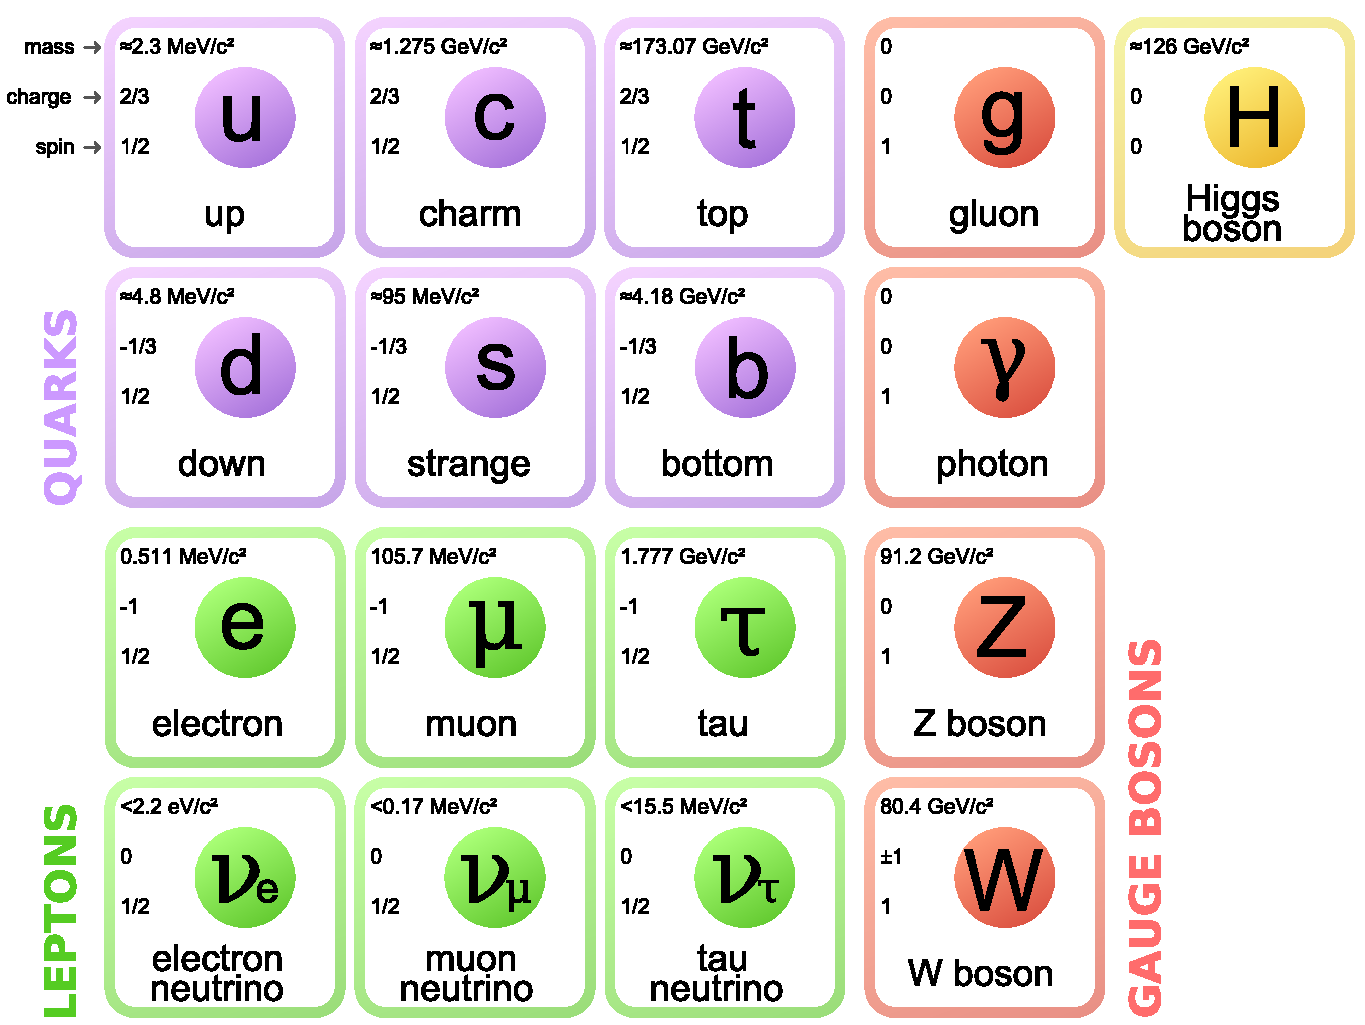
\includegraphics[width=\textwidth]{figures/standard_model.pdf}
    \caption{The particles of the standard model with information about their
        type, their mass, charge, and spin. The quarks and leptons make up
        matter, while the gauge bosons mediate interactions. The Higgs gives
        mass to the Z and W bosons.
        % https://en.wikipedia.org/wiki/Standard_Model#mediaviewer/File:Standard_Model_of_Elementary_Particles.svg
        % \TODO{Source}
    }

    \label{fig:standard_model}
\end{figure}

Our current understanding of how matter interacts at high energy is entirely
described by the standard model (SM) as constructed by Weinberg, Glashow, and
Salam \cite{glashow1961}\cite{weinberg1967}\cite{salam1968}. The model combines
three of the four fundamental forces (leaving out only gravity, which is so
weak as to be negligible) and explains almost everything we see in the
universe.

\subsection{The Electromagnetic Force}
\label{subsection:electronmagnetic_force}

The modern theory of electromagnetism began with Maxwell's theory developed in
the middle of the 19th century \cite{maxwell1863}. Maxwell was the first to
conclude that light was an electromagnetic wave, the full importance of which
was only later understood when it was discovered that the photon was the force
carrier of the electromagnetic force \cite{maxwell1865}.

In the early 20th century, Lorentz and Einstein developed relativistic
mechanics and showed that Maxwell's theory was Lorentz invariant
\cite{lorentz1899}\cite{einstein1904}. Dirac updated the theory in 1920 when he
was able to quantize the electromagnetic field as an ensemble of harmonic
oscillators \cite{dirac1927}. Dirac would go on to discover that anti-particles
were a natural consequences of his equations \cite{dirac1928}\cite{dirac1930}.
These anti-particles were found by Anderson in 1932 as he observed cosmic rays
in a cloud chamber \cite{anderson1933}.

As microwave technology improved in the 1940s, more accurate measurements of
the energy level shifts in hydrogen were made, resulting in the discovery of
the Lamb shift by Lamb and Rutherford \cite{lamb1947}. This discovery pointed
to discrepancies in the theory, discrepancies which Bethe would explain after
completing a set of non-relativistic calculations using it \cite{bethe1947}.
Bethe's work inspired multiple other physicist including Dyson, Feynman,
Schwinger, and Tomonaga to work along similar lines. They created quantum
electrodynamics, a fully relativistic and self-consistent theory of
electromagnetic interactions
\cite{tomonaga1946}\cite{schwinger1948}\cite{feynman1949}\cite{dyson1949}.

\subsection{The Weak Force}
\label{subsection:weak_force}

The need for a weak force, and hence a theory describing it, was first hinted
at by beta decay experiments in the early 1900s. These experiments culminated,
in 1914, in Chadwick's discovery that the energy spectrum of electrons ejected
in beta decay was continuous instead of a delta function as would be expected
for a two-body decay \cite{chadwick1914}. While some proposed that this
discovery indicated that momentum and energy were not conserved, Pauli proposed
an alternative: there was a neutral and invisible particle that carried away
some of the energy---the neutrino \cite{pauli1930}. Fermi began working on this
idea and invented a four fermion contact interaction in which a neutron decayed
into a proton, an electron, and a neutrino \cite{fermi1934}.

In 1947, Rochester and Butler discovered a particle that decayed to two pions
which they called the $\theta$; in 1949, Brown and Powell discovered a particle
that decayed to three pions which they called the $\tau$
\cite{Rochester1947}\cite{brown1949}. It was soon discovered that these
particles had the same mass and lifetime---indicating that they were the same
particle---but, based on their decay products, they must have different parity.
Lee and Yang proposed that perhaps there was only one particle undergoing a  a
parity violating decay \cite{lee1956}. Their idea was confirmed by Wu in 1956, who
showed that electrons were preferential emitted from \cobaltsixty in one
direction, and by Garwin, Lederman, and Weinrich in 1957, who studied \pitomunu
in a storage ring \cite{wu1956}\cite{garwin1957}.

In 1954, Yang and Mills replaced Fermi's contact interaction with a non-Abelian
gauge theory that contained a spin-1 boson to mediate the force
\cite{yang1954}. However, this boson was massless, and so the weak force's
range would have been invite. In 1960, Glashow was able to modify Yang and
Mill's theory by adding Sudarshan and Marshak's vector minus axial ($V-A$)
model to produce a unified electroweak force described by the \SUtwoUone gauge
group \cite{glashow1961}\cite{sudarshan1958}. \SUtwo is a left-handed
interaction and so violates parity as expected. Weinberg and Salamn finished up
the model in 1967 when they added the Brout, Englert, and Higgs mechanism which
made the vector bosons mass and so explained the short ranged nature of the
weak interaction
\cite{weinberg1967}\cite{salam1968}\cite{englert1964}\cite{higgs1964}.

\subsection{The Strong Force}
\label{subsection:Strong_force}

The theory of the strong force grew out of studies of atomic nuclei. In 1911,
Rutherford discovered that that atomic nucleus was a compact, positively
charged object \cite{rutherford1911}. 1917, Rutherford showed that larger
nuclei were composed of hydrogen nuclei and so discovered the proton
\cite{rutherford1919}. The discovery of the uncharged neutron in 1932 by
Chadwick indicated that the atomic nucleus was made up of multiple types of
nucleons, and that it could not be held together by the electromagnetic force
\cite{chadwick1932}. In 1934, Yukawa---having noted that Fermi's contact
interaction was too weak to hold nuclei together---tried to explain this
nuclear force using meson exchange \cite{yukawa1935}. In 1947, Lettes,
Occhialini, and Powell discovered the pion which seemed to confirm Yukawa's
theory \cite{lattes1947}.

In the 1950s and early 1960s, dozens of new mesons were discovered, indicating
the need for a new theory. Some of these new mesons seemed to have a new type
of quantum number that limited their available decays, leading them to be
called ``strange'' particles. An effort to explain these particles lead to the
Gell-Mann--Nishijima formula
\cite{nakano1953}\cite{nishijima1955}\cite{gellmann1956}. This theory lead
Gell-Mann and Ne'eman to come up with a classification scheme for mesons and
baryons based on the \SUthree which Gell-Mann named the Eightfold Way. In 1964,
Gell-Mann and Zweig realized that the Eightfold Way implied that mesons were
composed of sub-atomic particles which became known as quarks
\cite{gellmann1964}\cite{zweig1964}. This model was used to predict the
existence of the charm quark, and upon its success was incorporated with
electroweak theory to form the full \SUthreeSUtwoUone symmetry group of the
standard model.

\subsection{Experimental Verification}

The standard model has has made numerous predictions which have been borne out
by experiment. The neutral current interaction was observed by the Gargemelle
experiment at CERN in 1973 shortly after it was predicted by Weinberg, Glashow,
and Salam \cite{hasert1973}. This confirmation of their theory won the trio the
Nobel Prize in 1979. The remaining quarks were found over the next twenty
years. The charm was found at SLC and BNL in 1974 via \jpsi decays
\cite{aubert1974}\cite{augustin1974}. The bottom was discovered at FNAL in 1977
by the E288 experiment \cite{herb1977}. The final quark, the incredibly heavy
top, had to wait until 1995 to be discovered by the CDF and D0 experiments
running at the Tevatron at FNAL \cite{cdf1995}\cite{d01995}. The W and Z bosons
were discovered at CERN in 1983 at the UA1 and UA2 experiments running Super
Proton Synchrotron \cite{ua1_w}\cite{ua2_w}\cite{ua1_z}\cite{ua2_z}. These
bosons were an excellent test of the standard model as their masses could be
very exactly calculated. The discovered bosons matched the calculated masses to
high precision. The final piece of the standard model, the Higgs bosons, was
discovered by ATLAS and CMS in 2012 using the LHC at CERN
\cite{atlas_higgs}\cite{cms_higgs}. Although precession measurements of the
Higgs are still ongoing, it so far precisely matches the predictions of the
standard model.

\subsection{Components of the Standard Model}

There are two types of particles in the standard model: fermions---with half
integer spin---and bosons---with integer spin. The fermions, which make up all
of the matter in the universe, are further subdivided into two groups: leptons
and quarks.

Leptons have \spinhalf and have charge $q=-1 \text{ or } 1$ for the massive
leptons, or 0 for the neutrinos. They interact electromagnetically (if they
have a non-zero charge) and weakly. There are three generations of leptons and
each generation consists of a charged, massive lepton, and an uncharged, nearly
massless neutrino. The lightest of the charged lepton generations is the
electron, which is stable. The next two generations contain the muon and the
tau, which are unstable and eventually decay to electrons. The tau, being very
heavy, decays quickly, while the muon is stable long enough to escape a
particle detector. Massive leptons are important in particle detection as they
provide a very clean decay signature. Neutrinos are very difficult to detect in
particle detectors, and so their presence is inferred from the missing energy
in the vector sum of all particles in the collision. This analysis uses
electrons to make its measurement.

Quarks also have \spinhalf although, unlike the leptons, their charge is
fractional and so takes values of $q = 2/3 \text{ or } -1/3$. They interact
strongly, electromagnetically, and weakly. There are three generations of
quarks, with each successive generation having a higher mass constituents. The
first generation consists of the up and down (u and d) quarks. These quarks are
stable and make up protons and neutrons, as well as pions. The next generation
of quarks contains the charm and the strange (c and s). They form heavier
states that decay quickly like the \jpsi and kaons. The final generation
consist of the heavy bottom (b), and the exteriorly heavy top (t)---the most
massive particle in the standard model. Bottom quarks can form bound states,
but top quarks are so heavy they decay before any bound states can form.

Quarks carry color charge, of which there are three: red (r),
blue (b), and green (g). Strongly interacting objects obey confinement, which
means that only color neutral (colorless) states are allowed. Because of
confinement, quarks bind together into colorless composite particles. These
particles are called mesons---with two quarks (\qqbar)---and baryons---with
three quarks (\baryon). When an object containing quarks breaks up, the
individual colored fragments will create additional colored objects to maintain
their colorless state. This leads to the formation of ``jets'' which are sprays
of high energy particles that originate from one of these fragments as it tries
to maintain its colorless state.

Bosons are the second type of particle in the standard model. They are further
subdivided into gauge bosons---which mediate the three forces---and the Higgs
boson---which gives mass to the W and Z bosons.

The gauge boson that mediates the strong force is the gluon. Gluons interact
with objects that carry color, and are themselves carriers of color, allowing
gluons to interact not only with quarks but with other gluons. Gluons can have
any one of eight different possible color-anticolor superpositions that form a
color-octet. This number comes from the number of generators of \SUthree. Such
octets are not unique, but a commonly used definition is listed in
\TAB~\ref{table:gluon_color}.

\begin{table}[h]
\centering
\begin{center}
    \begin{tabular}{ c  c }
        $\left( \xxbar{r}{b} + \xxbar{b}{r} \right) / \sqrt{2}$ &
        $-i \left( \xxbar{r}{b} - \xxbar{b}{r} \right) / \sqrt{2}$ \\
        $\left( \xxbar{r}{g} + \xxbar{g}{r} \right) / \sqrt{2}$ &
        $-i \left( \xxbar{r}{g} - \xxbar{g}{r} \right) / \sqrt{2}$ \\
        $\left( \xxbar{b}{g} + \xxbar{g}{b} \right) / \sqrt{2}$ &
        $-i \left( \xxbar{b}{g} - \xxbar{g}{b} \right) / \sqrt{2}$ \\
        $\left( \xxbar{r}{r} - \xxbar{b}{b} \right) / \sqrt{2}$ &
        $\left( \xxbar{r}{r} - 2\xxbar{b}{b} + \xxbar{g}{g} \right) / \sqrt{6}$ \\
    \end{tabular}
    \caption{
        One of the possible color-octets. The colors are red ($r$), blue ($b$),
        green ($g$), and their anti-colors ($\overline{r}$, $\overline{b}$, and
        $\overline{g}$) .
    }
\label{table:gluon_color}
\end{center}
\end{table}

There are four gauge bosons that mediate the electroweak interaction: the photon
(\photon), the \Z, and the \Wpm. The photon and the \Z are uncharged, while the
\Wpm carries charge. The \W and \Z are not the particles described by the
\SUtwoUone group, but are instead linear combinations of these fields created
through combination with the Higgs mechanism. The \W participates in
interactions that change quark and lepton flavor, for example \ttoWb or
\mutoWnu.

The \Z boson acts as an excellent probe of precision physics as its well
measured mass (\Zmass) and its sharp width (\Zwidth) make it easy to identify
from its decay products \cite{pdg2014}. In a hadron collider the most common
\Ztoqq decay mode is difficult to select, and so \Ztoll decay modes are
preferred. In this analysis we look at the \Ztoee decay mode. A few common
decay modes and their branching fraction are listed in
\TAB~\ref{table:z_decays}.

\begin{table}[h]
\centering
\begin{center}
    \begin{tabular}{ l  r }
        Mode & Fraction $\left( \Gamma_{i} / \Gamma \right)$ \\ \hline
        $\Ztoqq$ & $69.91 \pm 0.06\%$ \\
        $\Ztoee$ & $3.363 \pm 0.004\%$ \\
        $\Ztomumu$ & $3.366 \pm 0.007\%$ \\
        $\Ztotautau$ & $3.370 \pm 0.008\%$ \\
        $\Ztonunu$ & $20.00 \pm 0.06\%$ \\
    \end{tabular}
    \caption{
        Selected decay modes of the \Z boson.
    }
\label{table:z_decays}
\end{center}
\end{table}


% The experiment, and how we use it
\chapter{The CMS Experiment}
\label{experiment_chapter}

\TODO{Jeremy suggests focusing the chapter more on the subdectors we use: ECAL
and Tracker}

\section{The Large Hadron Collider}
\label{lhc_section}

\begin{figure}[tb]
    \centering
    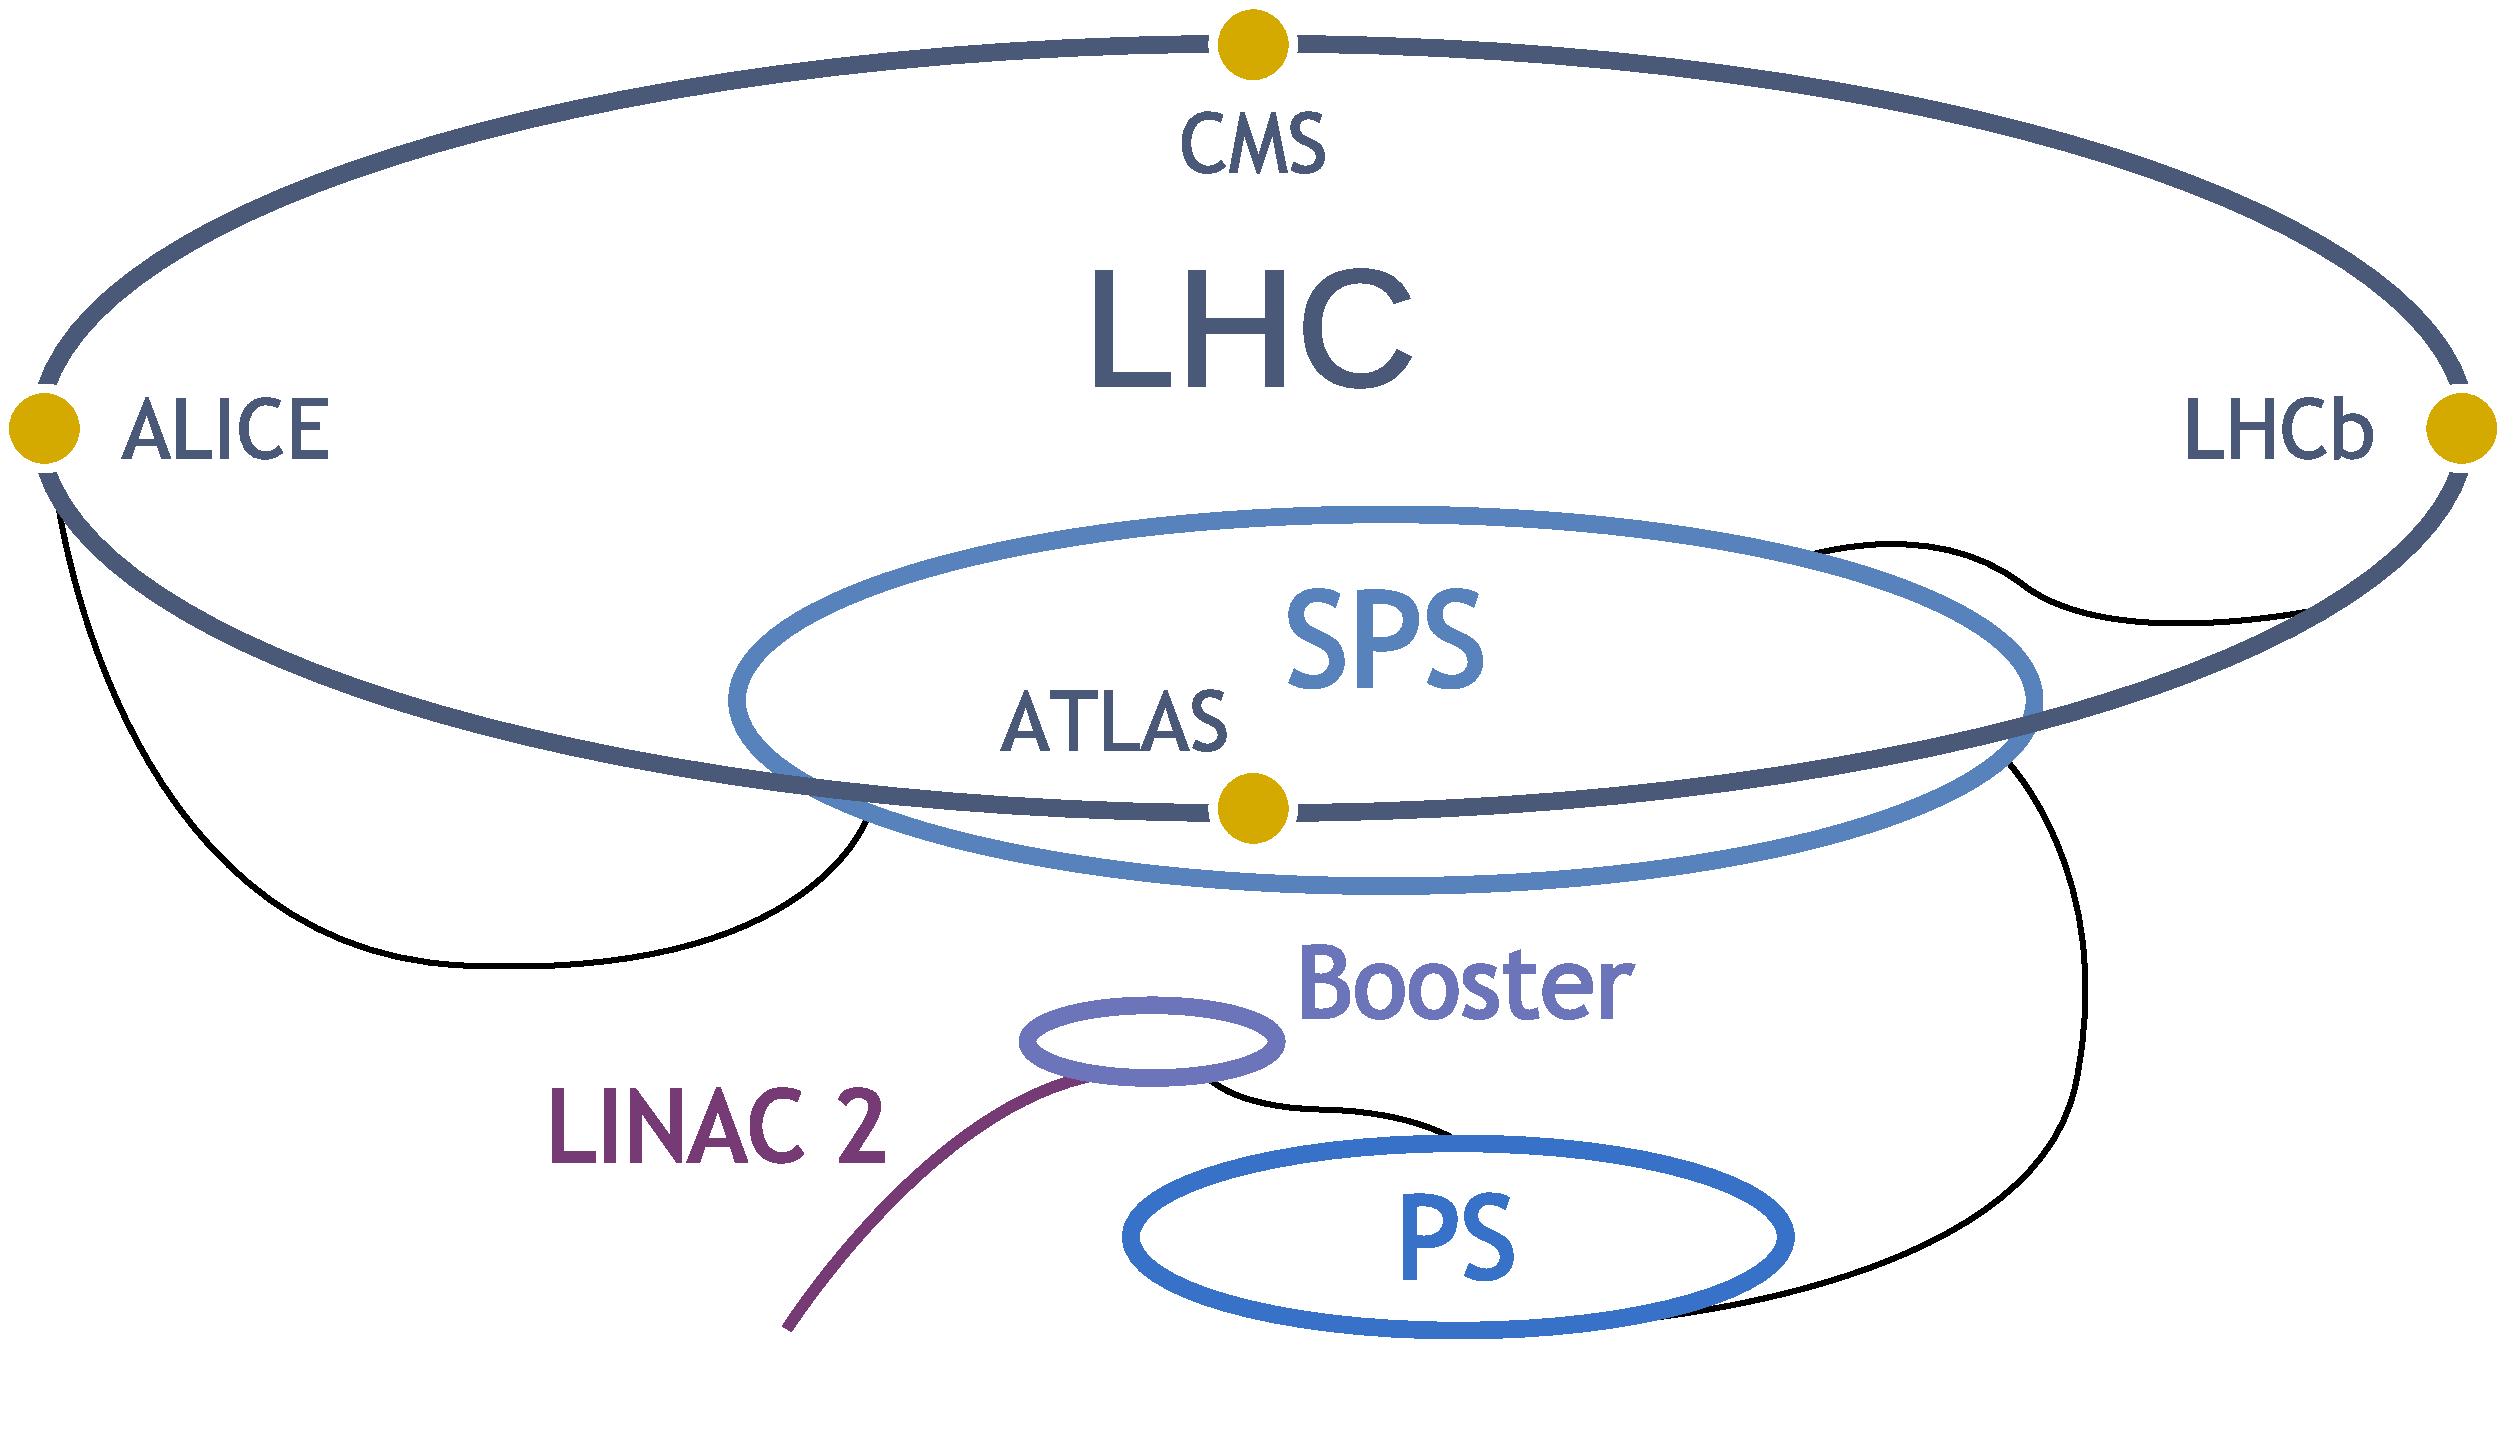
\includegraphics[width=\textwidth]{figures/alex_lhc_layout.pdf}
    \caption{The LHC and its accelerator chain.}
    \label{fig:lhc_layout}
\end{figure}

The Large Hadron Collider (LHC) is the world's highest energy and largest
particle accelerator with a maximum design center-of-mass energy of 14\TeV and
a radius of 2804\meters \cite{bruning2004}. It collides protons on protons, as
well as protons on ionized lead (\lead) and \lead on \lead. In 2012, when LHC
most recently produced collisions, it had a center of mass energy of 8\TeV;
when it turns back on in 2015 after upgrades, it will run at 13\TeV. The LHC is
located near Geneva, Switzerland, although it is so large that most of the
accelerator (including \pointfive, where the CMS detector is located) is in
France.

A number of smaller accelerators are used together in series to accelerate
protons to the energies necessary to be injected into the LHC. The first step
is a linear accelerator, \linactwo, which accelerates protons from rest to
50\MeV. These protons are then injected into a chain of three circular
accelerators, each injecting into the next. The first of these accelerators is
the Proton Synchrotron Booster (PSB) which accelerates the protons to 1.4\GeV.
The second is the Proton Synchrotron (PS) which accelerates the protons to
26\GeV. The third and final accelerator is the Super Proton Synchrotron (SPS)
which accelerates the protons to 450\GeV and injects directly into the LHC.

Bunches of protons are accelerated using this system and injected into the LHC
to form two counter-rotating beams. When the desired number of bunches have
been injected into the LHC, the LHC accelerates them to 4\TeV. When the beams
have reached their nominal energy, they are focused and brought into collision
at four different points on the ring where the various experiments (\ALICE,
\ATLAS, \LHCB, and CMS) are located. A cartoon layout of the LHC and its
accelerator chain is shown in \FIG~\ref{fig:lhc_layout}.

The beams are steered around the accelerator ring by a series of
superconducting, dipole magnets. When running at a center-of-mass energy of
8\TeV, these magnets operate at roughly 7.5\Tesla. There are also quadrapoles
and some higher order magnets around the ring used to focus the beams \TODO{and
correct for lattice defects}. The bunches of protons are accelerated by 16
superconducting radio frequency cavities. These cavities accelerate slower
protons while slowing faster ones, thereby keeping the proton bunches compact
in both real and momentum space. There is room for 2808 bunches in LHC
separated by 25\ns, although in 2012 50\ns spacing was used and so there were
only 1374 bunches of which 1368 were brought into collision at CMS and \ATLAS.

The LHC is also the highest luminosity collider in the world. The instantaneous
luminosity is given by
\begin{equation}
    \luminosity = f n \frac{N^{2}}{\sigma}
\end{equation}
where $f$ is the frequency of interaction (which is fixed by the LHC's
circumference), $n$ is the number of bunches in a beam, $N$ is the number of
protons per bunch (with the $N^{2}$ coming from the assumption that there are
the same number of protons in the two colliding bunches), and $\sigma$ is the
area profile of the beams. 

Although a higher luminosity means more particles are produced and more data
can be collected, the maximum luminosity is limited by several practical
factors. The first factor is cost; a higher luminosity general requires a more
expensive machine as the ring is either made larger or the technology needed to
run the machine is made more complex. The cost of the detectors also increases
as they require more channels to separate the larger number of particles,
faster readout to deal with the increased event rate, and higher bandwidth to
read out the larger numbers of channels. The second is the challenge that
higher luminosities present to the analyzers. The luminosity can be increased
by increasing the number of protons in a bunch or by squeezing the bunches more
tightly, but eventually the probability of getting multiple proton-proton
interactions per bunch crossing becomes large, leading to a phenomenon known as
pileup. These extra interactions add additional particles to the detector and
can make it difficult to separate interesting events from uninteresting
background. The luminosity can also be increased by increasing the number of
bunches in the machine, but this decreases the time between the collisions and
leads to a phenomenon known as out-of-time pileup which can also obscure
interesting events. The third factor is that high radiation doses damage the
detectors. Plastic and crystal scintillators darken while silicon detectors
become noisy. This forces the detectors to replace their components more
frequently.

In 2012, the optimal luminosity was achieved by running with bunches spaced by
50\ns instead of the design nominal bunch spacing of 25\ns. This larger bunch
spacing was chosen because at smaller spacing the bunches were destabilized by
electron clouds---clouds of electrons knocked out of the beam pipe by the
beam's synchrotron radiation, as well as secondary electrons freed when the
photoelectrons impact their surroundings.

\section{The Compact Muon Solenoid}
\label{cms_section}

\begin{figure}[tb]
    \centering
    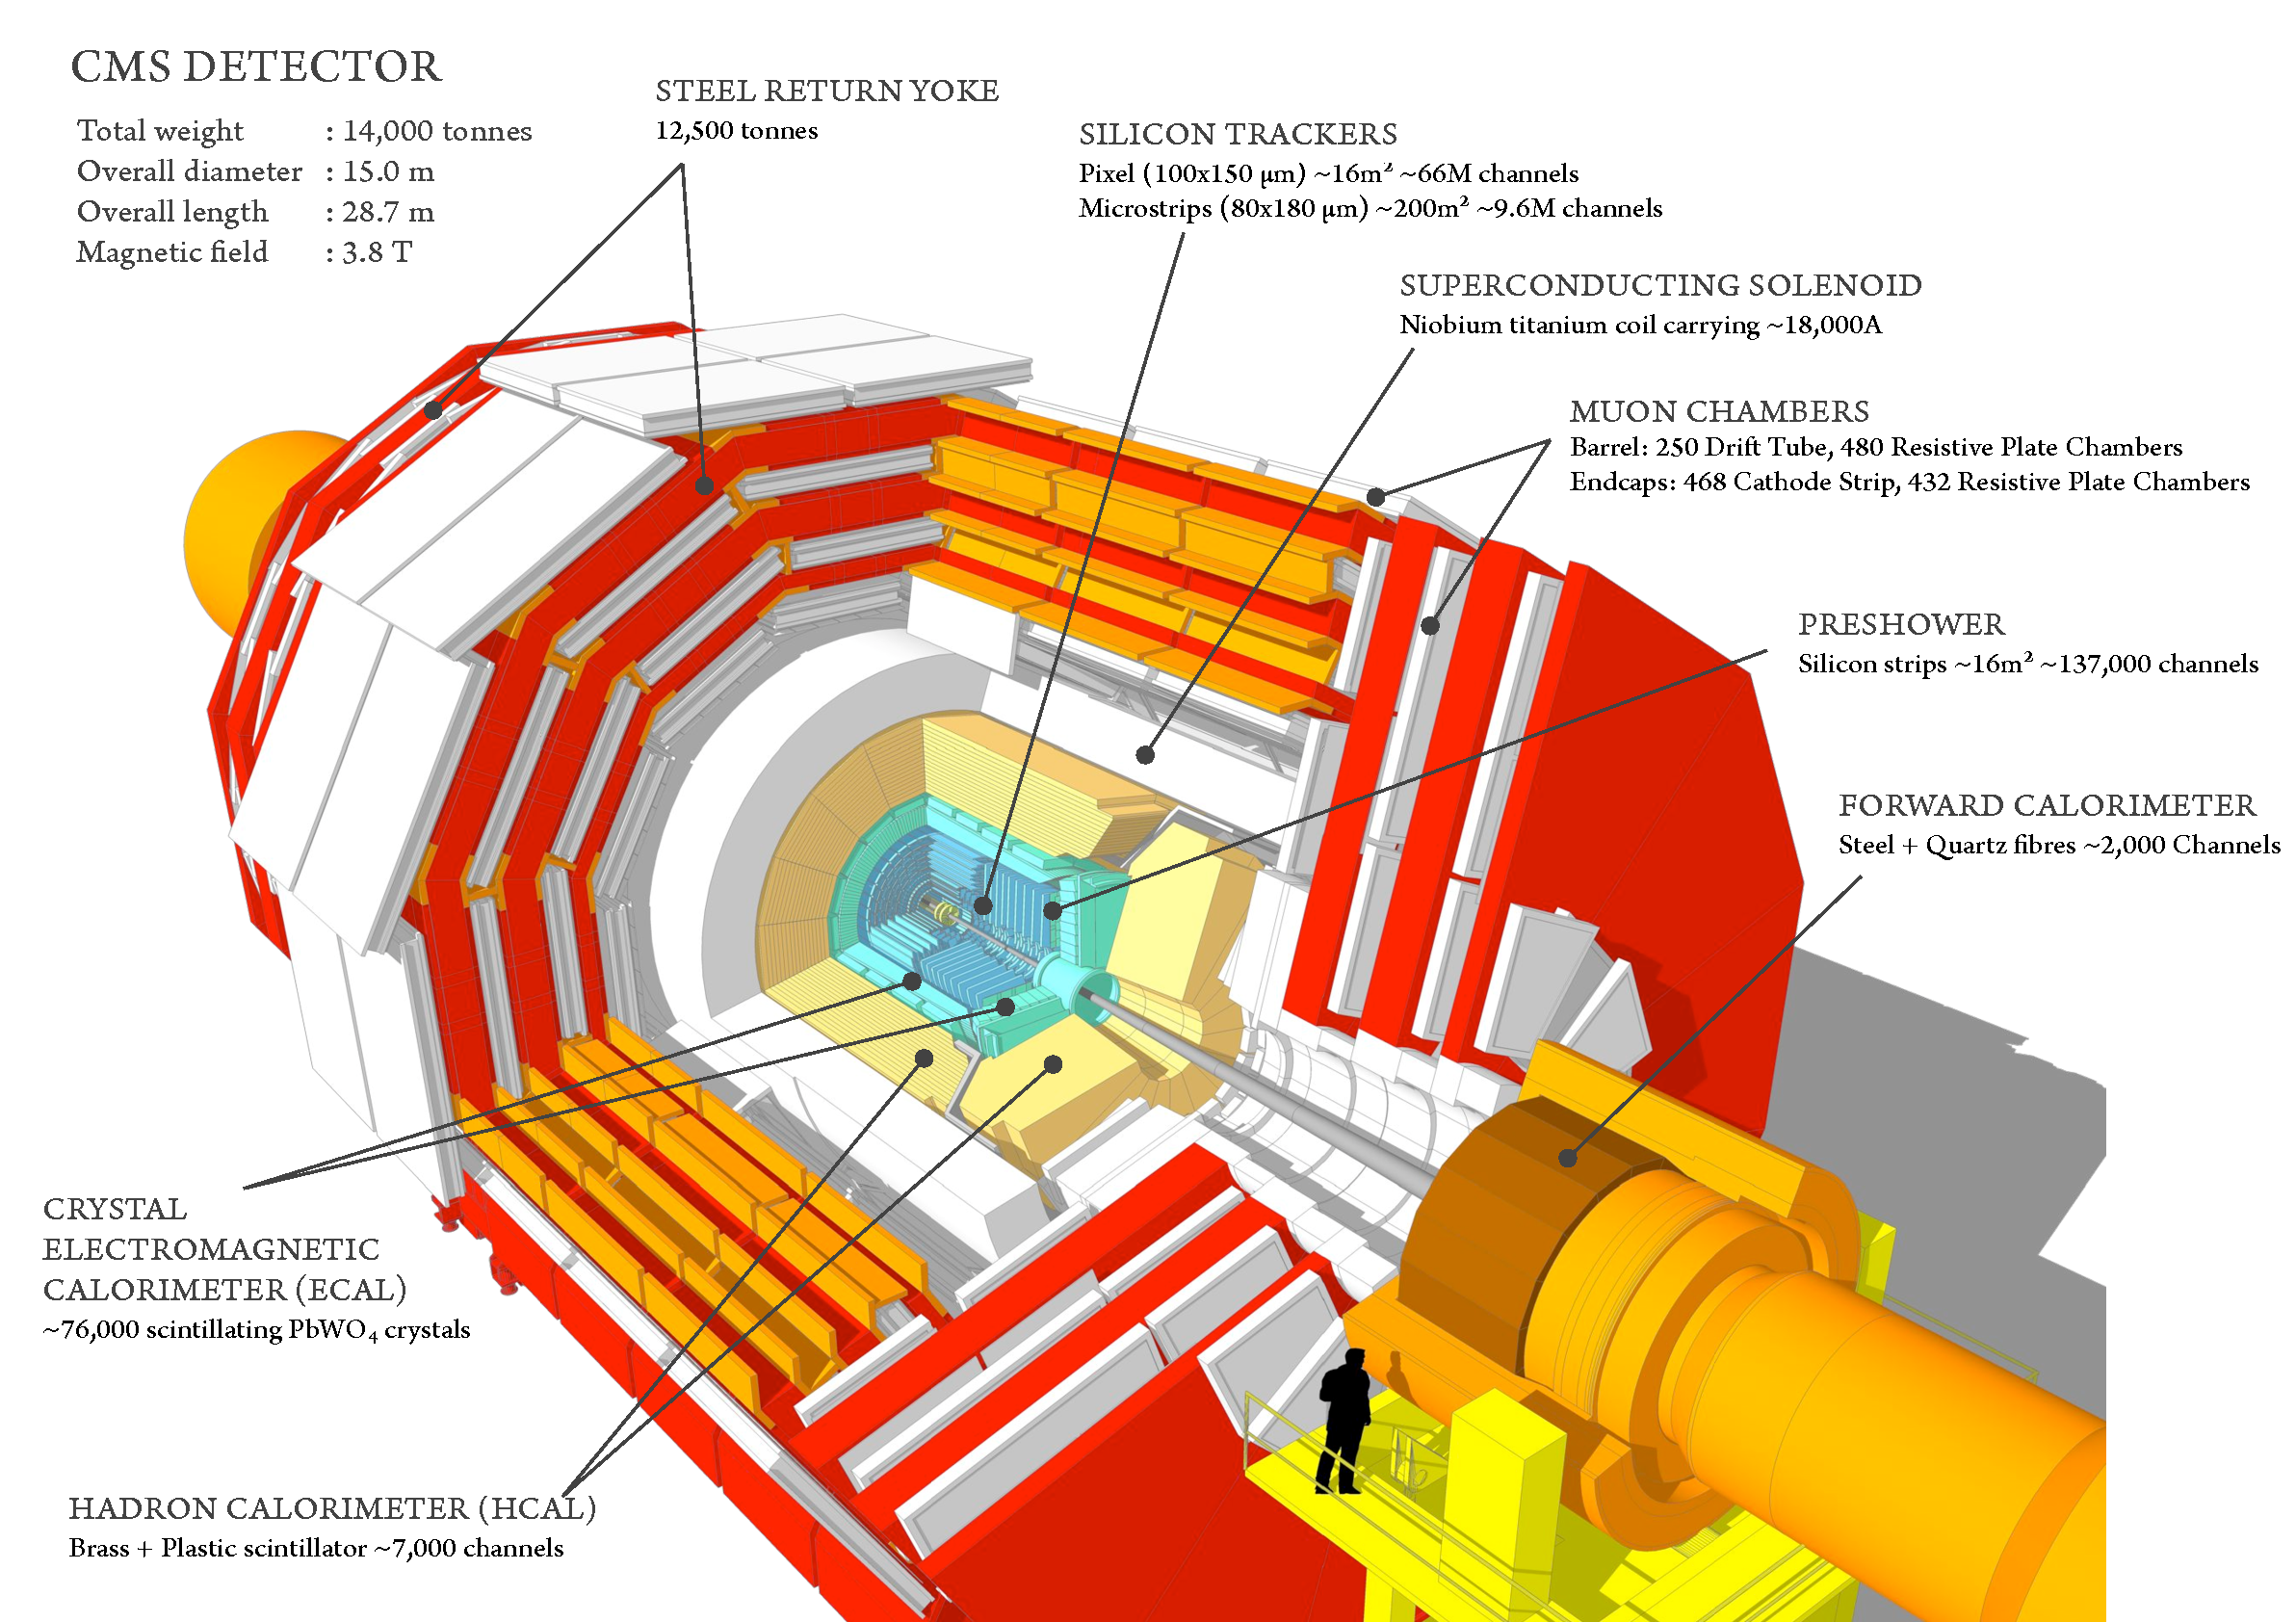
\includegraphics[width=\textwidth]{figures/cms_cutaway.png}
    \caption{A cut-away view of the CMS.}
    \label{fig:cms_cutaway}
\end{figure}

The Compact Muon Solenoid (CMS) is one of two general-purpose particle
detectors built on the LHC ring \cite{cms_tdr_1}\cite{cms_tdr_2}. CMS is
designed to detect the very high energy, sub-atomic particles that are produced
in the LHC's proton-proton collisions. CMS is designed to have a high
acceptance and efficiency for these collisions. Here acceptance indicates the
area in both physical space as well as the area in energy and momentum space in
which the detector can detect particles. Efficiency is the probability that a
particle in CMS's acceptance region is properly measured. In order to have a
high acceptance and efficiency, CMS must be both large---to cover a large area
of physical space---and dense---to cover a large area in momentum and energy
space. CMS is 21.6\meters in length, 14.6\meters in diameter, and weighs
14\kilotonne.

CMS is built as a series of nested, finite cylinders, where each cylinder is a
separate subdetector. The beams enter the detector along the axis of the
cylinder. The collision point is in the center. There are a pair of endcaps on
either side of the cylinder to increase the acceptance of the detector. The
endcaps and central region of the cylinder (call the barrel) overlap to prevent
particles from escaping undetected through the crack. A cutaway of the detector
is shown in \FIG~\ref{fig:cms_cutaway}.

The coordinate system used by CMS is as follows: the origin is the nominal
interaction point at the center of CMS, the \xaxis is defined to point to the
center of the LHC ring, the \yaxis is defined as vertically up, and the \zaxis
points counter-clockwise and tangent to the LHC ring such that it forms a
right-handed coordinate system with the \xaxis and \yaxis. CMS uses a
cylindrical coordinate system with coordinates ($\eta$, $\phi$). The azimuthal
angel $\phi$ is in the \xyplane measured from the \xaxis so that $\phi=\pi/2$
at that \xaxis, while $\eta$ is the pseudorapidity defined by

\begin{equation}
    \eta = -\logn \tan \frac{\theta}{2}
\end{equation}

where $\theta$ is the polar angle with respects to the \zaxis. The magnetic
field points along the \zaxis.

\subsection{Inner Tracking System}

\TODO{$\eta$ coverage, electric field, performance}

The inner tracking system, referred to as the tracker, is the subdetector
closest to the interaction point. The tracker's primary purpose is to measure
the charge of particles, the momentum of these same particles, and the location
of interaction vertices---both the primary vertex, the various additional
proton-proton vertices from pileup, and the vertices of long-lived particles
like b mesons. The tracker consists two types of silicon detectors: silicon
pixels and silicon strips.

\subsubsection{Pixel Tracker}

\begin{figure}[tb]
    \centering
    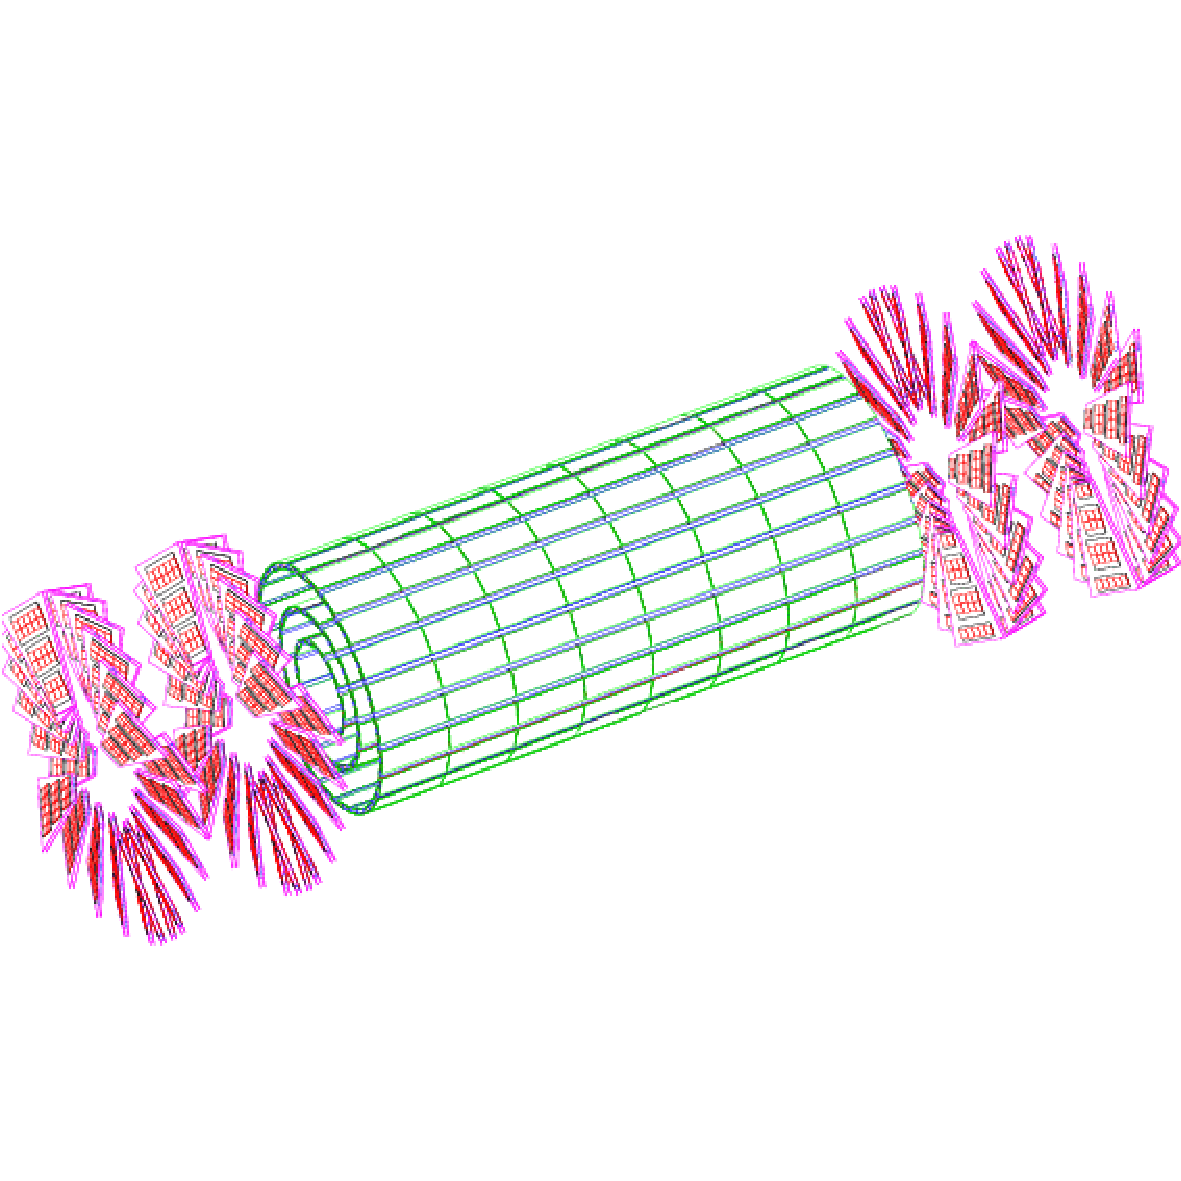
\includegraphics[width=\textwidth]{figures/pixel_layout.pdf}
    \caption{A cross-sectional view of the CMS pixel Tracker.}
    \label{fig:pixel_layout}
\end{figure}

The silicon pixels are used in the region closest to the beam pipe where the
particle flux is the highest and hence the finest granularity is needed. Their
primary purpose is to very accurately locate the primary and secondary vertices
in a collision.

There are three barrel layers of the pixel tracker at radii of of 4.3, 7.3, and
10.2\centimeters, each with a length of 53\centimeters. At each end, there are
two endcap annular disks as well placed at $|\coordz|=$ 34.5 and
46.5\centimeters. Each of these disks has an inner radius of 6\centimeters and
an outer radius of 15\centimeters.

Each pixel has an area of $100 \times 150 \micrometers^{2}$, but the resolution
of the tracker is better than that because of charge sharing. If a charged
particle ionizes multiple pixels, then a weighted average of the charges can be
used to get sub-pixel resolution on the location of the hit. In order to
increase the charge sharing, a large Lorentz angle (23\degrees) is used. The
blades which make up the endcap disks are fanned out in a turbine-like geometry
with a rotation of 20\degrees to benefit from the same effect. The layout of
the pixel detector is shown in \FIG~\ref{fig:pixel_layout}.

\subsubsection{Strip Tracker}

\begin{figure}[tb]
    \centering
    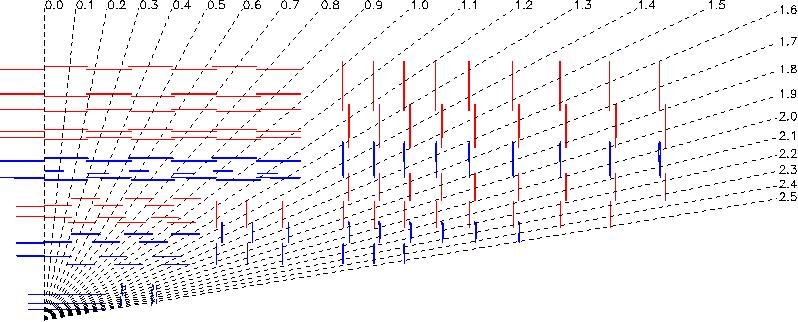
\includegraphics[width=\textwidth]{figures/strip_layout.jpg}
    \caption{A quarter cross-section view of the CMS strip tracker.}
    \label{fig:strip_layout}
\end{figure}

The silicon strips are used further from the beam pipe than the pixels and
cover a much large radius from the beam pipe. The strip tracker has 200 times
the area of the pixel tracker, and so it was not economically feasible to use
the more expensive pixel detectors in this region. The strips' primary purpose
is to measure the momentum and curvature of the charged particles by extending
the tracker's coverage over a larger radius.

Although the strips provide only two points in space to locate a hit (as
compared to three for the pixels), this coarser geometry is adequate because of
the much lower particle flux in this region of the detector. For the momentum,
the location of the hit in the \rphiplane is the most important information,
and so the strips are aligned parallel to the magnetic field. \TODO{Explain
more?}

The strip tracker is itself divided into multiple components. In the barrel
there is the TIB (Tracker Inner Barrel) and the TOB (Tracker Outer Barrel). The
TIB consists of four layers and has coverage up to $|\coordz|<$ 65\centimeters.
The silicon sensors making up the TIB have a strip pitch which varies between
80 to 120\micrometers and have a thickness of 320\micrometers. The first two
layers are constructed with a double layer of modules with a stereo angle of
100\millirads, providing information about the location of the hit in both the
\coordrphi and \rzplane. The TOB consists of six layers and has coverage up to
$|\coordz|<$ 110\centimeters. The TOB has a strip pitch which varies between
120 and 180\micrometers and have a thickness of 500\micrometers. The thicker
sensors are able to be used in this region because the radiation levels are
lower. Having a thicker sensors helps to maintain a high signal-to-noise ratio.
Just like the TIB, the first two layers of the TOB are also built with a double
layer of modules with a stereo angle of 100\millirads.

The ends of the strip tracker consists of the TEC (Tracker Endcap) and the TID
(Tracker Inner Disk). The TEC consists of nine disks in the region
120\centimeters $< |\coordz| <$ 280\centimeters. The TID consists of three
disks in between the end of the TIB and the start of the TEC. The TEC and TID
consist of modules arrayed in rings around the beam line, with the face of each
module pointed towards the interaction point so that they have varying
orientations depending on their distance from the interaction point. The first
two rings of the TID and the first, second, and fifth rings of the TEC are
built with double layer of modules. The modules in the TID and the first three
disks of the TEC have a thickness of 320\micrometers while the rest of the
modules in the TEC have a thickness of 500\micrometers. The strip pitch in the
TID and the first three disks of the TEC have a strip pitch which varies
between 97 and 143\micrometers while the rest of the modules in the TEC have a
strip pitch between 143 and 183\micrometers. The layout of the entire tracker,
including the strip tracker, is shown in \FIG~\ref{fig:strip_layout}.

\subsection{Electromagnetic Calorimeter}

\begin{figure}[tb]
    \centering
    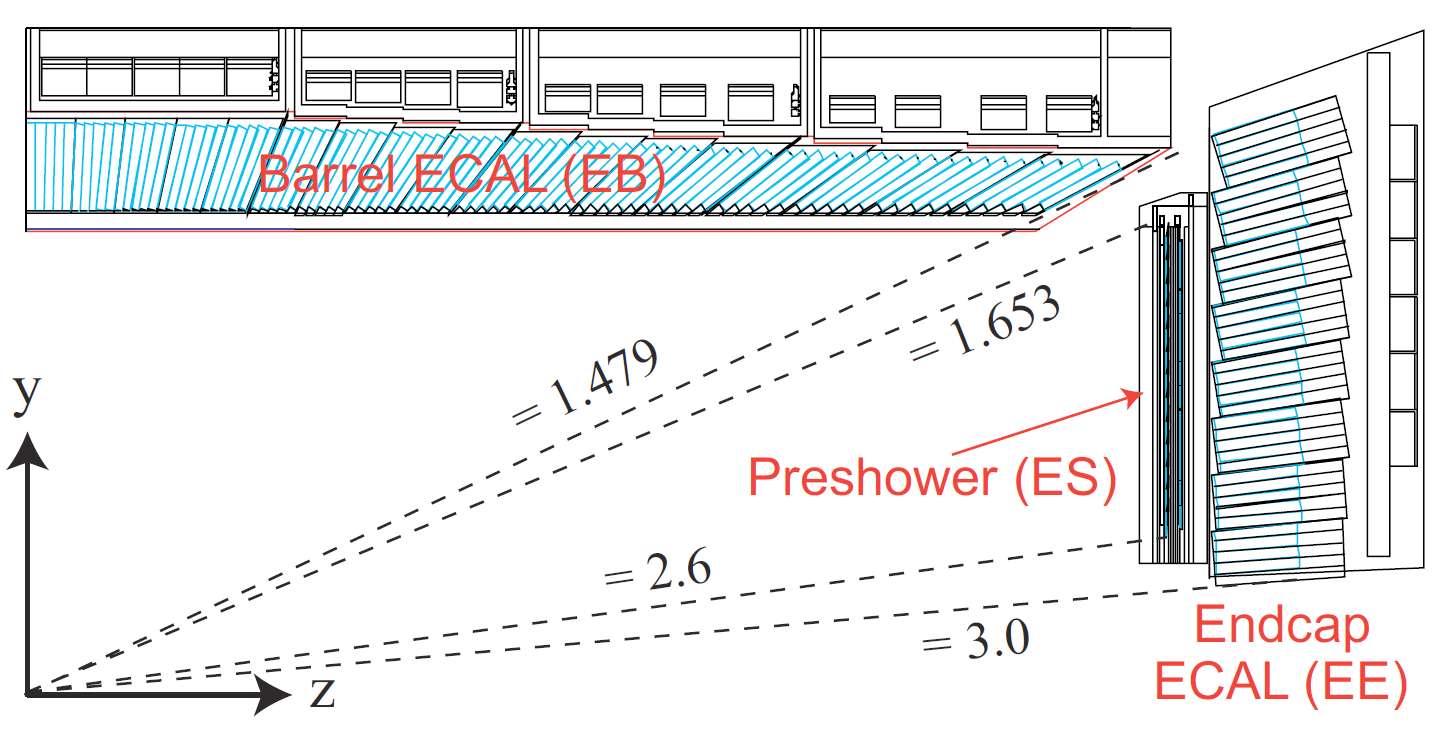
\includegraphics[width=\textwidth]{figures/ecal_layout.png}
    \caption{A cross-sectional view of the CMS Electromagnetic calorimeter.}
    \label{fig:ecal_layout}
\end{figure}

The electromagnetic calorimeter (ECAL) in CMS is built around the tracker. Its
primary purpose is to measure the energy of electrons and photons. ECAL's
design was motivated by the need to measure the \higgstogammagamma decay. In
order to have suitable energy resolution, most of the energy of the particle
must be contained within the calorimeter, and so ECAL had to be very dense. In
order to separate the highly boosted photons, ECAL needed to have fine
granularity. Due to the high luminosity of the LHC, ECAL had to be radiation
hard.

In order to meet the three design goals, ECAL is made out of 75848
scintillating lead tungstate (\leadtungstate) crystals: 61200 in the barrel,
and 7324 in each of the two endcaps. The radiation length in lead tungstate is
short ($\radlength = 0.89\centimeters$) allowing ECAL to be compact (a
necessity since it must fit within the solenoid) but still contain $\approx
25\radlength$ of scintillator. The \Moliere radius is also small
(2.2\centimeters) allowing showers to be contained within each crystal. Lead
tungstate is also radiation hard (up to 10\megarads). While lead tungstate has
a fast response (80\% of light is given off within 25\ns), it does not produce
very much light ($30 \photon / \MeV$) and so sensitive photodetectors that can
operate within a strong magnetic field are required. In the barrel avalanche
photodiodes are used, and in the endcaps vacuum phototriodes are used.

The ECAL barrel detector (EB) has an inner radius of 129\centimeters and covers
a pseudorapidity range from $0 < |\eta| < 1.479$. It is composed of 36
identical ``supermodules'' each covering half the barrel's length and 1/18th of
the barrel's circumference. The crystals used in the EB have a front face
cross-section of $22 \times 22\millimeters^{2}$ and a length of
230\millimeters. They cover 1\degrees in $\Delta \eta$ and $\Delta \phi$. The
crystals are tilted with their axis 3\degrees off from the vertex region in
order to obscure the small gaps between crystals from particles leaving the
interaction point.

The ECAL endcap detectors (EE) are located with their front face at
$|z|=314\centimeters$ and cover a pseudorapidity range of $1.479 < |\eta| <
3.0$. Each endcap is composed of two ``Dees'' consisting of semi-circular
aluminum plates with crystals mounted on them. The crystals used in the EE have
a front face cross-section of $28.6 \times 28.6\millimeters^{2}$ and a length
of 220\millimeters. Unlike in EB, where the crystals are arranged in an
\coordetaphi~grid, the crystals in EE are arranged in an \coordxy~grid. Like
the EB crystals, the EE crystals also off-point from the vertex region.

In addition to EB and EE, there is a smaller subdetector, the preshower (ES),
placed in front of EE. It is made of lead and silicon and has higher
granularity then EE. It was designed to help differentiate \pitogammagamma
decays from \higgstogammagamma decays.

The layout of ECAL is shown in \FIG~\ref{fig:ecal_layout}.

\subsection{Hadronic Calorimeter}

\begin{figure}[tb]
    \centering
    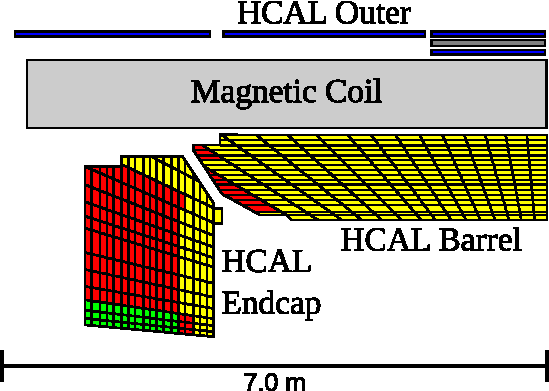
\includegraphics[width=\textwidth]{figures/hcal_cross_section.pdf}
    \caption{A cross-sectional view of the CMS hadronic calorimeter.}
    \label{fig:hcal_layout}
\end{figure}

The hadronic calorimeter (HCAL) in CMS is built around ECAL and inside the
solenoid. HCAL's primary purpose is to measure the energy of the various
strongly-interacting particles created by the collision. HCAL must have good
containment of hadronic particles so that the missing transverse energy, \MET,
of an event can be accurately measured. This variable is useful for identifying
non-interacting particles like neutrinos, dark matter, or other long-lived
exotic particles.

HCAL is a sampling calorimeter which is appealing because that allowed it to be
made compact (and HCAL must fit within the magnet), cheap (ECAL was expensive,
so savings elsewhere were necessary), and with good enough resolution, since
the resolution is dominated by the hadronic over electromagnetic (\HOverE)
correction anyway. This correction arises from the fact that the detector
response from electromagnetic interactions is different than for hadronic
interactions, and from the fact that there are statistical fluctuations in the
number of neutral pions---which decay to two photons and so interact
electromagnetically---and charged pions---which interact hadronically---which
make up a hadronic shower in HCAL on an event-by-event basis. These differences
are corrected for in aggregate, with the effect of broadening the calorimeter's
resolution.

\subsubsection{Hadron Barrel, Hadron Endcaps, and Hadron Outer}

The hadron barrel (HB) and hadron endcaps (HE) detectors are constructed of
alternating layers of absorber and scintillators. The absorber is made of brass
because it has a short interaction length, is easy to machine, and is
nonmagnetic. In between, the showers are sampled by plastic scintillator tiles
read out with embedded wavelength-shifting fibers. The wavelength-shifting
fibers are spliced to clear fibers outside the scintillator which carry the
signal to the readout system. The light is readout by multi-channel hybrid
photodiodes. The hadron outer (HO) detector is a layer of plastic scintillator
on the outside of the solenoid before the muon systems begin. It serves as a
``tail catcher'' by measuring the hadronic energy leaking through HCAL and
interacting with the magnet.

%HB consists of 72 segments of 32 towers with each segment covering a
%pseudorapidity range from $0 < |\eta| < 1.4$. The size of each tower is $\Delta
%\eta \times \Delta \phi = 0.087 \times 0.087$. In HB there are 15 brass plates,
%each with a thickness of 5\centimeters and two stainless steel plates, one on
%the inner face and one on the outer face to add mechanical strength. The first
%scintillator plate has a thickness of 9\millimeters, all others have a
%thickness of 3.7\millimeters. HE, unlike EE, is constructed to form a grid in
%\coordetaphi. It covers a rapidity region from $1.3 < |\eta| < 3$. For the
%lowest values of $\eta$ its channel size roughly matches the barrel, but this
%size grows at higher $\eta$.

\subsubsection{Hadron Forward}

The hadron forward (HF) calorimeter is the most forward of of the detectors
that make up HCAL, and the one of the most forward detectors in CMS. HF is
located 11.2\meters from the interaction point. It covers a pseudorapidity
range of $3 < |\eta| < 5$ and so receives a very high particle flux. HF must be
very radiation hard in order to survive in this environment. HF is constructed
of steel and quartz. The signal in HF originates from \Cherenkov light in the
quartz.

The steel absorb is 1.65\meters thick. Placed within the absorber are quartz
fibers which are 0.6\millimeters in diameter and oriented parallel to the
\zaxis. These fibers are arranged in a square grid 5\millimeters apart. There
are two lengths of fibers: ``long'' 1.65\meters ones and ``short'' 1.43\meters
ones. These different lengths allow HF to sample showers at two different
depths.

The layout of HCAL is shown in \FIG~\ref{fig:hcal_layout}.

\subsection{Magnet}

The central feature of CMS, both from a design standpoint and structurally, is
the large superconducting solenoid magnet. A high strength magnetic field is
required in CMS in order to achieve a momentum resolution of $\Delta \momentum
/ \momentum \approx 10\%$ for muons with $\momentum = 1 \TeVc$. The momentum of
these muons must be measured using their curvature in the tracker and the muon
chambers. Additionally, the magnetic field allows the charge of particles to be
measured by the direction in which their tracks curve. The solenoid provides a
magnetic field for all of the components inside the bore of the magnet. The
fringing fields are collected and returned by the iron return yokes which also
support the muon chambers. In this way a field is provided for the muon
chambers without requiring an additional magnet.

The solenoid is 12.9\meters long with an inner bore of 5.9\meters. It generates
a 3.8\tesla field using 2168 turns of conductor which carry 19.5\kiloamps. The
total stored energy is 2.7\gigajoules. The solenoid is encased in aluminum to
help dissipate heat and add strength. This entire assembly is enclosed in a
stainless steel cryostat. The cryostat must be exceptionally strong because it
not only supports the solenoid, but also all of the barrel subdetectors (HCAL,
ECAL, and the tracker) that are mounted within it. The calorimeters and the
tracker are mounted within the solenoid in order minimize the un-instrumented
mass---where particles could lose energy due to interactions---between the
calorimeters and the collision region.

\subsection{Muon System}

\begin{figure}[tb]
    \centering
    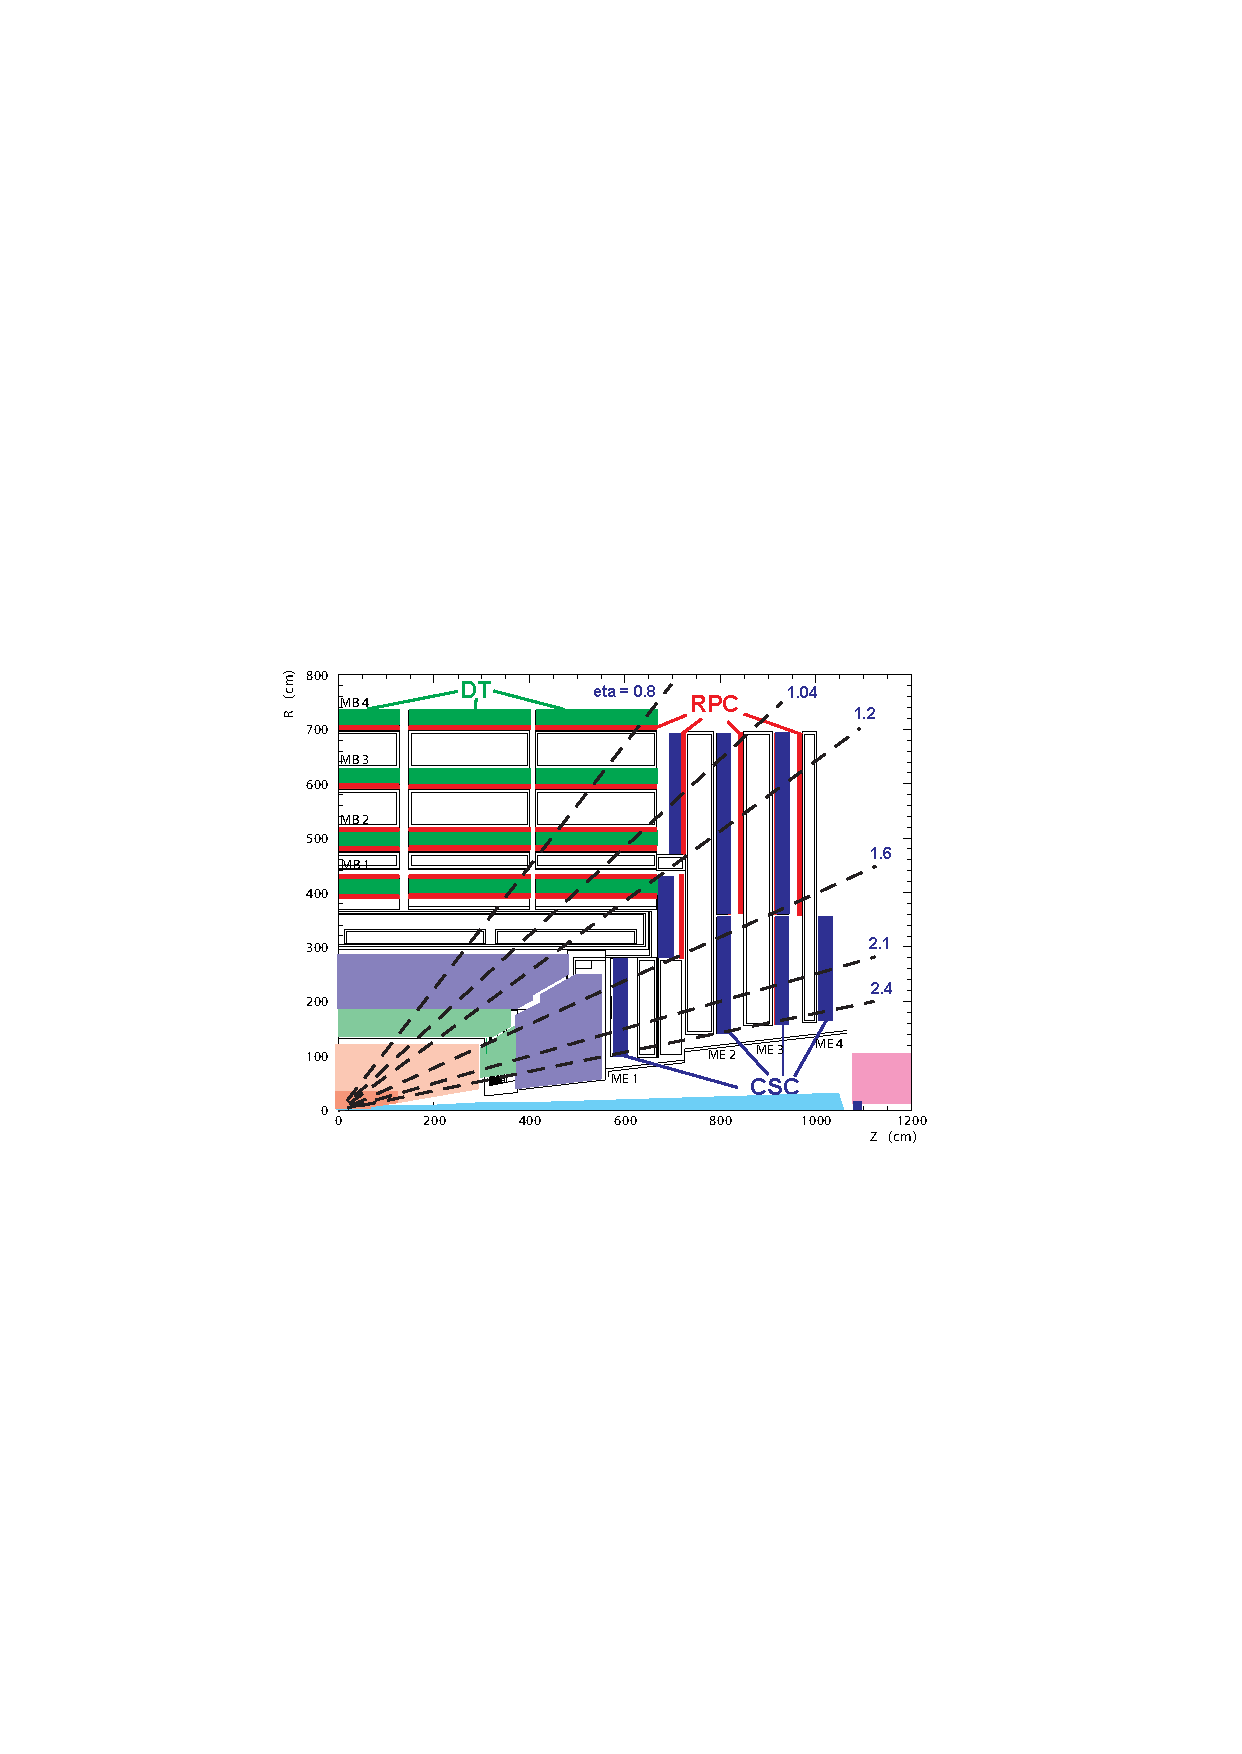
\includegraphics[width=\textwidth]{figures/muon_layout.pdf}
    \caption{A cross-sectional view of the CMS muon system.}
    \label{fig:muon_layout}
\end{figure}

The muon system is the outer most subdetector of CMS. Its primary purpose is to
assist in measuring high momentum muons and allow triggering on muons. Without
the muon system, no triggering on muons would be possible because they are
minimum ionizing particles in the calorimeters and the tracker can not be read
out quickly enough to use in triggering. For high energy muons ($\pt > 200
\GeV$), a combination of the tracker and muon system provides the most accurate
measurement because of the increased lever arm provided by the muon system. The
muon chambers are built within the iron return yokes and as such are outside
the primary magnetic field provided inside the solenoid.

The muon systems must cover a very large surface area, $25,000\meters^{2}$, and
so gaseous detectors are used in order to keep the cost down. Three types of
gaseous detectors are used in the muon system: drift tube (DT) chambers,
cathode strip chambers (CSC), and resistive plate chambers (RPC).

DTs are gas ionization detectors with an anode wire strung down the center of
each tube which act as the cathode. The wire collects the ionization charged
caused by a muon passing through the tube. By using a timing and pulse shape
measurement, the DTs can achieve a point resolution of $\approx
200\micrometers$ leading to a position resolution in $\phi$ of 100\micrometers
and a direction measurement good to approximately 1\millirads. The maximum
drift length in the DTs is 2\centimeters.

The RPCs are constructed of two parallel high-voltage plates. When a muon
passes through it causes an electron cascade that is collected on the anode,
which is divided into strips to allow the position of the cascade to be
measured. RPCs have worse position resolution than the DTs, but are much
faster because they have a shorter drift length, with a timing response of
$\approx 1\ns$.

The CSCs are flat gas chambers with parallel anode wires running the length on
one side, and cathode wires on the other side running orthogonal to the anodes.
A prompt signal is provided by the anode wires, while a weighted average of the
image charge on the cathode provides a slower but more precise location. The
anode signal is used in triggering at \Lone while the cathodes are used for
final reconstruction. The spatial resolution of $\approx 200\micrometers$
($100\micrometers$ in the first ring of the first endcap disk) and the angular
resolution in $\phi$ is $\approx 2\millirads$.

In the barrel region ($|\eta| < 1.2$) DTs are used because the induced neutron
background is low, the muon rate is low, and the magnetic field is low. RPCs
are also used in the barrel to augment the DTs. The barrel consists of four
layers of muon stations in five wheels corresponding to the five wheels making
up the iron return yoke. Each wheel has 12 sectors that cover 30\degrees. The
chambers are staggered such that a high energy muon produced near the boundary
must cross 3 of the 4 layers. Of the three inner layers has 12 chambers, and
the 4th layer has 2 chambers in the bottom and top sectors, and so has 14
chambers in total. The first three layers are aligned to measure in \coordrphi
and \coordz, while the 4th layer measures only in \coordrphi. Each chamber
consists of 12 planes of DTs with 2 RPCs---1 on the front and 1 on the
back---in the first two layers, and 1 RPC---on the front---for the second two
layers.

In the endcap region the higher magnetic field, neutron background, and muon
flux make DTs ineffective and so CSCs are used instead. There are three disks
of CSCs chambers with RPCs sandwiched between disks of the iron return yoke in
the rapidity range $|\eta| < 1.6$. After that range there are only CSCs
chambers. There are 6 CSCs per chamber.

The layout of the muon system is shown in \FIG~\ref{fig:muon_layout}.

\subsection{The Trigger}

The trigger's job is to select the interesting physics events from all of the
collisions happening in CMS. The trigger must be able to handle the full bunch
crossing rate at the LHC of 40\megahertz (although it only ran at 20\megahertz
in 2012). The trigger accomplishes this by using a two level design. The first
level, the \Lone (L1) trigger, consists of custom hardware cuts the
20\megahertz of collisions down to about 100\kilohertz. These events are then
passed to the second level of the trigger, the high-level trigger (HLT), which
uses software running on commodity hardware to select 1\kilohertz of events.

\subsubsection{The \Lone Trigger}

The L1 trigger is implemented in custom hardware because it must be incredibly
fast. Each event is given just 3.2\microseconds to travel from the detector to
the service cavern and be accepted or rejected by the L1 trigger. Of this time,
less than 1\microseconds is given for the L1 trigger to make its decision. The
L1 trigger only uses information from the muon system and the calorimeters; it
does not use information from the tracker as it takes too long for this
data to be assembled and transfered. \TODO{The L1 trigger makes use of ``trigger
primitive'' objects---muons, electrons, photons, and jets---built with lower
granularity data than is used for a full reconstruction.}\TODO{Jeremy says TPs
and stubs?? are used to make the objects.} It also makes use of a few global
sums including \ET and \MET.

While a decision is being made, the data from the collision is stored in a
hardware buffer. If the L1 trigger selects the event, the data are moved from
the buffer and sent to the central DAQ system where it is held until all the
data is assembled, at which point it is sent to one of the computers that makes
up HLT.

\subsubsection{The High-Level Trigger}

The HLT is implemented in the same software that is used for offline analyses.
Running the same analysis software as is used offline allows HLT to access the
full range of data from every part of the detector and use any reconstruction
or selection algorithm available offline. This allows very sophisticated
triggers to be written, and additionally allows triggers to be easily modified
as conditions change. The HLT is designed so that the simplest triggers are run
first, with more sophisticated---and hence computationally expensive---triggers
running later if needed.

HLT runs on a server farm consisting of commodity hardware. There are currently
around 10,000 processor cores in the HLT farm. By using commodity server
hardware, HLT benefits from the rapid speed and power advances that are being
made in commercial computing.

\chapter{Event Reconstruction}
\label{chapter:reconstruction}

\section{Electron Reconstruction}
\label{sec:electron_reconstruction}

Reconstruction of electrons in CMS is complicated by the fact that the tracker
contains a large amount of material and so electrons must pass through up to
two radiation lengths of material before reaching ECAL. Information about the
material in front of ECAL is given in
\FIG~\ref{fig:tracker_material}\cite{cms_tracker_2014}. Electrons emit photons
when they interact with matter in a process known as bremsstrahlung. These
photons are then separated from the electron as they do not bend in the
magnetic field while the electron does. In order to accurately reconstruct the
energy of the electron, these photons must be accounted for in the final energy
sum, and this is what the electron reconstruction algorithm attempts to do.

\begin{figure}[!htbp]
    \centering
    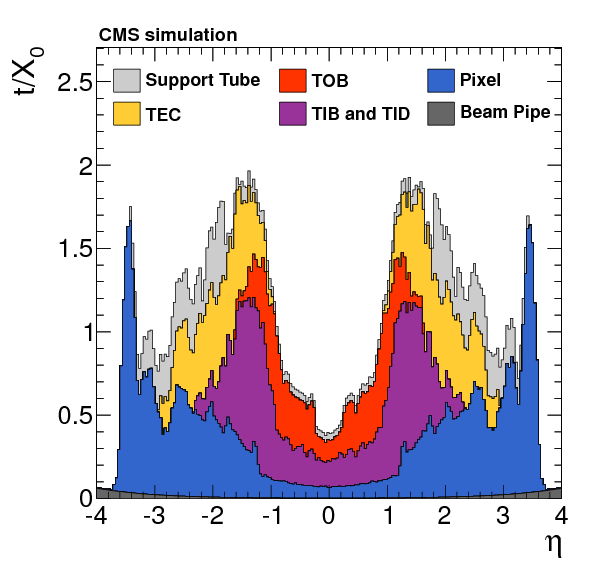
\includegraphics[width=\textwidth]{figures/tracker_material_budget.png}
    \caption[
        Material thickness infront of of ECAL.
    ]{
        The thickness of material, $t$, divided by the radiation length,
        \radiationlength, encountered by particles leaving the nominal
        interaction point before reaching ECAL.
    }
    \label{fig:tracker_material}
\end{figure}

The reconstruction of electrons with $\pt > 20 \GeV$ in CMS begins with a
``seed'' cluster of energy deposits in ECAL \cite{eg_reco_2010}. As an electron
bends in the magnetic field, it takes a helictical path at constant $\eta$ but
changing $\phi$. Any photons radiated by the electron will lie along this path.
These photons must be added together with the electron in order to accurately
measure its energy, and so additional clusters on the same path as the seed
cluster are connected to form a ``supercluster'' \cite{baffioni_2007}. A
supercluster, therefore, includes the energy deposit from the electron as well
as the energy from its nearby photons at constant $\eta$.

From these superclusters, a volume in the tracker where the electron is likely
to have come from is determined by propagating the energy-weighted mean
position of the supercluster back through the magnetic field. This spot is then
used to seed a track-finding algorithm in the pixel layer. Hits in the tracker
are searched for starting at the innermost layer and working outward. In order
to account for the changing shape of the track as the electron loses energy
from interacting with the tracker material, a ``Gaussian Sum Filter'' (GSF)
\cite{adam_2005} is used rather than the simpler Kalman filter used for muons
and hadrons. Low energy electrons ($\ET < 15 \GeV$) are constructed with \pt
from the tracker and \ET from ECAL. For higher energy electrons, the ECAL
energy is used without the tracker \pt to avoid issues introduced by the
possible poor fits in the tracker. The $\eta$ and $\phi$ of all electron
candidates, regardless of energy, is taken from the track by projecting back to
the interaction point.

\section{Additional Corrections}
\label{sec:corrections}

Although the measurement of \phistar is relatively insensitive to the energy of
the electrons, the energy still plays a role in determining the electron \pt
and hence whether an event passes the selection criteria used in this analysis
(discussed in \SEC~\ref{ssec:electron_selection}). Therefore, it is important
to accurately measure this quantity, even if it does not directly change the
final observable. To this end, two sets of energy and momentum corrections,
centrally produced by the CMS collaboration, are applied to both the
data and the reconstructed MC quantities. A summary of the method used to
derive these corrections follows because the papers detailing them are not
public.

\subsection{Regression}

The first set of corrections were calculated using a multivariate regression
trained on \Ztoee and \higgstoZZ MC \cite{cms_an_2012-327}. The regression used
a boosted decision tree trained on 41 different variables parameterizing
electron shower shape, the electron track, and the location of the shower in
EB. The algorithm was trained separately for EB and EE electrons. In order to
prevent over-training the MC samples were split in half, with one half used for
training and the other half used for validation. Electrons used in the
regression were required to have low radiated energy fraction ($< 0.01$) as
determined by the generator level MC and $\pt > 7 \GeV$. The target variable
was the ratio of the generator level \bare electron energy over the
reconstructed energy. This correction was applied to both the data and the
reconstructed MC electrons used in this analysis.

\subsection{Energy Scale and Resolution}

The second set of corrections were calculated with \Ztoee MC using two
independent methods \cite{cms_an_2013-253}. The first method was used to
correct for the energy scale while the second method was used to correct for
the resolution.

In the first method, the MC sample and the data were fit with the convolution
of a Breit-Wigner with a Crystal Ball (CB) function. The CB function is used to
model the resolution of the detector and losses due to bremsstrahlung from the
material in front of ECAL. It consists of a Gaussian with a power-law low-side
tail. It was first used by the Crystal Ball Collaboration \cite{oreglia_1980}.
The Breit--Wigner function models the analytic shape predicted for the \Z mass
resonance. The parameters of the Breit--Wigner were fixed to the nominal values
from the Particle Data Group: $\MZ = 91.188 \GeV$, $\GammaZ = 2.495 \GeV$. The
parameters of the CB function were free parameters in the fit.

The scale correction is both time dependent and $\eta$ dependent and so fits
were performed separately in four pseudorapidity bins in various run ranges.
The peak of the CB function in data and MC were compared with the relative
shift taken as the scale correction, $\Delta P$, given by
\EQ~\ref{eq:scale_correction}.

\begin{equation} \label{eq:scale_correction}
    \Delta P = \frac{\Delta m_{\text{data}} - \Delta m_{\text{MC}}}{\MZ}
\end{equation}

In the second method, two categories of electrons are defined: showering
electrons ($\RNine < 0.94$) and non-showering electrons ($\RNine > 0.94$).
\RNine is the ratio of energy in the \threebythree square of crystals in ECAL
where the electron impacted over the energy in the supercluster and so a larger
number means a narrower shower. A probability density function (PDF) is created
using the \Ztoee MC. For each event in the PDF, the supercluster energy is
modified by applying a Gaussian multiplicative factor $1+\Delta P$ with a
standard deviation of $\Delta \sigma$, where $\Delta P$ is the scale correction
and $\Delta \sigma$ models the resolution. The resolution parameter was
selected for each of the two types of electrons, the four pseudorapidity bins,
and various run ranges using a likelihood maximization. In the EB
pseudorapidity bins, there were enough events to bin in \ET and so these
corrections are also \ET dependent.

\section{Cut Based Identification}
\label{sec:cut_based_id}

There are several centrally-defined ``cut based identification'' requirements
used to select high quality electrons at CMS. These requirements make use of
the variables defined in \SEC~\ref{sec:electron_variables} in order to
reject low quality and unisolation electrons. We use two of requirements,
referred to as \EGMEDIUM and \EGTIGHT, with \EGTIGHT having stricter
requirements than \EGMEDIUM. The exact definition of these requirements are
given in
\TAB~\ref{table:eg_cuts}.

% table:eg_cuts
\begin{table}[h]
    \centering
    \spacerows{1.2}
    \begin{center}
        \begin{tabular}{@{}l r r r r r@{}}
            \toprule
            \multirow{2}{*}{Variable}     & \multicolumn{2}{c}{\EGTIGHT} & \phantom{abc}   & \multicolumn{2}{c}{\EGMEDIUM} \\
            \cmidrule{2-3}
            \cmidrule{5-6}
            & \multicolumn{1}{c}{EB} & \multicolumn{1}{c}{EE} && \multicolumn{1}{c}{EB} & \multicolumn{1}{c}{EE} \\
            \midrule
            $\detain <$                   & 0.004     & 0.005     && 0.004     & 0.007 \\
            $\dphiin <$                   & 0.03      & 0.02      && 0.06      & 0.03 \\
            $\sigmaietaieta <$            & 0.01      & 0.03      && 0.01      & 0.03 \\
            $\HOverE <$                   & 0.12      & 0.10      && 0.12      & 0.10 \\
            $\dzero <$                    & 0.02      & 0.02      && 0.02      & 0.02 \\
            $\dz <$                       & 0.1       & 0.1       && 0.1       & 0.1 \\
            $|\ooeoop| <$                 & 0.05      & 0.05      && 0.05      & 0.05 \\
            $\pvtx <$                     & $10^{-6}$ & $10^{-6}$ && $10^{-6}$ & $10^{-6}$ \\
            $\nmiss \le$                  & 0         & 0         && 1         & 1 \\
            $\PFISO <$                    & 0.10      & 0.10      && 0.15      & 0.15 \\
            \bottomrule
        \end{tabular}
    \end{center}
    \caption[
        Identification and isolation requirements for \EGTIGHT and \EGMEDIUM.
    ]{
        Identification and isolation requirements for \EGTIGHT and \EGMEDIUM
        requirements in the ECAL barrel (EB) and ECAL endcap (EE).
    }
    \label{table:eg_cuts}
\end{table}


\section{Electron Variables}
\label{sec:electron_variables}

Not everything reconstructed as an electron in CMS is a real electron. One
source of fake electrons is a process referred to as charge exchange:
$\ChargeExchange \to 2 \photon + \proton$. In this process, a charged pion
interacts with a nuclear neutron which convert to a neutral pion and a proton
where the neutral pion quickly decays to two photons. If this process happens
in ECAL, it can result in a track (from the charged
pion) pointing at a supercluster with a shape similar to a photon or electron
shower (from the two photons) which will often be reconstructed as an electron.
Another source of fake electrons is coincidence events where a photon impacts
ECAL near the track left by another charged particle.

Not every electron is equally likely to be from a \Ztoee decay; many electrons
detected in CMS come from other processes. One such process is photon
conversion, \PhotonConversion, where a photon in the presence of a nucleus
converts to two electrons. Another source of electrons is from QCD jets which
can sometimes produce an electron in their numerous decays.

There are several electron variables defined in order to allow the separation
of these lower quality and fake electrons from the electrons from \Ztoee
decays. These variables are broken down into three categories:

\begin{description}
    \item[Identification (ID):] \hfill \\
        These variables quantify how much like an electron the reconstructed
        particle looks and are used to reject fake electrons like those from
        charge exchange.
    \item[Conversion Rejection:] \hfill \\
        These variables are used to reject electrons from \PhotonConversion
        conversions.
    \item[Isolation:] \hfill \\
        These variables measures how much energy from other particles is
        deposited near the electron in the detector and are used to help reject
        electrons within jets.
\end{description}

The following subsections contain plots of some of the most important electron
variables as well as a discussion of their use in selecting electrons from
\Ztoee decays. The data shown on the plots consists of every electron candidate
in the \SingleMuon dataset with $|\eta| < 2.4$ and $\pt > 20 \GeV$. This
dataset was used because the trigger that selects events for it makes no
selection on the electron variables and therefore the electron candidates in
the set represent a sample of minimally-biased electrons. The MC electrons are
from the \MADGRAPH \DYtoll sample with the same kinematic requirements are
applied as are used on the data, with the additional requirement that the event
must contain a generator level \Ztoee decay. These selections give us a data
sample that is indicative of the general distribution of all electrons in CMS
events, while the MC sample shows what the distribution looks like in signal
events.

\subsection{Identification}

The shape of the electromagnetic shower in the calorimeters is used to
discriminate between electrons and other particles. Electrons generally have
very narrow showers whereas hadronic particles have wide showers. The size of
the shower in $\eta$ is characterized by \sigmaietaieta. Charge exchange events
often have a higher \sigmaietaieta than real electrons because the proton is
can be knocked loose by the interaction and leaves a broader shower.
Comparisons of the \sigmaietaieta distributions between all electrons and for
signal electrons for both EB and EE are shown in \FIG~\ref{fig:sieie}.

\begin{figure}[!htbp]
    \centering
    \begin{subfigure}[b]{\StackedPlotWidth}
        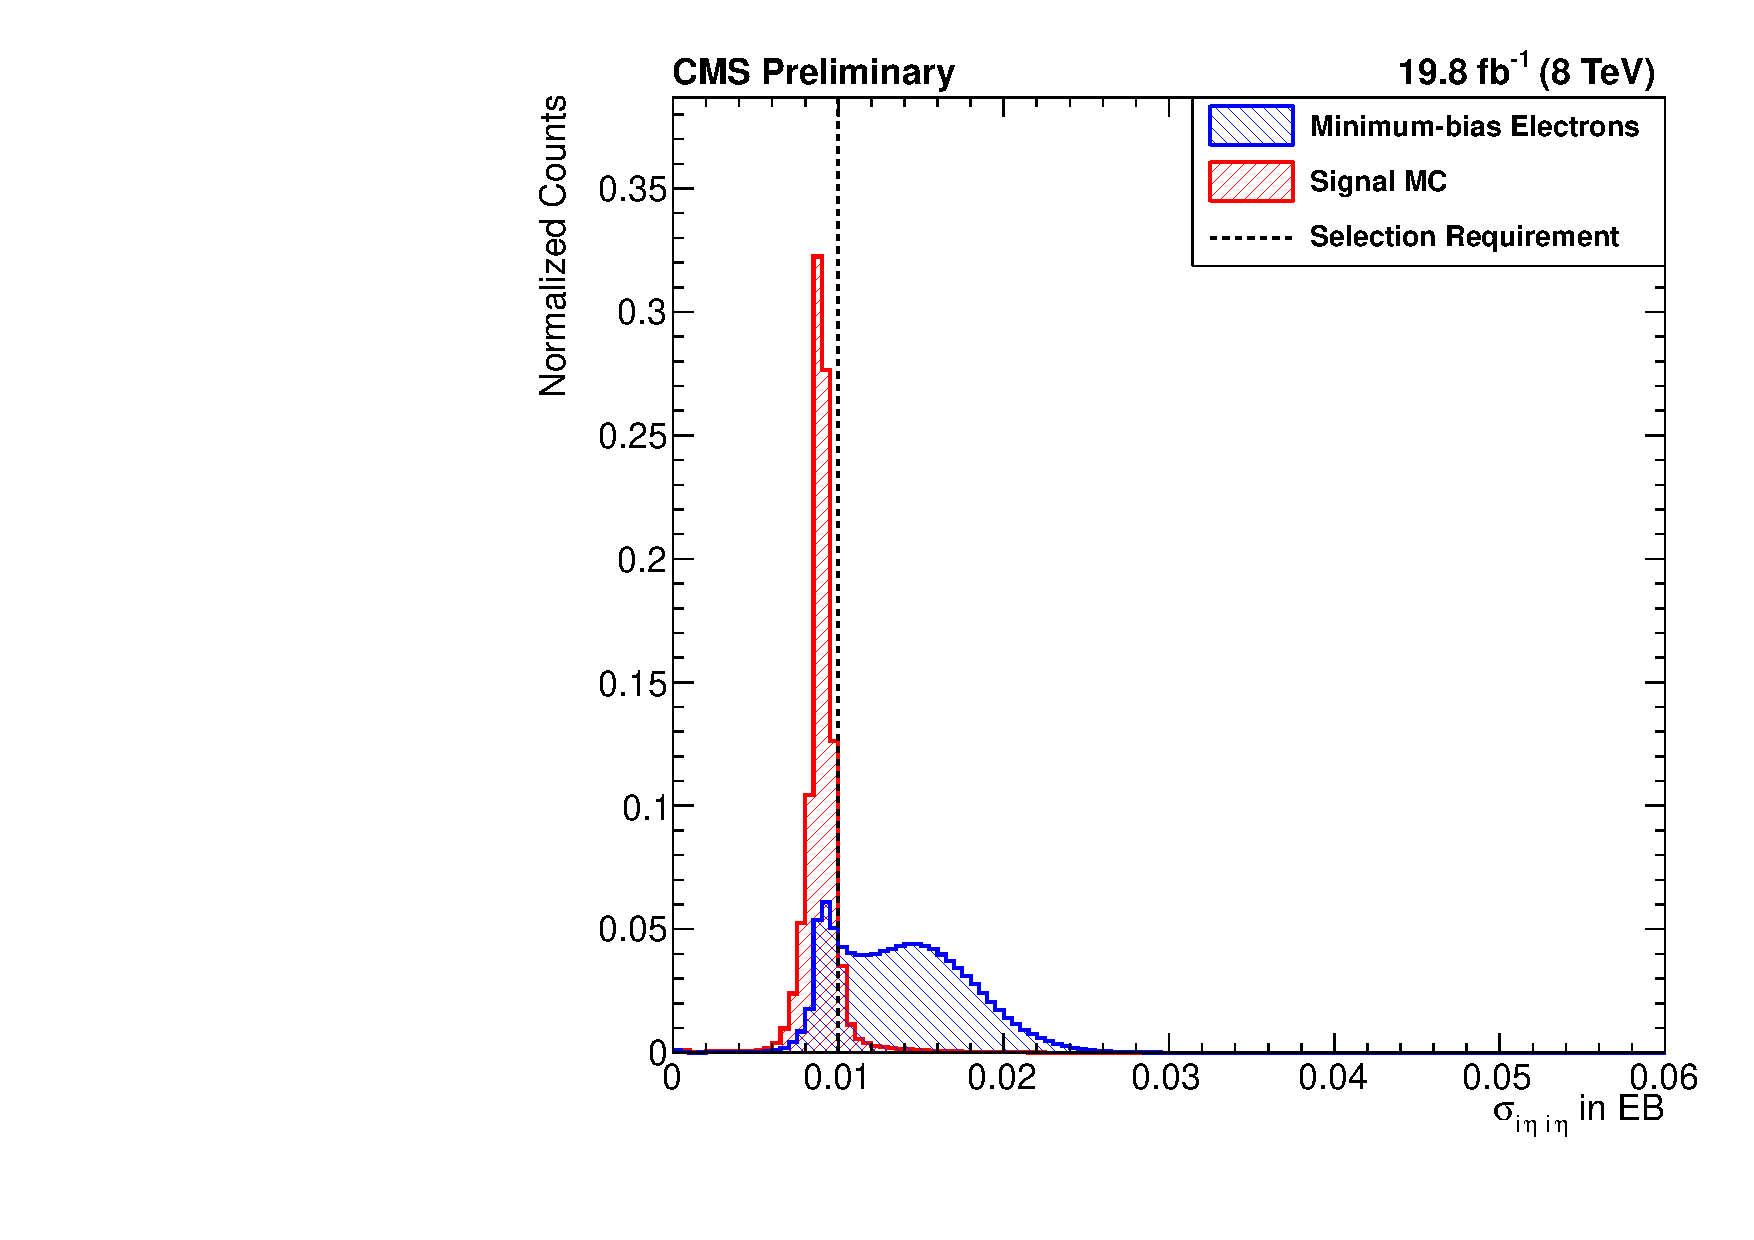
\includegraphics[width=\textwidth]{figures/e_reco_var_sigma_ieta_ieta_eb.pdf}
        \caption{}
        \label{fig:sieie_eb}
    \end{subfigure}
    \begin{subfigure}[b]{\StackedPlotWidth}
        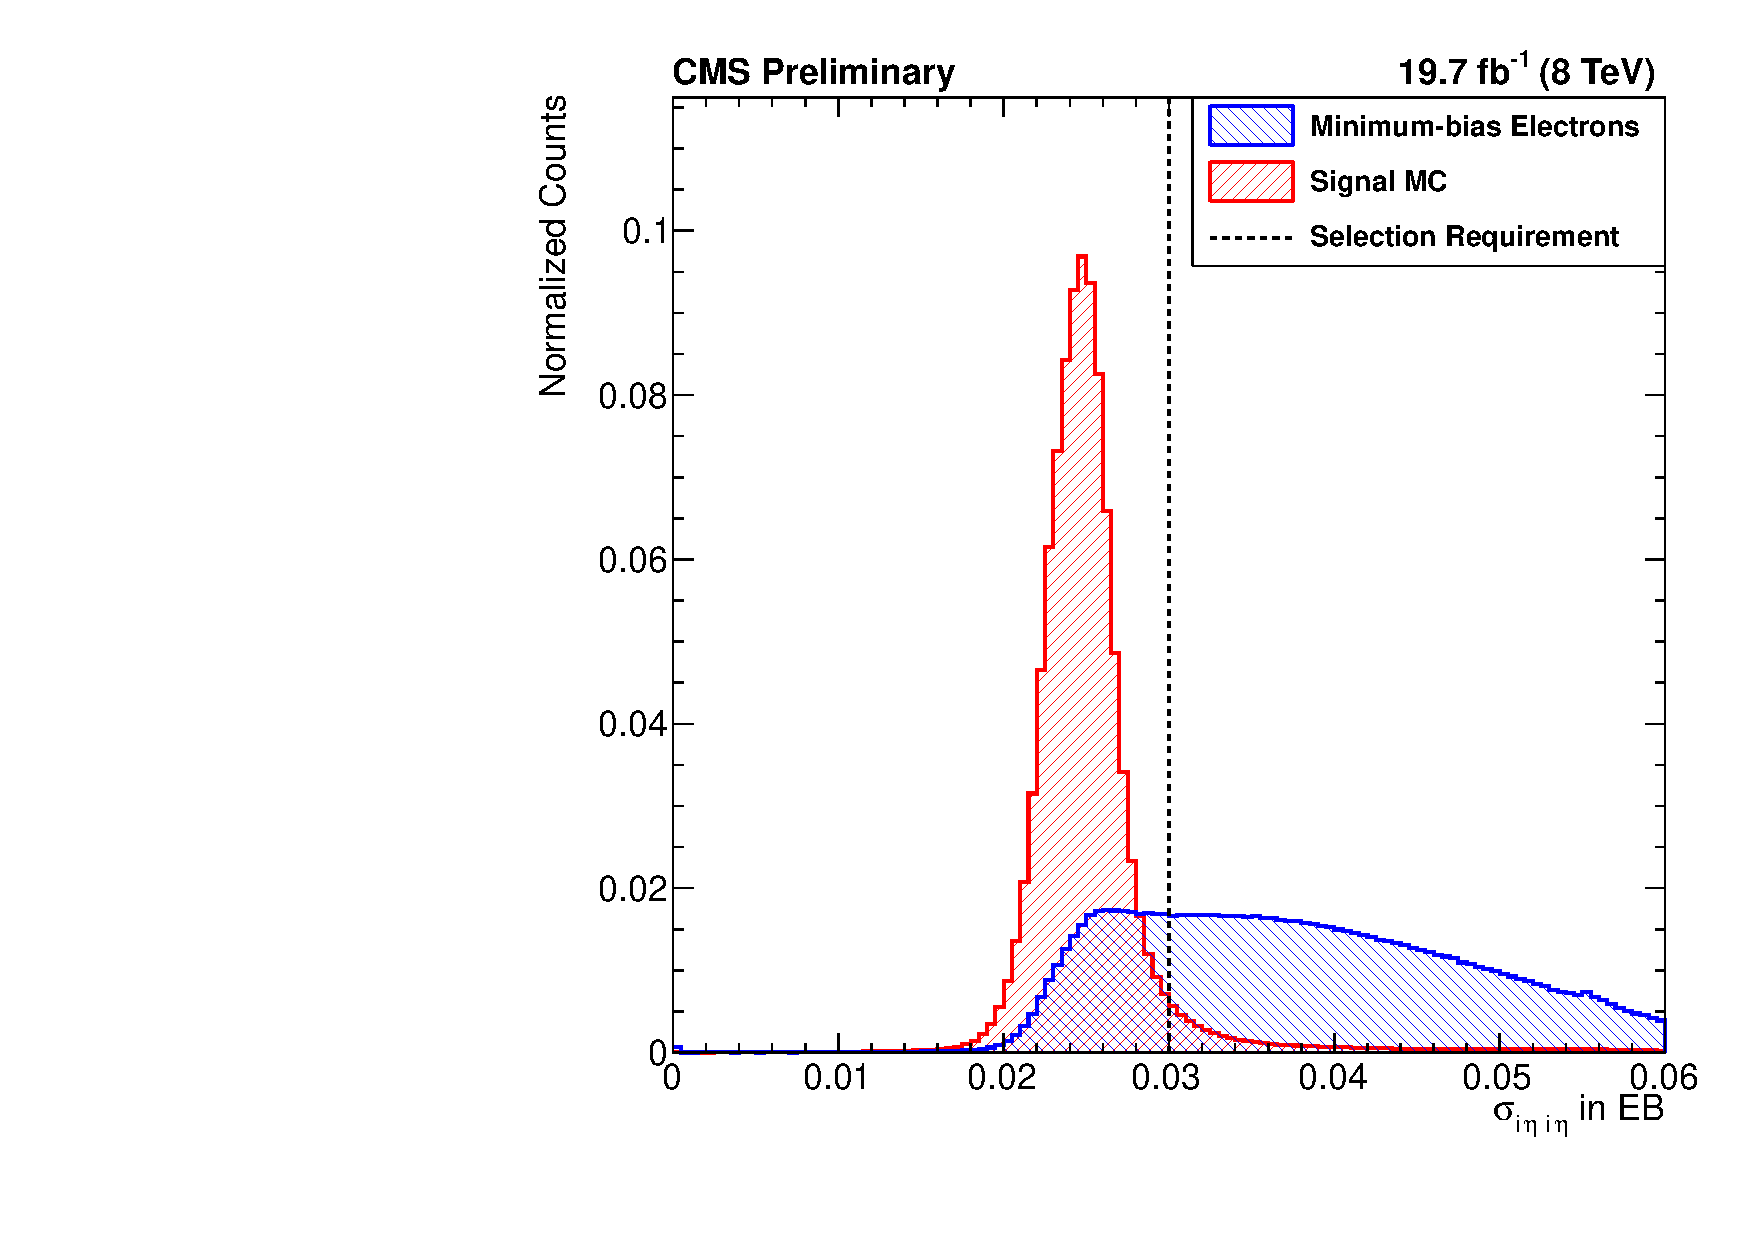
\includegraphics[width=\textwidth]{figures/e_reco_var_sigma_ieta_ieta_ee.pdf}
        \caption{}
        \label{fig:sieie_ee}
    \end{subfigure}
    \caption[
        Distributions of $\sigmaietaieta$ in EB and EE in data and MC.
    ]{
        The $\sigmaietaieta$ variable distribution in EB (top) and EE (bottom)
        for all electrons with $\pt > 20 \GeV$ and $|\eta| < 2.4$ in a set of
        events selected with a muon trigger and in \MADGRAPH \Ztoee MC.
    }
    \label{fig:sieie}
\end{figure}

Electron showers are mostly contained within ECAL and so the ratio of energy
around the hit in HCAL over the energy around the hit in ECAL, \HOverE, is also
used to parameterize the shower shape. Charge exchange events often have higher
\HOverE than electrons because the loose proton can escape and enter HCAL. A
comparison of the \HOverE distributions between all electrons and for signal
electrons is shown in \FIG~\ref{fig:he}.

\begin{figure}[!htbp]
    \centering
    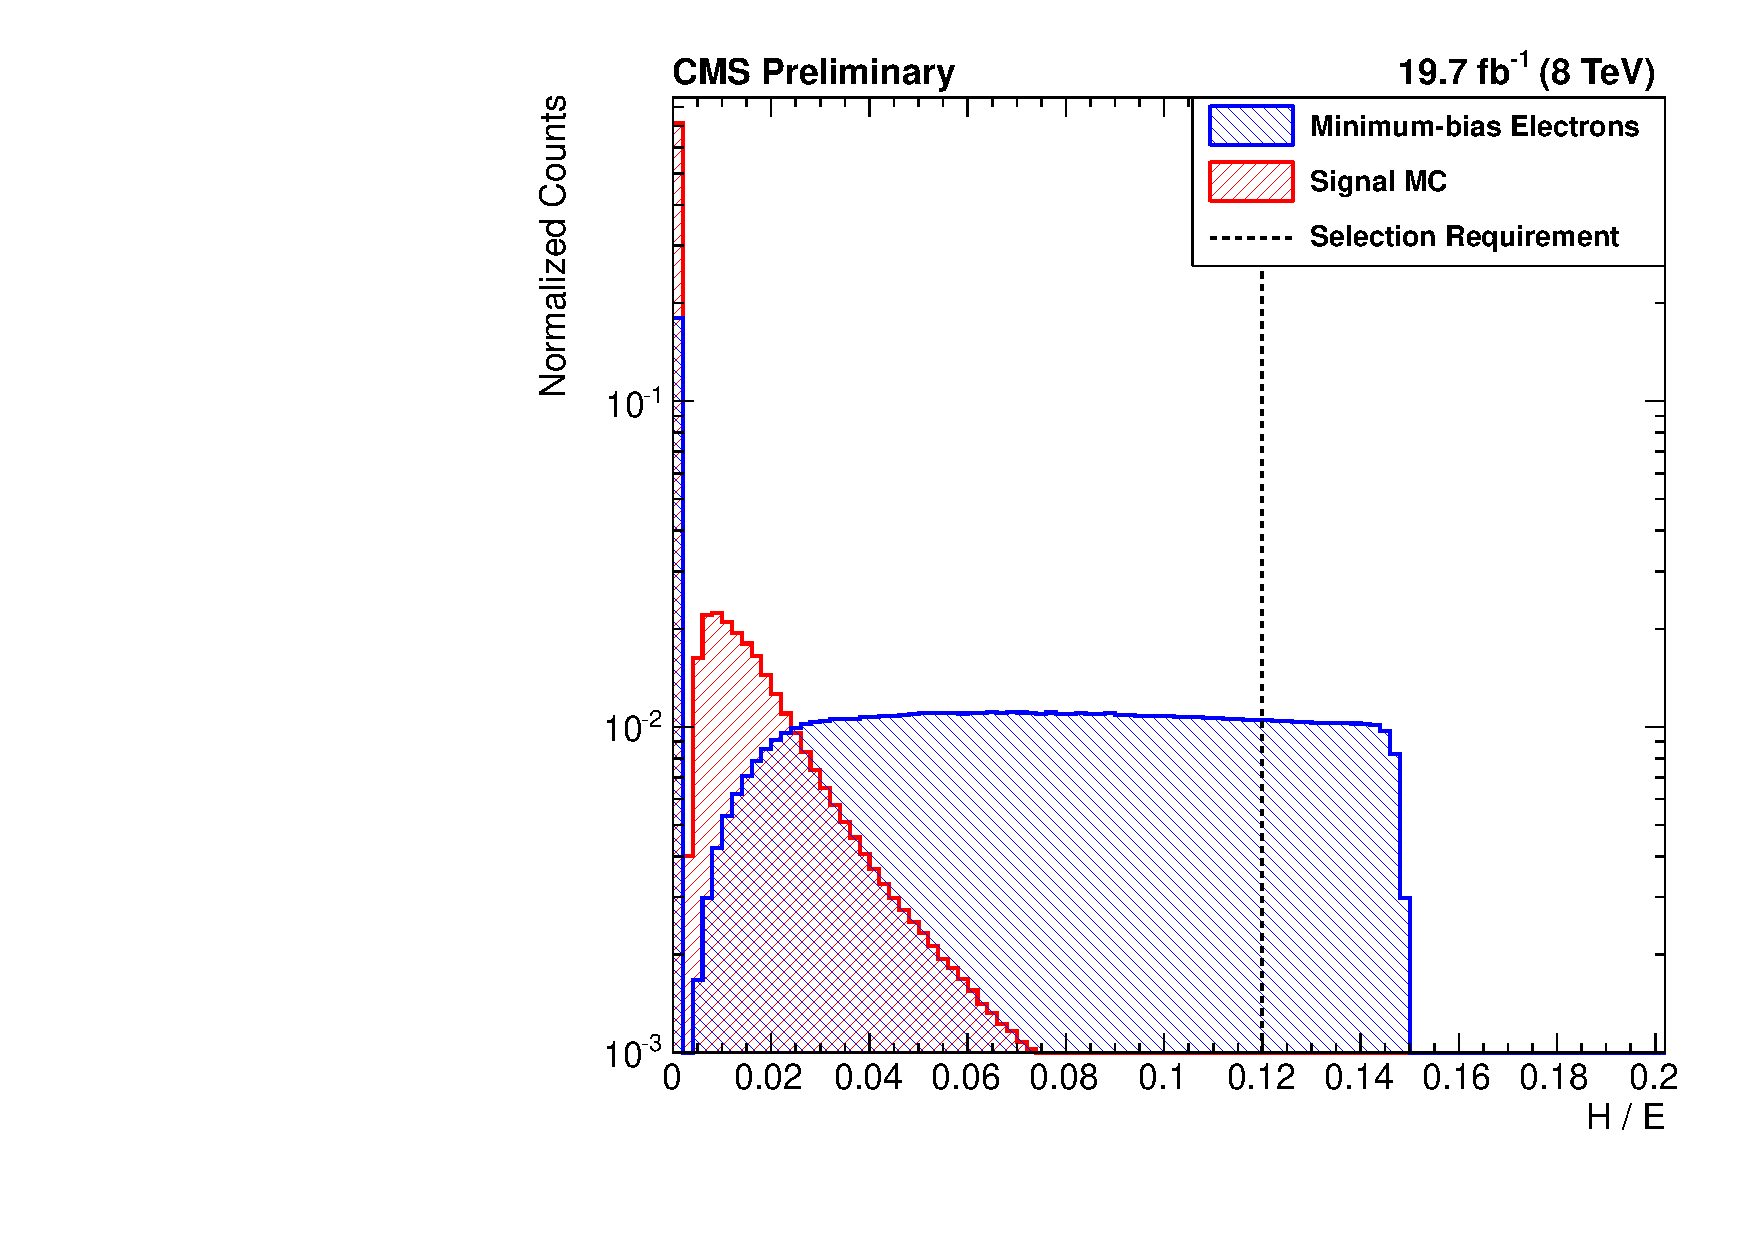
\includegraphics[width=\StackedPlotWidth]{figures/e_reco_var_he.pdf}
    \caption[
        Distributions of \HOverE in data and MC.
    ]{
        The \HOverE distributions for all electrons with $\pt > 20 \GeV$ and
        $|\eta| < 2.4$ in a set of events selected with a muon trigger and in
        \MADGRAPH \Ztoee MC.
    }
    \label{fig:he}
\end{figure}

The distance between the track and the supercluster in \coordetaphi space is
given by \dphiin and \detain. Real electrons have small values of \dphiin and
\detain because the electron caused both the track and the supercluster, but
coincidence events are equally as likely to have a large track separation as a
small one because each element comes from an independent object. Comparisons of
the \dphiin and \detain distributions between all electrons and for signal
electrons are shown in \FIGS~\ref{fig:deta} and \ref{fig:dphi}, respectively.

\begin{figure}[!htbp]
    \centering
    \begin{subfigure}[b]{\StackedPlotWidth}
        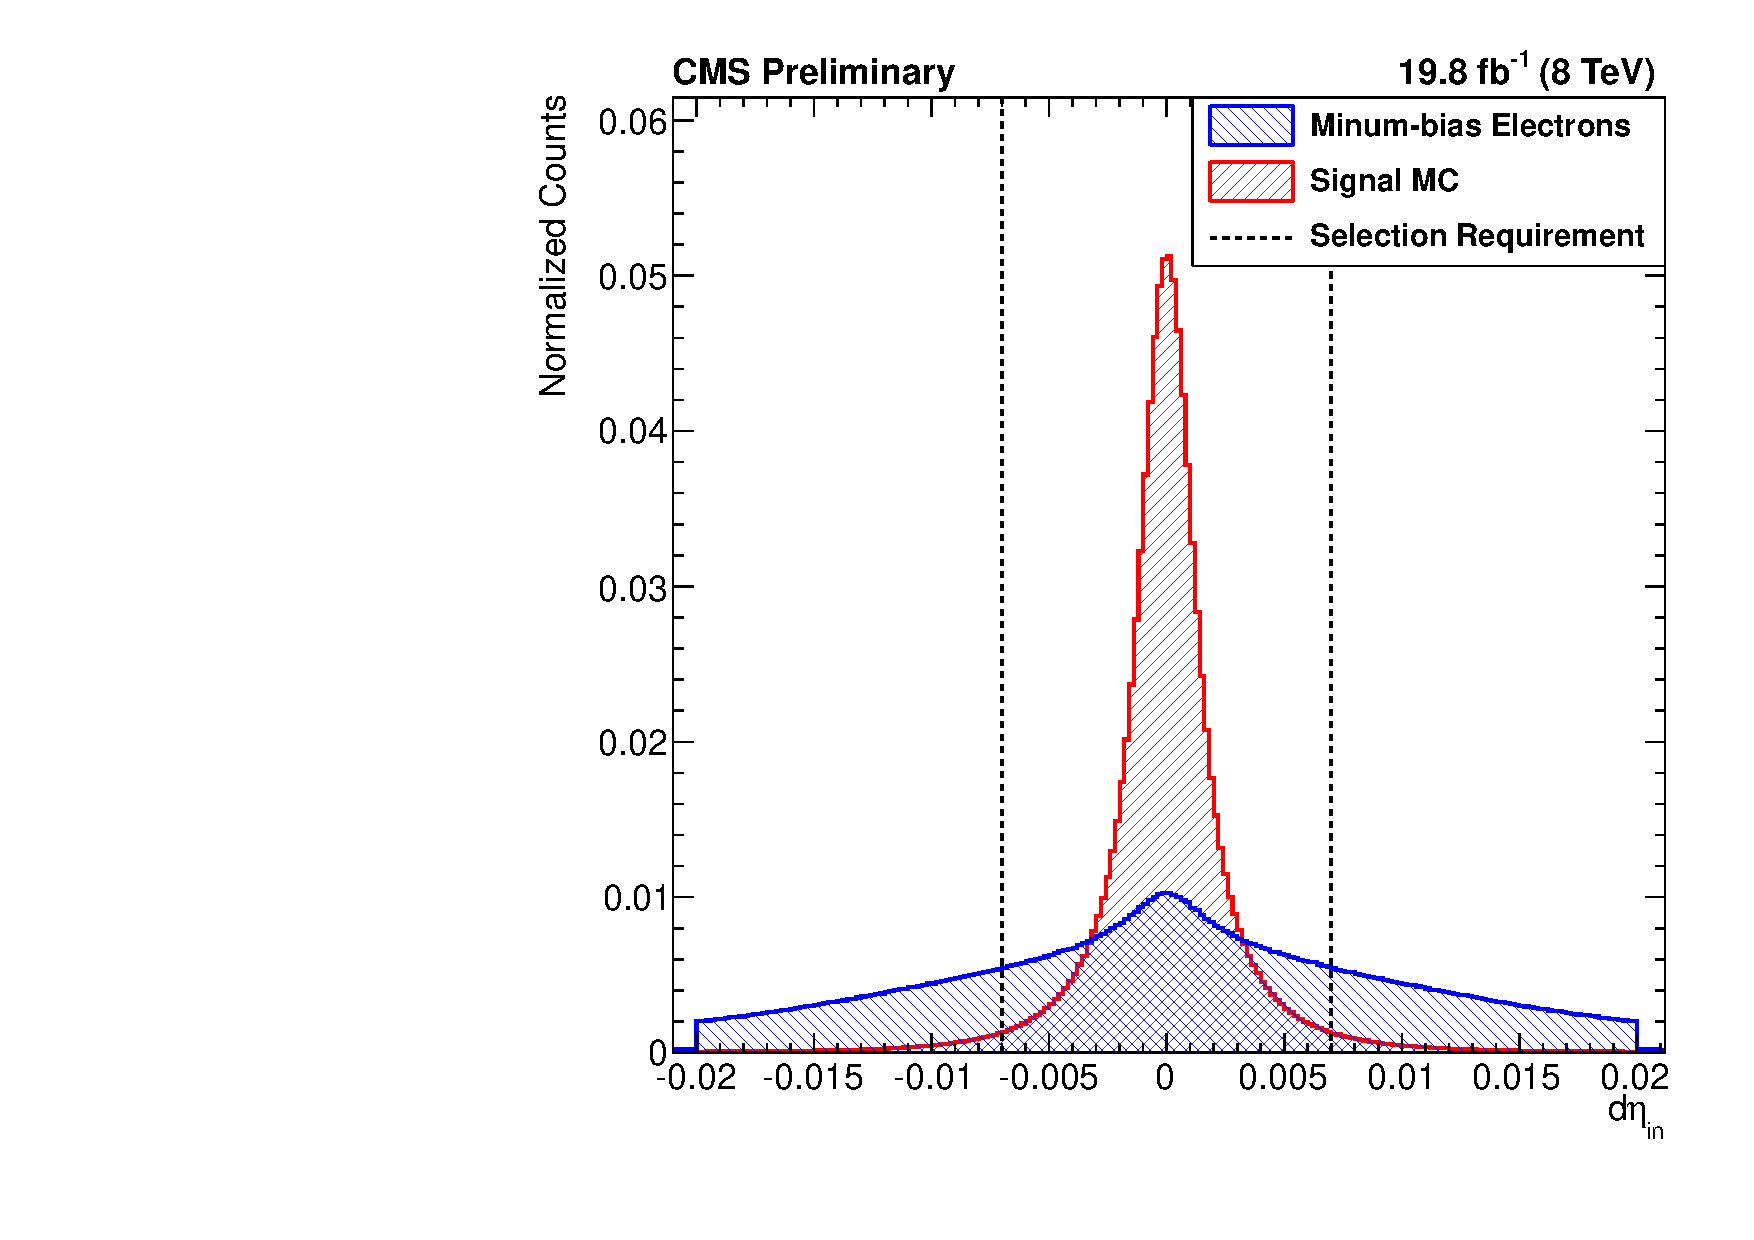
\includegraphics[width=\textwidth]{figures/e_reco_var_deta.pdf}
        \caption{}
        \label{fig:deta}
    \end{subfigure}
    \begin{subfigure}[b]{\StackedPlotWidth}
        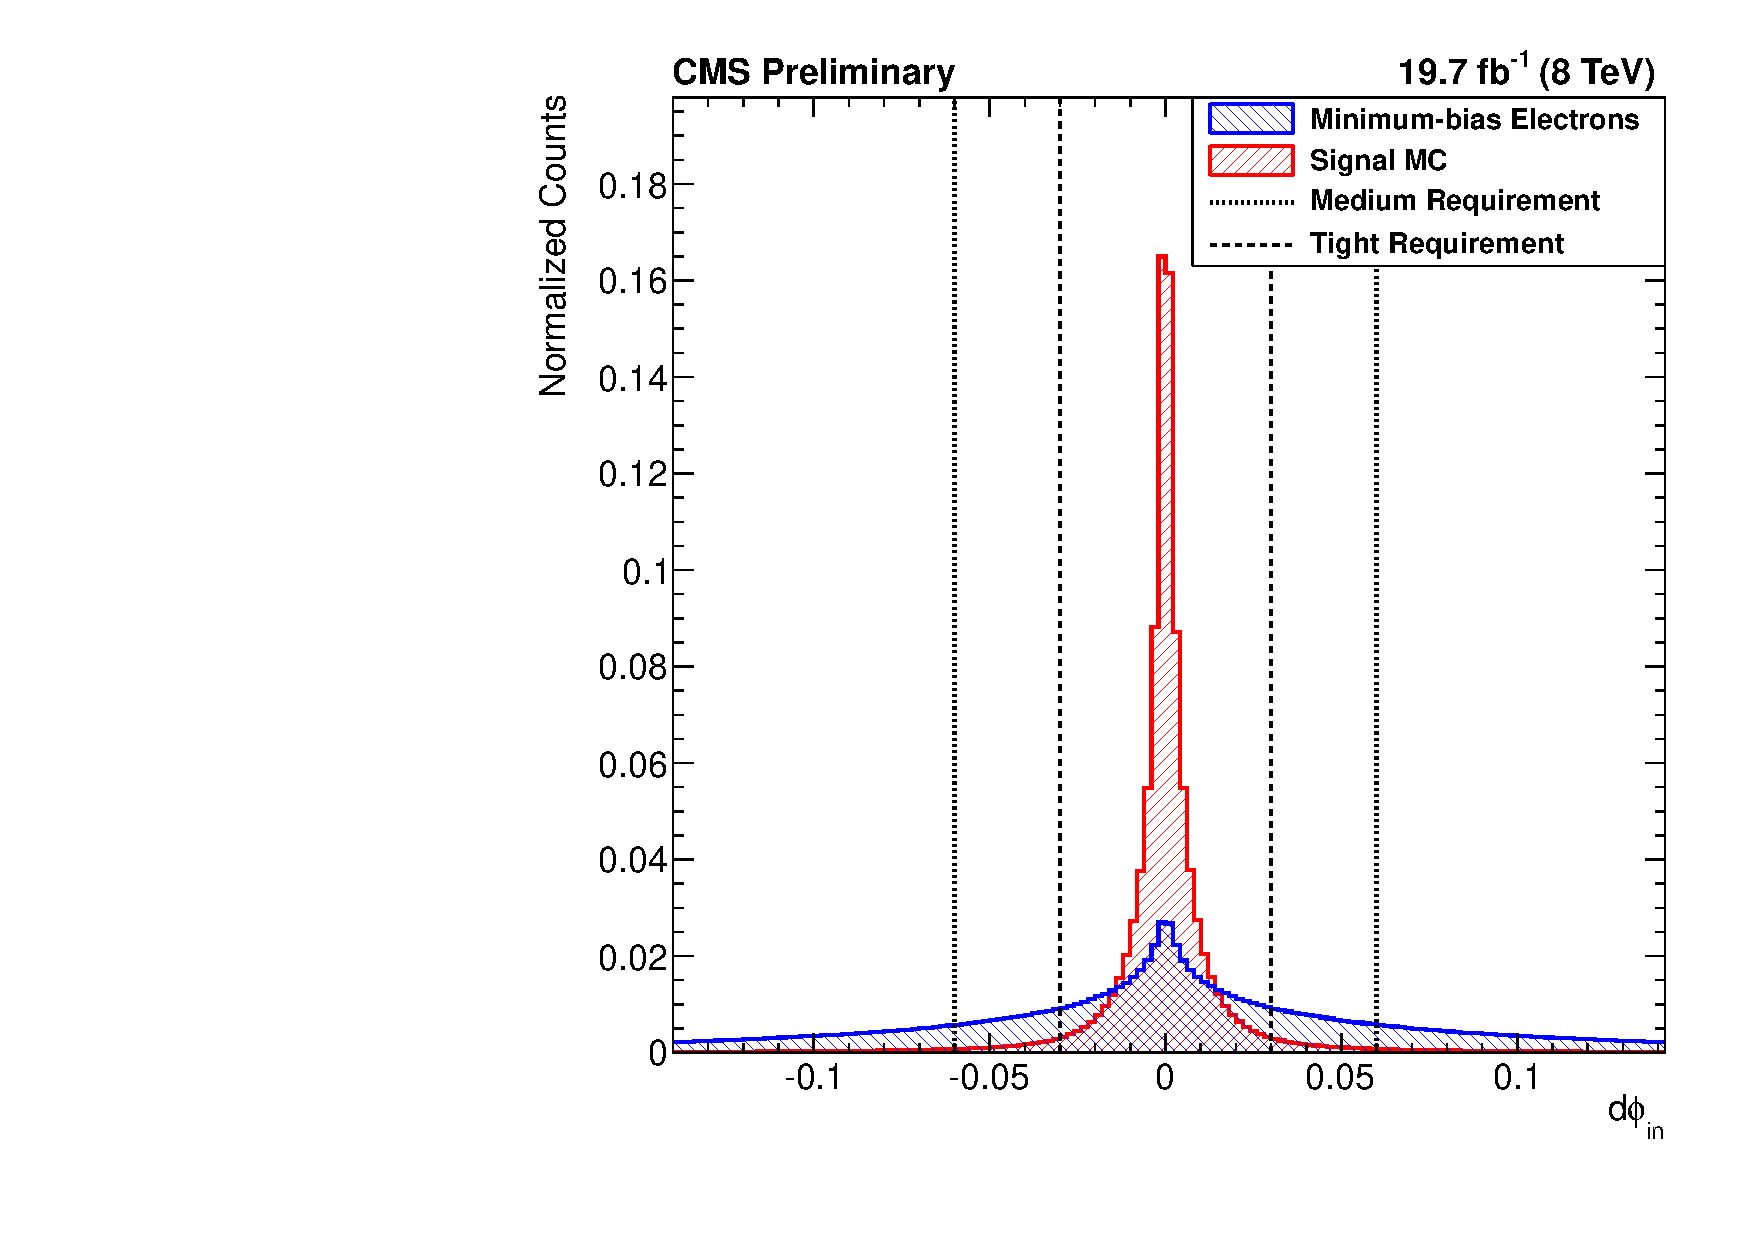
\includegraphics[width=\textwidth]{figures/e_reco_var_dphi.pdf}
        \caption{}
        \label{fig:dphi}
    \end{subfigure}
    \caption[
        Distributions of $\detain$ and $\dphiin$ in data and MC.
    ]{
        The $\detain$ (top) and $\dphiin$ (bottom) variable distributions for
        all electrons with $\pt > 20 \GeV$ and $|\eta| < 2.4$ in a set of
        events selected with a muon trigger and in \MADGRAPH \Ztoee MC.
    }
    \label{fig:dtrack}
\end{figure}

The compatibility of energy of the supercluster and the momentum of the track
is parameterized by \ooeoop. Electrons will have \ooeoop near \num{0} because
their momentum and energy, having been measured for the same object, will
agree. Charge exchange events will have positive \ooeoop as their momentum is
measured in the tracker before the interaction (and hence measures the full
momentum of the \pionplus) but their energy is measured in ECAL after the
interaction and hence after the proton has carried away some of the energy.
Coincidence events, because the energy and momentum are measured from
independent objects, can take both positive and negative values of \ooeoop. A
comparison of the \ooeoop distributions between all electrons and for signal
electrons is shown in \FIG~\ref{fig:ooeoop}.

\begin{figure}[!htbp]
    \centering
    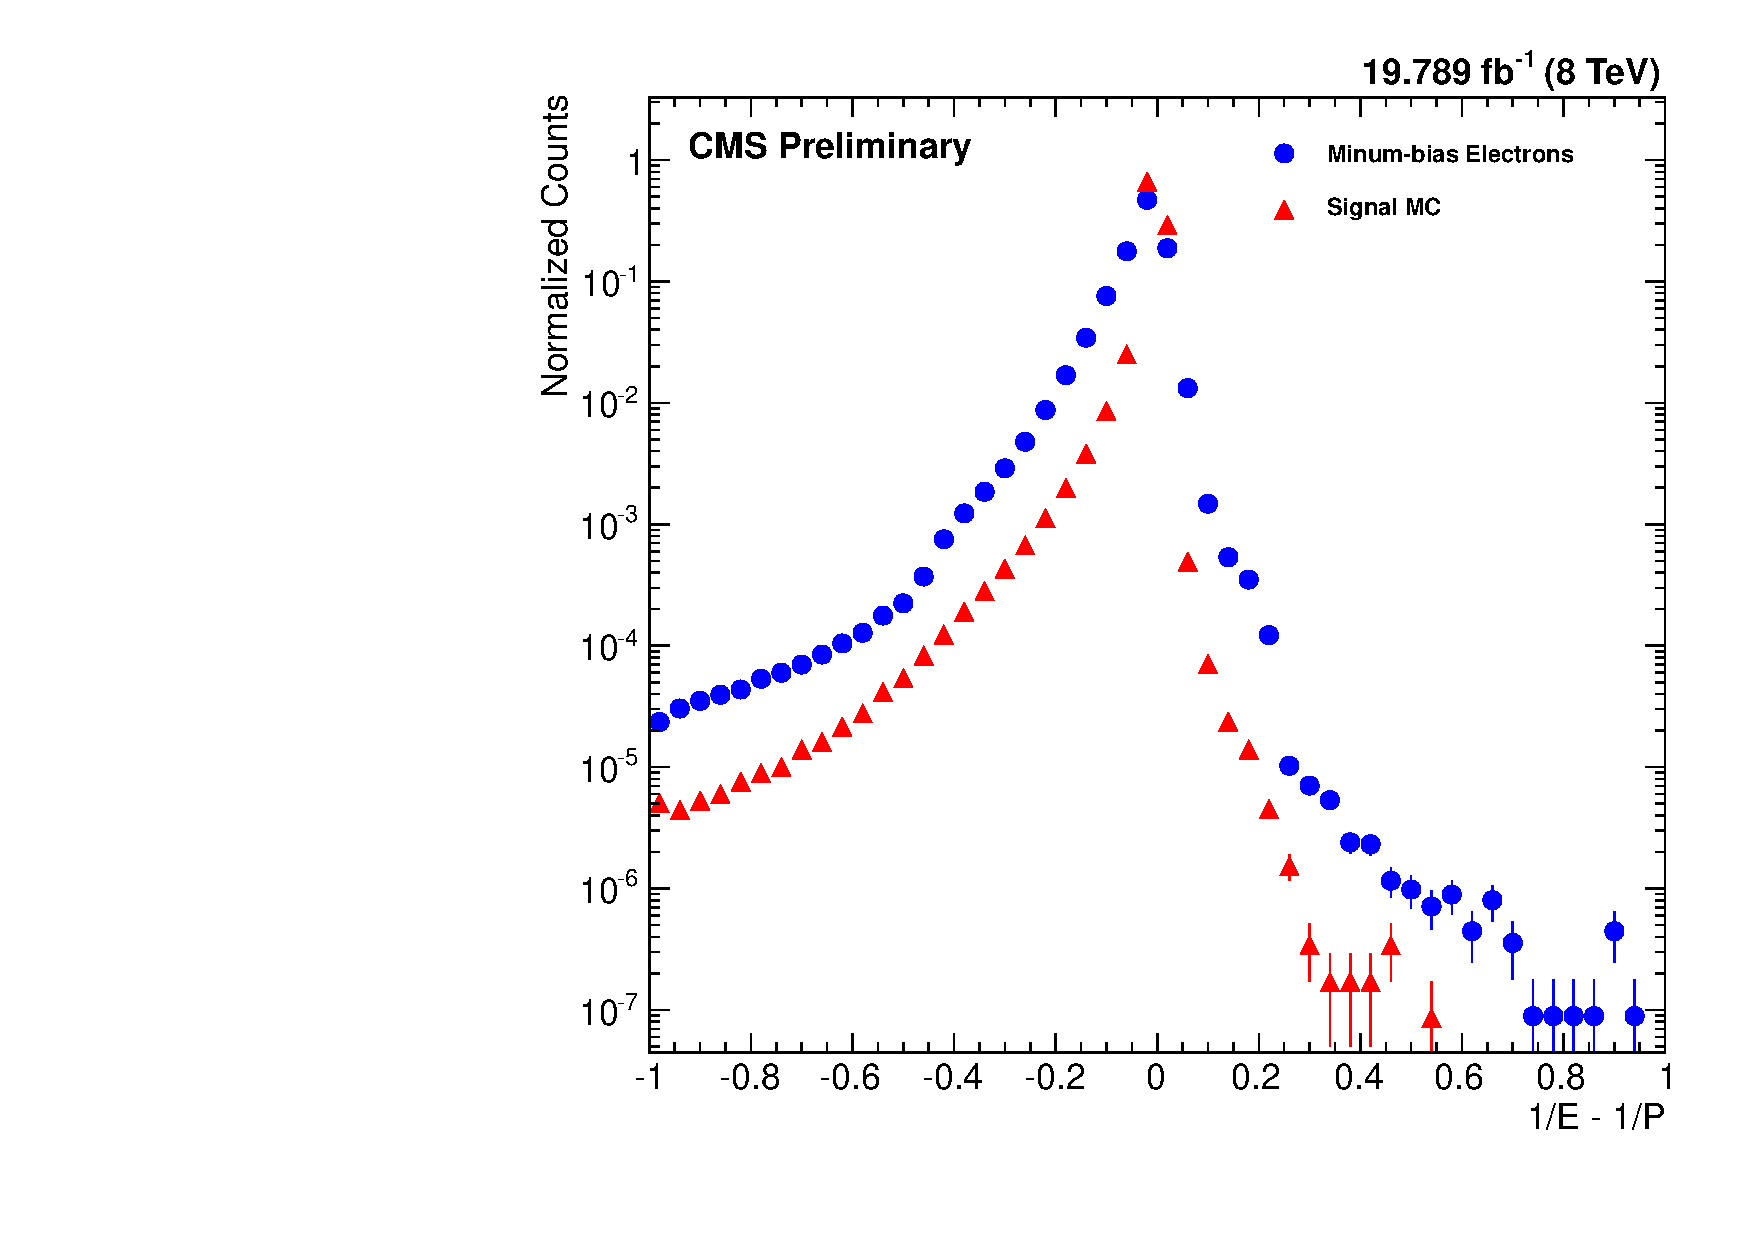
\includegraphics[width=\StackedPlotWidth]{figures/e_reco_var_1oe_1op.pdf}
    \caption[
        Distributions of \ooeoop in data and MC.
    ]{
        The \ooeoop distributions for all electrons with $\pt > 20 \GeV$ and
        $|\eta| < 2.4$ in a set of events selected with a muon trigger and in
        \MADGRAPH \Ztoee MC.
    }
    \label{fig:ooeoop}
\end{figure}

\subsection{Conversion Rejection}

Photon conversions generally happen away from the primary vertex and so the
distances of the hits in the track from the vertex are useful quantities to
reject conversions. The transverse and longitudinal separation between the
track and the primary vertex are given by \dzero and \dz. In addition to
the raw distance of the track from the primary vertex, there is also a fit
probability, \pvtx, which indicates the probability that a track came from the
primary vertex. This variable is also used to reject conversions. Comparisons
of the \dzero and \dz distributions between all electrons and for signal
electrons are shown in \FIGS~\ref{fig:d0} and \ref{fig:dz}, respectively.

\begin{figure}[!htbp]
    \centering
    \begin{subfigure}[b]{\StackedPlotWidth}
        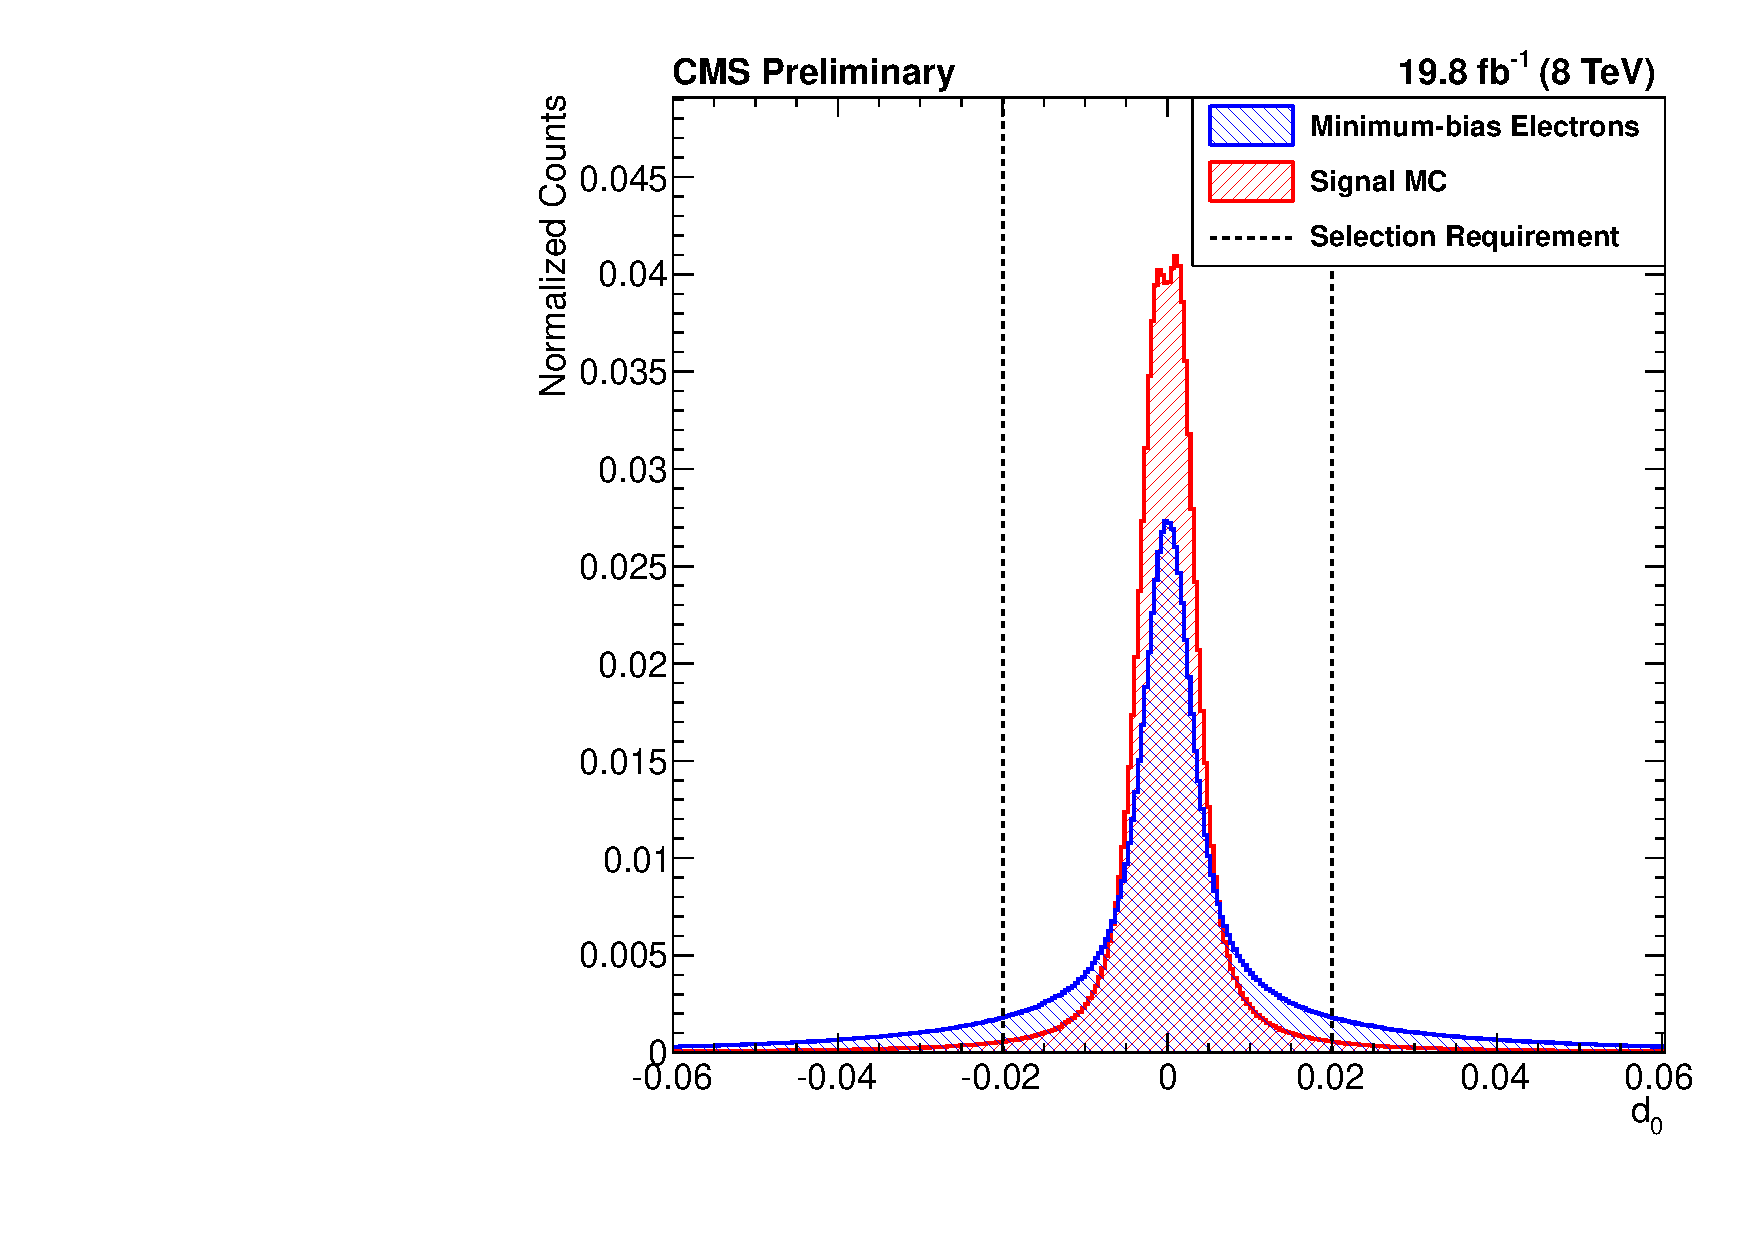
\includegraphics[width=\textwidth]{figures/e_reco_var_d0.pdf}
        \caption{}
        \label{fig:d0}
    \end{subfigure}
    \begin{subfigure}[b]{\StackedPlotWidth}
        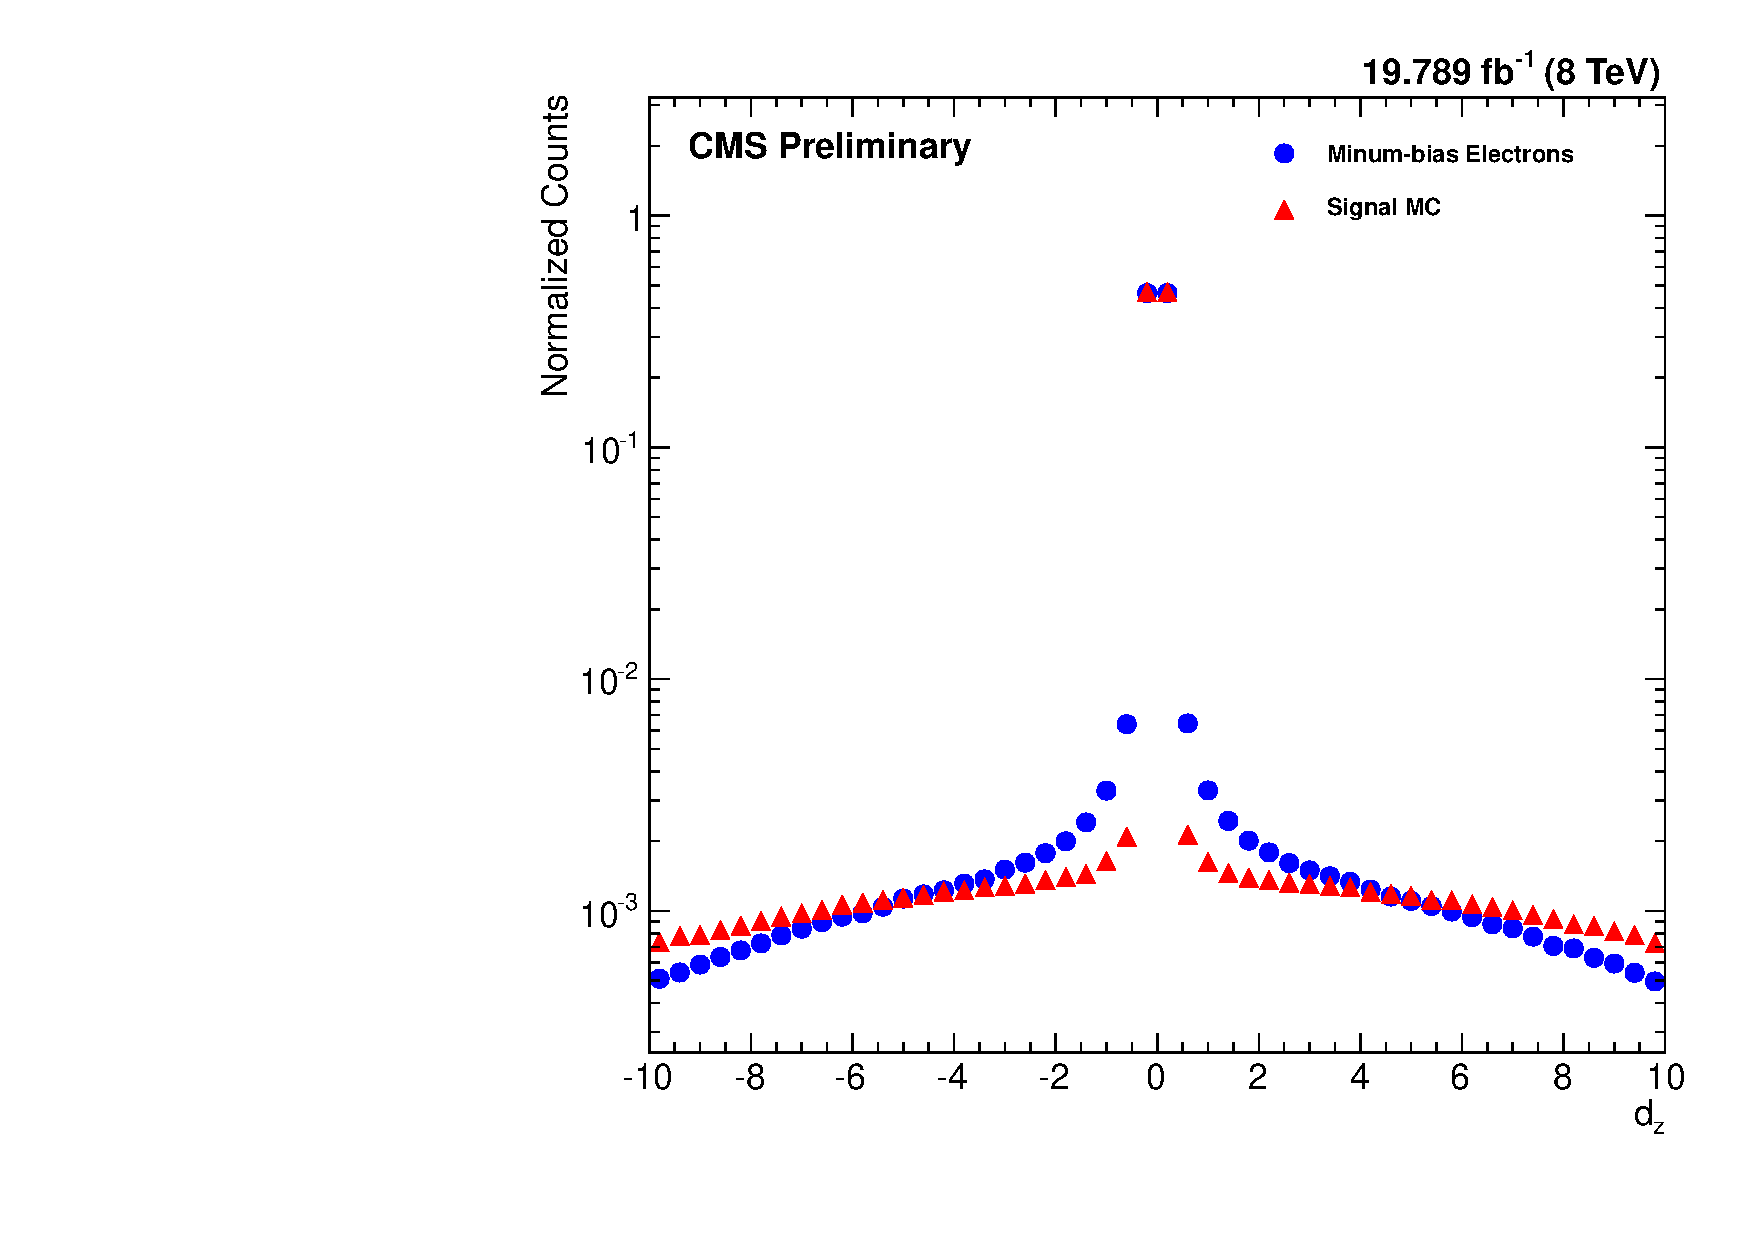
\includegraphics[width=\textwidth]{figures/e_reco_var_dz.pdf}
        \caption{}
        \label{fig:dz}
    \end{subfigure}
    \caption[
        Distributions of \dzero and \dz in data and MC.
    ]{
        The \dzero (top) and \dz (bottom) variable distributions for all
        electrons with $\pt > 20 \GeV$ and $|\eta| < 2.4$ in a set of events
        selected with a muon trigger and in \MADGRAPH \Ztoee MC.
    }
    \label{fig:d0_dz}
\end{figure}

Conversions generally happen after the photon passes through several layers of
the tracker and so their tracks will have missing layers, the number of which
is given by \nmiss. A comparison of the \nmiss distributions between all
electrons and for signal electrons is shown in \FIG~\ref{fig:nmiss}.

\begin{figure}[!htbp]
    \centering
    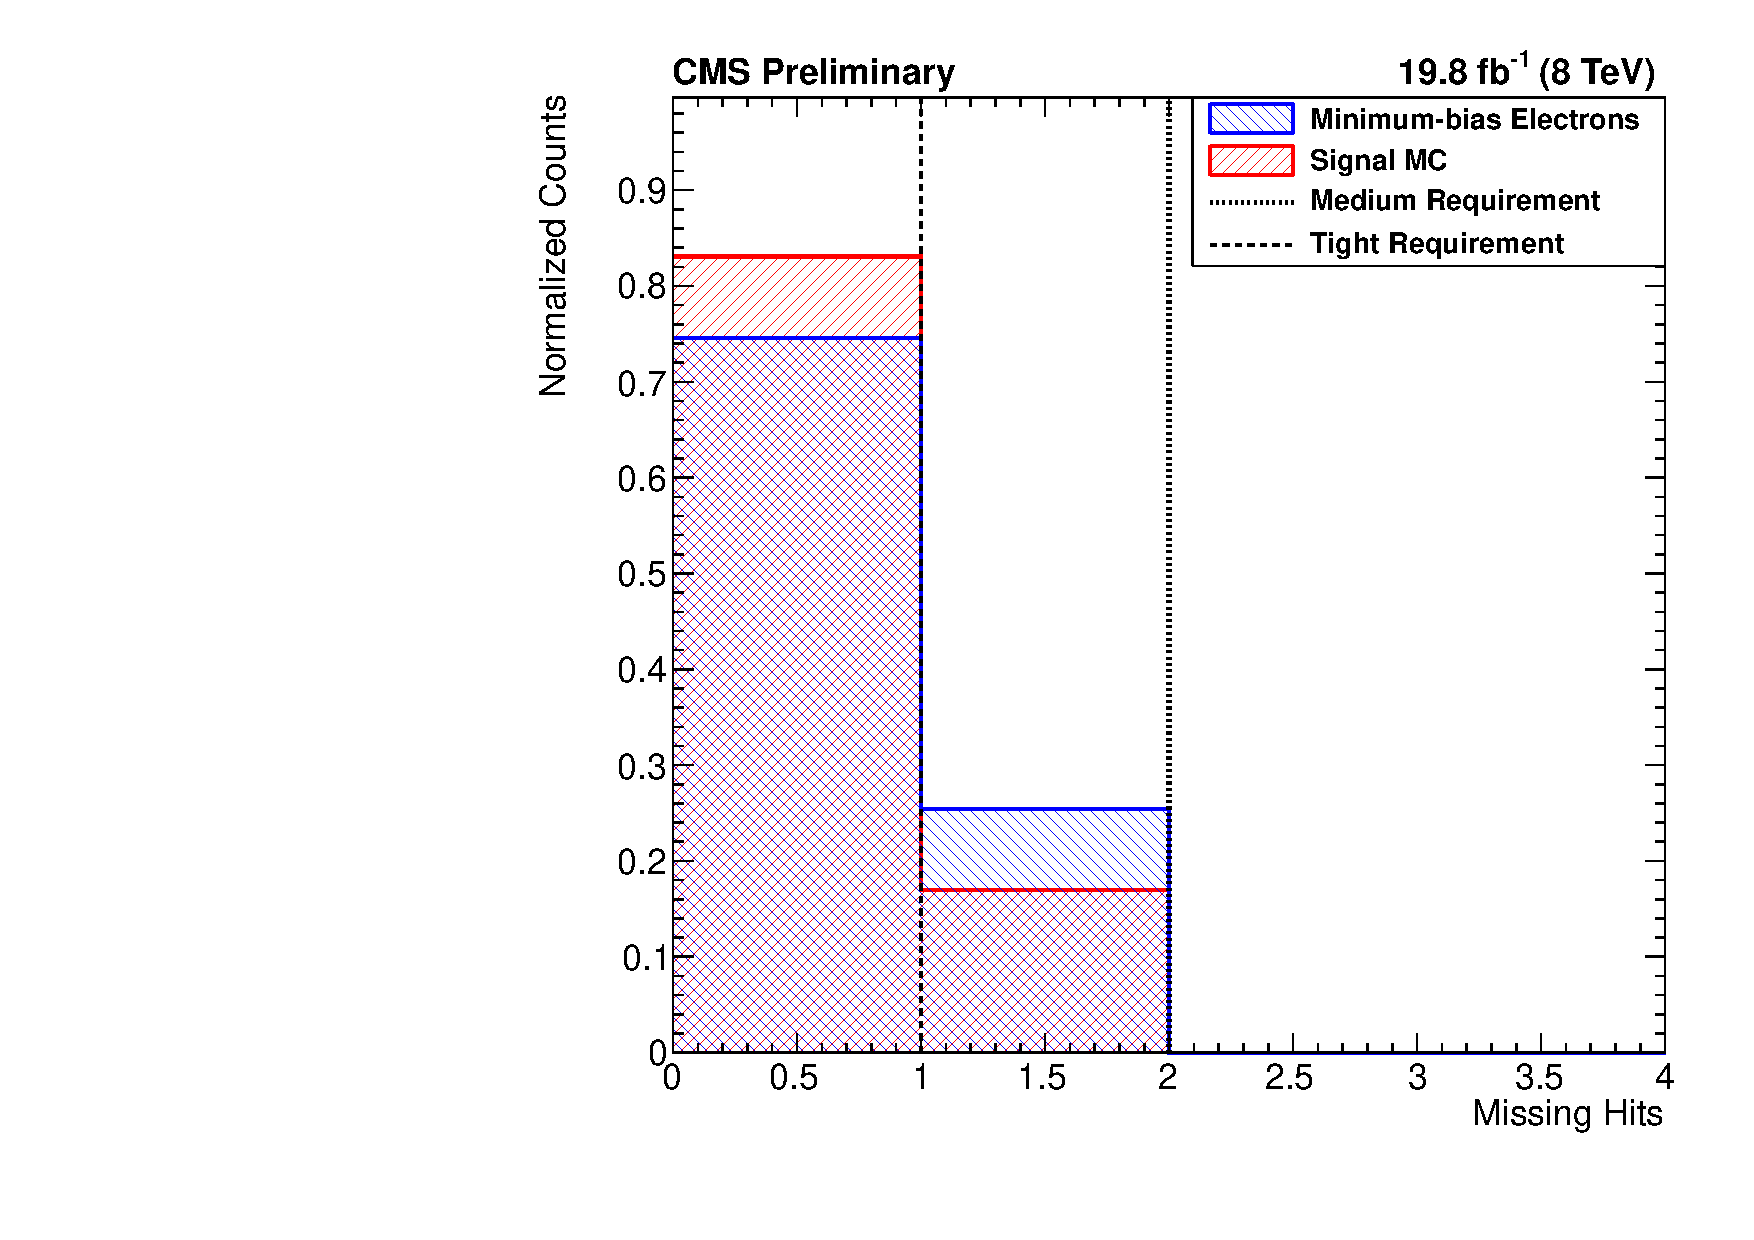
\includegraphics[width=\StackedPlotWidth]{figures/e_reco_var_nmiss.pdf}
    \caption[
        Distributions of \nmiss in data and MC.
    ]{
        The \nmiss distribution for all electrons with $\pt > 20 \GeV$ and
        $|\eta| < 2.4$ in a set of events selected with a muon trigger and in
        \MADGRAPH \Ztoee MC.
    }
    \label{fig:nmiss}
\end{figure}

\subsection{Isolation}

Hadronic jets sometimes produce electrons in the numerous decays happening
within them. These electrons can be rejected by looking at the sum of the
energy in the tracker, ECAL, and HCAL around the electron, as electrons in jets
will have a large amount of energy surrounding them, whereas electrons from \Z
decays will tend to be isolated.

The isolations used in the trigger (\SingleElectronTrigger) are defined as
follows:

\begin{equation}
    \HCALISO = \frac{\DeltaRSum \EHCAL}{\etElectron}
\end{equation}

\begin{equation}
    \ECALISO = \frac{\DeltaRSum \EECAL - \ESC}{\etElectron}
\end{equation}

\noindent where \DeltaRSum is a sum on the energy in a $\Delta R < 0.3$ cone around the
supercluster location, \EHCAL is the energy in HCAL, \EECAL is the energy in
ECAL, and \ESC is the energy of the supercluster, which is subtracted out of
the ECAL isolation sum. No subtraction is applied to the HCAL isolation as we
expect all of the electron's energy to be contained in ECAL. Both isolation
values are normalized by the \et of the electron. Comparisons of the \HCALISO
and \ECALISO distributions between all electrons and for signal electrons are
shown in \FIGS~\ref{fig:hcal_iso} and \ref{fig:ecal_iso}, respectively.

\begin{figure}[!htbp]
    \centering
    \begin{subfigure}[b]{\StackedPlotWidth}
        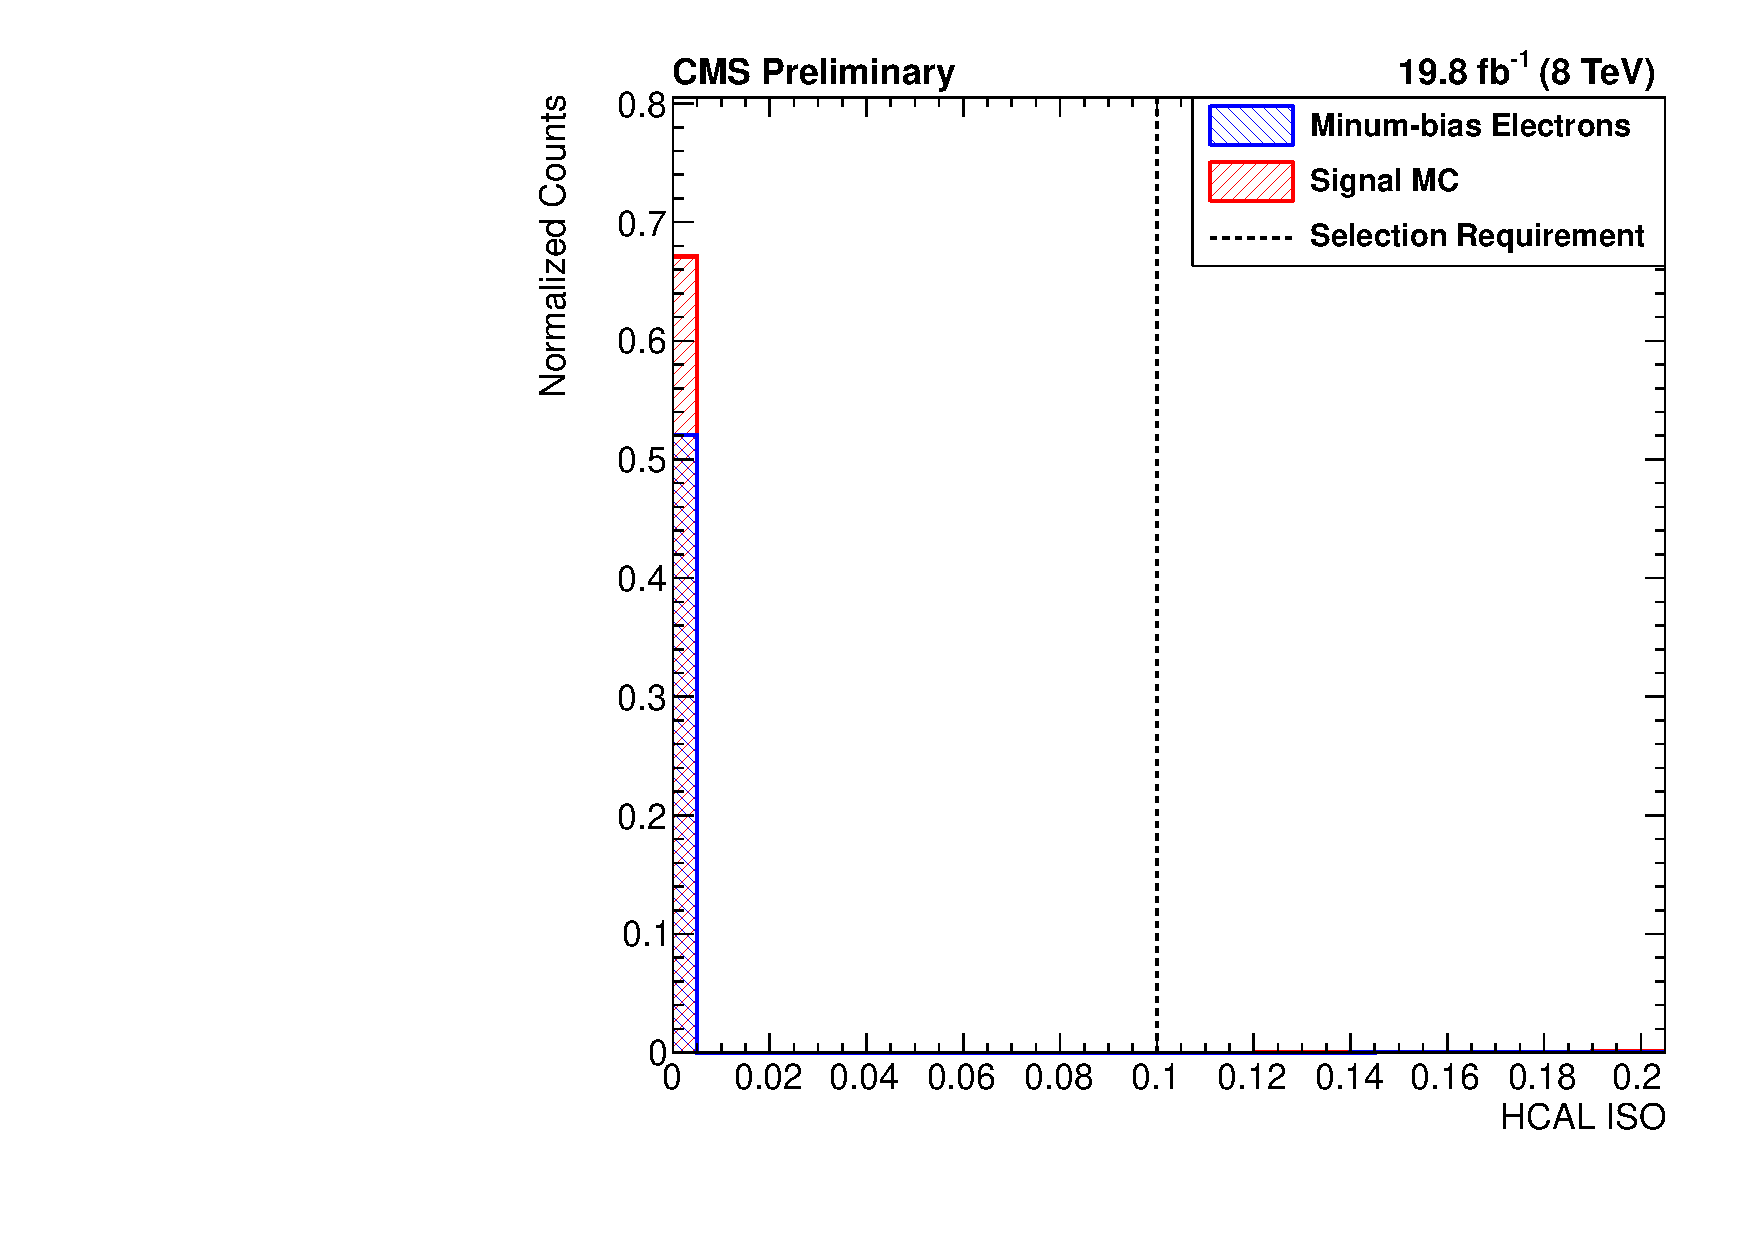
\includegraphics[width=\textwidth]{figures/e_reco_var_hcal_iso.pdf}
        \caption{}
        \label{fig:hcal_iso}
    \end{subfigure}
    \begin{subfigure}[b]{\StackedPlotWidth}
        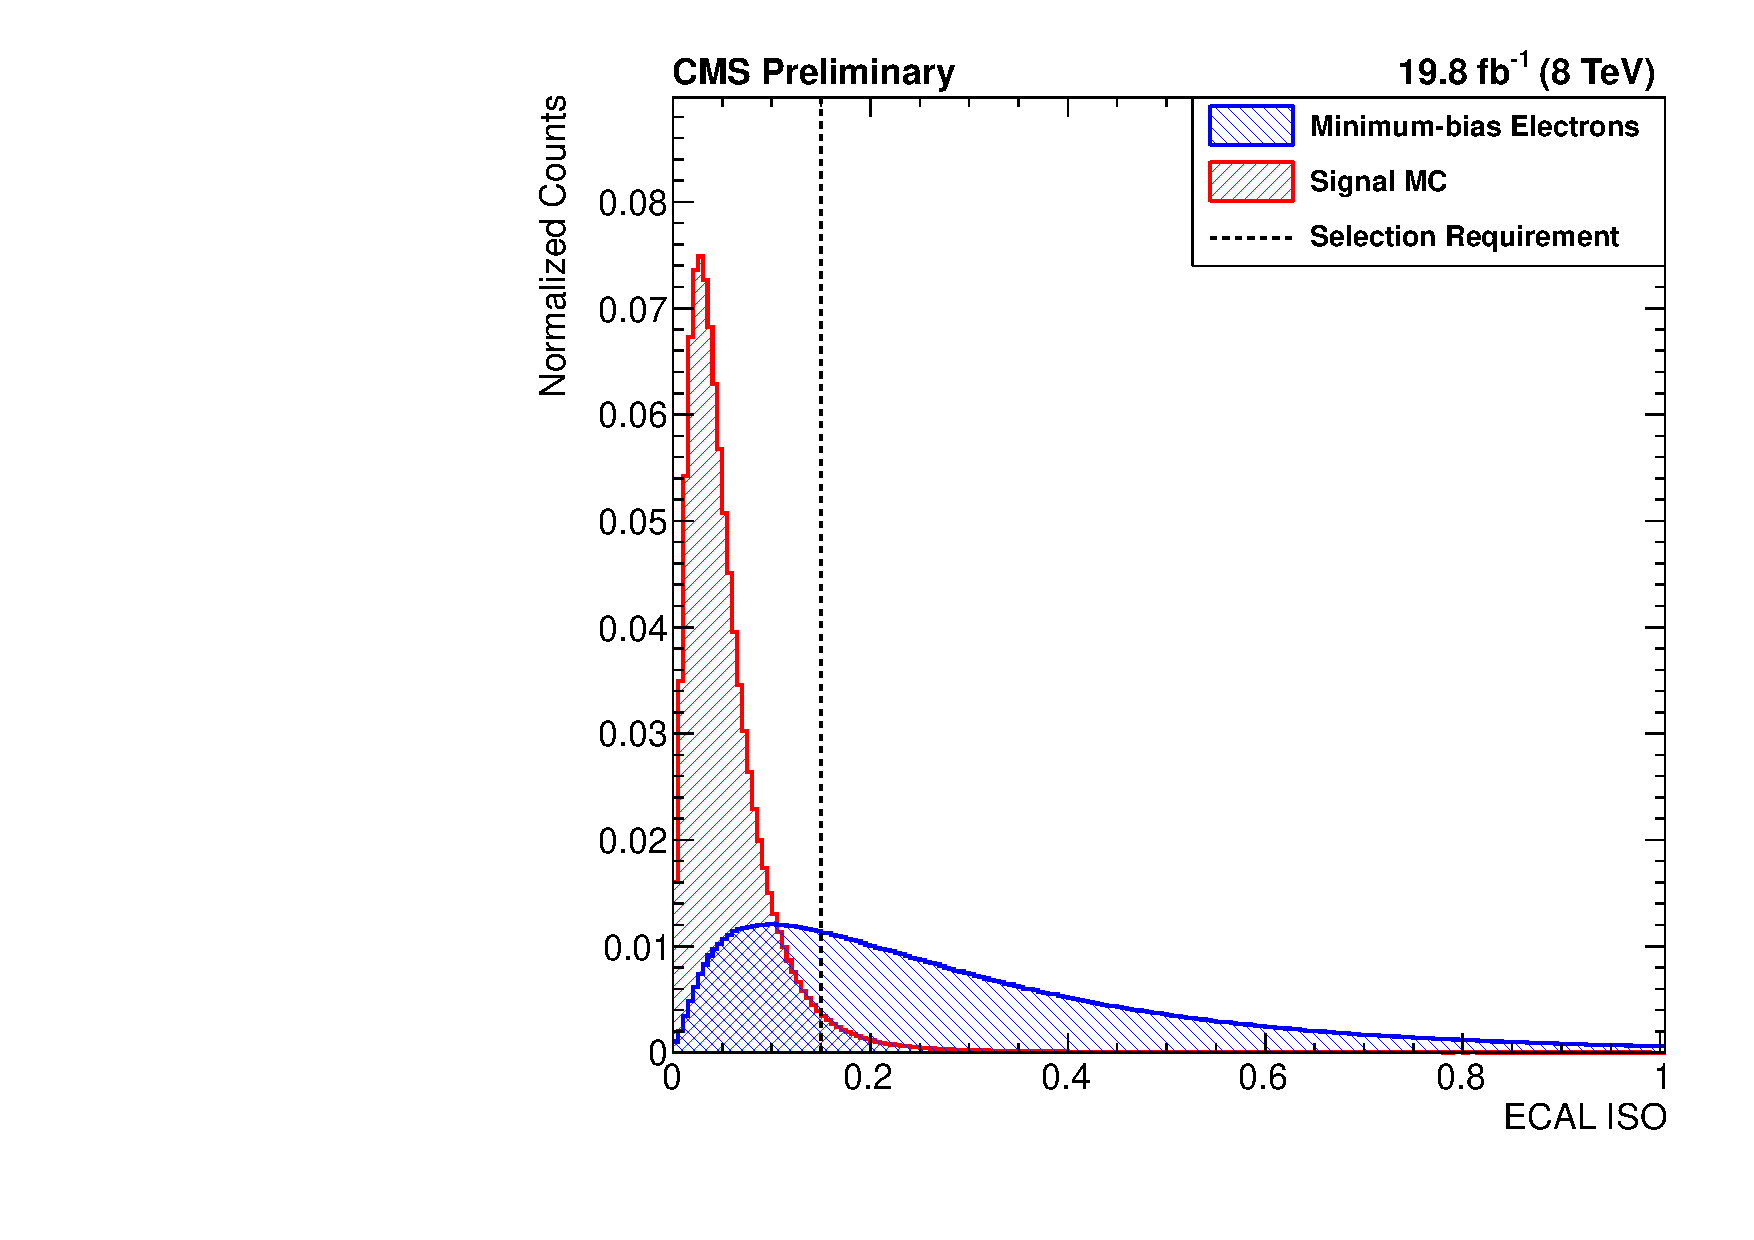
\includegraphics[width=\textwidth]{figures/e_reco_var_ecal_iso.pdf}
        \caption{}
        \label{fig:ecal_iso}
    \end{subfigure}
    \caption[
        Distributions of HCAL and ECAL isolation variables in data and MC.
    ]{
        The HCAL (top) and ECAL (bottom) isolation variable distributions for
        all electrons with $\pt > 20 \GeV$ and $|\eta| < 2.4$ in a set of
        events selected with a muon trigger and in \MADGRAPH \Ztoee MC.
    }
    \label{fig:hcal_ecal_isos}
\end{figure}

A different isolation variable is defined for selection of events in this
analysis that is more expensive to compute but takes advantage of the tracker
as well as ECAL and HCAL. This isolation uses a
``particle flow'' \cite{particle_flow_2009}\cite{particle_flow_2010} technique which
is a method of reconstructing jets that uses information for every subdetector
and tries to reconstruct the individual particles in a jet by matching them to
their responses in the various subdetectors. To keep the algorithm simple,
particle flow categorizes every particle into one of five types: photons,
electrons, muons, charged hadrons, and neutral hadrons. A photon is a particle
with energy only deposited in ECAL. An electron is a particle with an ECAL
energy deposit and a track. A muon is a track in the central tracker matched to
a track in the muon system. A charged hadron is any energy cluster in HCAL with
a possible matching ECAL cluster and track. A neutral hadron is any energy
cluster in HCAL with a possible matching ECAL cluster without a matching track.
These particle flow jets are used to calculate an energy density due to pileup,
$\rho$, in the detector which is used to remove the pileup contribution from
the isolation sum. The particle flow isolation, $\PFISO$, is given by:

\begin{equation}
    \PFISO = \DeltaRSum \frac{\left(\ptTrack + \EECAL + \EHCAL\right) - \ptElectron
    - \ESC - 0.3^{2} \pi \rho}{\ptElectron}
\end{equation}

\noindent where the variables are the same as above, with the addition of \ptTrack, which
is the \pt of all tracks in the tracker, \ptElectron, which is the \pt of the
electron's track, and $\left(0.3^{2} \pi \rho\right)$, which is the energy
around the electron due to pileup calculated from particle flow. The
particle flow isolation is normalized by the \pt of the electron. A comparison
of the \PFISO distributions between all electrons and for signal electrons is
shown in \FIG~\ref{fig:pf_iso}.

\begin{figure}[!htbp]
    \centering
    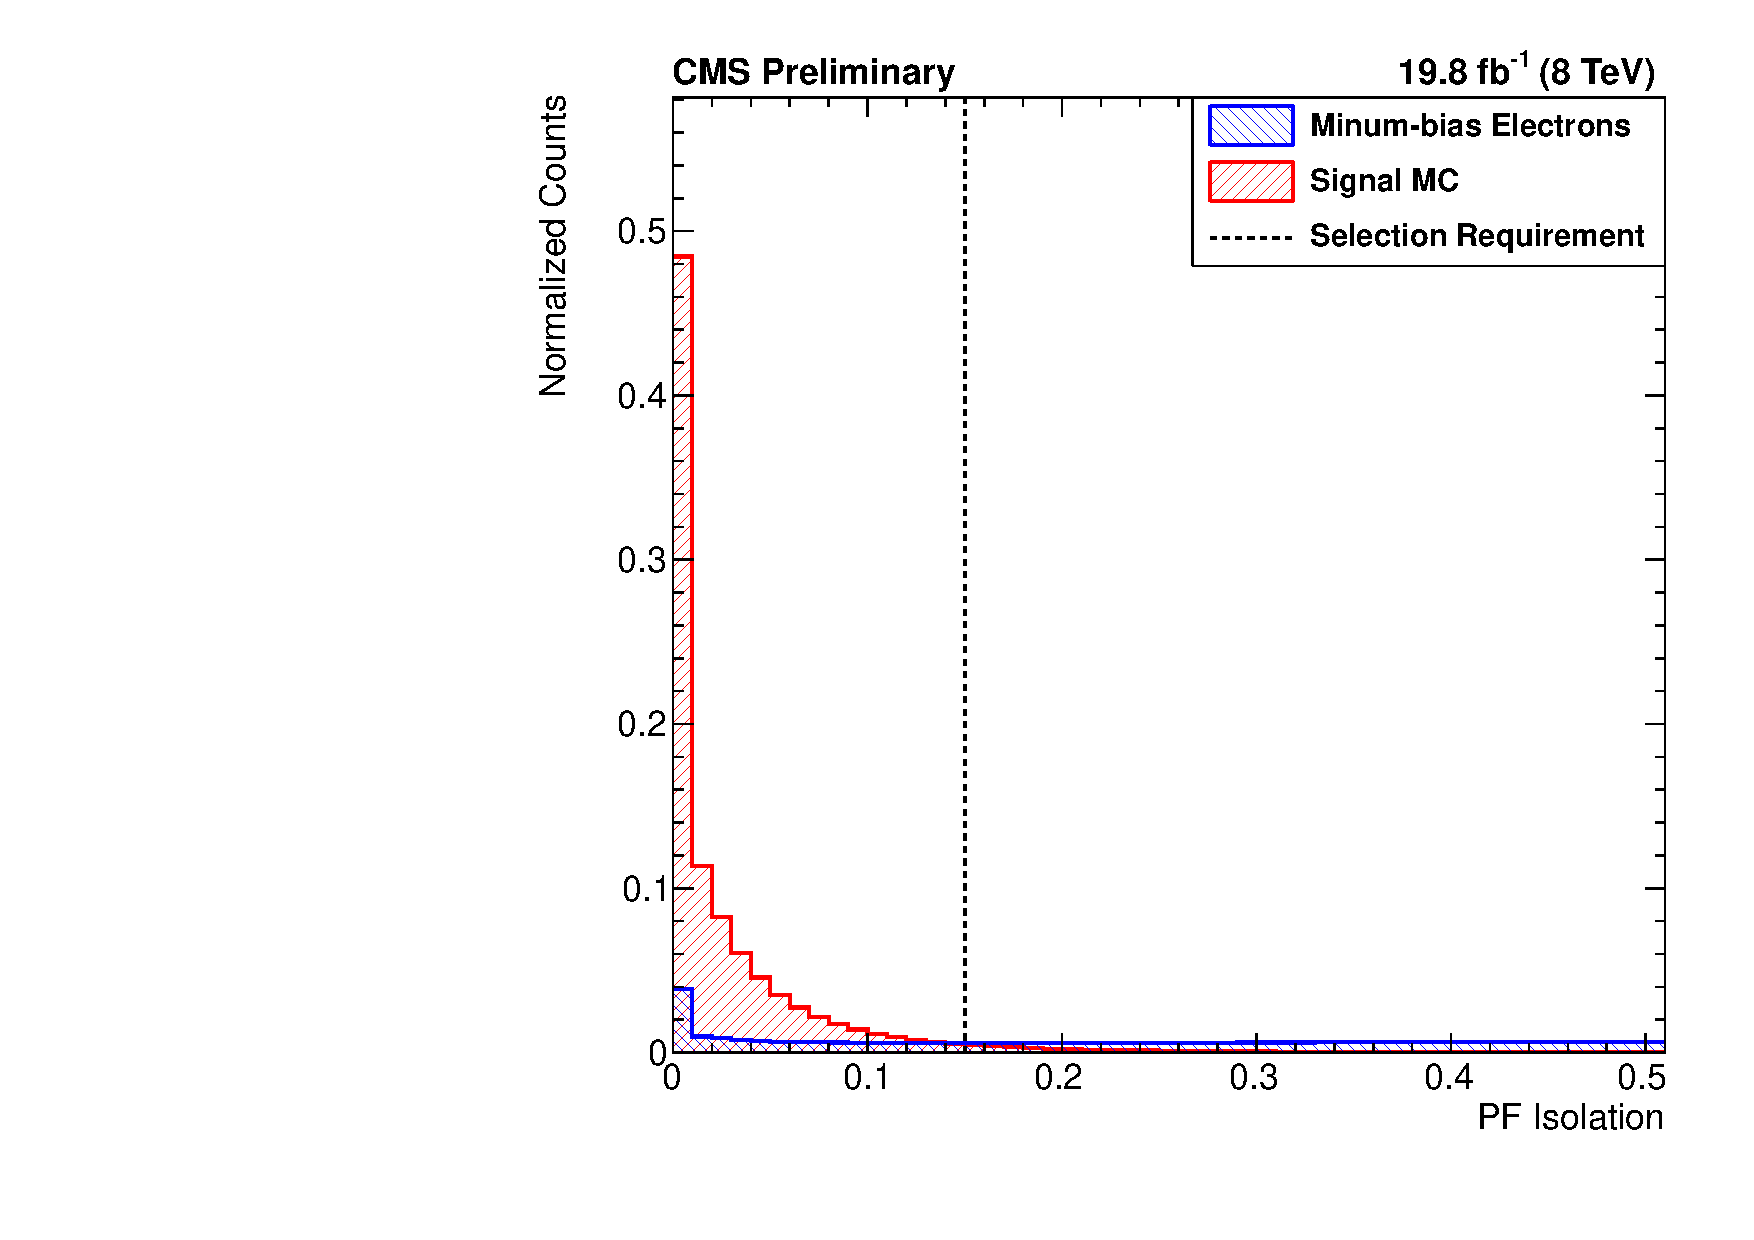
\includegraphics[width=\StackedPlotWidth]{figures/e_reco_var_iso.pdf}
    \caption[
        Distributions of particle flow isolation variables in data and MC.
    ]{
        The particle flow isolation variable distribution for all electrons
        with $\pt > 20 \GeV$ and $|\eta| < 2.4$ in a set of events selected
        with a muon trigger and in \MADGRAPH \Ztoee MC.
    }
    \label{fig:pf_iso}
\end{figure}


% The data and simulation we use
\chapter{Data and Simulation Samples}
\label{chatper:data_and_mc_samples}

\section{Data}

The data used in this analysis were collected by the CMS detector in 2012 at a
center of mass energy of \rootseight. The LHC delivered 23 \fbinv of integrated
luminosity during the year as seen in \FIG~\ref{fig:2012_luminosity}. This
period was divided into four run eras called 2012A, B, C, and D. During an era,
the LHC run parameters are kept roughly static to allow for consistent data
taking conditions. In between eras maintenance and minor upgrades are
performed on the LHC in order to deliver higher luminosity.

\begin{figure}[!htbp]
    \centering
    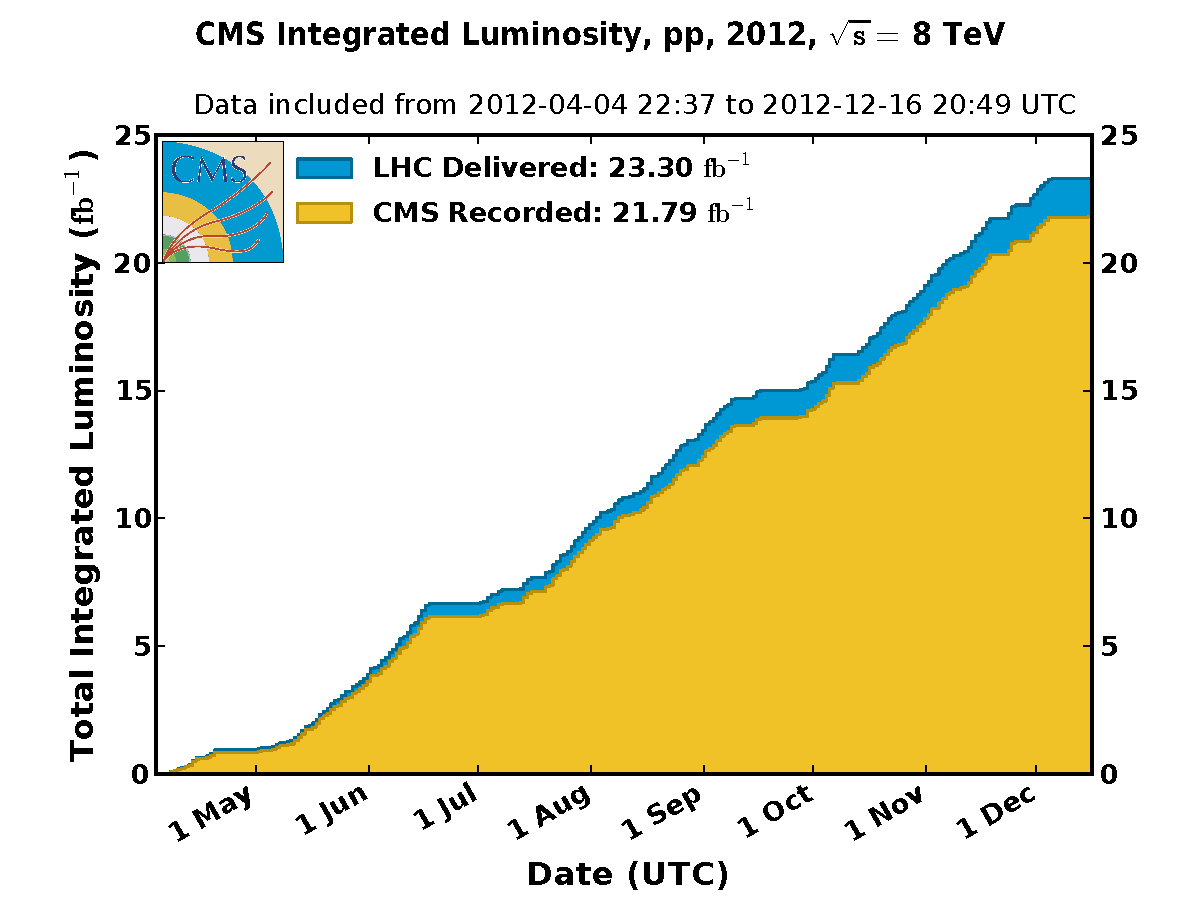
\includegraphics[width=\textwidth]{figures/2012_lumi.pdf}
    \caption[
        The integrate luminosity delivered and recorded by CMS in 2012
    ]{
        The integrate luminosity delivered and recorded by CMS in 2012. The
        flat periods in May, July, and September correspond to the boundaries
        between the run eras.
    }
    \label{fig:2012_luminosity}
\end{figure}

The data collected by CMS are split into smaller datasets based on the physics
objects contained within the events. This allows analyses to use only one or
two datasets, instead of requiring them to deal with the entirety of the CMS
data (which is many petabytes, and hence too large for most institutes to store
locally). The HLT sorts events into the various datasets based on the triggers
that the event fired. In this manner, an event can end up in multiple datasets
if it fired multiple triggers. This analysis uses the \SingleElectron dataset
which was collected with the HLT trigger \SingleElectronTrigger. These datasets
were reconstructed---converted from raw detector response into physics
objects---in January, 2013, in order to make use of the most recent
calibrations derived from the entire 2012 run. A summary of the datasets used
is provided in \TAB~\ref{table:datasets}.

\begin{table}[h]
\centering
\spacerows{1.2}
\begin{center}
    \begin{tabular}{@{}l l r@{}}
    \toprule
    Dataset Name                          & Run Dates                & Luminosity       \\
    \midrule
    /SingleElectron/Run2012A-22Jan2013-v1 & 2012-04-05 to 2012-05-08 & $889.362 \pbinv$ \\
    /SingleElectron/Run2012B-22Jan2013-v1 & 2012-05-10 to 2012-06-18 & $4.429 \fbinv$   \\
    /SingleElectron/Run2012C-22Jan2013-v1 & 2012-07-01 to 2012-09-27 & $7.152 \fbinv$   \\
    /SingleElectron/Run2012D-22Jan2013-v1 & 2012-09-28 to 2012-12-06 & $7.318 \fbinv$   \\
    \bottomrule
    \end{tabular}
\end{center}
\caption[
    Summary of datasets.
]{
    The name, run dates, and integrated luminosity of the datasets used in this
    analysis
}
\label{table:datasets}
\end{table}

Although there is a \DoubleElectron dataset which uses a trigger designed to
find Z bosons, this analysis uses the \SingleElectron dataset selected with the
\SingleElectronTrigger trigger. The primary motivation behind using this
trigger was to allow a direct comparison with a similar \phistar analysis being
performed by CMS which used \Ztomumu events selected with a single muon
trigger. The single electron trigger requires an electron with $\pt > 27$ which
passes Working Point 80 (\WPEighty). \WPEighty is a set of selection
requirements on lepton isolation and shower shape variables designed to be 80\%
efficient in selecting real electrons. The requirements that make up \WPEighty
are listed in \TAB~\ref{table:wp80}. This trigger had the lowest \pt threshold
of any single electron trigger that was unprescaled run during 2012. To
prescale a trigger means to apply a rate reduction by randomly throwing out a
certain fraction of events in order to keep the total trigger rate manageable;
as this trigger was unprescaled, no events were discarded in this manner.

\begin{table}[h]
\centering
\spacerows{1.2}
\begin{center}
    \begin{tabular}{@{}l r r@{}}
        \toprule
        Value                      & EB     & EE     \\
        \midrule
        $|\eta| <$                 & 1.4791 & 2.65   \\
        $\pt >$                    & 27     & 27     \\
        $\sigmaietaieta <$         & 0.1    & 0.03   \\
        $\ECALISO / \et <$         & 0.15   & 0.1    \\
        $\HOverE <$                & 0.1    & 0.05   \\
        $\HCALISO / \et <$         & 0.1    & 0.1    \\
        Pixel Matching $\ge$       & 1      & 1      \\
        $|\ooeoop| <$              & 0.05   & 0.05   \\
        $|\Delta \eta| <$          & 0.007  & 0.007  \\
        $|\Delta \phi| <$          & 0.06   & 0.03   \\
        \bottomrule
    \end{tabular}
\end{center}
\caption[
    The selection requirements for the \SingleElectronTrigger trigger.
]{
    The selection requirements for the \SingleElectronTrigger trigger for
    electrons which end up in the barrel region or the endcap region of ECAL.
    The variables used are detailed in \SEC~\ref{sec:electron_variables}.
}
\label{table:wp80}
\end{table}

The events from the \SingleElectron sample are further filtered for quality. A
centrally produced list of good luminosity segments is used to select only
events in which no part of the detector was malfunctioning or disabled. After
accounting for detector dead time and beam quality, \GoodLumiNumber of
integrated luminosity are used for physics analysis.

\section{Monte Carlo Datasets}
\label{ssec:monte_carlo}

This analysis makes use of numerous simulated data samples---colloquially
referred to as Monte Carlo (MC)---in order to estimate backgrounds and signal
yields, derive scale factors, and correct for the effects of bin migration on
the final measurement. All the MC used in this analysis were centrally
generated by the CMS collaboration. A \DYtoll signal sample and a
$\ttbar\text{+jets}$ background sample were generated with \MADGRAPH
\cite{alwall2014}. Diboson ($\Z\Z$, $\W\Z$, $\W\W$) background samples were
generated with \PYTHIA \cite{sjostran2006}. Background samples consisting of
$\tbar \W$, $t \W$, and $\DYtotautau$ were generated using \POWHEG
\cite{nason2004}\cite{alioli2010}\cite{re2011}. A secondary signal MC was also
generated with \POWHEG. The details of these samples are listed in
\TAB~\ref{table:mc}.

\begin{table}[h]
\centering
\spacerows{1.2}
\begin{center}
    \begin{tabular}{@{}l l l r r@{}}
    \toprule
    Process                                & Requirements     & Generator  & $\sigma$ (pb) & Events $(\times 10^{6})$ \\
    \midrule
    \DYtoll                                & $\mll > 50 \GeV$ &  \MADGRAPH & 3531.9 (NNLO) & 30.460 \\
    \DYtoee                                & $\mll > 20 \GeV$ &  \POWHEG   & 1966.7        & 3.297\\
    \DYtotautau                            & $\mll > 20 \GeV$ &  \POWHEG   & 1966.7        & 3.297  \\
    \ttbar                                 &                  &  \MADGRAPH & 23.64         & 3.984  \\
    $t \rightarrow \W+b \rightarrow X$     &                  &  \POWHEG   & 11.1          & 0.498  \\
    $\tbar \rightarrow \W+b \rightarrow X$ &                  &  \POWHEG   & 11.1          & 0.493  \\
    $\W\W$                                 &                  &  \PYTHIA   & 54.84         & 10.000 \\
    $\W\Z$                                 &                  &  \PYTHIA   & 33.21         & 10.000 \\
    $\Z\Z$                                 &                  &  \PYTHIA   & 17.7          & 9.800  \\
    \bottomrule
    \end{tabular}
\end{center}
\caption[
    Summary of MC samples.
]{
    Summary of the MC samples used in this analysis. The Drell-Yan MC samples
    have mass requirements on the events while the other MC samples have none.
    All cross sections are NLO unless otherwise stated.
}
\label{table:mc}
\end{table}

After the generation step, MC is sent through a full detector simulation which
uses \GEANTfour \cite{agostinelli2003} to mimic the detector response. This
detector response is reconstructed using the full CMS reconstruction chain to
produce MC files in a format identical to actual data.

\TODO{Jeremy says MC is overlaid with minibias MC. As many as 200 events are
used at a time.}

MC events have actual data events overlaid on top of them to better match the
conditions found in actual running. These overlaid events come from the minimum
bias dataset, which is selected with a minimum of requirements imposed on the
event in order to select events that are ``typical'' of proton-proton
collisions. Additional events are overlaid in order to simulate pileup. The
number of pileup events overlaid is drawn from a distribution that is expected
to match the distribution seen in data. \TODO{Jeremy says about the next part:
"Oh really?"} Of course, it is not possible to
perfectly predict the data distribution and so a reweighting technique is used
to match the MC distribution to the data. The distribution in MC is compared to
that in data and the ratio of these distributions is assigned as a weight to
each MC event to force the distributions to match.

\section{Scale Factors}
\label{sec:scale_factors}

The detector response to various signals is not always perfectly simulated in
MC and so the efficiencies of various selection requirements are not the same
in data and MC. In order to correct for this difference, each event in MC is
reweighed with a series of scale factors which are the efficiency of some
selection requirement in data divided by the same efficiency as measured on MC,
as follows:

\begin{equation}
    \label{eq:sf}
    \text{SF} = \frac{\effdata}{\effmc}
\end{equation}

Three scale factors are applied to each event: trigger, reconstruction, and
identification. The trigger scale factors were measured by us and are detailed
in \SEC~\ref{ssec:sf_trigger} while the reconstruction and identification scale
factors were measured centrally by the CMS collaboration. The centrally
produced values are used as doing so is a requirement of passing the internal
analysis review. The methods used to measure the reconstruction and isolation
scale factors are summarized in \SECS~\ref{ssec:sf_reconstruction} and
\ref{ssec:sf_id} because the papers detailing them are not public

\subsection{Tag and Probe}

Tag and Probe (\TnP) is a minimally-biased method of calculating the efficiency
of some analysis selection requirement. \TnP takes advantage of the well-known
mass and narrow width of the \Z boson to select a set of electrons for which
very few selection requirements have been applied. This is done by finding one
high-quality electron, the tag, and another minimally-biased object, the probe,
that could be an electron, such as a supercluster. The invariant mass of these
objects is computed and if it is near the \Z mass peak, it is very likely that
the probe is also an electron.

Once a set of minimally-biased probe electrons is constructed, the selection
requirement can be applied to them. The efficiency of that requirement is then
the number of probes that passs divided by the total number in the sample as
follows:

\begin{equation}
    \label{eq:eff}
    \eff = \frac{\nobs_{\pass}}{\nobs_{\total}}
\end{equation}

\subsection{Single Electron Trigger}
\label{ssec:sf_trigger}

The efficiency of the HLT trigger used in this analysis,
\SingleElectronTrigger, is measured using \TnP on the primary dataset. The
efficiency is measured in bins of probe \pt and probe $\eta$ with bin
boundaries of \{30, 40, 50, 70, 250\} in \pt and \{-2.1, -2.0, -1.556, -1.442,
-0.8, 0., 0.8, 1.442, 1.556, 2.0, 2.1\} in $\eta$.

Both the tag electron and the probe electron are required to satisfy $|\eta| <
2.1$, $\pt > 30$, and to pass \EGTIGHT requirements. These requirements are the
same as required of the \CentralElectron in the full analysis selection, and
hence the efficiency is measured relative to that selection. The pair must have
an invariant mass such that \MassRange. The tag electron is required to be
matched to an electron that fired the trigger with $\Delta R < 0.3$. There is
no requirement placed on the charge of the electron pair. Events with three or
more electrons that pass these requirements are rejected.

Probes are considered passing if they are also matched to an electron that
fired the trigger with $\Delta R < 0.3$, and failing otherwise. The efficiency
in each bin is the number of passing probes divided by the number of failing
probes, where the number of passing and failing probes is determined by using a
simple count. In an individual event, both electrons are tried as a tag so that
an event may contribute to the efficiency measurement twice if both electrons
pass the tag requirements.

The efficiency is computed in exactly the same way on the \MADGRAPH sample. The
MC events are reweighted for pileup, reconstruction efficiency, and
identification efficiency before the trigger efficiency is measured. The
measured efficiencies for data and MC are listed in
\TABS~\ref{trigger_eff_data} and \ref{trigger_eff_mc}, respectively.

In the case of the trigger, because either electron could cause the event to
pass, the scale factors can not be computed for each bin, but instead must be computed
for each pair of bins. If only one electron in the event has $\pt > 30$ and
$|\eta| < 2.1$ than the scale factor is simply that given by \EQ~\ref{eq:sf}, but if both
electrons pass the requirements than either could have fired the trigger and so
the scale factor is given by:

\begin{equation} \label{eq:sf_double}
    \text{SF}_{1 \text{ or } 2}
    =
    \frac{
        1 - \left( 1 - \effdata_{0} \right) \left( 1 - \effdata_{1} \right)
    } {
        1 - \left( 1 - \effmc_{0} \right) \left( 1 - \effmc_{1} \right)
    }
\end{equation}

Where $\effdata_{0,1}$ is the efficiency as measured in data for the 0th and
1st electrons, and $\effmc_{0,1}$ is the efficiency as measured in MC.
\EQ~\ref{eq:sf_double} is just the probability that one or both of the
electrons fired the trigger divided by the same quantity in MC. This equation
assumes that the probability of one electron firing the trigger is uncorrelated
with the probability of the other electron firing the trigger.

% Data
\begin{table}[h]
\centering
\spacerows{1.5}
\begin{center}
    \begin{tabular}{@{}c c c c c c@{}}
    \toprule
    $\eta$ & 30---40 \GeV & 40---50 \GeV & 50---70 \GeV & 70---250 \GeV  \\
    \midrule
    \numrange{-2.1}{-2} & $0.741^{+0.003}_{-0.003}$ & $0.773^{+0.003}_{-0.003}$ & $0.780^{+0.005}_{-0.005}$ & $0.79^{+0.01}_{-0.01}$  \\
    \numrange{-2}{-1.556} & $0.734^{+0.001}_{-0.001}$ & $0.772^{+0.001}_{-0.001}$ & $0.786^{+0.002}_{-0.002}$ & $0.792^{+0.005}_{-0.005}$  \\
    \numrange{-1.556}{-1.442} & $0.725^{+0.003}_{-0.003}$ & $0.821^{+0.002}_{-0.002}$ & $0.809^{+0.004}_{-0.004}$ & $0.848^{+0.010}_{-0.010}$  \\
    \numrange{-1.442}{-0.8} & $0.8930^{+0.0005}_{-0.0005}$ & $0.9396^{+0.0003}_{-0.0004}$ & $0.9509^{+0.0006}_{-0.0006}$ & $0.966^{+0.001}_{-0.001}$  \\
    \numrange{-0.8}{0} & $0.9213^{+0.0004}_{-0.0004}$ & $0.9528^{+0.0002}_{-0.0002}$ & $0.9601^{+0.0004}_{-0.0004}$ & $0.9692^{+0.0010}_{-0.0010}$  \\
    \numrange{0}{0.8} & $0.9174^{+0.0004}_{-0.0004}$ & $0.9473^{+0.0003}_{-0.0003}$ & $0.9561^{+0.0004}_{-0.0004}$ & $0.963^{+0.001}_{-0.001}$  \\
    \numrange{0.8}{1.442} & $0.8964^{+0.0005}_{-0.0005}$ & $0.9424^{+0.0003}_{-0.0003}$ & $0.9533^{+0.0006}_{-0.0006}$ & $0.966^{+0.001}_{-0.001}$  \\
    \numrange{1.442}{1.556} & $0.714^{+0.003}_{-0.003}$ & $0.823^{+0.002}_{-0.002}$ & $0.827^{+0.004}_{-0.004}$ & $0.861^{+0.009}_{-0.010}$  \\
    \numrange{1.556}{2} & $0.758^{+0.001}_{-0.001}$ & $0.800^{+0.001}_{-0.001}$ & $0.811^{+0.002}_{-0.002}$ & $0.823^{+0.005}_{-0.005}$  \\
    \numrange{2}{2.1} & $0.764^{+0.003}_{-0.003}$ & $0.792^{+0.002}_{-0.002}$ & $0.797^{+0.005}_{-0.005}$ & $0.82^{+0.01}_{-0.01}$  \\
    \bottomrule
    \end{tabular}
\end{center}
\caption{
    The electron trigger efficiency in data.
}
\label{trigger_eff_data}
\end{table}

% MC
\begin{table}[h]
\centering
\spacerows{1.5}
\begin{center}
    \begin{tabular}{@{}c c c c c c@{}}
    \toprule
    $\eta$ & 30---40 \GeV & 40---50 \GeV & 50---70 \GeV & 70---250 \GeV  \\
    \midrule
    \numrange{-2.1}{-2} & $0.734^{+0.004}_{-0.004}$ & $0.769^{+0.004}_{-0.004}$ & $0.771^{+0.008}_{-0.008}$ & $0.76^{+0.02}_{-0.02}$  \\
    \numrange{-2}{-1.556} & $0.736^{+0.002}_{-0.002}$ & $0.768^{+0.002}_{-0.002}$ & $0.779^{+0.003}_{-0.003}$ & $0.789^{+0.008}_{-0.008}$  \\
    \numrange{-1.556}{-1.442} & $0.791^{+0.004}_{-0.004}$ & $0.847^{+0.003}_{-0.003}$ & $0.850^{+0.006}_{-0.006}$ & $0.87^{+0.01}_{-0.02}$  \\
    \numrange{-1.442}{-0.8} & $0.9395^{+0.0006}_{-0.0006}$ & $0.9612^{+0.0004}_{-0.0004}$ & $0.9690^{+0.0007}_{-0.0008}$ & $0.980^{+0.002}_{-0.002}$  \\
    \numrange{-0.8}{0} & $0.9469^{+0.0005}_{-0.0005}$ & $0.9670^{+0.0003}_{-0.0003}$ & $0.9745^{+0.0005}_{-0.0005}$ & $0.982^{+0.001}_{-0.001}$  \\
    \numrange{0}{0.8} & $0.9466^{+0.0005}_{-0.0005}$ & $0.9665^{+0.0003}_{-0.0003}$ & $0.9739^{+0.0005}_{-0.0006}$ & $0.982^{+0.001}_{-0.001}$  \\
    \numrange{0.8}{1.442} & $0.9364^{+0.0007}_{-0.0007}$ & $0.9597^{+0.0004}_{-0.0004}$ & $0.9668^{+0.0008}_{-0.0008}$ & $0.979^{+0.002}_{-0.002}$  \\
    \numrange{1.442}{1.556} & $0.779^{+0.004}_{-0.005}$ & $0.841^{+0.003}_{-0.003}$ & $0.842^{+0.006}_{-0.006}$ & $0.86^{+0.02}_{-0.02}$  \\
    \numrange{1.556}{2} & $0.749^{+0.002}_{-0.002}$ & $0.786^{+0.002}_{-0.002}$ & $0.798^{+0.003}_{-0.003}$ & $0.810^{+0.008}_{-0.008}$  \\
    \numrange{2}{2.1} & $0.737^{+0.004}_{-0.004}$ & $0.769^{+0.004}_{-0.004}$ & $0.779^{+0.007}_{-0.008}$ & $0.82^{+0.02}_{-0.02}$  \\
    \bottomrule
    \end{tabular}
\end{center}
\caption{
    The electron trigger efficiency in \MADGRAPH MC.
}
\label{trigger_eff_mc}
\end{table}

\subsection{Electron Reconstruction}
\label{ssec:sf_reconstruction}

Electron reconstruction begins with the assembly of a supercluster in ECAL and
ends with the matching of a supercluster to a track in the tracker. The details
of Electron reconstruction are described in
\SEC~\ref{sec:electron_reconstruction}. The efficiency of an electron with $\pt
> 20 \GeV$ depositing enough energy in ECAL to be reconstructed into a
supercluster is very high, although the exact efficiency must be measured in
MC as there is no more basic object with which to perform \TnP to measure it in
data. Scale factors for matching a track given that a supercluster has already
been found were measured centrally by the CMS collaboration using \TnP
\cite{gsf_scale_factors_2013}. A summary of their method follows.

The events used to measure the reconstruction scale factors are selected with the
dedicated electron \TnP Trigger: \TnPTrigger. This trigger requires one
electron with $\pt > 20 \GeV$ which must also pass very tight isolation and ID
requirements while requiring only a low energy ($\et > 4 \GeV$) supercluster as
the other leg. The trigger rate is kept down by requiring that the invariant
mass of these two objects is greater than $50 \GeV$.

The events selected by the trigger are further required to pass a set of
selection requirements. The tag electron is required to pass \EGTIGHT, have
$\pt > 25 \GeV$, and $|\eta| < 2.5$. Electrons are rejected if they fall in the
seem between EB and EE ($1.4442 < |\eta| < 1.566$). The tag must also be
matched to the tight leg of the \TnP trigger. The probe supercluster has
minimal requirements applied; it is required to have tracker isolation $<
0.15$. For the MC sample, the tag is only required to be matched to a generator
level electron with $\Delta R < 0.2$. Additionally, the event is required to
have low \particleflow missing energy $\PFMET < 20 \GeV$.

The events were binned in terms of probe's $\pt$ and $\eta$ as well as whether
the probe passed or failed. In each bin, the \mee distribution was constructed
and a template consisting of the sum of a Gaussian smeared \Ztoee MC sample and
an exponential background was fitted. The number of events predicted by the
signal fit on the passing sample, failing sample, and sum of the two samples
was used to get the efficiency. A similar process was performed on MC, although
instead of a fit a simple counting of passing events was performed (as there is
no background in MC). The resulting scale factors are given in
\TAB~\ref{table:gsf_scale_factor}.

\begin{table}[h]
\centering
\spacerows{1.5}
\begin{center}
    \begin{tabular}{@{}c c c c c@{}}
    \toprule
    $|\eta|$                 & 20--30 \GeV                        & 30--40 \GeV                        & 40--50 \GeV                        & $>$ 50 \GeV                        \\
    \midrule
    \numrange{0.0}{0.8}      & $\effstatsys{0.982}{0.003}{0.012}$ & $\effstatsys{0.988}{0.001}{0.008}$ & $\effstatsys{0.990}{0.001}{0.004}$ & $\effstatsys{0.990}{0.001}{0.004}$ \\
    \numrange{0.8}{1.4442}   & $\effstatsys{0.993}{0.002}{0.012}$ & $\effstatsys{0.993}{0.001}{0.008}$ & $\effstatsys{0.993}{0.001}{0.004}$ & $\effstatsys{0.991}{0.001}{0.004}$ \\
    \numrange{1.4442}{1.566} & $\effstatsys{1.016}{0.012}{0.020}$ & $\effstatsys{0.985}{0.004}{0.009}$ & $\effstatsys{0.987}{0.004}{0.004}$ & $\effstatsys{0.974}{0.009}{0.006}$ \\
    \numrange{1.566}{2.0}    & $\effstatsys{0.988}{0.003}{0.012}$ & $\effstatsys{0.993}{0.002}{0.008}$ & $\effstatsys{0.992}{0.001}{0.004}$ & $\effstatsys{0.990}{0.003}{0.004}$ \\
    \numrange{2.0}{2.5}      & $\effstatsys{1.002}{0.004}{0.012}$ & $\effstatsys{1.004}{0.002}{0.008}$ & $\effstatsys{1.005}{0.002}{0.004}$ & $\effstatsys{0.998}{0.004}{0.004}$ \\
    \bottomrule
    \end{tabular}
\end{center}
\caption[
    Scale factors for GSF electron reconstruction.
]{
    Scale factors for GSF electron reconstruction. The upper uncertainty listed
    is statistical, the lower is systematic.
}
\label{table:gsf_scale_factor}
\end{table}

\subsection{Electron Identification}
\label{ssec:sf_id}

Not all electrons which are reconstructed pass the ID criteria used in this
analysis, specifically \EGMEDIUM and \EGTIGHT, the details of which are covered
in \SEC~\ref{ssec:electron_selection}. The efficiency of going from a
reconstructed electron to one which passes the identification criteria is
measured centrally by the CMS collaboration using \TnP \cite{cms_an_2014-055}.
A summary of their method follows.

The events used for this measurement were selected using two triggers: \\
\TnPTrigger, which is described above, and \TnPTriggerSecond, which requires
one electron with $\pt > 17 \GeV$ and tight isolation and ID requirements while
also requiring a reconstructed second electron (as opposed to a supercluster as
required by the first trigger) with $\pt > 8 \GeV$. It further requires a
dielectron invariant mass of $\mee > 50 \GeV$.

The tag electrons are required to pass \EGTIGHT, have $\pt > 25 \GeV$, and
$|\eta| < 2.5$; they are rejected if they fall in the seem between EB and EE
($1.4442 < |\eta| < 1.566$). The tag is not required to match the trigger.
Probe electrons have the same $\eta$ requirements as tags, but are only
required to have $\pt > 10 \GeV$. Passing probes pass the ID criteria under
investigation, failing probes fail the ID criteria. The invariant mass of the
tag and probe pair is required to be near the \Z mass peak (\MassRange). The
electrons are required to have charges of opposite sign. In MC, the probe is
only required to be matched to a generator electron with $\Delta R < 0.2$.

The efficiencies are then calculated by fitting the \mee distributions using a
template constructed with a \Ztoee MC sample and an exponential background. The
three categories (passing probes, failing probes, and all probes) are then
simultaneously fit with this template and the number of fitted signal events is
used to derive an efficiency. A simple count of events is used for the MC
efficiency instead of a fit. The resulting scale factors are given in
\TABS~\ref{table:tight_scale_factor} and \ref{table:medium_scale_factor}.

\begin{table}[h]
\centering
\spacerows{1.5}
\begin{center}
    \begin{tabular}{@{}c c c c c@{}}
    \toprule
    $|\eta|$                 & 20--30 \GeV               & 30--40 \GeV               & 40--50 \GeV               & 50--200 \GeV \\
    \midrule
    \numrange{0.0}{0.8}      & $0.960_{-0.003}^{+0.003}$ & $0.978_{-0.001}^{+0.001}$ & $0.981_{-0.001}^{+0.001}$ & $0.982_{-0.002}^{+0.002}$ \\
    \numrange{0.8}{1.4442}   & $0.936_{-0.004}^{+0.004}$ & $0.958_{-0.002}^{+0.002}$ & $0.969_{-0.001}^{+0.001}$ & $0.969_{-0.002}^{+0.002}$ \\
    \numrange{1.4442}{1.566} & $0.933_{-0.017}^{+0.015}$ & $0.907_{-0.008}^{+0.008}$ & $0.904_{-0.004}^{+0.004}$ & $0.926_{-0.011}^{+0.011}$ \\
    \numrange{1.566}{2.0}    & $0.879_{-0.007}^{+0.007}$ & $0.909_{-0.003}^{+0.003}$ & $0.942_{-0.002}^{+0.002}$ & $0.957_{-0.004}^{+0.004}$ \\
    \numrange{2.0}{2.5}      & $0.974_{-0.004}^{+0.004}$ & $0.987_{-0.004}^{+0.004}$ & $0.991_{-0.003}^{+0.003}$ & $0.999_{-0.005}^{+0.005}$ \\
    \bottomrule
    \end{tabular}
\end{center}
\caption{
    Scale factors for \EGTIGHT electron ID.
}
\label{table:tight_scale_factor}
\end{table}

\begin{table}[h]
\centering
\spacerows{1.5}
\begin{center}
    \begin{tabular}{@{}c c c c c@{}}
    \toprule
    $|\eta|$                 & 20--30 \GeV               & 30--40 \GeV               & 40--50 \GeV               & 50--200 \GeV \\
    \midrule
    \numrange{0.0}{0.8}      & $0.986_{-0.001}^{+0.002}$ & $1.002_{-0.001}^{+0.001}$ & $1.005_{-0.001}^{+0.001}$ & $1.004_{-0.001}^{+0.001}$ \\
    \numrange{0.8}{1.4442}   & $0.959_{-0.003}^{+0.003}$ & $0.980_{-0.001}^{+0.001}$ & $0.988_{-0.001}^{+0.001}$ & $0.988_{-0.002}^{+0.002}$ \\
    \numrange{1.4442}{1.566} & $0.967_{-0.013}^{+0.007}$ & $0.950_{-0.007}^{+0.006}$ & $0.958_{-0.005}^{+0.005}$ & $0.966_{-0.009}^{+0.009}$ \\
    \numrange{1.566}{2.0}    & $0.941_{-0.005}^{+0.005}$ & $0.967_{-0.003}^{+0.003}$ & $0.992_{-0.002}^{+0.002}$ & $1.000_{-0.003}^{+0.003}$ \\
    \numrange{2.0}{2.5}      & $1.020_{-0.003}^{+0.003}$ & $1.021_{-0.003}^{+0.003}$ & $1.019_{-0.002}^{+0.002}$ & $1.022_{-0.004}^{+0.004}$ \\
    \bottomrule
    \end{tabular}
\end{center}
\caption{
    Scale factors for \EGMEDIUM electron ID.
}
\label{table:medium_scale_factor}
\end{table}

\section{Electron Dressing}
\label{sec:electron_dressing}

\begin{figure}[!htbp]
    \centering
    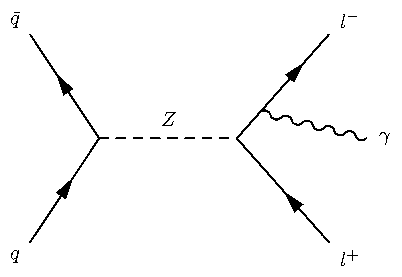
\includegraphics[width=0.65\textwidth]{figures/fsr.pdf}
    \caption{
        Feynman diagram of \Ztoll with FSR.
        % From http://www.physik.uzh.ch/~che/FeynDiag/ CC-BY-SA
    }
    \label{fig:fsr_diagram}
\end{figure}

After the \Ztoee decay, the electrons can radiate photons in a process known as
as final state radiation (FSR). The diagram of this process is shown in
\FIG~\ref{fig:fsr_diagram}. Some theoretical models will want to neglect FSR
while others will attempt to include it in order to better predict what the
experiments will measure. What is measured depends on the lepton being measured
and on the detector. In the case of electrons in CMS, what is measured is a
supercluster which includes the energy of nearby photons. Muons, on the other
hand, are minimum ionizing particles and so their momentum is measured using
the tracker and muon chambers but not ECAL, and so there is no contribution
from photons.

In order to accommodate comparison of our results to other measurements and
theoretical models, regardless of how those models treat FSR, we define three
different types of generator level electron in MC. Each of these three
definitions is then used whenever generator MC is used in the analysis in order
to produce three different final results. This is done to make it easy to
compare our results to theoretical models regardless of how the models handle
FSR. The three definitions of generator electrons are as follows:

\begin{description}
    \item[Born] A generator electron immediately after the \Ztoee decay and
        before and FSR. These electrons are what are predicted by models that
        neglect FSR.
    \item[Bare] A generator electron after it has shed all of its FSR photons.
        These electrons match how muons are measured and so are more easily
        comparable to muon results.
    \item[Dressed] A bare electron, but with its FSR photons added back in
        vector sum if they are within $\Delta R < 0.1$ of the electron. These
        electrons closely match the electrons measured at CMS.
\end{description}


% Analysis and conclusion
\chapter{Event Selection}
\label{event_selection_chapter}

This chapter details the requirements used to select events for the analysis.
It also covers the data used and the Monte Carlo (MC) used. The final state we
are considering is \Ztoee.

\section{Acceptance}

The acceptance region is a definition of what events, assuming that there are
no limitations due to the detector design, we include in our analysis. It is
essential to define an acceptance region so that our final result can be
compared to other measurements and to theory without forcing other groups to
attempt to correct for our experimental effects. The acceptance region defines
what sort of physics results we can make statements about, and also determines
the value of the effective cross-section of the \Z.

Our acceptance is defined by the kinematics of the two electrons and the mass
of the Z boson. One of the electrons, called the \CentralElectron, is required
to have $\pt > 30 \GeV$ and to be within the central region of the detector
(hence the name) with $|\eta| < 2.1$. The other electron, called the
\ExtendedElectron, has looser requirements; it must have $\pt > 20 \GeV$ and is
not required to be as central with $|\eta| < 2.4$. The requirements on the
\CentralElectron were selected in conjunction with the \Ztomumu measurement of
\phistar at CMS so that that measurement and this one could be easily combined
into a joint measurement. The pseudorapidity limit was selected to match the
most efficient region of CMS's single muon trigger, while the transverse
momentum threshold was dictated by threshold on single electron trigger. The
pseudorapidity limit on the \ExtendedElectron was chosen to keep all of the
electrons within the region covered by the tracker (which allows a better
angular measurement than ECAL alone), while the transverse momentum threshold
was selected because for $\pt < 20 \GeV$ the rate of fake electrons increases.

\begin{figure}[tb]
    \centering
    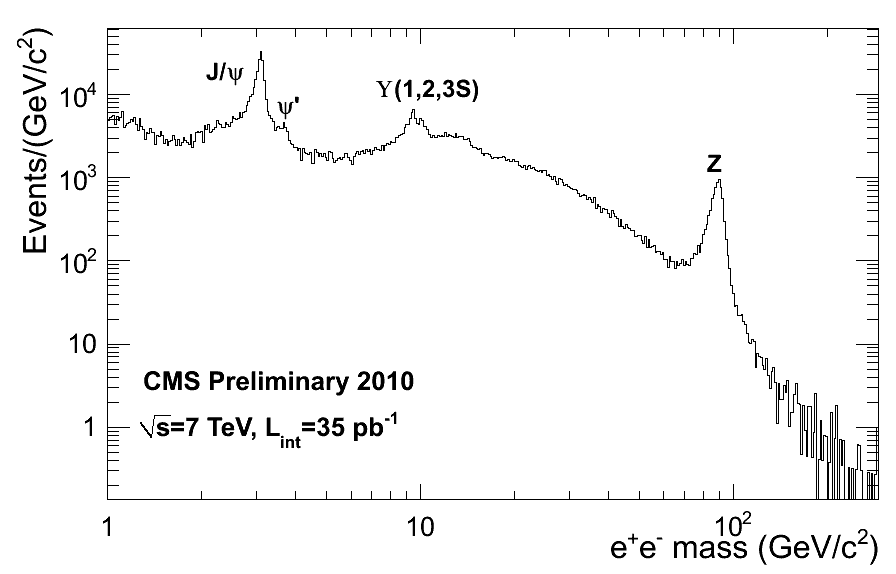
\includegraphics[width=\textwidth]{figures/dielectron_mass_7tev.png}
    \caption{The spectrum of \ee events as measured by CMS in 2010.}
    \label{fig:ee_spectrum}
\end{figure}

There are other particles, like the \jpsi, that decay to \ee pairs as shown in
\FIG~\ref{fig:ee_spectrum}. Fortunately, none of these other particles are near
the \Z in mass, and so we can eliminate them from our acceptance by requiring a
mass near the \Z peak. We therefore define our mass window around the nominal
\Z mass of $91 \GeV$, extending from $60 \GeV$ to $120 \GeV$.

\section{Data and Monte Carlo}

\subsection{Data}

The data used in this analysis were collected by the CMS detector in 2012 at a
center of mass energy of \rootseight. The LHC delivered 23 \fbinv of integrated
luminosity during the year as seen in \FIG~\ref{fig:2012_luminosity}. This
period was divided into four run eras called 2012A, B, C, and D. During an era,
the LHC run parameters are kept roughly static to allow for consistent data
taking conditions. In between eras, maintenance and minor upgrades are
performed on the LHC in order to deliver higher luminosity.

\begin{figure}[tb]
    \centering
    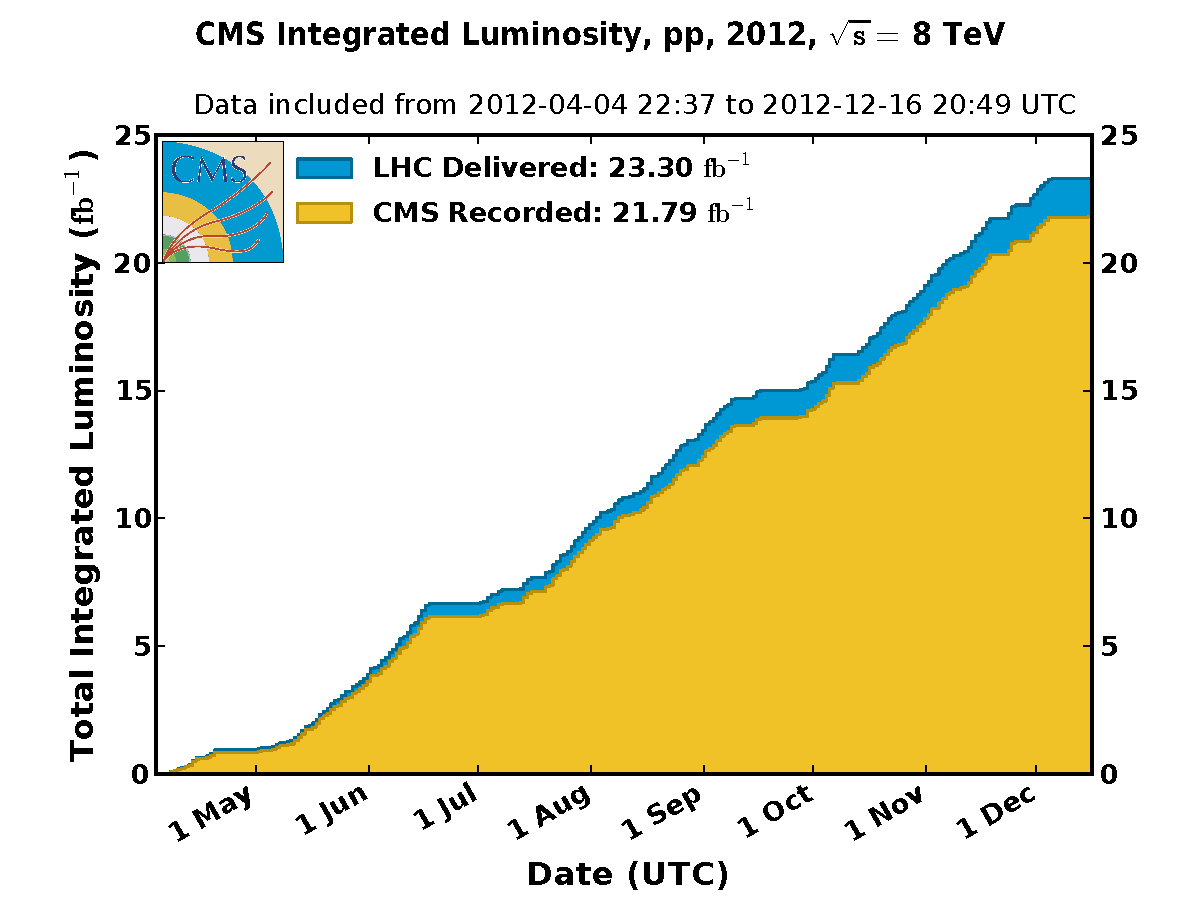
\includegraphics[width=\textwidth]{figures/2012_lumi.pdf}
    \caption{ The integrate luminosity per day delivered and recorded by CMS in
        2012. The flat periods in May, July, and September correspond to the
        boundaries between the run eras. }
    \label{fig:2012_luminosity}
\end{figure}

The data collected by CMS are split into smaller datasets based on the physics
objects contained within the events. This allows analyses to use only one or
two datasets, instead of requiring them to deal with the entirety of the CMS
data (which is petabyte scale, and hence too large for most institutes to store
locally). The HLT sorts events into the various datasets based on the triggers
that the event fired. In this manner, and event can end up in multiple datasets
if it fired multiple triggers. This analysis uses the \SingleElectron dataset
which was collected with the HLT trigger \SingleElectronTrigger. These datasets
were reconstructed---converted from raw detector response into physics
objects---in January, 2013, in order to make use of the most recent
calibrations derived from the entire 2012 run. A summary of the datasets used
are listed in \TAB~\ref{table:datasets}.

\begin{table}[h]
\centering
\begin{center}
    \begin{tabular}{ | l | c | c |}
    \hline
    Dataset Name                          & Run Range      & Luminosity       \\ \hline
    /SingleElectron/Run2012A-22Jan2013-v1 & 190456--193621 & $889.362 \pbinv$ \\ \hline
    /SingleElectron/Run2012B-22Jan2013-v1 & 193833--196531 & $4.429 \fbinv$   \\ \hline
    /SingleElectron/Run2012C-22Jan2013-v1 & 198022--203742 & $7.152 \fbinv$   \\ \hline
    /SingleElectron/Run2012D-22Jan2013-v1 & 203777--208686 & $7.318 \fbinv$   \\ \hline
    \end{tabular}
\end{center}
\caption{
    The datasets used in this analysis.
}
\label{table:datasets}
\end{table}

Although there is a \DoubleElectron dataset which uses a trigger designed to
find Z bosons, this analysis uses the \SingleElectron dataset selected with the
\SingleElectronTrigger trigger. The primary motivation behind using this
trigger was to allow a direct comparison with a similar \phistar analysis being
performed by CMS which used \Ztomumu events selected with a single muon
trigger. The single electron trigger requires an electron with $\pt > 27$ which
passes Working Point 80 (\WPEighty), a set of selection requirements on lepton
isolation and shower shape designed to be 80\% efficient on electrons. The
requirements that make up \WPEighty are listed in \TAB~\ref{table:wp80}. This
trigger had the lowest \pt threshold of any single electron trigger that was
unprescaled run during 2012. To prescale a trigger means to apply a rate
reduction by randomly throwing out a certain fraction of events in order to
keep the total trigger rate manageable; as this trigger was unprescaled, no
events were discarded in this manner.

\begin{table}[h]
\centering
\begin{center}
    \begin{tabular}{ | c | c c |} \hline
        Value                      & EB     & EE     \\ \hline
        $|\eta| <$                 & 1.4791 & 2.65   \\
        $\pt >$                    & 27     & 27     \\
        $\sigmaietaieta <$         & 0.1    & 0.03   \\
        $\ECALISO / \et <$         & 0.15   & 0.1    \\
        $\HOverE <$                & 0.1    & 0.05   \\
        $\HCALISO / \et <$         & 0.1    & 0.1    \\
        Pixel Matching $\ge$       & 1      & 1      \\
        $|\ooeoop| <$              & 0.05   & 0.05   \\
        $|\Delta \eta| <$          & 0.007  & 0.007  \\
        $|\Delta \phi| <$          & 0.06   & 0.03   \\ \hline
    \end{tabular}
\end{center}
\caption{
    The selection requirements for the \SingleElectronTrigger trigger for
    electrons which end up in the barrel region or the endcap region of ECAL.
    The variables used are detailed in \SEC~\ref{sec:electron_variables}.
}
\label{table:wp80}
\end{table}

The events from the \SingleElectron sample are further filtered for quality. A
centrally produced list of good luminosity segments is used to select only
events in which the part of the detector was malfunctioning or disabled. After
accounting for detector dead time and beam quality, \GoodLumiNumber of
integrated luminosity are used for physics analysis.

\subsection{Monte Carlo}
\label{ssec:monte_carlo}

This analysis makes use of numerous simulated data samples---colloquially
referred to as Monte Carlo (MC)---in order to estimate backgrounds and signal
yields, derive scale factors, and correct for the effects of bin migration on
the final measurement. All the MC used in this analysis were central generated
by the CMS collaboration. A \DYtoll signal sample and a $\ttbar\text{+jets}$
background sample were generated with \MADGRAPH \cite{alwall2014}. Diboson
($\Z\Z$, $\W\Z$, $\W\W$) background samples and a \DYtotautau background sample
were generated with \PYTHIA \cite{sjostran2006}. Background samples consisting
of $\tbar \W$ and $t \W$ were generated using \POWHEG
\cite{nason2004}\cite{alioli2010}\cite{re2011}. The details of these samples
are listed in \TAB~\ref{table:mc}.

\begin{table}[h]
\centering
\begin{center}
    \begin{tabular}{ | l | l c c |}
    \hline
    Process                                &  Generator & $\sigma$, pb  & Events $(\times 10^{6})$ \\ \hline
    \DYtoll                                &  \MADGRAPH & 3531.9 (NNLO) & 30.460 \\
    \DYtotautau                            &  \PYTHIA   & 1966.7 (\TODO{??})       & 3.297  \\
    \ttbar                                 &  \MADGRAPH & 23.64         & 3.984  \\
    $t \rightarrow \W+b \rightarrow X$     &  \POWHEG   & 11.1          & 0.498  \\
    $\tbar \rightarrow \W+b \rightarrow X$ &  \POWHEG   & 11.1          & 0.493  \\
    $\W\W$                                 &  \PYTHIA   & 54.84         & 10.000 \\
    $\W\Z$                                 &  \PYTHIA   & 33.21         & 10.000 \\
    $\Z\Z$                                 &  \PYTHIA   & 17.7          & 9.800  \\ \hline
    \end{tabular}
\end{center}
\caption{
    Summary of the MC samples used in this analysis. All cross sections are NLO
    unless otherwise stated. \TODO{Is pythia NLO?}
}
\label{table:mc}
\end{table}

After the generation step, MC is sent through a full detector simulation which
uses \GEANTfour \cite{agostinelli2003} to mimic the detector response. This
detector response is reconstructed using the full CMS reconstruction chain to
produce MC files that are in a format identical to actual data.

MC events have actual data events overlaid on top of them to better match the
conditions found in actual running. These overlaid events come from the minimum
bias dataset, which is selected with a minimum of conditions on order to select
events that are "typical" of proton-proton collisions. Additional events are
overlaid in order to simulate pileup. The number of pileup events overlaid is
drawn from a distribution that is expected to match the distribution seen in
data. Of course it is not possible to perfectly predict the data distribution
and so a reweighting technique is used to match the MC distribution to the
data. The distribution in MC is compared to that in data and a weight is
assigned to each MC event to force the distributions to match.

\section{Object Selection}

\subsection{Electron Selection}
\label{ssec:electron_selection}

The requirements used to select electrons offline are selected to be tighter
than the requirements used in the trigger in order to make calculating the
various efficiencies easier. For an event to be considered it must have at
least two electrons with $\pt > 20 \GeV$ and $|\eta| < 2.4$ which are the
looser bounds used in our acceptance. If three or more electrons pass this
initial requirement, only the two highest \pt electrons are considered. One of
these electrons must be within $|\eta| < 2.1$ and it must also have $\pt > 30
\GeV$.

There are several centrally defined ``cut based identification'' requirements
used in offline electron selection at CMS. We use two of these, referred to as
\EGMEDIUM and \EGTIGHT, with \EGTIGHT having stricter requirements than
\EGMEDIUM. The exact definition of these requirements are given in
\TAB~\ref{table:eg_cuts}.

\begin{table}[h]
\centering
\begin{center}
    \begin{tabular}{ | c | c  c | c  c |} \hline
        \multirow{2}{*}{Variable}     & \multicolumn{2}{c |}{\EGTIGHT}    & \multicolumn{2}{c |}{\EGMEDIUM} \\
                                      & EB        & EE        & EB        & EE \\ \hline
        $\detain <$                   & 0.004     & 0.005     & 0.004     & 0.007 \\
        $\dphiin <$                   & 0.03      & 0.02      & 0.06      & 0.03 \\
        $\sigmaietaieta <$            & 0.01      & 0.03      & 0.01      & 0.03 \\
        $\HOverE <$                   & 0.12      & 0.10      & 0.12      & 0.10 \\
        $d_{0} <$                     & 0.02      & 0.03      & 0.02      & 0.02 \\
        $d_{z} <$                     & 0.1       & 0.1       & 0.1       & 0.1 \\
        $|\ooeoop| <$                 & 0.05      & 0.05      & 0.05      & 0.05 \\
        $\pvtx <$                     & $10^{-6}$ & $10^{-6}$ & $10^{-6}$ & $10^{-6}$ \\
        $\nmiss \le$                  & 0         & 0         & 1         & 1 \\
        $\PFISO / \pt^{\text{e}} <$   & 0.10      & 0.10      & 0.15      & 0.15 \\ \hline
    \end{tabular}
\end{center}
\caption{
    Identification and isolation requirements for \EGTIGHT and \EGMEDIUM
    requirements in the ECAL barrel (EB) and ECAL endcap (EE).
    The variables used are detailed in \SEC~\ref{sec:electron_variables}.
}
\label{table:eg_cuts}
\end{table}

A \CentralElectron is required to pass \EGTIGHT and to be matched to one of the
electrons that passed \SingleElectronTrigger with $\Delta R < 0.3$. The other
electron must pass \EGMEDIUM. If both electrons are \CentralElectrons, then
only one of them need pass \EGTIGHT, but this same electron must also match the
trigger; the other \CentralElectron need only pass \EGMEDIUM.

No charge requirements are applied as even the same sign electron sample is
dominated by actual \Z decays as demonstrated by the large peak in the \mee
distribution.

\TODO{Plots: Electron plots: $\eta$, \pt}

\subsection{\Z Selection}

The \Z boson decays too quickly to leave any direct signal in the detector, so
it is reconstructed from its decay products: the two electrons whose selection
is described in \SEC~\ref{ssec:electron_selection}. In events where the two
electrons pass the selection, the \Z is constructed by taking the sum of the
electrons four-vectors. The resulting invariant mass of the \Z must be within
the region set by the acceptance (\MassRange).

\TODO{Plots: Z plots: \mee, Y, $Z_{\pt}$}

\section{Background Estimation}

The distribution of background events is estimated using the MC samples
discussed in \SEC~\ref{ssec:monte_carlo}, with the exception of QCD related
backgrounds, which are computed using data. The various MC samples are
reweighed so that they have equivalent luminosity to the data and the event
selection requirements are applied to them. The number of events that survive
the selection are taken as the number in our data, and are subtracted off from
the data events.

\begin{table}[h]
\centering
\begin{center}
    \begin{tabular}{ | l | r | r |}
    \hline
    Process           & of total & of background \\ \hline
    Signal: $\DYtoee$ &  99.53\% & N.A. \\ \hline
    \ttbar            &   0.14\% & 30.9\% \\ \hline
    $\Z\Z$            &   0.13\% & 27.2\% \\ \hline
    $\W\Z$            &   0.12\% & 25.9\% \\ \hline
    $\W\W$            &   0.03\% &  6.8\% \\ \hline
    $\DYtotautau$     &   0.03\% &  5.8\% \\ \hline
    $t\W + \tbar\W$   &   0.02\% &  3.4\% \\ \hline
    \end{tabular}
\end{center}
\caption{
    Data sample composition as a percentage of the total, as well as the
    backgrounds as a percentage of all background events.
    \TODO{Add QCD}
}
\label{table:bg_percentages}
\end{table}

Overall, the selection requirements discussed in the previous sections leave a
very pure sample of \Z boson events. 99.5\% of events are signal. The dominant
backgrounds are the diboson backgrounds and \ttbar. We define \Z bosons
produced in association another weak boson as a background because of their
different production mechanism as opposed to single \Z boson events. The
fraction of events from each of the considered backgrounds is listed in
\TAB~\ref{table:bg_percentages}

\subsection{QCD Background Estimation}

The centrally produced QCD MC does not have enough events to make an accurate
estimation of the QCD background in this analysis so instead a data driven
method is employed. The same requirements as discussed in
\SEC~\ref{ssec:electron_selection} are applied to both the data and the MC
samples with the additional requirement that both electrons must have the same
sign. The MC samples are then weighted to match the luminosity of the data and
their events are subtracted. The remaining events still have a large
contribution from the \Z (see \FIG~\ref{fig:same_sign_z_peak}) and so we reject
events that fall within the \mee acceptance region of \MassRange.
\TODO{Are we just taking this number, or do we fit and integrate?}

\TODO{Same sign \mee peak plot before and after subtraction.
\label{fig:same_sign_z_peak}}

\chapter{Analysis}
\label{chapter:analysis}

\section{Uncertainties}
\label{sec:uncertainties}

\TODO{Intro?}

\subsection{Statistical Uncertainties}
\label{ssec:stat_uncertainty}

The statistical uncertainties due to the number of data events are propagated
through the unfolding method, as discussed in
\SEC~\ref{ssec:unfolding_statistical_uncertainties}. For the normalized cross
section measurement, this uncertainty is corrected for the uncertainty on the
total cross section as follows:

\TODO{Understand this formula...}
\begin{equation} \label{eq:stat}
    \left( \errnorm_{i} \right)^{2}
    =
    \left[
    \errabs_{i} \cdot
        \left(
            \frac{1}{\sigma} - \frac{1}{\sigma^{2}}
        \right)
    \right]^{2}
    +
    \sum_{i \ne j}
    \left(
        \errabs_{j} \cdot \frac{1}{\sigma^{2}}
    \right)^{2}
\end{equation}

where $\errnorm_{i}$ is the statistical uncertainty for normalized bin $i$,
$\errabs_{j}$ is the statistical uncertainty for bin $j$ in the absolute
distribution, and $\sigma$ is the overall cross section given by the integral
of the absolute distribution. The correction yielded by this formula is small.

The statistical uncertainty ranges from 0.26 to 1.21\% for both the absolute
and normalized cross section measurement. It is one of the dominant
uncertainties for the normalized cross section measurement.

\subsection{Statistical Uncertainties from the Monte Carlo Samples}
\label{ssec:mc_stat_uncertainty}

The \MADGRAPH signal MC sample has fewer events which pass our final selection
than there are events in the data. This sample is used to unfold the data and
so its statistical uncertainty affects the final measurement. The affect of the
statistical uncertainty on the bin migration matrix is propagated through to
the final result via the use of toy MC, detailed in
\SEC~\ref{ssec:unfolding_statistical_uncertainties}. The uncertainty found with
this method is 0.1 to 0.2\% for both the absolute and normalized cross section
measurements.

In addition to affecting the unfolding, the low number of events in the MC
affects the efficiency correction discussed in \SEC~\ref{ssec:eff_correction}
and shown in \FIG~\ref{fig:average_efficiencies}. These uncertainties vary from
0.3 to 1.3\% for both the absolute and normalized cross section measurements.

These two sources of uncertainty are measured separately. The finally
uncertainty due to the statistical uncertainties from the \MADGRAPH signal MC
sample is the sum in quadrature of both sources. This combined uncertainty is
the dominant uncertainty for the normalized cross section measurement, having a
slightly larger effect in each \phistar bin than the statistical uncertainty
due to the data.

\subsection{Luminosity Uncertainty}
\label{ssec:lumi_uncertainty}

The integrated luminosity is measured at CMS using the occupancy in the
pixel detector during minimum-bias events \cite{cms_lumi_2013}. This luminosity
measurement is calibrated by using van der Meer scans---a method to measure the
beam size in which the two beams are displaced and then ``swept'' across each
other as the offset is reduced \cite{vandermeer_1968}.

The integrated luminosity for the run period considered in this analysis is
known to \LumiUncertainty. This uncertainty is taken to be fully correlated
bin-by-bin in \phistar for the absolute cross section measurement, where it is
by far the dominant uncertainty. The luminosity cancels in the normalized
cross section measurement and so the uncertainty only affects the background
subtraction. This effect is negligible compared to the uncertainty already
present due to the background subtraction, which is discussed in
\SEC~\ref{ssec:background_subtraction_uncertainty}. The large uncertainty on
the luminosity is the primary motivation behind making a normalized cross
section measurement.

\subsection{Pileup Uncertainty}
\label{ssec:pileup_uncertainty}

As discussed in \SEC~\ref{ssec:monte_carlo}, the high beam intensity at the LHC
leads to multiple proton-proton interactions at each bunch crossing. This is
modeled in MC by overlaying multiple simulated minimum-bias events on top of
each simulated event. The distribution of pileup in MC is reweighted to match
the data distribution based on the calculated instantaneous luminosity and the
inelastic proton-proton cross section. The uncertainty due to this reweighting
process is calculated by varying the inelastic cross section by plus and minus
5\%, recalculating the data distribution of pileup, and reweighting to the MC
samples to match this new distribution. The full analysis is then performed
with these MC samples and the differences between the \phistar distributions is
taken as a systematic uncertainty. The pileup uncertainty for the absolute
cross section measurement ranges from 0.21 to 0.58\%, while the uncertainty for
the normalized cross section measurement is between $< 0.01$ and 0.64\%.

\subsection{Trigger, Reconstruction, and Identification Scale Factors Uncertainty}
\label{scale_factor_uncertainty}

Differences between the MC and data are corrected for using scale factors.
Three different sets of scale factors are used to reweight the MC samples:
trigger scale factors (discussed in \SEC~\ref{ssec:sf_trigger}), reconstruction
scale factors (discussed in \SEC~\ref{ssec:sf_reconstruction}), and
identification scale factors (discussed in \SEC~\ref{ssec:sf_id}).

In all three cases, the uncertainties on the scale factors are propagated
through to the final measurement using 500 toy MC variations. In this method,
every toy is constructed by drawing each scale factor from a Gaussian
probability distribution with its mean set to nominal value of the scale factor
and its width set to the quadrature sum of the uncertainties on the scale
factor. Each toy is then used to weight the MC samples used in this analysis,
and the full analysis is performed with that newly weighted sample. The
uncertainty on the final result due to one of the three types of scale factors
is taken to be defined by the central 68.2\% of results from the toys.

This procedure for propagating the uncertainty is performed independently for
each of the three types of scale factors. The total uncertainty due to the
scale factors is the sum in quadrature of the three results. For the absolute
cross section measurement this uncertainty is about 0.4\%, while for the
normalized cross section measurement it ranges from 0.02 to 0.35\%.

\subsection{\texorpdfstring{\pt}{PT} Scale Uncertainty}
\label{ssec:pt_scale_uncertainty}

One of the advantages of the \phistar variable is that it is not computed using
the momentum of the electrons and instead uses only the angles between them,
which are generally better measured. This makes \phistar less sensitive to any
potential problems with the \pt measurement of electrons.

However, the measurement of the \pt of the electrons is used to determine which
events are included in our sample. Therefore, a shift in the \pt scale of the
detector will either add or remove events that have electrons near the \pt
selection requirement boundaries. To determine the uncertainty due to the \pt
scale, we vary the \pt values of all of the electron up and down by 0.3\%,
which is a conservative estimate of the uncertainty on the \pt scale. The
largest difference in each \phistar bin between the nominal result and the
results with the modified \pt scale is taken as the uncertainty in that bin.
The uncertainty due to the \pt scale for the absolute cross section measurement
is 0.07 to 0.17\%, while the uncertainty for the normalized cross section
measure is $< 0.01$ to 0.10\%.

\subsection{Background Subtraction Uncertainty}
\label{ssec:background_subtraction_uncertainty}

The background subtraction, which is discussed in \SEC~\ref{sec:background},
deals with three separate categories of backgrounds. The uncertainty in
each category is determined with a different method, and these uncertainties
are added in quadrature to determine the total uncertainty due to the
background subtraction.

The first category consists of the various backgrounds with two independent
decay chains each of which can produce a lepton: $\ttbar$, $\W\W$,
$\DYtotautau$, $t\W$, and $\tbar\W$. The contributions from these backgrounds
are estimated by using an \emu control sample as discussed in
\SEC~\ref{ssec:emu_sample}. The uncertainty from the scale factors derived
using this method are propagated through to the final result using 500 toy MC
variations. For each variation, the scale factors are randomly drawn from a
Gaussian distribution with mean equal to the nominal value of that scale factor
and width equal to the uncertainty on the scale factor. Each toy is then used
to weight the background MC samples and the full which are then used to perform
the background subtraction. The full analysis is then run with the newly
background-subtracted data samples. The uncertainty due to the subtraction of
this category of background for each bin in \phistar is defined by the spread
of the central 68.2\% values obtained by the toys.

The second category consists of the backgrounds with a real \Z boson: $\Z\Z$
and $\W\Z$. For these samples, the uncertainty is calculated by taking a
correlated 20\% uncertainty on the theoretical cross section.

The third and final category consists of the \QCDjets and \wjets
backgrounds. The method of estimating this background is discussed in
\SEC~\ref{ssec:qcd_background}. Instead of taking the uncertainties from the
fit, which would not account for any systematics in the method used, a
conservative 100\% uncertainty is assigned to this category.

The uncertainty due to the background subtraction for the absolute cross
section measurement varies from 0.02 to 0.64\%, and from 0.03 to 0.59\% in the
normalized cross section measurement.

\subsection{PDF and Cross Section Uncertainties}
\label{ssec:pdf_uncertainties}

As discussed in \TODO{\SEC~\ref{} Link to theory section}, the kinematics of
the \Z boson depend on the internal composition and kinematics of the protons
as they collide. The reconstructed \phistar distribution is therefore dependent
on the PDFs used to generate the signal MC sample.

The uncertainty due to this choice of PDF is calculated following the
recommendation of \PDFforLHC working group for the \POWHEG MC signal sample.
\PDFWeightProducer is used to reweight the \POWHEG sample using the \CTten PDF
set. A total of \num{26} different pairs of weights are used by the tool to
fully account for the uncertainty inherent in the PDF set; these weights are
provided by the \CTten collaboration specifically for this purpose. Each pair
of weights consists of a variation of a PDF parameter, with one weight
corresponding to adjusting the parameter up and the other weight to down. Each of
these weights are used to reweight the \POWHEG sample, and the analysis is
performed with this newly weighted sample.
The uncertainty due to each weight is taken to be the difference with the
nominal \phistar distribution. Two uncertainties are calculated: the
one due to all of the upward parameter adjustments, and one to all the downward
parameter adjustments added in quadrature. The largest of these for each
\phistar bin is taken as the total uncertainty.

For the \MADGRAPH MC signal sample, which is an LO sample generated with a LO
PDF, the uncertainties can not be calculated in this manner. Instead, the PDF
includes an uncertainty on the cross section as calculated by \FEWZ which is
used to scale the sample. This uncertainty is propagated through the analysis
be reweighting the \MADGRAPH with this uncertainty both added and subtracted.
The difference in the final \phistar distribution is taken as the uncertainty
due to the \FEWZ cross section. This uncertainty is the dominant uncertainty
from the \MADGRAPH sample.

\subsection{Final State Radiation Uncertainties}
\label{ssec:fsr_uncertainties}

FSR, where an electron radiates a photon, is discussed in
\SEC~\ref{sec:electron_dressing}. These photons can affect the reconstruction
of the \Z, but this is taken into account during the unfolding as discussed in
\SEC~\ref{sec:unfolding}. Hence, uncertainties in the modeling of FSR affect
the unfolding and the final measurement.

The uncertainty is calculated using the \FSRWeightProducer, which augments the
\PYTHIA QED calculation with exact $\BigO{\alpha}$ and $\alpha(\pt^{2})$
couplings and reweights the MC sample as if it had been produced with these
calculations from the start. The effect of this reweighting on the final
\phistar distribution is $\le 0.34\%$ for the absolute cross section
measurement and $\le 0.03\%$ for the normalized cross section measurement.

%\subsection{Electron Angular Position Uncertainty}
%
%\TODO{What has Nicole seen in new tests?}
%
%Since \phistar depends on the angles between the two electrons, it is sensitive
%to mismeasurement of these angles. As discussed in
%\SEC~\ref{sec:electron_reconstruction}, the position of a reconstructed
%electron comes from the tracker, and therefore misalignment of the tracker
%would lead to a systematic uncertainty on the angle measurement. The magnitude
%of this systematic is estimated by using the position of the ECAL supercluster
%associated with the electron to calculate the electron's position instead of
%using the track. The new supercluster-only position is then used to calculate a
%new \phistarSC that does not depend on the alignment of the tracker.
%
%The position of the supercluster does not take into account the amount the
%bending of the electron due to the magnetic field. While $\eta$ is unchanged by
%the pretense of the field, $\phi$ is changed. A correction is applied to $\phi$
%to find the angle at the interaction point, $\phizero$, based on the angle of
%the supercluster, $\phisc$. This correction is given by
%\EQ~\ref{eq:b_field_correction} where $q$ is the charge of the electron, \pt is
%the transverse momentum of the electron, $B$ is the magnitude of the magnetic
%field, and \Reffective is the effective radius of ECAL as a function of $\eta$
%and $\theta$ as given in \EQ~\ref{eq:effective_radius}. The charge and momentum
%come from the electron matched to the supercluster, and although they are
%determined in combination with the tracker, they are far less susceptible to
%the small scale misalignments of the tracker that we are considering.
%
%\begin{equation}\label{eq:b_field_correction}
%    \sin \left( \phisc - \phizero \right)
%    =
%    - \Reffective \frac{q B}{2 \pt}
%\end{equation}
%
%\begin{equation}\label{eq:effective_radius}
%    \Reffective
%    =
%    \left\{
%        \begin{array}{ll}
%            1.29 \meters & \text{if } |\eta| < 1.4442 \\
%            3.14 \meters \times \tan \left(\coord{\theta}\right) & \text{otherwise}
%        \end{array}
%    \right.
%\end{equation}
%
%The resulting \phistarSC distribution is compatible within statistical
%uncertainties with the \phistar distribution and so no systematic uncertainty
%is assigned for the angular position.
%
%\TODO{Plot of \phistar vs \phistarSC?}

\subsection{Uncertainty from Four Vector Corrections}
\label{four_vector_uncertainty}

The \mee distribution in the \MADGRAPH signal MC sample does not precisely
match the distribution in data, as seen in \FIG~\ref{fig:z_mass}. This
discrepancy remains even after applying the various energy and momentum
corrections to the electrons discussed in \SEC~\ref{sec:corrections}. In order
to determine the effect this has on the final measurement, the \MADGRAPH signal
MC sample is reweighted to remove this difference. The ratio between the
nominal \phistar value and the value derived after this reweighting is shown in
\FIG~\ref{fig:z_mass_reweighted}. The circular points show the ratio of the
reconstructed \phistar distributions, while the square points show the ratio of
the generated \phistar distributions. The errors are binomial. Most of the
points are consistent with \num{1}, and so no systematic uncertainty is
assigned for this disagreement.

\begin{figure}[!htbp]
    \centering
    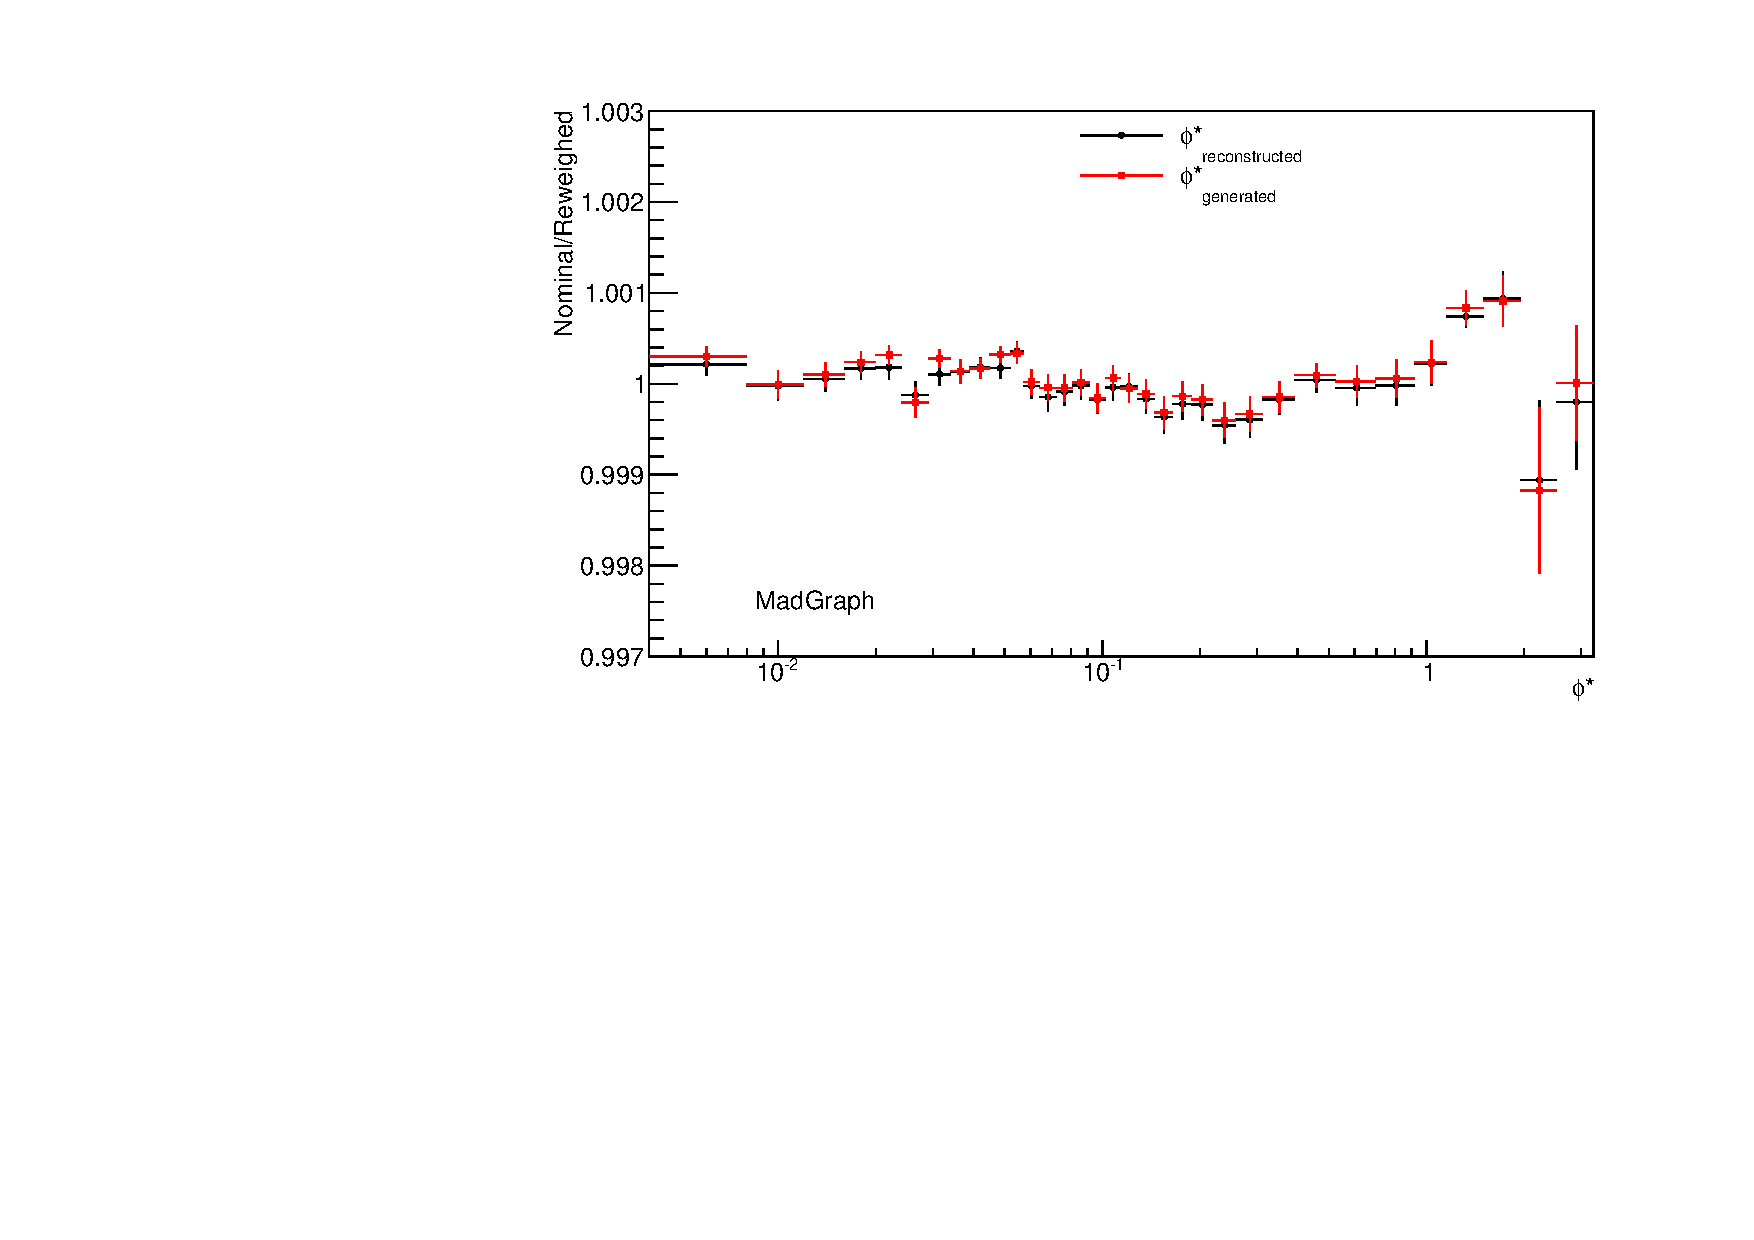
\includegraphics[width=\textwidth]{figures/ZMass_reweighed.pdf}
    \caption[
        The ratio of \phistar in \MADGRAPH before and after reweighting to
        remove the differnce in the \mee distribution between MC and data.
    ]{
        The ratio of \phistar in \MADGRAPH before and after reweighting to
        remove the difference in the \mee distribution between MC and data seen
        in \FIG~\ref{fig:z_mass}. The circular points are the ratio in the
        reconstructed quantity, while the square points are the ratio in the
        generated quantity. The uncertainties are binomial.
    }
    \label{fig:z_mass_reweighted}
\end{figure}

Likewise, the \Z \rapidity distribution in \MADGRAPH does not match the
distribution in data, as seen in \FIG~\ref{fig:z_rapidity}. The same
reweighting procedure as is performed for the \mee case above is used here to
force the distributions to agree. The ratio between the nominal \phistar value
and the value derived after this reweighting is shown in
\FIG~\ref{fig:z_mass_reweighted}.
The circular points show the ratio of the
reconstructed \phistar distributions, while the square points show the ratio of
the generated \phistar distributions. The disagreement is on the order of
0.05\% for most of the distribution, increasing to 0.4--0.5\% in the highest
\phistar bins. Although this is larger than the effect seen in the \mee
reweighting, it is much smaller than the statistical uncertainties and so is
not included in the final results.

\begin{figure}[!htbp]
    \centering
    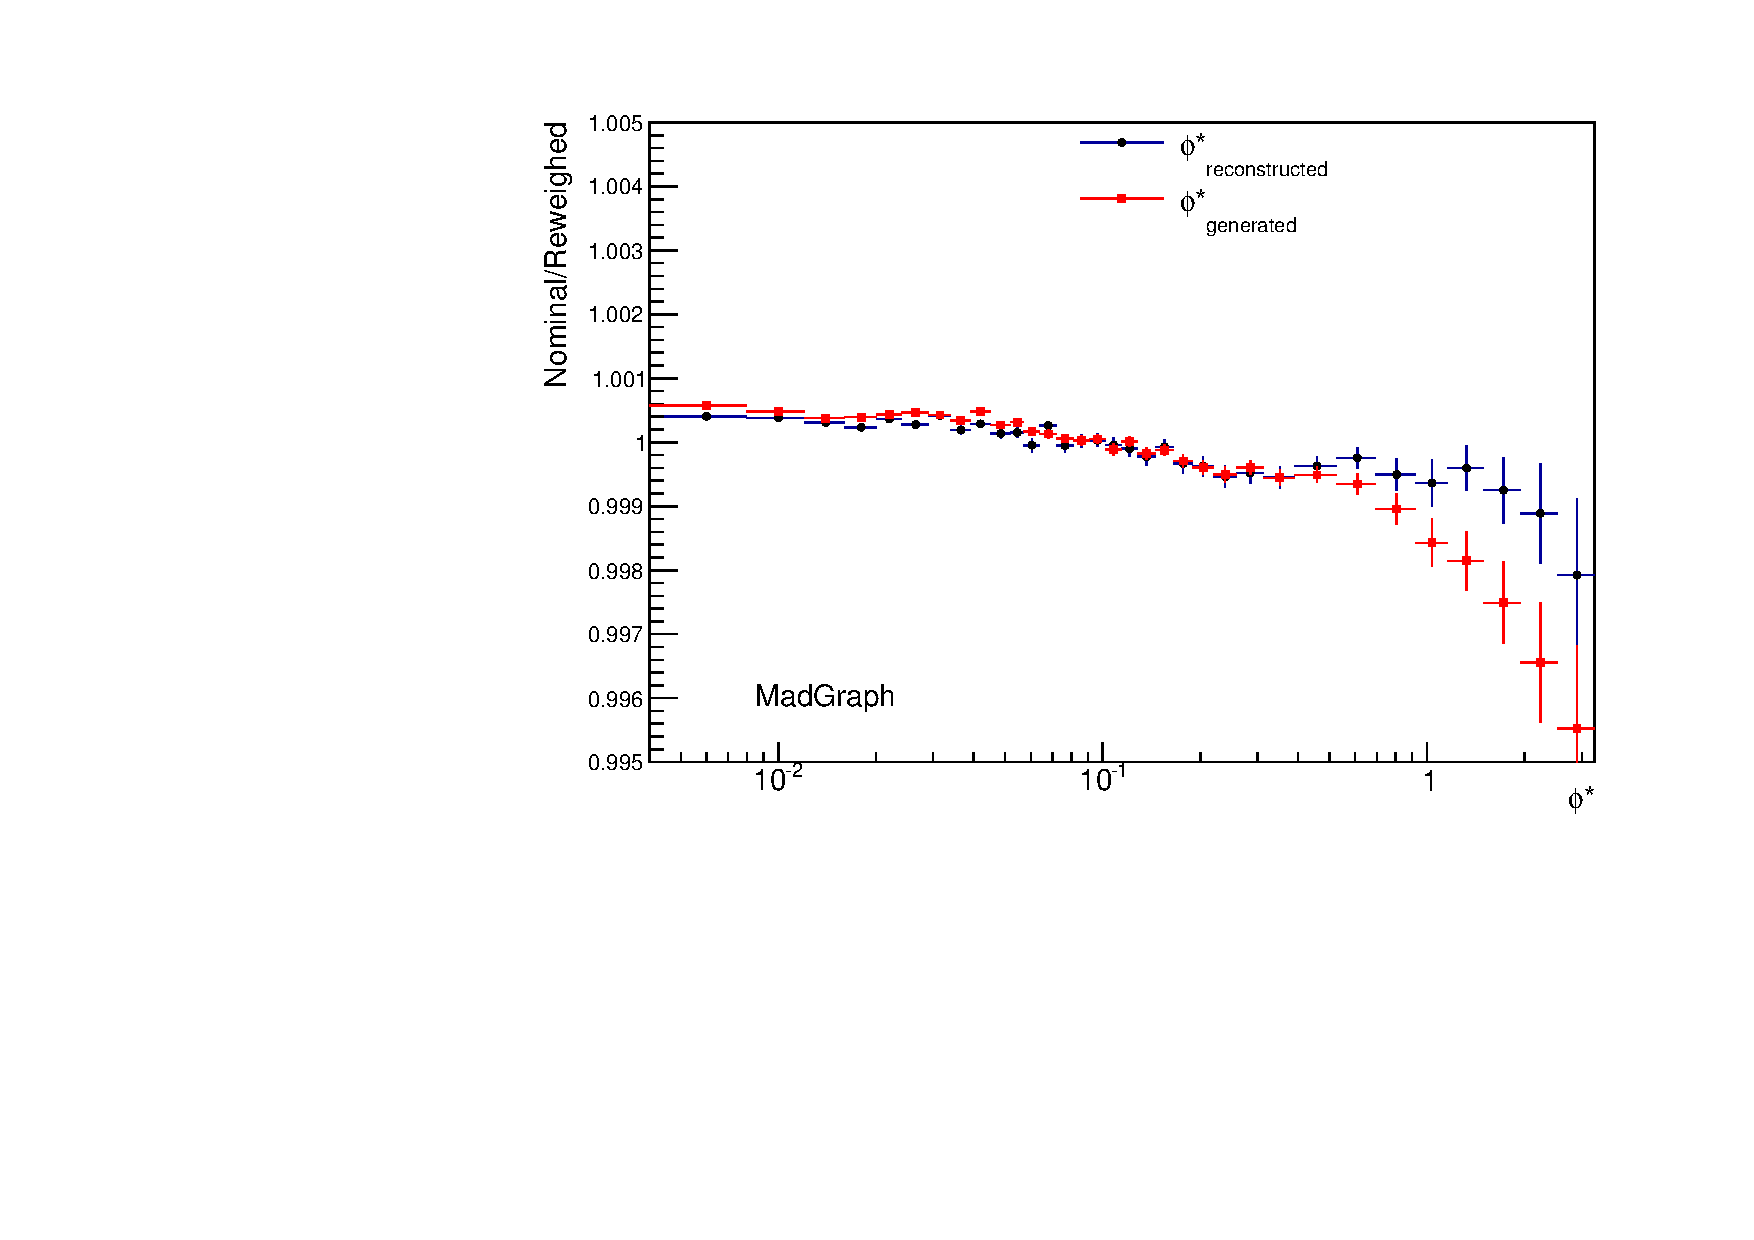
\includegraphics[width=\textwidth]{figures/ZY_reweighed.pdf}
    \caption[
        The ratio of \phistar in \MADGRAPH before and after reweighting to
        remove the differnce in the \rapidity distribution between MC and data.
    ]{
        The ratio of \phistar in \MADGRAPH before and after reweighting to
        remove the difference in the \rapidity distribution between MC and data
        seen in \FIG~\ref{fig:z_rapidity}. The circular points are the ratio in
        the reconstructed quantity, while the square points are the ratio in
        the generated quantity. The uncertainties are binomial.
    }
    \label{fig:z_mass_reweighted}
\end{figure}

\section{Uncertainty Figures}

The values of the various uncertainty in each \phistar bin are presented in the
figures that follow. Figure~\ref{fig:sys_uncert_abs} shows the fractional
uncertainty in the absolute \phistar cross section in data unfolded with
\MADGRAPH while \FIG~\ref{fig:sys_uncert_abs_powheg} shows the fractional
uncertainty in data unfolded with \POWHEG. The uncertainty on the absolute
\phistar cross section in \MADGRAPH and \POWHEG are shown in
\FIGS~\ref{fig:madgraph_uncert_abs} and \ref{fig:powheg_uncert_abs},
respectively. Figure~\ref{fig:sys_uncert_norm} shows the fractional uncertainty
in the normalized \phistar cross section in data unfolded with \MADGRAPH while
\FIG~\ref{fig:sys_uncert_norm_powheg} shows the fractional uncertainty in the
data unfolded with \POWHEG. The uncertainty on the normalized \phistar cross
section in \MADGRAPH and \POWHEG are shown in
\FIGS~\ref{fig:madgraph_uncert_norm} and \ref{fig:powheg_uncert_norm},
respectively. All of these values are presented in tables in
\APP~\ref{app:uncertainty_tables}.

% Absolute

% fig:sys_uncert_abs
\begin{figure}[!p]
    \centering
    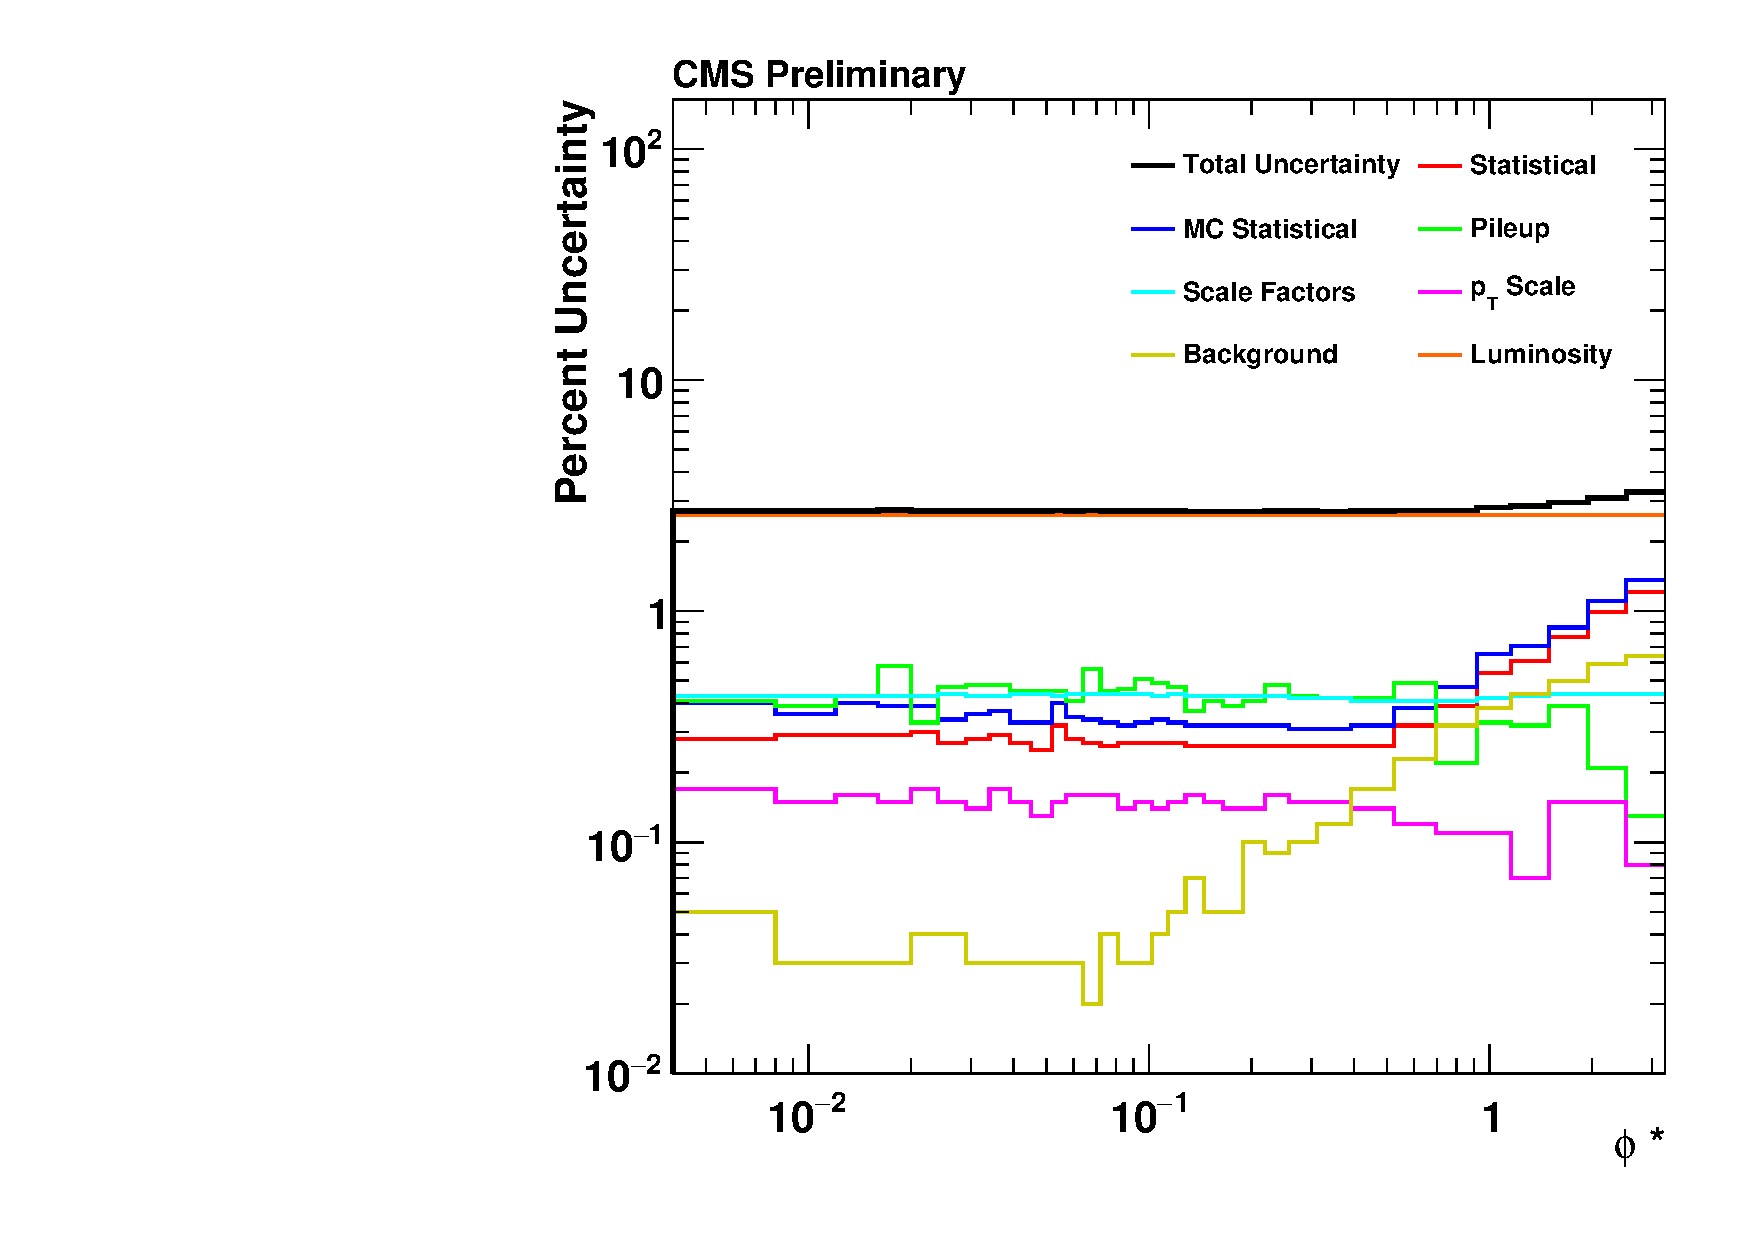
\includegraphics[width=\textwidth]{figures/data_uncertainty_absolute.pdf}
    \caption[
        Fractional errors (in \%) for the absolute cross section measurement
        made with data unfolded with \MADGRAPH.
    ]{
        Fractional errors (in \%) for the absolute cross section measurement
        made with data unfolded with \MADGRAPH. The total value is the sum in
        quadrature of all the other values. These uncertainties are also
        presented in tabular form in \cref{tab:sys_uncert_abs}.
    }
    \label{fig:sys_uncert_abs}
\end{figure}


% fig:sys_uncert_abs_powheg
\begin{figure}[!p]
    \centering
    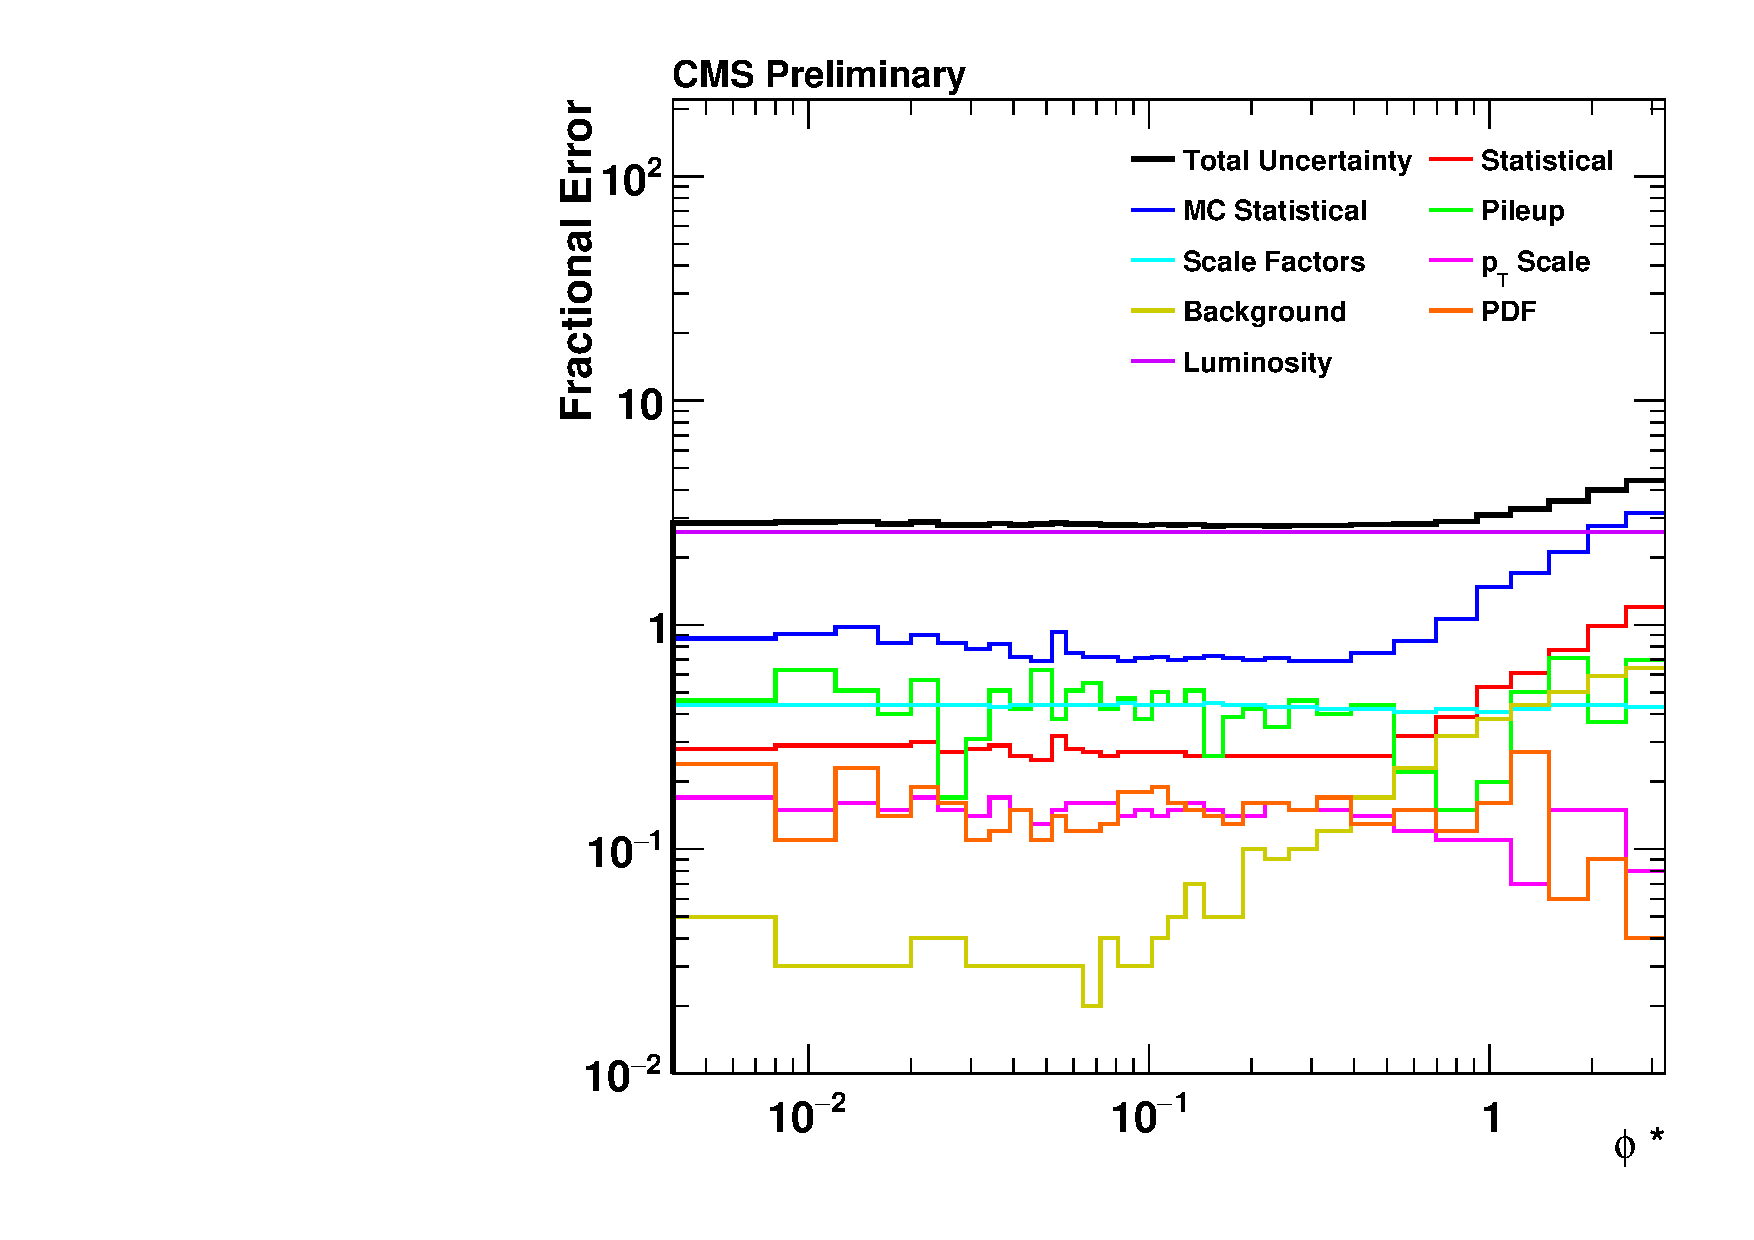
\includegraphics[width=\textwidth]{figures/data_uncertainty_absolute_powheg_unfolded.pdf}
    \caption[
        Fractional errors (in \%) for the absolute cross section measurement
        made with data unfolded with \POWHEG.
    ]{
        Fractional errors (in \%) for the absolute cross section measurement
        made with data unfolded with \POWHEG. The total value is the sum in
        quadrature of all the other values. These uncertainties are also
        presented in tabular form in \cref{tab:sys_uncert_abs_powheg}.
    }
    \label{fig:sys_uncert_abs_powheg}
\end{figure}


% fig:madgraph_uncert_abs
\begin{figure}[!htbp]
    \centering
    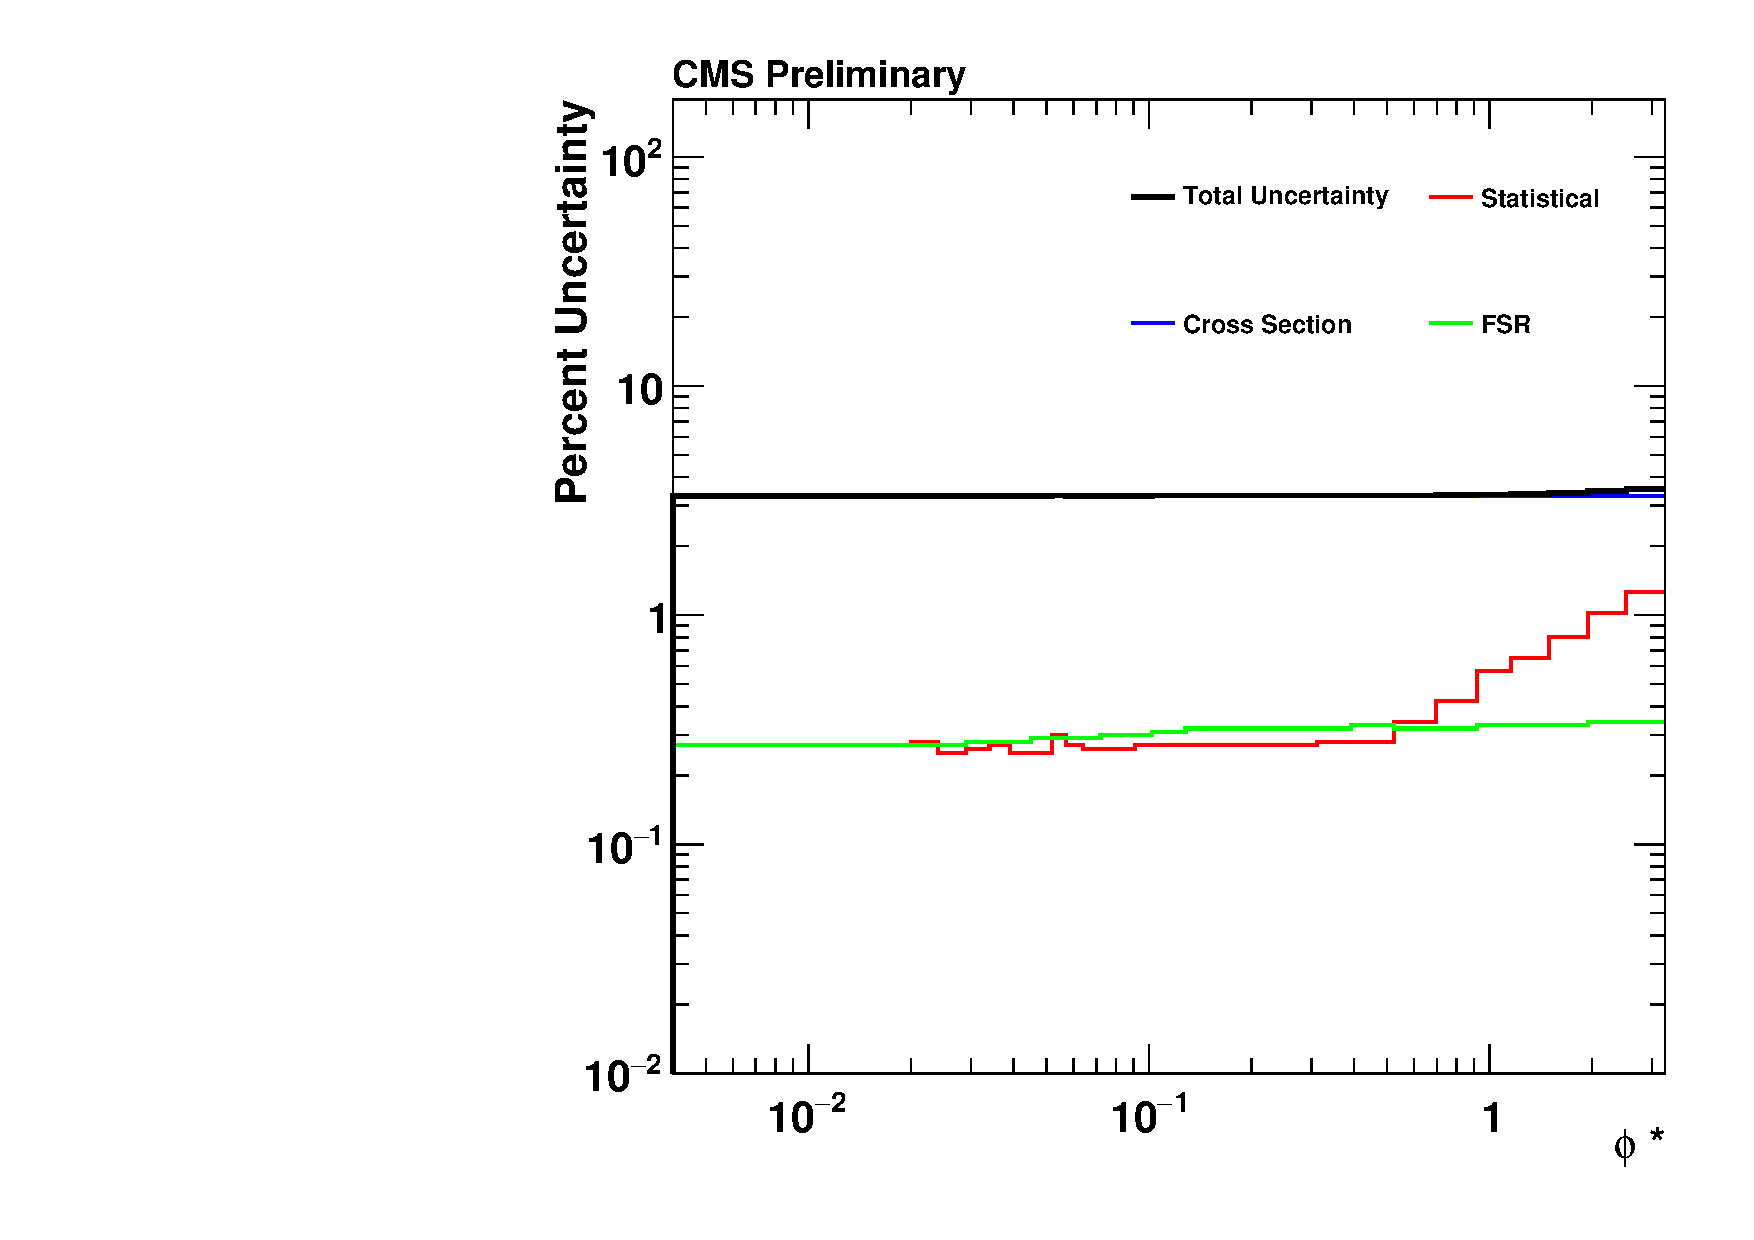
\includegraphics[width=\textwidth]{figures/madgraph_uncertainty_absolute.pdf}
    \caption[
        Fractional errors (in \%) for the absolute cross section from the
        \MADGRAPH MC sample.
    ]{
        Fractional errors (in \%) for the absolute cross section from the
        \MADGRAPH MC sample. These uncertainties are also presented in tabular
        form in \TAB~\ref{tab:madgraph_uncert_abs}.
    }
    \label{fig:madgraph_uncert_abs}
\end{figure}


% fig:powheg_uncert_abs
\begin{figure}[!p]
    \centering
    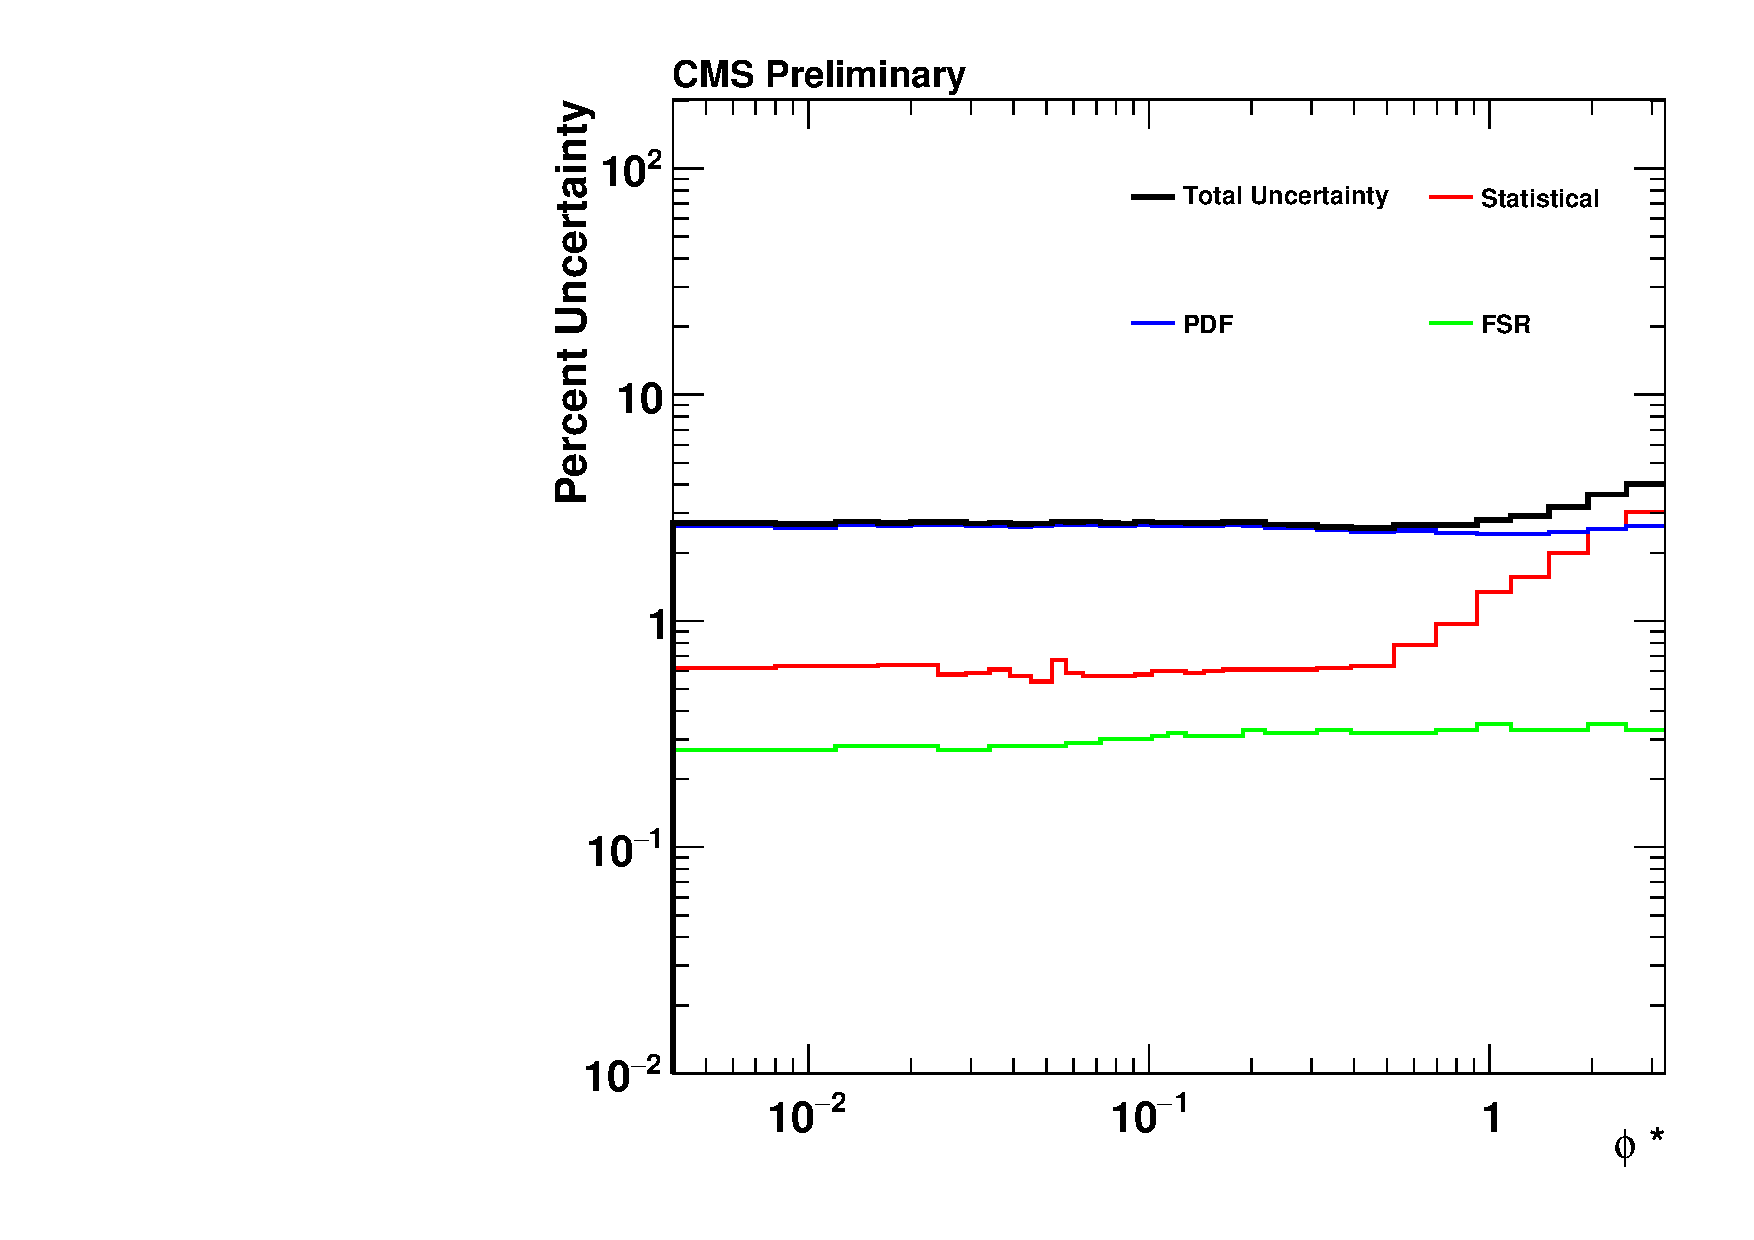
\includegraphics[width=\textwidth]{figures/powheg_uncertainty_absolute.pdf}
    \caption[
        The uncertainties for the absolute cross section from the \POWHEG MC
        sample.
    ]{
        The uncertainties (in \%) for the absolute cross section from the
        \POWHEG MC sample. These uncertainties are also presented in tabular
        form in \cref{tab:powheg_uncert_abs}.
    }
    \label{fig:powheg_uncert_abs}
\end{figure}


% Normalized

% fig:sys_uncert_norm
\begin{figure}[!p]
    \centering
    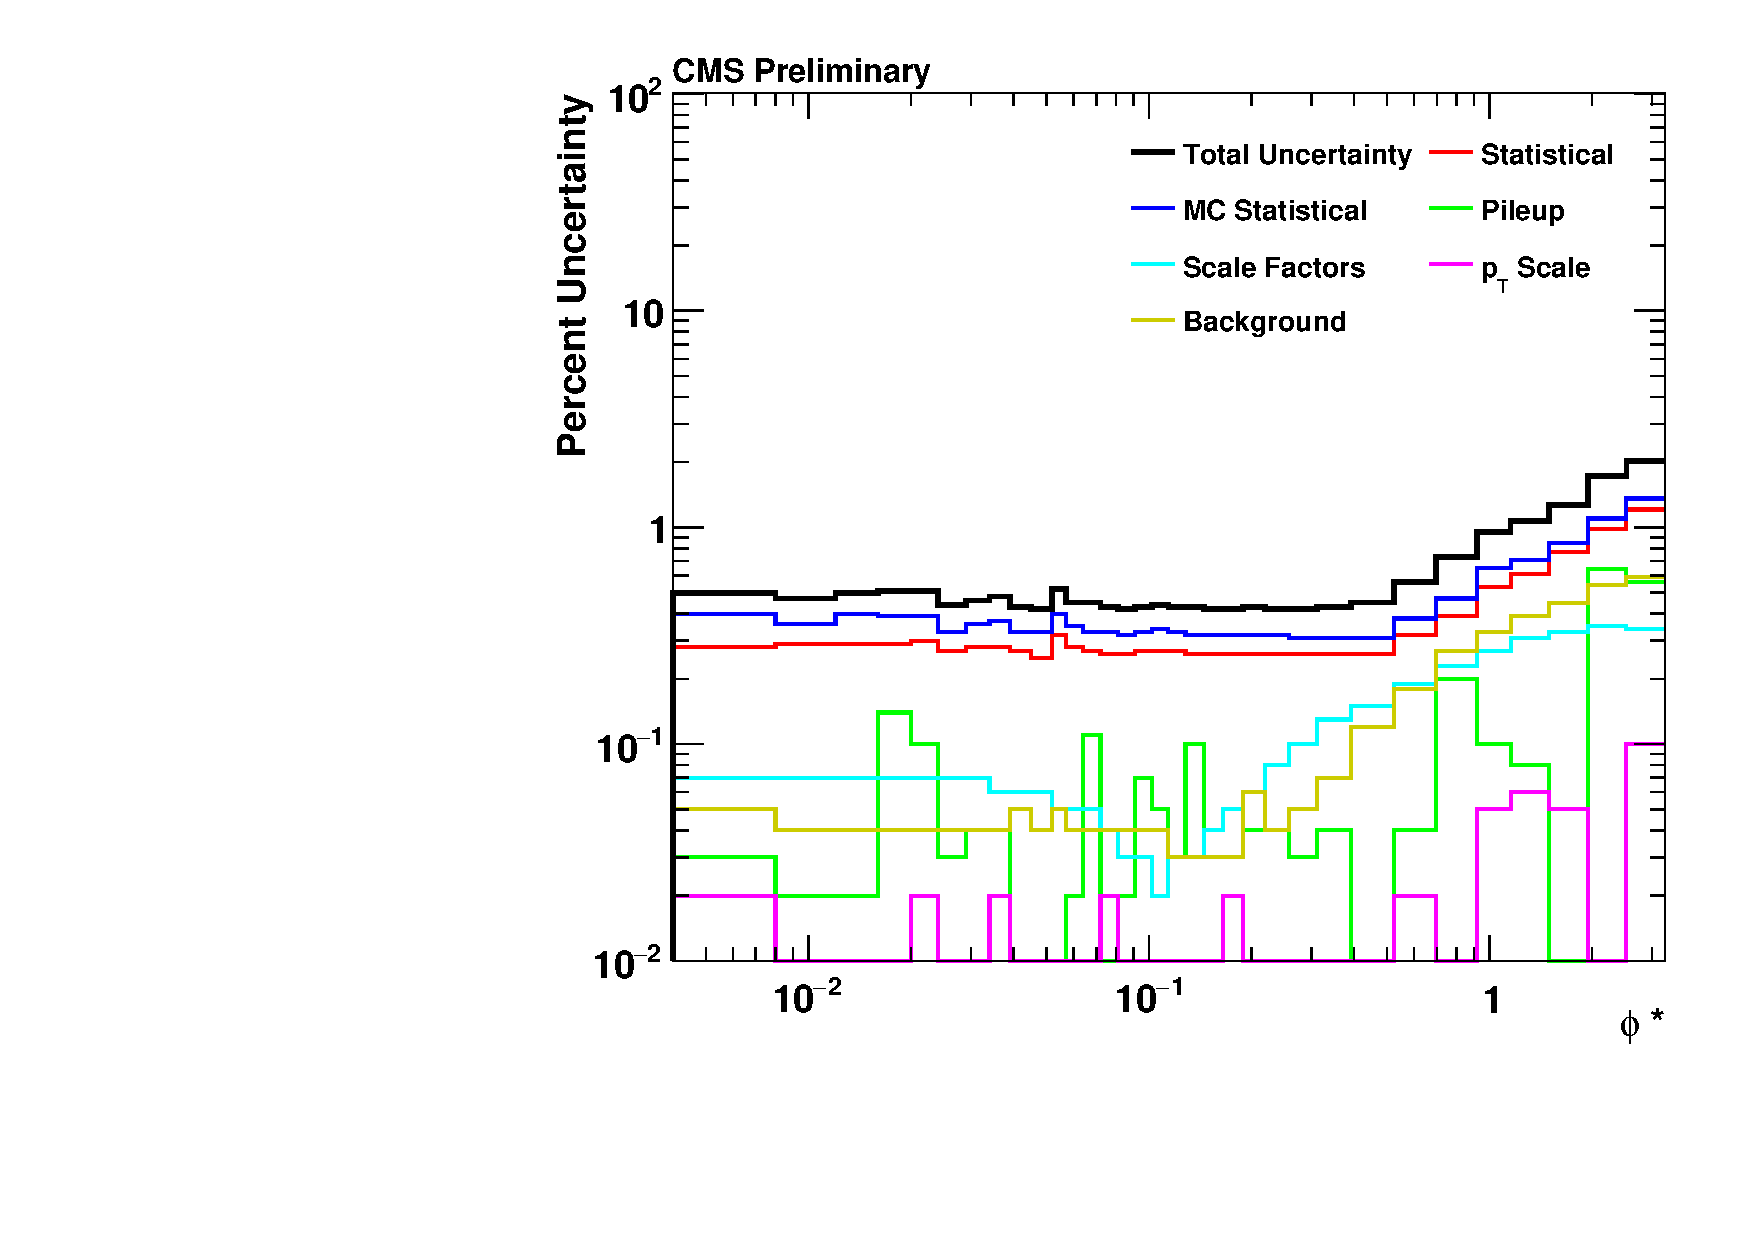
\includegraphics[width=\textwidth]{figures/data_uncertainty_normalized.pdf}
    \caption[
        Fractional errors for the normalized cross section measurement
        made with data unfolded with \MADGRAPH.
    ]{
        Fractional errors (in \%) for the normalized cross section measurement
        made with data unfolded with \MADGRAPH. The total value is the sum in
        quadrature of all the other values. These uncertainties are also
        presented in tabular form in \cref{tab:sys_uncert_norm}.
    }
    \label{fig:sys_uncert_norm}
\end{figure}


% fig:sys_uncert_norm_powheg
\begin{figure}[!p]
    \centering
    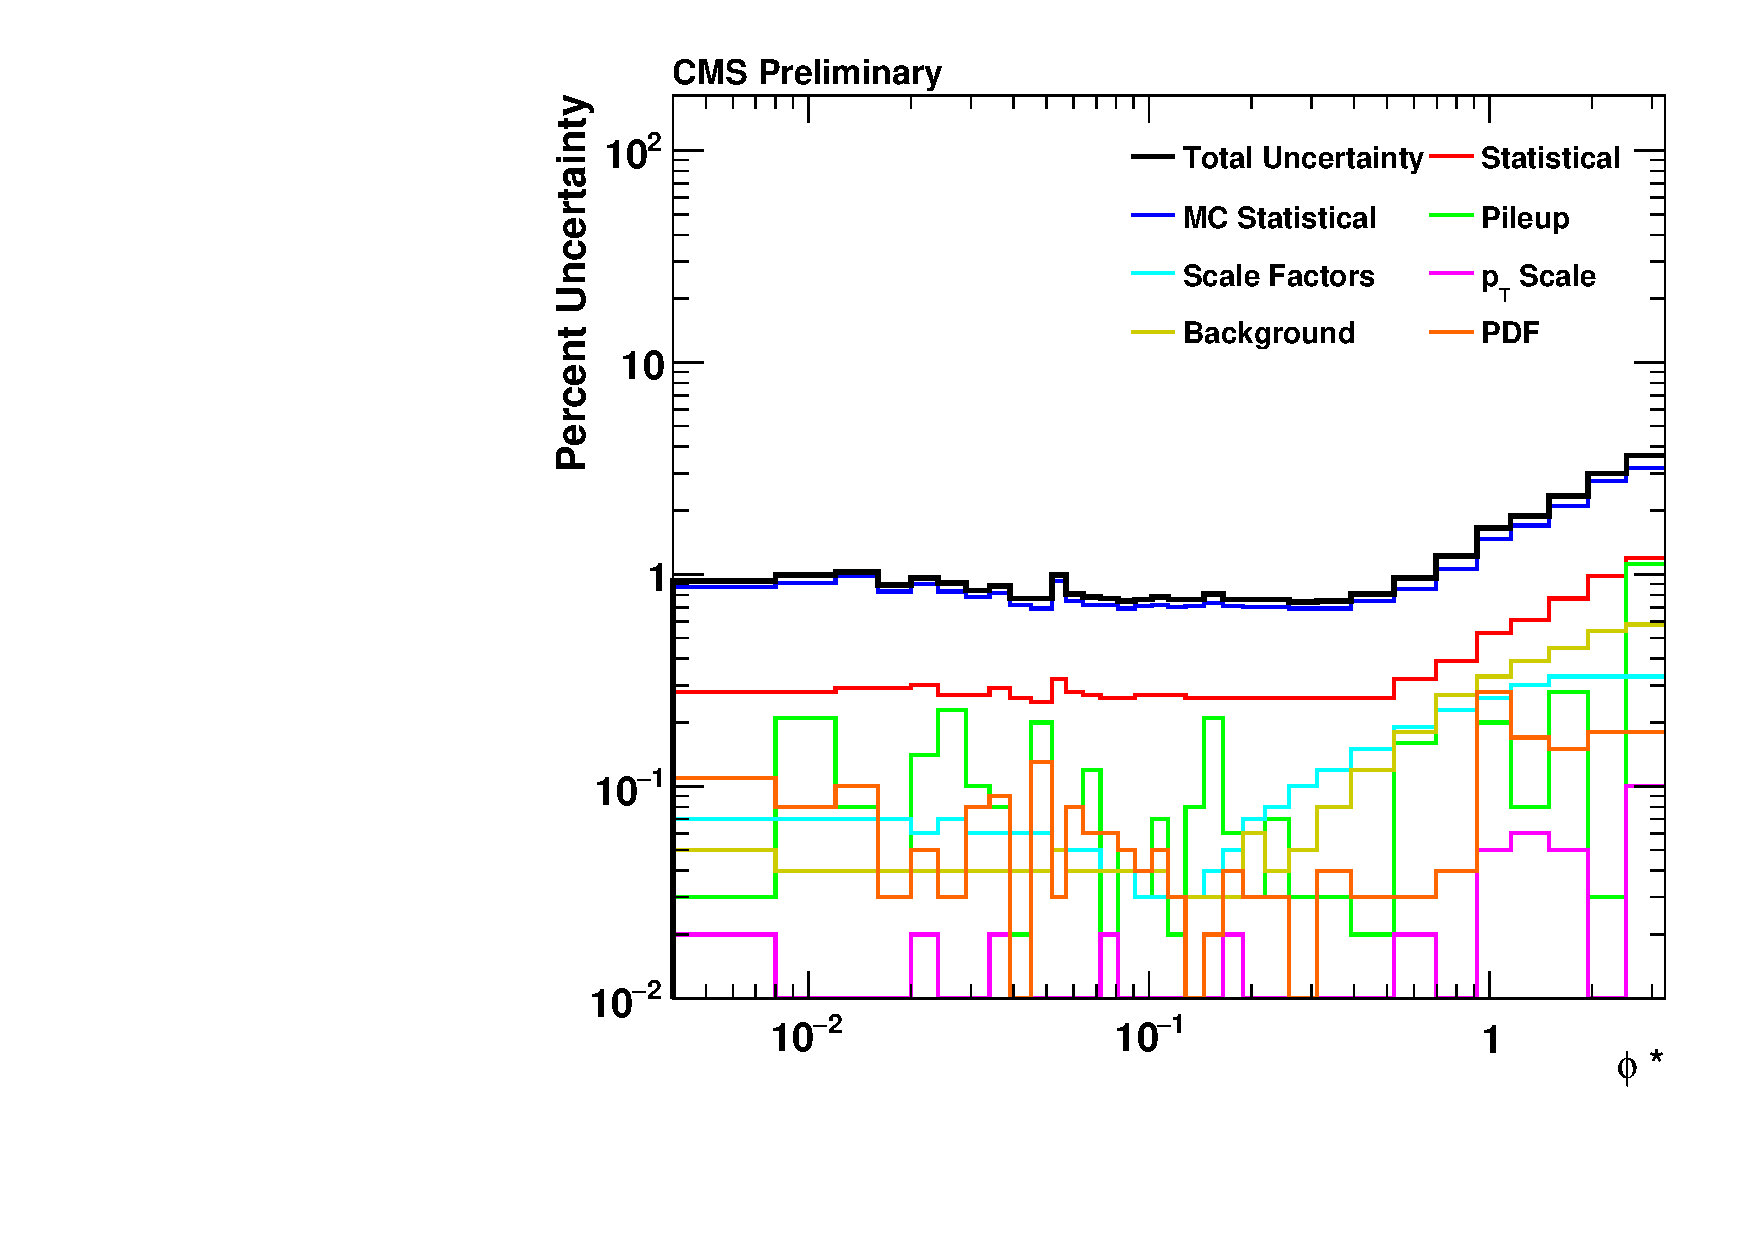
\includegraphics[width=\textwidth]{figures/data_uncertainty_normalized_powheg_unfolded.pdf}
    \caption[
        Fractional errors for the normalized cross section measurement
        made with data unfolded with \POWHEG.
    ]{
        Fractional errors (in \%) for the normalized cross section measurement
        made with data unfolded with \POWHEG. The total value is the sum in
        quadrature of all the other values. These uncertainties are also
        presented in tabular form in \cref{tab:sys_uncert_norm_powheg}.
    }
    \label{fig:sys_uncert_norm_powheg}
\end{figure}


% fig:madgraph_uncert_norm
\begin{figure}[!p]
    \centering
    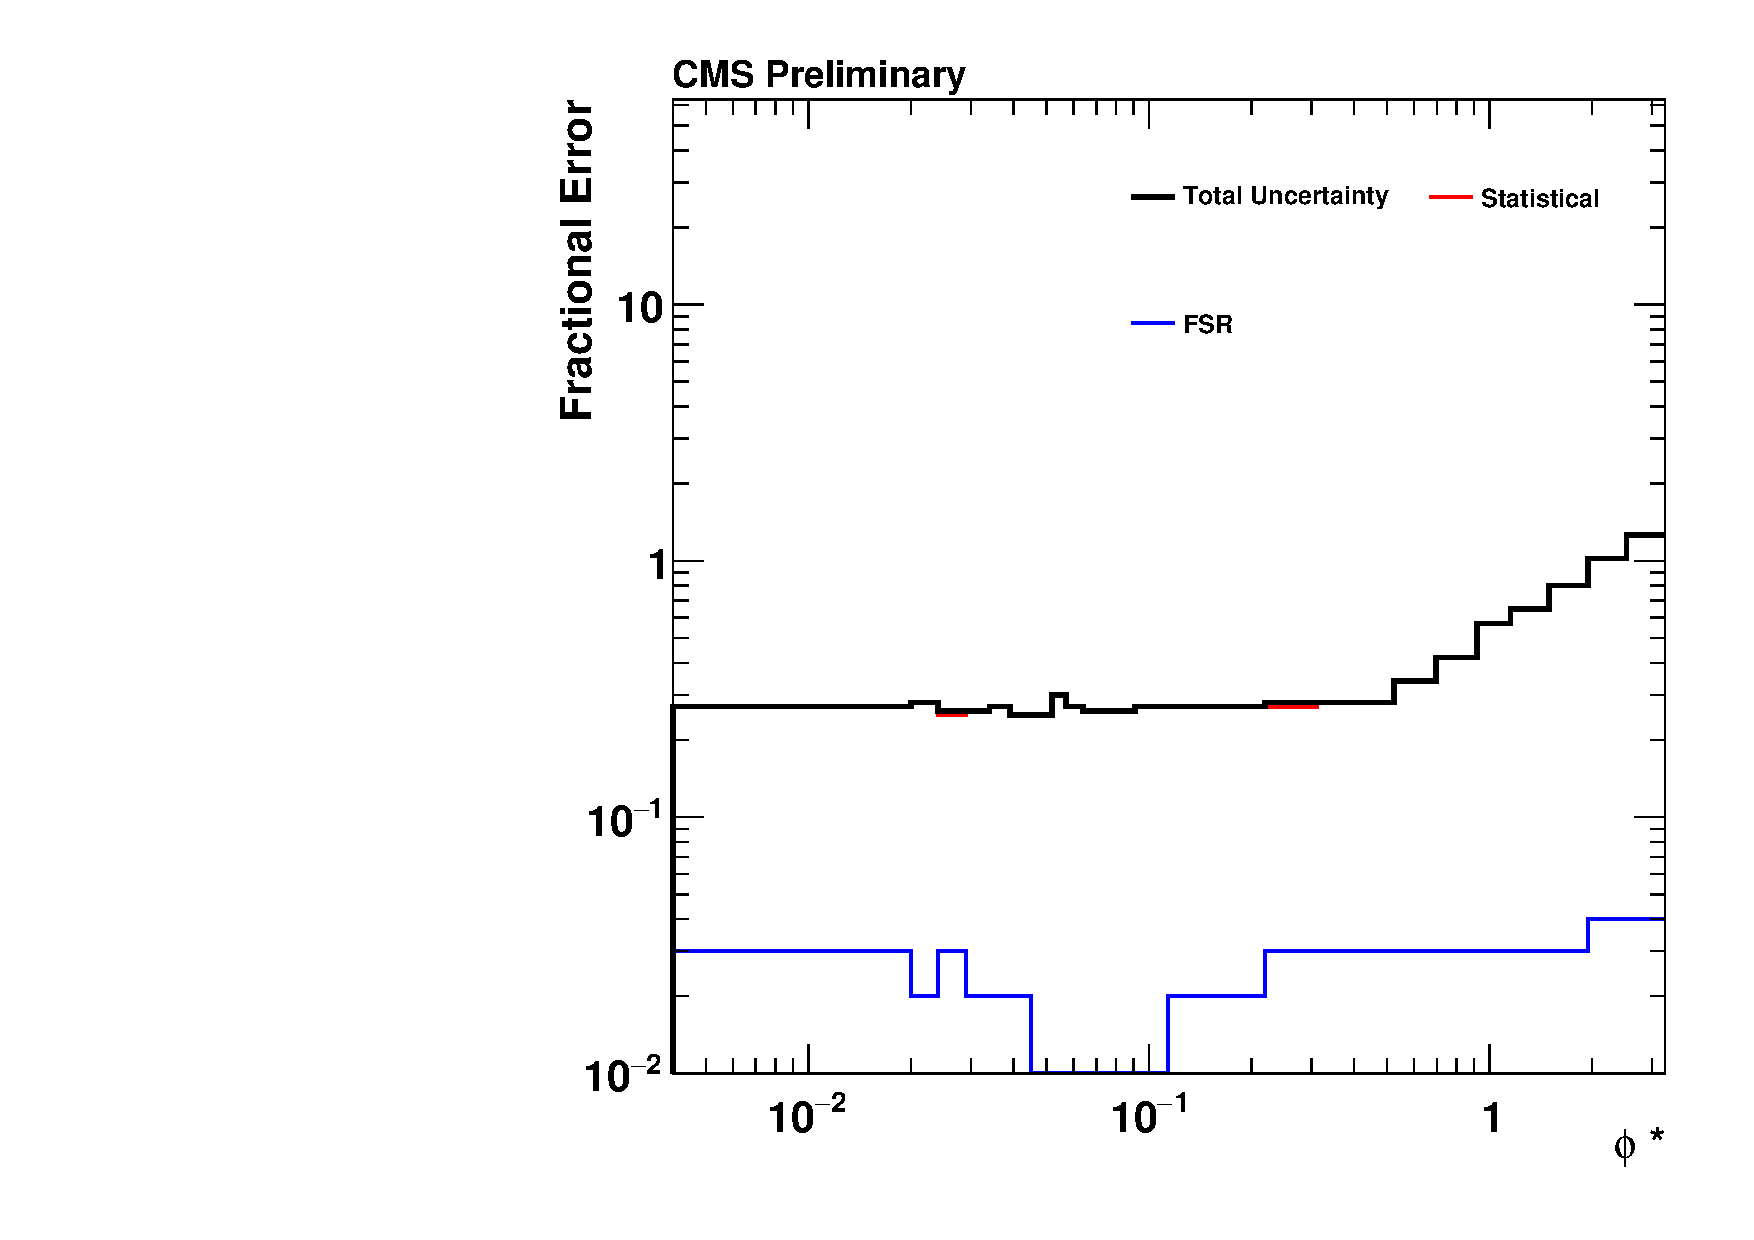
\includegraphics[width=\textwidth]{figures/madgraph_uncertainty_normalized.pdf}
    \caption[
        The uncertainties for the normalized cross section from the \MADGRAPH
        MC sample.
    ]{
        The uncertainties (in \%) for the normalized cross section from the
        \MADGRAPH MC sample. These uncertainties are also presented in tabular
        form in \cref{tab:madgraph_uncert_norm}.
    }
    \label{fig:madgraph_uncert_norm}
\end{figure}


% fig:powheg_uncert_norm
\begin{figure}[!p]
    \centering
    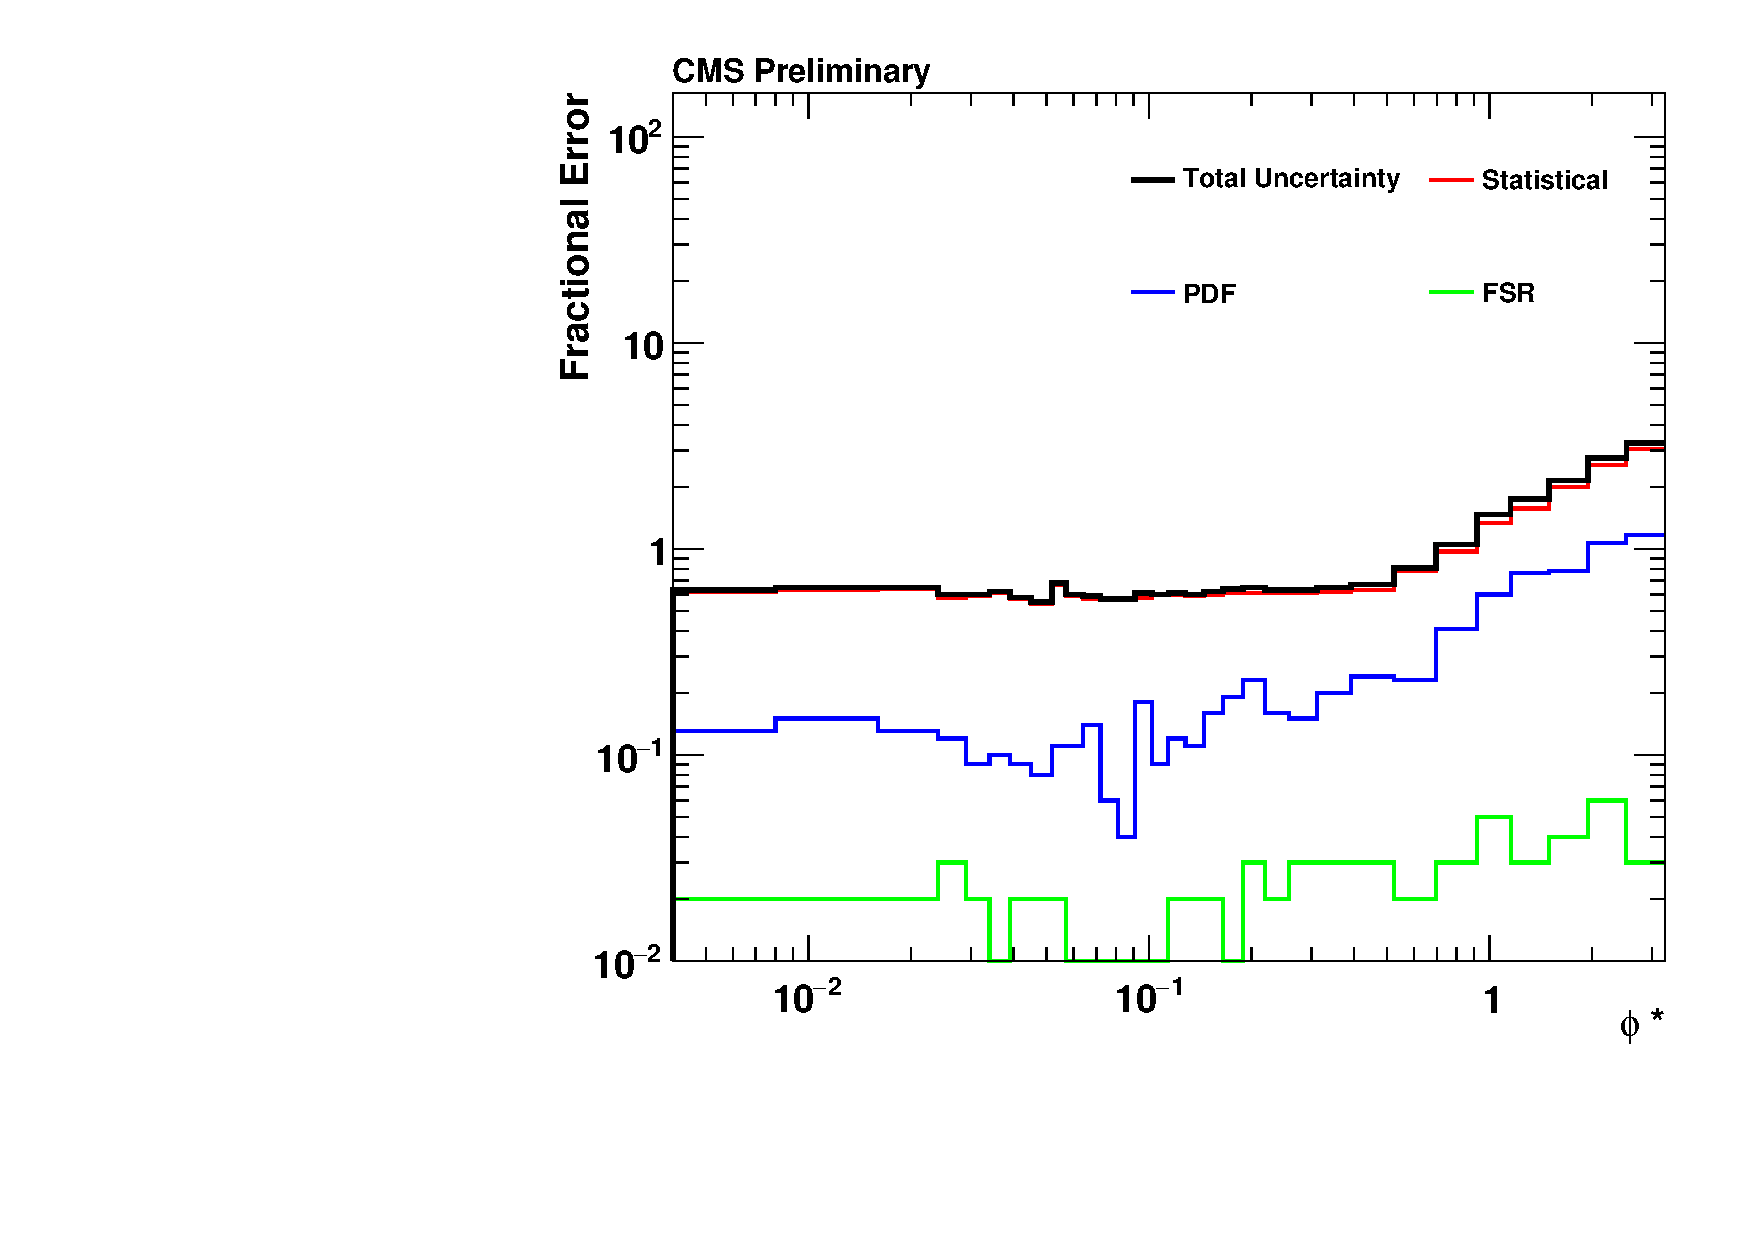
\includegraphics[width=\textwidth]{figures/powheg_uncertainty_normalized.pdf}
    \caption[
        Fractional errors for the normalized cross section from the
        \POWHEG MC sample.
    ]{
        Fractional errors (in \%) for the normalized cross section from the
        \POWHEG MC sample. These uncertainties are also presented in tabular
        form in \cref{tab:powheg_uncert_norm}.
    }
    \label{fig:powheg_uncert_norm}
\end{figure}


\section{Results}
\label{sec:results}

Presented below are our measurements of the differential \phistar cross section
for \Z bosons decaying to an electron pair in the detector region defined in
\SEC~\ref{sec:acceptance}. Two sets of data are used to make the measurement,
one unfolded with \MADGRAPH and one unfolded with \POWHEG; these sets are
otherwise identical. For each set, both an absolute and a normalized cross
section measurement are made. The data distributions of \phistar are compared
to the distributions from both the \MADGRAPH MC signal sample and the \POWHEG
MC signal sample.

\subsection{Absolute Differential Cross Section}
\label{ssec:results_abs}

The absolute differential cross section measurement using data unfolded with
\MADGRAPH is shown in \FIG~\ref{fig:results_abs} and given in tabular form in
\TAB~\ref{tab:results_abs}. The lower plot in \FIG~\ref{fig:results_abs} is
shown in more detail in \FIG~\ref{fig:results_ratio_abs}. As previously
discussed, the primary uncertainty on the data distribution is from the on the
integrated luminosity. The primary uncertainty for the \MADGRAPH sample is the
\FEWZ calculated overall cross section used to scale the distribution, while
the primary uncertainty for the \POWHEG sample is the uncertainty calculated by
varying the \CTten PDF weights.

% fig:results_abs and fig:results_ratio_abs
\begin{figure}[!p]
    \centering
    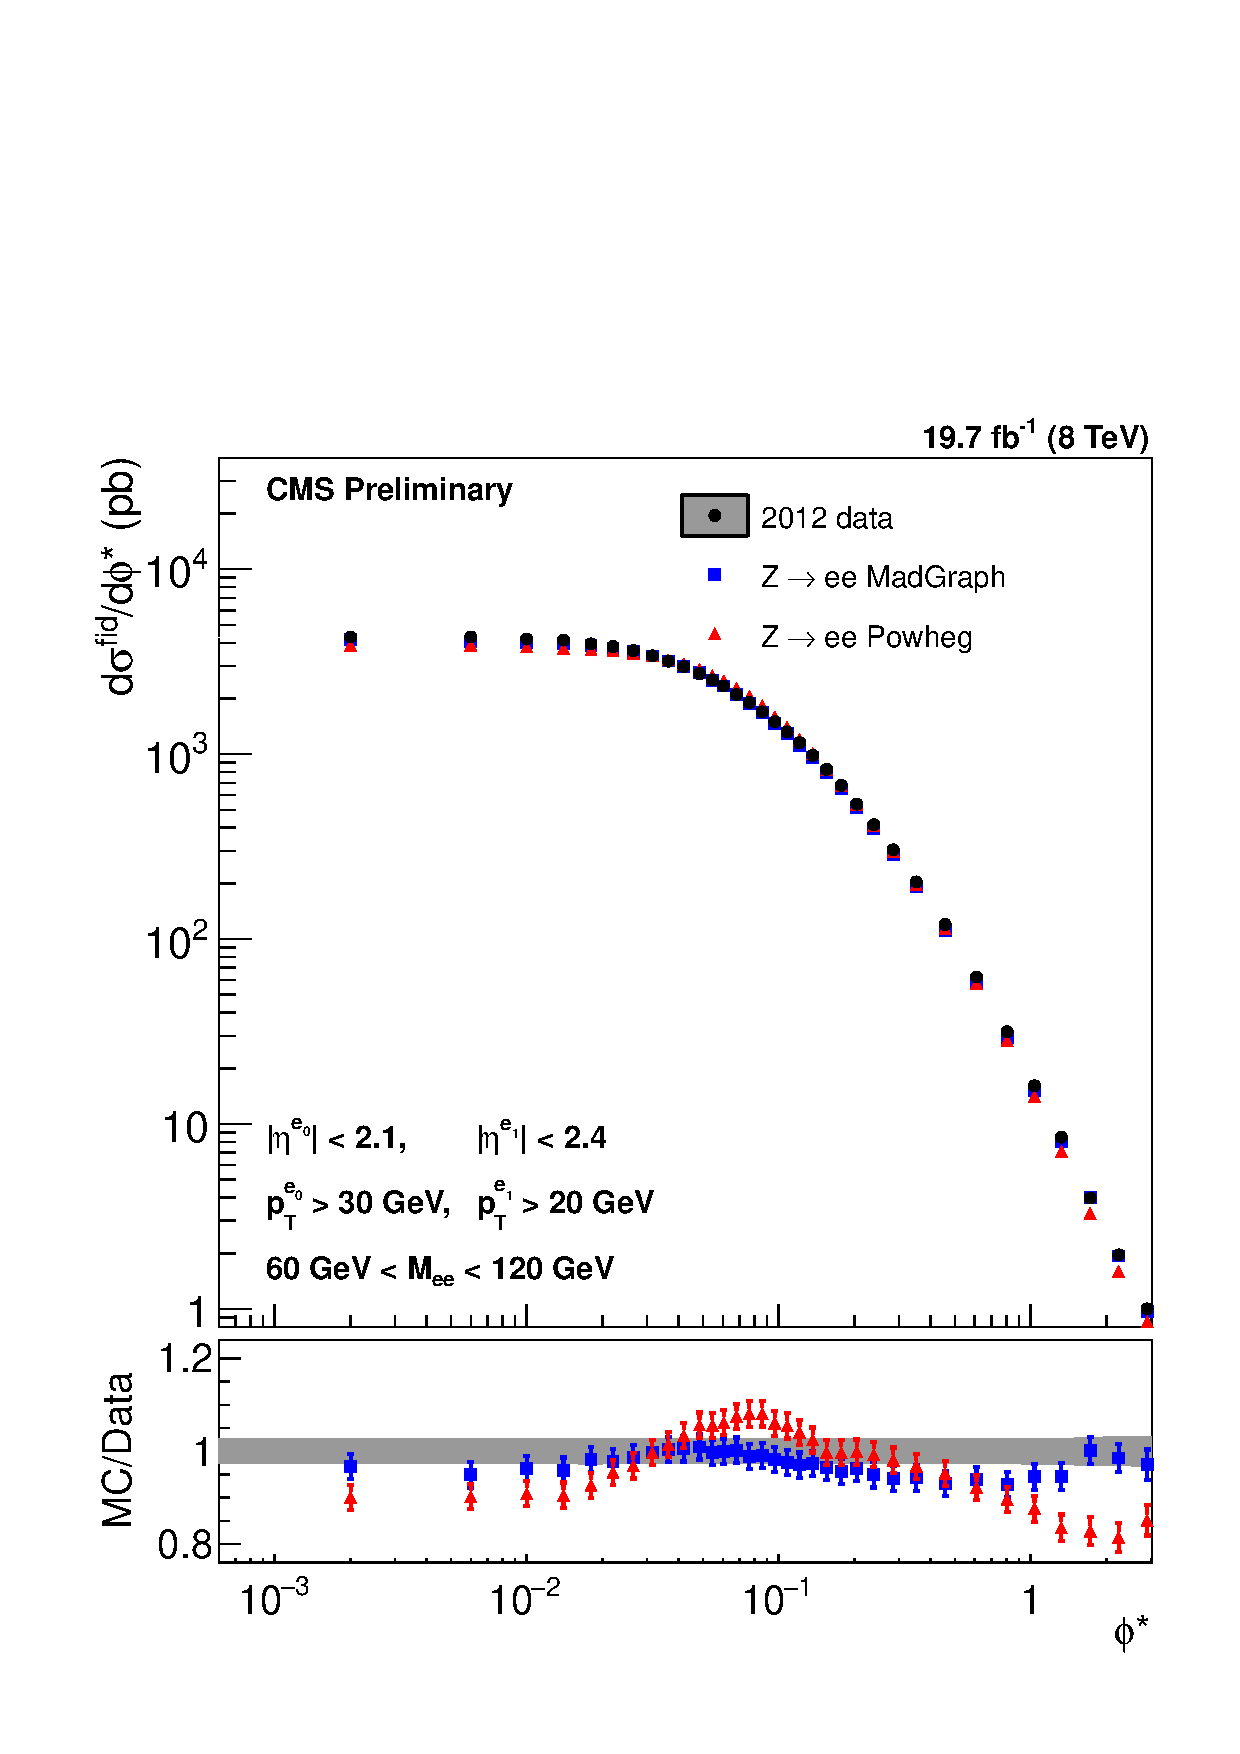
\includegraphics[width=\textwidth]{figures/ZShape_elec_Abs_Dressed.pdf}
    \caption[
        The absolute differential cross section with respects to \phistar for
        \Ztoee events in our fiducial region from data unfolded with \MADGRAPH,
        and the same distributions in \MADGRAPH and \POWHEG.
    ]{
        The absolute differential cross section with respects to \phistar for
        \Ztoee events in our fiducial region from data unfolded with \MADGRAPH,
        and the same distributions in \MADGRAPH and \POWHEG. A close up of the
        lower plot is shown in \cref{fig:results_ratio_abs}.
    }
    \label{fig:results_abs}
\end{figure}

\begin{figure}[!p]
    \centering
    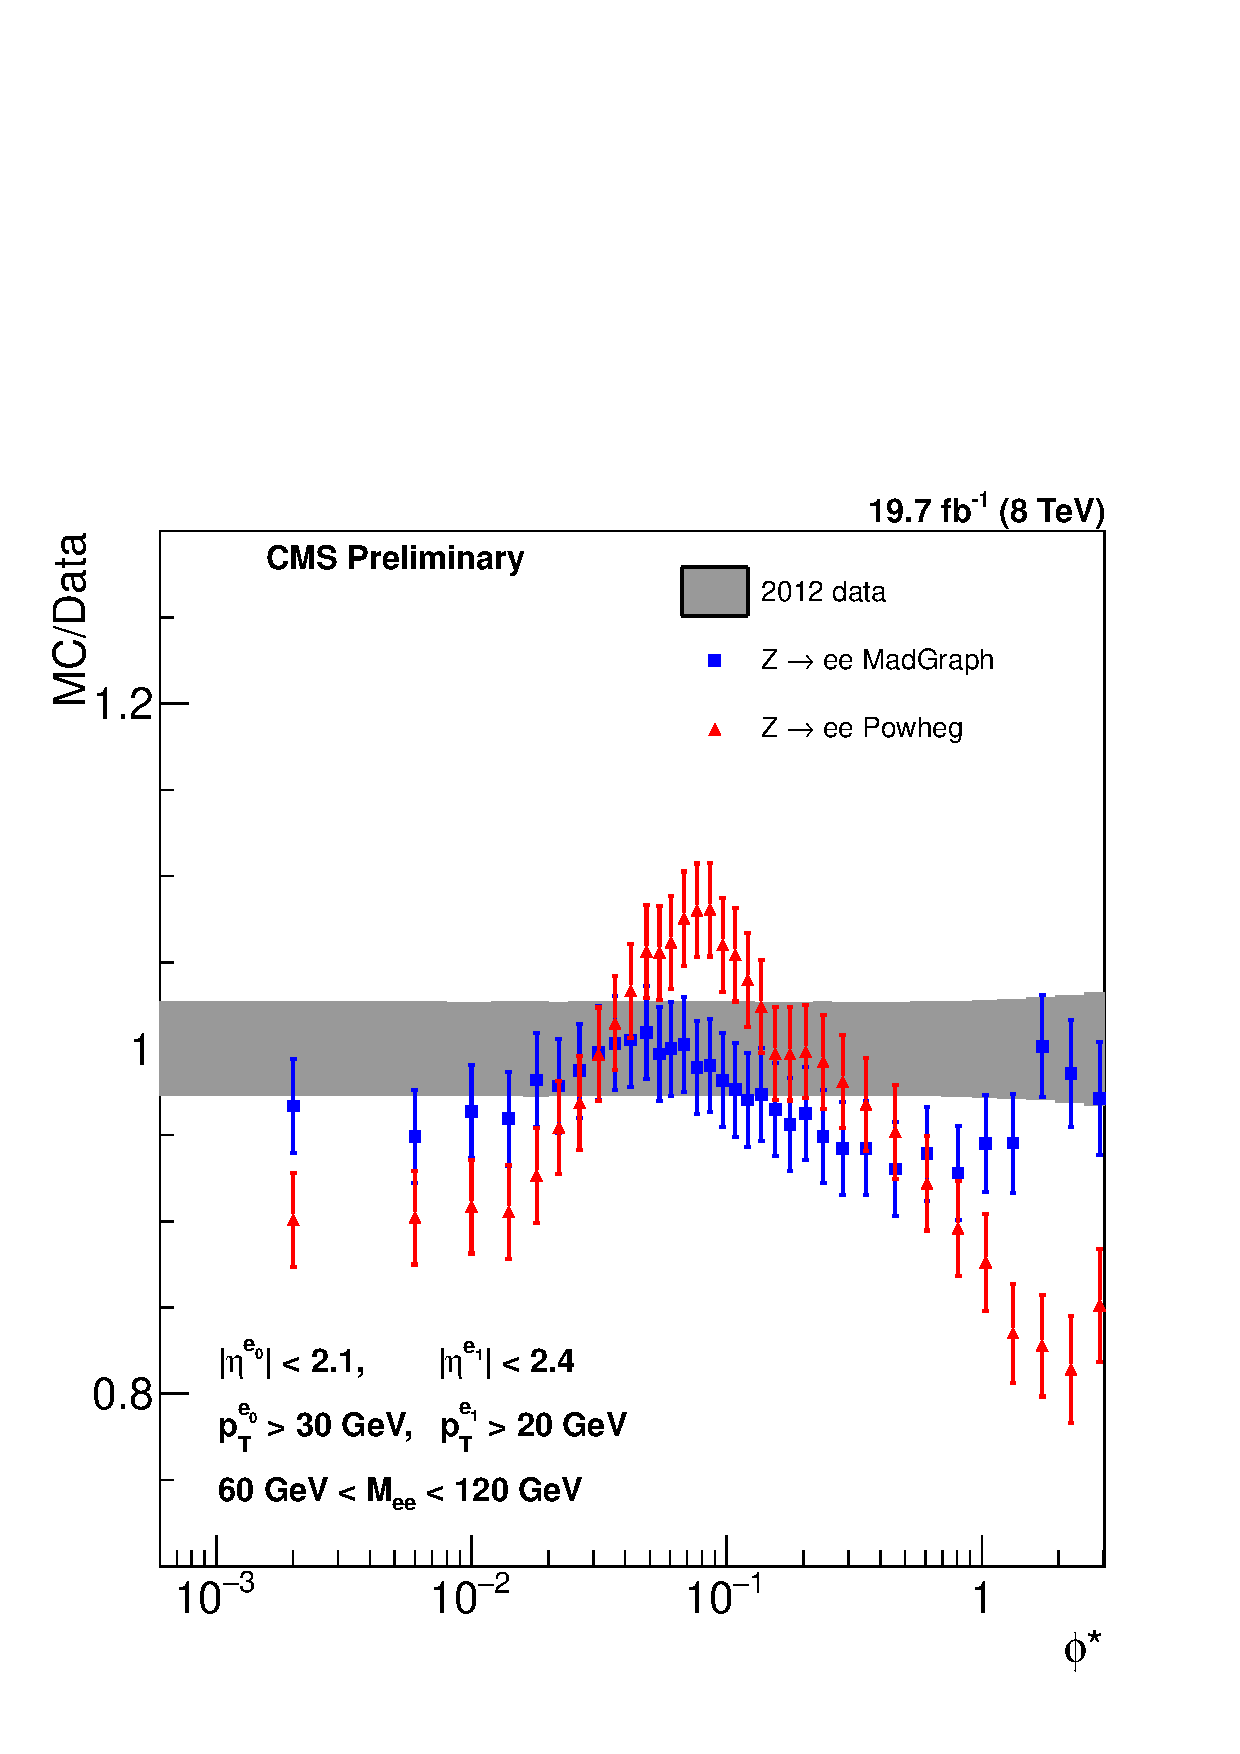
\includegraphics[width=\textwidth]{figures/ZShape_Ratioelec_Abs_Dressed.pdf}
    \caption[
        Close up of the ratio plot from \cref{fig:results_abs} for the
        absolute cross section measurement unfolded with \MADGRAPH.
    ]{
        Close up of the ratio plot from \cref{fig:results_abs} for the
        absolute cross section measurement unfolded with \MADGRAPH. The error
        band indicates the uncertainty in the data, while the square points
        show the ratio of \MADGRAPH over data, and the triangle points show the
        ratio of \POWHEG over data.
    }
    \label{fig:results_ratio_abs}
\end{figure}

% tab:results_abs
\begin{table}
    \spacerows{1.05}
    \begin{center}
        \begin{tabular}{@{}l r r r@{}}
            \toprule
            \phistar range & Data $(\pb)$ & \MADGRAPH $(\pb)$ & \POWHEG $(\pm)$ \\
            \midrule
            0.000--0.004  &  $4297  \pm  117$   &  $4155  \pm  138$   &  $3871  \pm  105$   \\
            0.004--0.008  &  $4302  \pm  117$   &  $4083  \pm  136$   &  $3881  \pm  105$   \\
            0.008--0.012  &  $4190  \pm  113$   &  $4037  \pm  134$   &  $3806  \pm  102$   \\
            0.012--0.016  &  $4137  \pm  113$   &  $3969  \pm  132$   &  $3746  \pm  103$   \\
            0.016--0.020  &  $3951  \pm  109$   &  $3879  \pm  129$   &  $3660  \pm  99$    \\
            0.020--0.024  &  $3816  \pm  103$   &  $3734  \pm  124$   &  $3642  \pm  100$   \\
            0.024--0.029  &  $3632  \pm  99$    &  $3586  \pm  119$   &  $3518  \pm  96$    \\
            0.029--0.034  &  $3404  \pm  93$    &  $3396  \pm  113$   &  $3393  \pm  92$    \\
            0.034--0.039  &  $3182  \pm  87$    &  $3192  \pm  106$   &  $3229  \pm  88$    \\
            0.039--0.045  &  $2971  \pm  81$    &  $2987  \pm  99$    &  $3071  \pm  83$    \\
            0.045--0.052  &  $2724  \pm  74$    &  $2750  \pm  91$    &  $2878  \pm  78$    \\
            0.052--0.057  &  $2521  \pm  69$    &  $2514  \pm  84$    &  $2662  \pm  73$    \\
            0.057--0.064  &  $2335  \pm  63$    &  $2335  \pm  78$    &  $2479  \pm  68$    \\
            0.064--0.072  &  $2099  \pm  57$    &  $2104  \pm  70$    &  $2257  \pm  62$    \\
            0.072--0.081  &  $1904  \pm  52$    &  $1883  \pm  63$    &  $2057  \pm  56$    \\
            0.081--0.091  &  $1694  \pm  46$    &  $1678  \pm  56$    &  $1831  \pm  49$    \\
            0.091--0.102  &  $1498  \pm  41$    &  $1471  \pm  49$    &  $1589  \pm  44$    \\
            0.102--0.114  &  $1320  \pm  36$    &  $1288  \pm  43$    &  $1392  \pm  38$    \\
            0.114--0.128  &  $1152  \pm  31$    &  $1118  \pm  37$    &  $1198  \pm  33$    \\
            0.128--0.145  &  $984   \pm  27$    &  $958   \pm  32$    &  $1008  \pm  27$    \\
            0.145--0.165  &  $827   \pm  22$    &  $797   \pm  27$    &  $824   \pm  22$    \\
            0.165--0.189  &  $678   \pm  18$    &  $648   \pm  22$    &  $676   \pm  18$    \\
            0.189--0.219  &  $537   \pm  15$    &  $517   \pm  17$    &  $536   \pm  15$    \\
            0.219--0.258  &  $415   \pm  11$    &  $394   \pm  13$    &  $412   \pm  11$    \\
            0.258--0.312  &  $304   \pm  8$     &  $287   \pm  10$    &  $298   \pm  8$     \\
            0.312--0.391  &  $204   \pm  6$     &  $192   \pm  6$     &  $197   \pm  5$     \\
            0.391--0.524  &  $120   \pm  3$     &  $112   \pm  4$     &  $114   \pm  3$     \\
            0.524--0.695  &  $62    \pm  2$     &  $59    \pm  2$     &  $58    \pm  2$     \\
            0.695--0.918  &  $31.6  \pm  0.9$   &  $29.3  \pm  1.0$   &  $28.3  \pm  0.7$   \\
            0.918--1.153  &  $16.1  \pm  0.5$   &  $15.2  \pm  0.5$   &  $14.1  \pm  0.4$   \\
            1.153--1.496  &  $8.5   \pm  0.2$   &  $8.0   \pm  0.3$   &  $7.1   \pm  0.2$   \\
            1.496--1.947  &  $4.0   \pm  0.1$   &  $4.0   \pm  0.1$   &  $3.3   \pm  0.1$   \\
            1.947--2.522  &  $1.96  \pm  0.06$  &  $1.93  \pm  0.07$  &  $1.60  \pm  0.06$  \\
            2.522--3.277  &  $1.00  \pm  0.03$  &  $0.97  \pm  0.03$  &  $0.85  \pm  0.03$  \\
            \bottomrule
        \end{tabular}
    \end{center}
    \caption[
        Differential cross-section in \pb with respect to \phistar of \Ztoee.
    ]{
        Differential cross-section in \pb with respect to \phistar of \Ztoee in
        our fiducial region in data and as generated by \MADGRAPH and \POWHEG.
        These results are shown graphically in figure~\ref{fig:result_abs}.
    }
    \label{tab:results_abs}
\end{table}


The absolute differential cross section measurement using data unfolded with
\POWHEG is shown in \FIG~\ref{fig:results_abs_powheg} and given in tabular form
in \TAB~\ref{tab:results_abs_powheg}. The lower plot in
\FIG~\ref{fig:results_abs_powheg} is shown in more detail in
\FIG~\ref{fig:results_ratio_abs_powheg}. The primary uncertainty on the data
distribution is still from the on the integrated luminosity, although the MC
statistical uncertainty is larger in the highest \phistar bins.

% fig:results_abs_powheg and fig:results_ratio_abs_powheg
\begin{figure}[!p]
    \centering
    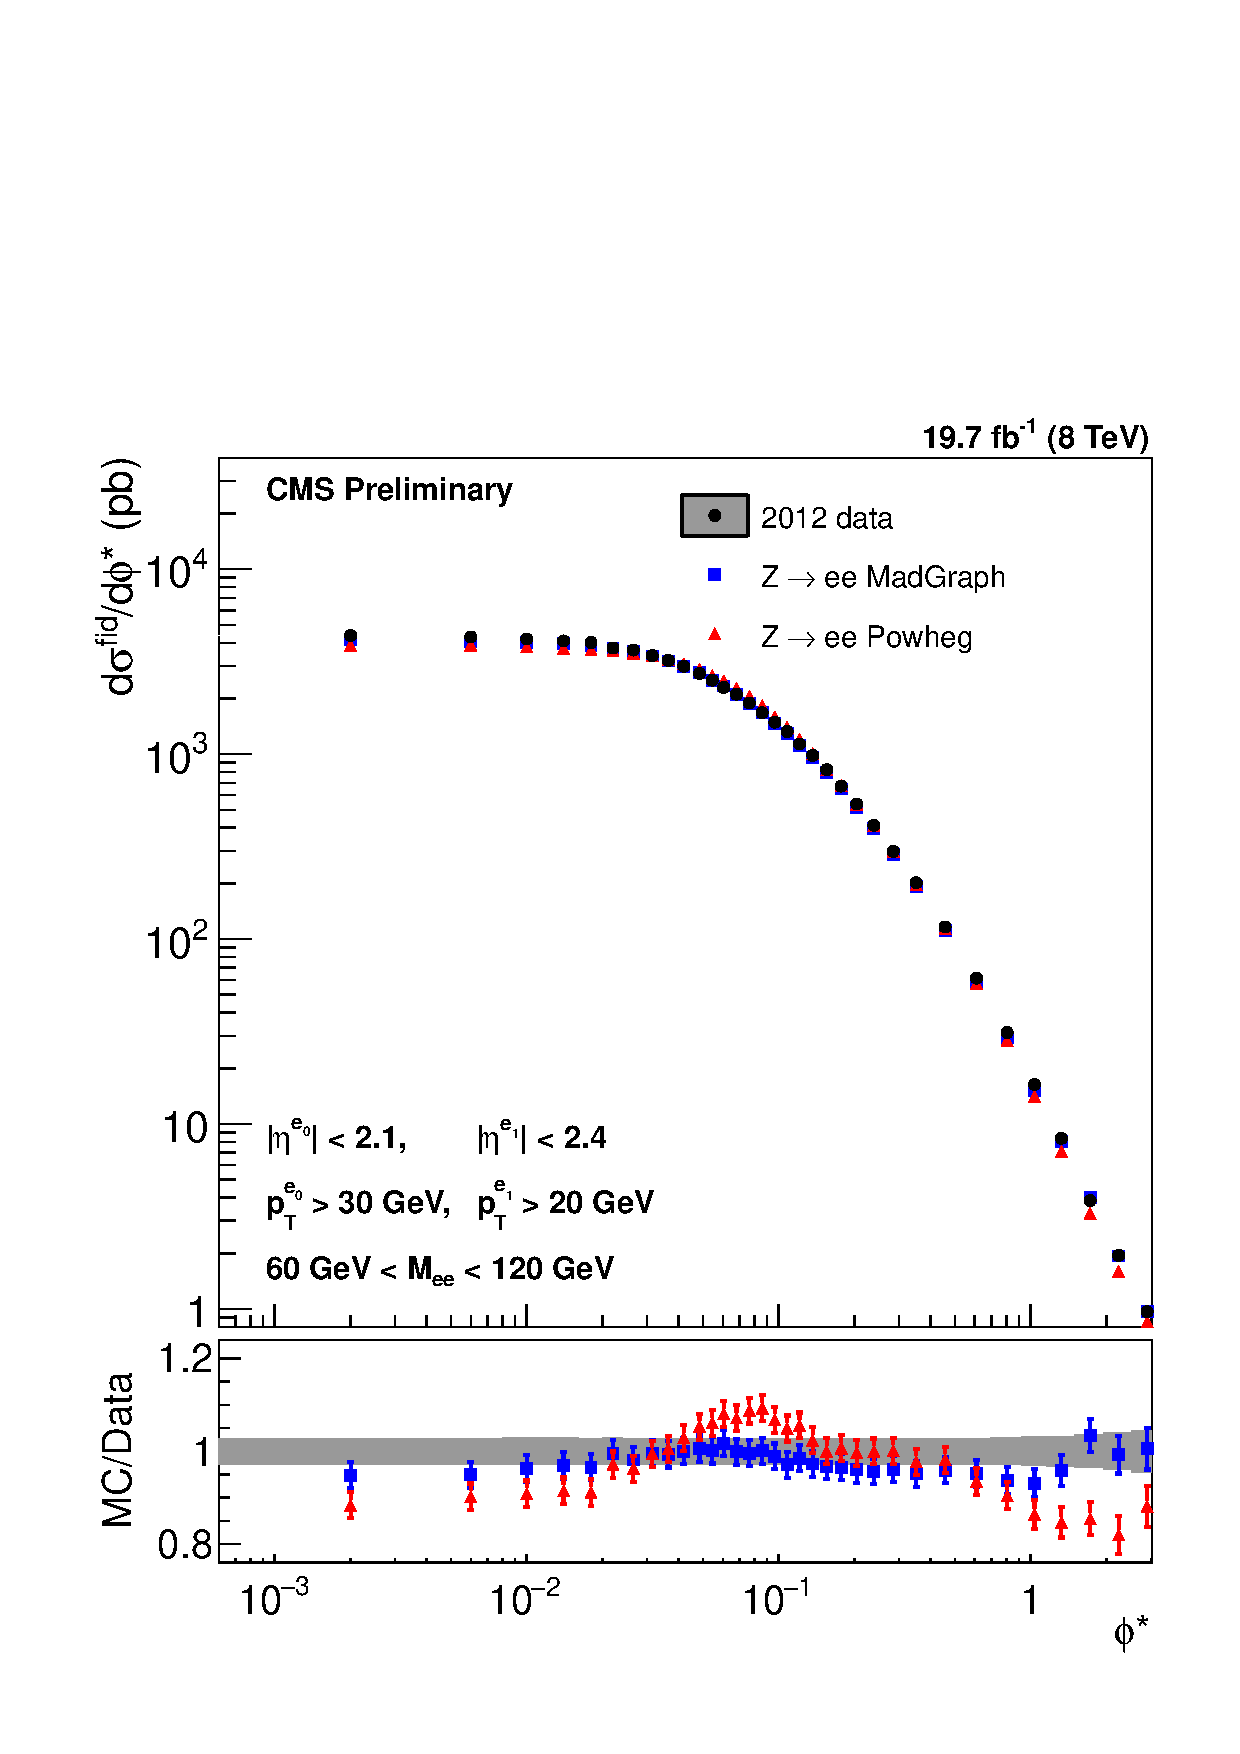
\includegraphics[width=\textwidth]{figures/ZShape_elec_PH_Abs_Dressed.pdf}
    \caption[
        The absolute differential cross section with respects to \phistar for
        \Ztoee events in our fiducial region from data unfolded with
        \PPsixZtwo.
    ]{
        The absolute differential cross section with respects to \phistar for
        \Ztoee events in our fiducial region from data unfolded with
        \PPsixZtwo, and the same distributions in \MADGRAPH and \PPsixZtwo. A
        close up of the lower plot is shown in
        \cref{fig:results_ratio_abs_powheg}.
    }
    \label{fig:results_abs_powheg}
\end{figure}

\begin{figure}[!p]
    \centering
    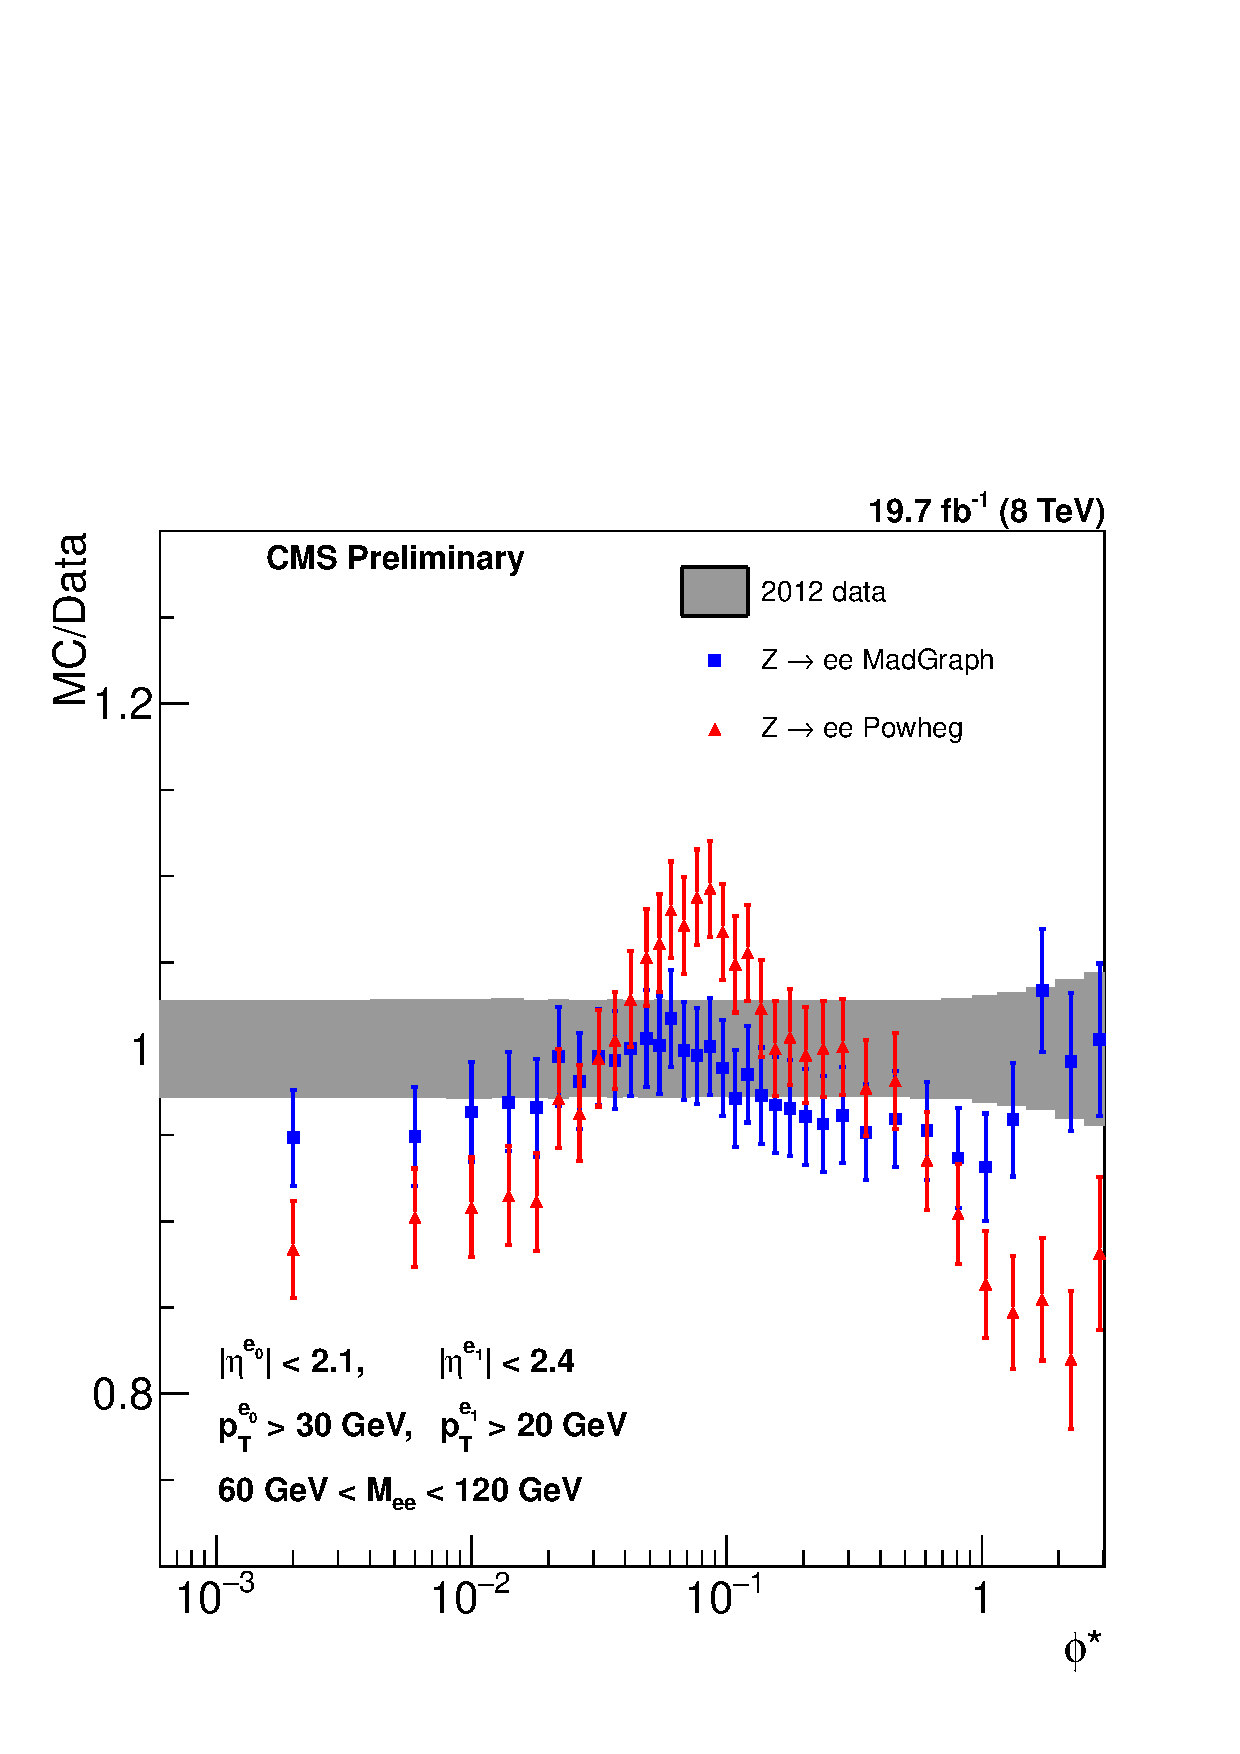
\includegraphics[width=\textwidth]{figures/ZShape_Ratioelec_PH_Abs_Dressed.pdf}
    \caption[
        Close up of the ratio plot from \cref{fig:results_abs_powheg} for the
        absolute cross section measurement unfolded with \PPsixZtwo.
    ]{
        Close up of the ratio plot from \cref{fig:results_abs_powheg} for the
        absolute cross section measurement unfolded with \PPsixZtwo. The error
        band indicates the uncertainty in the data, while the square points
        show the ratio of \MADGRAPH over data, and the triangle points show the
        ratio of \PPsixZtwo over data.
    }
    \label{fig:results_ratio_abs_powheg}
\end{figure}

% tab:results_abs_powheg
\begin{table}
    \spacerows{1.05}
    \begin{center}
        \begin{tabular}{@{}l r r r@{}}
            \toprule
            \phistar range & Data $(\pb)$ & \MADGRAPH $(\pb)$ & \POWHEG $(\pm)$ \\
            \midrule
            0.000--0.004  &  $4381  \pm  122$   &  $4155  \pm  138$   &  $3871  \pm  105$   \\
            0.004--0.008  &  $4302  \pm  122$   &  $4083  \pm  136$   &  $3881  \pm  105$   \\
            0.008--0.012  &  $4191  \pm  121$   &  $4037  \pm  134$   &  $3806  \pm  102$   \\
            0.012--0.016  &  $4096  \pm  118$   &  $3969  \pm  132$   &  $3746  \pm  103$   \\
            0.016--0.020  &  $4016  \pm  113$   &  $3879  \pm  129$   &  $3660  \pm  99$    \\
            0.020--0.024  &  $3751  \pm  108$   &  $3734  \pm  124$   &  $3642  \pm  100$   \\
            0.024--0.029  &  $3654  \pm  102$   &  $3586  \pm  119$   &  $3518  \pm  96$    \\
            0.029--0.034  &  $3412  \pm  95$    &  $3396  \pm  113$   &  $3393  \pm  92$    \\
            0.034--0.039  &  $3213  \pm  91$    &  $3192  \pm  106$   &  $3229  \pm  88$    \\
            0.039--0.045  &  $2985  \pm  83$    &  $2987  \pm  99$    &  $3071  \pm  83$    \\
            0.045--0.052  &  $2734  \pm  77$    &  $2750  \pm  91$    &  $2878  \pm  78$    \\
            0.052--0.057  &  $2509  \pm  71$    &  $2514  \pm  84$    &  $2662  \pm  73$    \\
            0.057--0.064  &  $2295  \pm  65$    &  $2335  \pm  78$    &  $2479  \pm  68$    \\
            0.064--0.072  &  $2107  \pm  59$    &  $2104  \pm  70$    &  $2257  \pm  62$    \\
            0.072--0.081  &  $1891  \pm  53$    &  $1883  \pm  63$    &  $2057  \pm  56$    \\
            0.081--0.091  &  $1676  \pm  47$    &  $1678  \pm  56$    &  $1831  \pm  49$    \\
            0.091--0.102  &  $1488  \pm  41$    &  $1471  \pm  49$    &  $1589  \pm  44$    \\
            0.102--0.114  &  $1327  \pm  37$    &  $1288  \pm  43$    &  $1392  \pm  38$    \\
            0.114--0.128  &  $1135  \pm  32$    &  $1118  \pm  37$    &  $1198  \pm  33$    \\
            0.128--0.145  &  $985   \pm  28$    &  $958   \pm  32$    &  $1008  \pm  27$    \\
            0.145--0.165  &  $824   \pm  23$    &  $797   \pm  27$    &  $824   \pm  22$    \\
            0.165--0.189  &  $671   \pm  19$    &  $648   \pm  22$    &  $676   \pm  18$    \\
            0.189--0.219  &  $538   \pm  15$    &  $517   \pm  17$    &  $536   \pm  15$    \\
            0.219--0.258  &  $412   \pm  11$    &  $394   \pm  13$    &  $412   \pm  11$    \\
            0.258--0.312  &  $298   \pm  8$     &  $287   \pm  10$    &  $298   \pm  8$     \\
            0.312--0.391  &  $202   \pm  6$     &  $192   \pm  6$     &  $197   \pm  5$     \\
            0.391--0.524  &  $116   \pm  3$     &  $112   \pm  4$     &  $114   \pm  3$     \\
            0.524--0.695  &  $61    \pm  2$     &  $59    \pm  2$     &  $58    \pm  2$     \\
            0.695--0.918  &  $31.3  \pm  0.9$   &  $29.3  \pm  1.0$   &  $28.3  \pm  0.7$   \\
            0.918--1.153  &  $16.4  \pm  0.5$   &  $15.2  \pm  0.5$   &  $14.1  \pm  0.4$   \\
            1.153--1.496  &  $8.4   \pm  0.3$   &  $8.0   \pm  0.3$   &  $7.1   \pm  0.2$   \\
            1.496--1.947  &  $3.9   \pm  0.1$   &  $4.0   \pm  0.1$   &  $3.3   \pm  0.1$   \\
            1.947--2.522  &  $1.95  \pm  0.08$  &  $1.93  \pm  0.07$  &  $1.60  \pm  0.06$  \\
            2.522--3.277  &  $0.97  \pm  0.04$  &  $0.97  \pm  0.03$  &  $0.85  \pm  0.03$  \\
            \bottomrule
        \end{tabular}
    \end{center}
    \caption[
        The absolute differential cross section in \pb with respects to
        \phistar for \Ztoee events in our fiducial region from data unfolded
        with \POWHEG.
    ]{
        The absolute differential cross section in \pb with respects to
        \phistar for \Ztoee events in our fiducial region from data unfolded
        with \POWHEG, and the same distributions in \MADGRAPH and \POWHEG.
        These results are shown graphically in
        figure~\ref{fig:results_abs_powheg}.
    }
    \label{tab:results_abs_powheg}
\end{table}


\subsection{Normalized Differential Cross Section}
\label{ssec:results_norm}

The normalized differential cross section measurement using data unfolded with
\MADGRAPH is shown in \FIG~\ref{fig:results_norm} and given in tabular form in
\TAB~\ref{tab:results_norm}. The lower plot in \FIG~\ref{fig:results_norm} is
shown in more detail in \FIG~\ref{fig:results_ratio_norm}. As the luminosity
has canceled out in the normalization, the primary uncertainty on the data is
now the statistical uncertainty from the \MADGRAPH sample used to unfold the
it. The limit number of events in the MC samples is also the primary
uncertainty on the \MADGRAPH distribution and the \POWHEG distribution.

% fig:results_norm and fig:results_ratio_norm
\begin{figure}[!p]
    \centering
    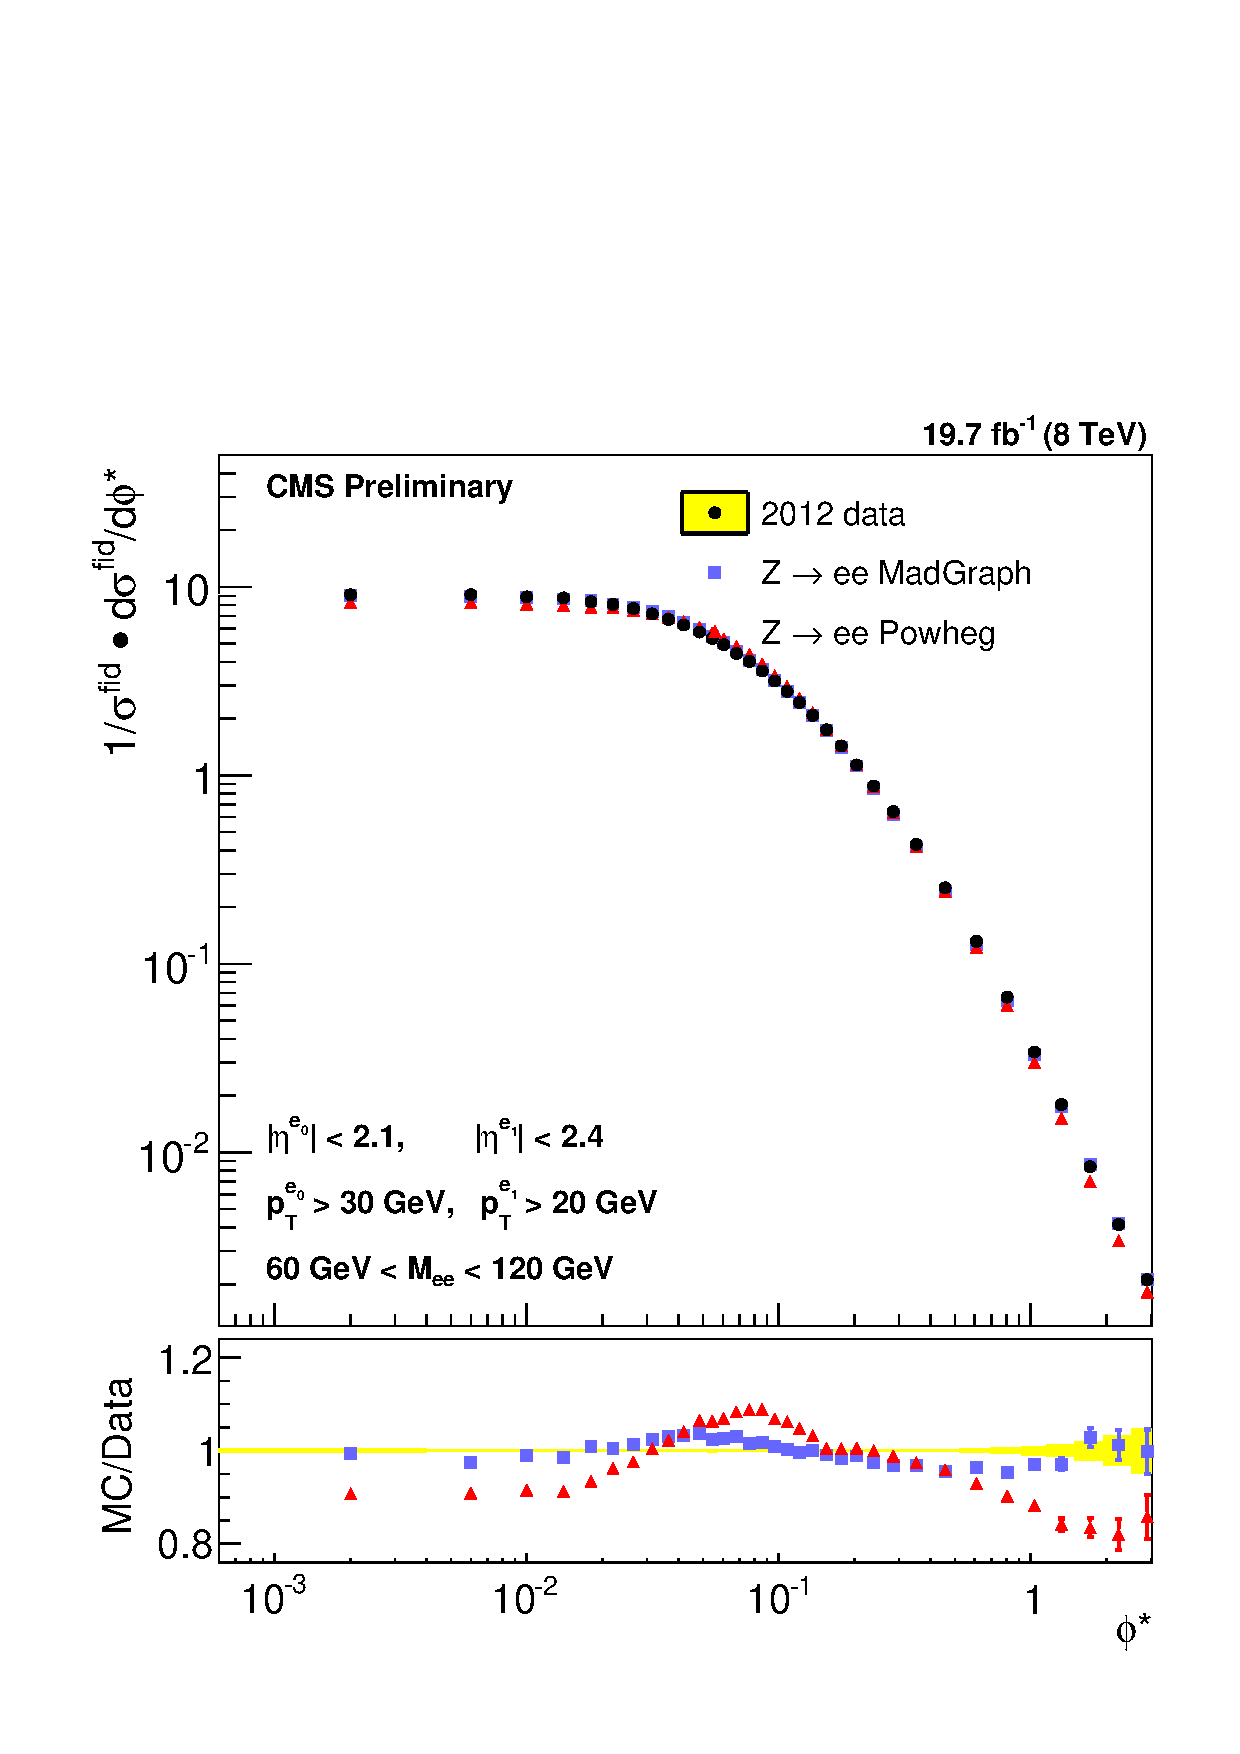
\includegraphics[width=\textwidth]{figures/ZShape_elec_Norm_Dressed.pdf}
    \caption[
        The absolute differential cross section with respects to \phistar for
        \Ztoee events in our fiducial region from data unfolded with \MADGRAPH,
        and the same distributions in \MADGRAPH and \POWHEG.
    ]{
        The absolute differential cross section with respects to \phistar for
        \Ztoee events in our fiducial region from data unfolded with \MADGRAPH,
        and the same distributions in \MADGRAPH and \POWHEG. A close up of the
        lower plot is shown in \FIG~\ref{fig:results_ratio_norm}.
    }
    \label{fig:results_norm}
\end{figure}

\begin{figure}[!p]
    \centering
    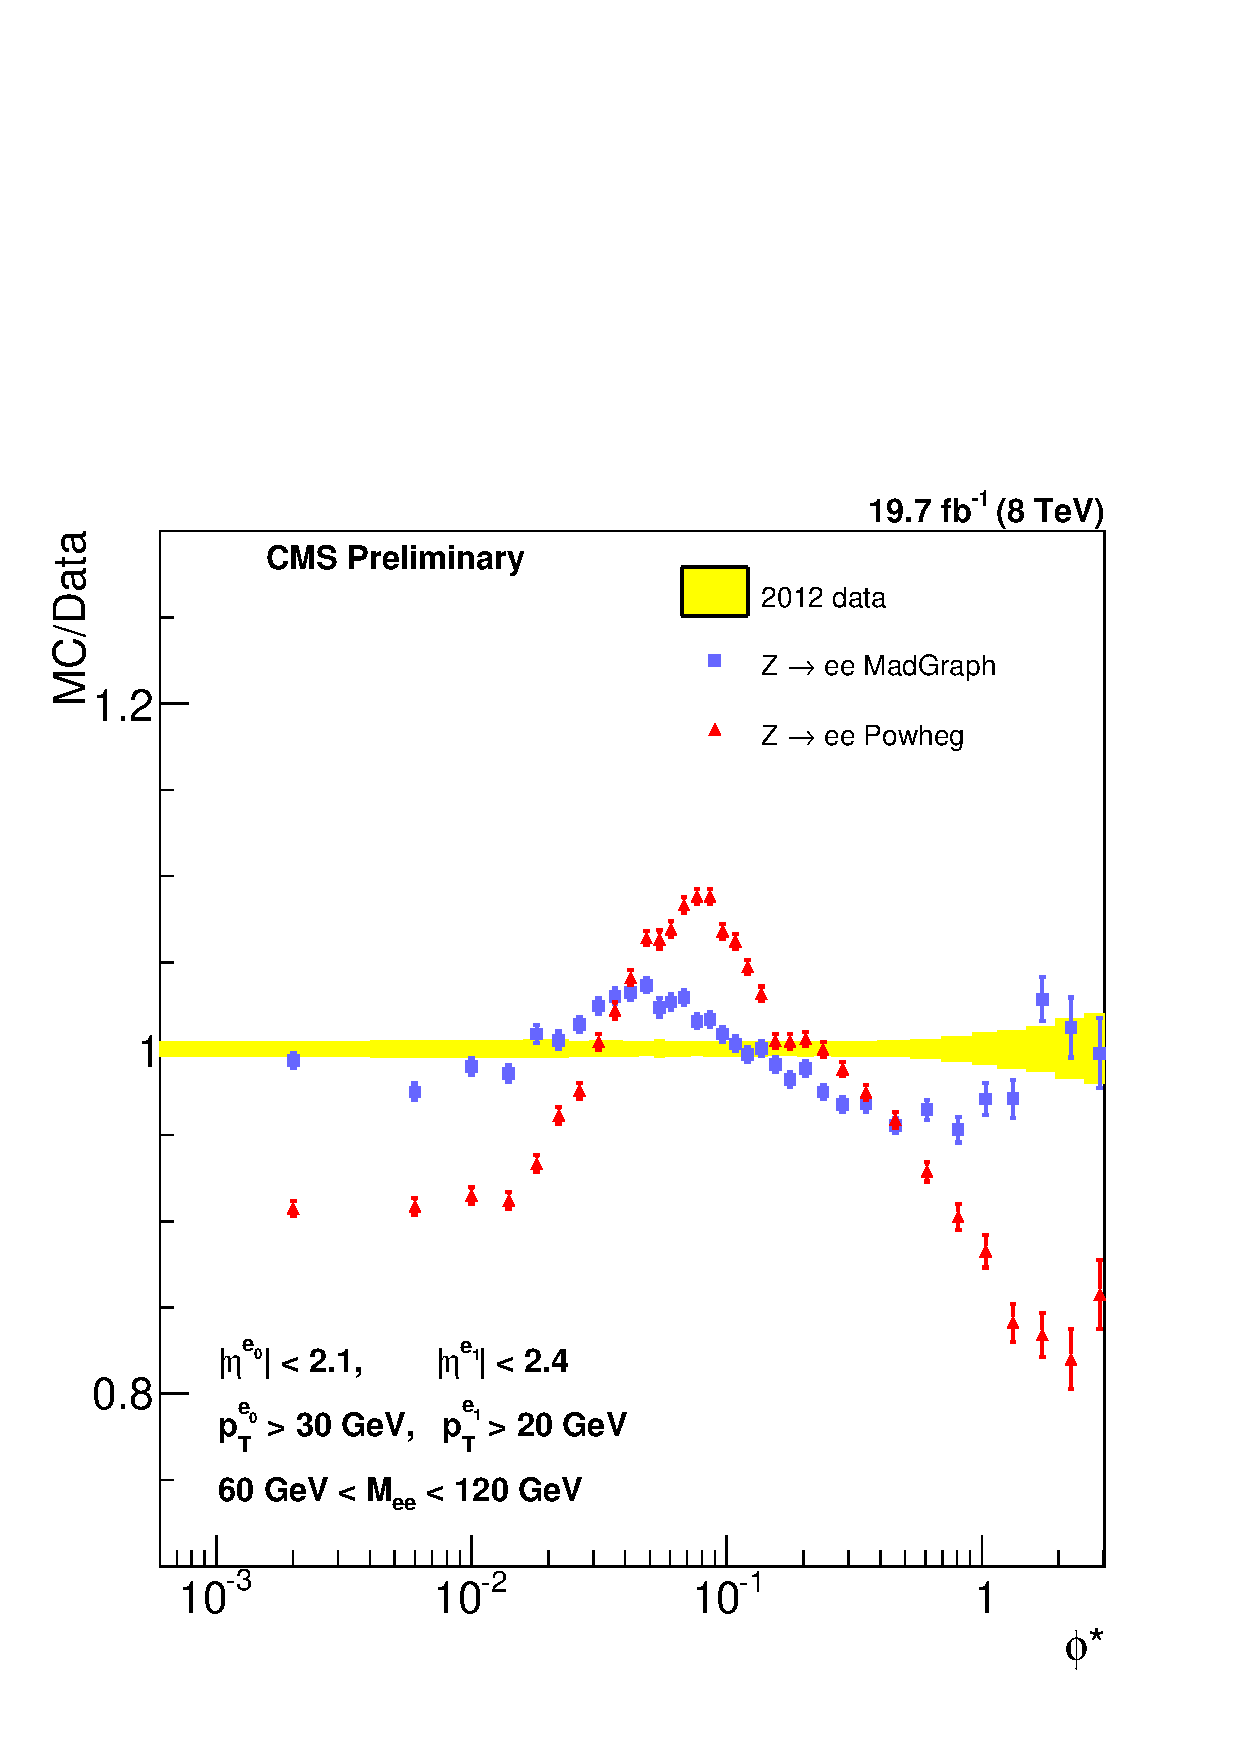
\includegraphics[width=\textwidth]{figures/ZShape_Ratioelec_Norm_Dressed.pdf}
    \caption[
        Close up of the ratio plot from \FIG~\ref{fig:results_norm} for the
        normalized cross section measurement unfolded with \MADGRAPH.
    ]{
        Close up of the ratio plot from \FIG~\ref{fig:results_norm} for the
        normalized cross section measurement unfolded with \MADGRAPH. The error
        band indicates the uncertainty in the data, while the square points
        show the ratio of \MADGRAPH over data, and the triangle points show the
        ratio of \POWHEG over data.
    }
    \label{fig:results_ratio_norm}
\end{figure}

% tab:results_norm
\begin{table}
    \spacerows{1.05}
    \begin{center}
        \begin{tabular}{@{}l r r r@{}}
            \toprule
            \phistar range & Data & \MADGRAPH & \POWHEG \\
            \midrule
            0.000--0.004  &  $9.08     \pm  0.04$     &  $9.01     \pm  0.02$     &  $8.24     \pm  0.05$     \\
            0.004--0.008  &  $9.09     \pm  0.05$     &  $8.86     \pm  0.02$     &  $8.26     \pm  0.05$     \\
            0.008--0.012  &  $8.85     \pm  0.04$     &  $8.76     \pm  0.02$     &  $8.10     \pm  0.05$     \\
            0.012--0.016  &  $8.74     \pm  0.04$     &  $8.61     \pm  0.02$     &  $7.97     \pm  0.05$     \\
            0.016--0.020  &  $8.34     \pm  0.04$     &  $8.42     \pm  0.02$     &  $7.79     \pm  0.05$     \\
            0.020--0.024  &  $8.06     \pm  0.04$     &  $8.10     \pm  0.02$     &  $7.75     \pm  0.05$     \\
            0.024--0.029  &  $7.67     \pm  0.03$     &  $7.78     \pm  0.02$     &  $7.48     \pm  0.04$     \\
            0.029--0.034  &  $7.19     \pm  0.03$     &  $7.37     \pm  0.02$     &  $7.22     \pm  0.04$     \\
            0.034--0.039  &  $6.72     \pm  0.03$     &  $6.93     \pm  0.02$     &  $6.87     \pm  0.04$     \\
            0.039--0.045  &  $6.28     \pm  0.03$     &  $6.48     \pm  0.02$     &  $6.53     \pm  0.04$     \\
            0.045--0.052  &  $5.75     \pm  0.02$     &  $5.97     \pm  0.01$     &  $6.12     \pm  0.03$     \\
            0.052--0.057  &  $5.33     \pm  0.03$     &  $5.45     \pm  0.02$     &  $5.66     \pm  0.04$     \\
            0.057--0.064  &  $4.93     \pm  0.02$     &  $5.07     \pm  0.01$     &  $5.28     \pm  0.03$     \\
            0.064--0.072  &  $4.43     \pm  0.02$     &  $4.57     \pm  0.01$     &  $4.80     \pm  0.03$     \\
            0.072--0.081  &  $4.02     \pm  0.02$     &  $4.09     \pm  0.01$     &  $4.38     \pm  0.02$     \\
            0.081--0.091  &  $3.58     \pm  0.02$     &  $3.640    \pm  0.010$    &  $3.90     \pm  0.02$     \\
            0.091--0.102  &  $3.17     \pm  0.01$     &  $3.192    \pm  0.009$    &  $3.38     \pm  0.02$     \\
            0.102--0.114  &  $2.79     \pm  0.01$     &  $2.795    \pm  0.008$    &  $2.96     \pm  0.02$     \\
            0.114--0.128  &  $2.43     \pm  0.01$     &  $2.426    \pm  0.007$    &  $2.55     \pm  0.02$     \\
            0.128--0.145  &  $2.079    \pm  0.009$    &  $2.079    \pm  0.006$    &  $2.14     \pm  0.01$     \\
            0.145--0.165  &  $1.746    \pm  0.007$    &  $1.730    \pm  0.005$    &  $1.75     \pm  0.01$     \\
            0.165--0.189  &  $1.432    \pm  0.006$    &  $1.406    \pm  0.004$    &  $1.438    \pm  0.009$    \\
            0.189--0.219  &  $1.134    \pm  0.005$    &  $1.121    \pm  0.003$    &  $1.140    \pm  0.007$    \\
            0.219--0.258  &  $0.877    \pm  0.004$    &  $0.855    \pm  0.002$    &  $0.877    \pm  0.006$    \\
            0.258--0.312  &  $0.642    \pm  0.003$    &  $0.622    \pm  0.002$    &  $0.635    \pm  0.004$    \\
            0.312--0.391  &  $0.430    \pm  0.002$    &  $0.417    \pm  0.001$    &  $0.420    \pm  0.003$    \\
            0.391--0.524  &  $0.253    \pm  0.001$    &  $0.2421   \pm  0.0007$   &  $0.243    \pm  0.002$    \\
            0.524--0.695  &  $0.1317   \pm  0.0007$   &  $0.1271   \pm  0.0004$   &  $0.1224   \pm  0.0010$   \\
            0.695--0.918  &  $0.0667   \pm  0.0005$   &  $0.0635   \pm  0.0003$   &  $0.0602   \pm  0.0006$   \\
            0.918--1.153  &  $0.0340   \pm  0.0003$   &  $0.0330   \pm  0.0002$   &  $0.0300   \pm  0.0004$   \\
            1.153--1.496  &  $0.0179   \pm  0.0002$   &  $0.0174   \pm  0.0001$   &  $0.0151   \pm  0.0003$   \\
            1.496--1.947  &  $0.0084   \pm  0.0001$   &  $0.00865  \pm  0.00007$  &  $0.0070   \pm  0.0002$   \\
            1.947--2.522  &  $0.00415  \pm  0.00007$  &  $0.00420  \pm  0.00004$  &  $0.00340  \pm  0.00009$  \\
            2.522--3.277  &  $0.00212  \pm  0.00004$  &  $0.00211  \pm  0.00003$  &  $0.00181  \pm  0.00006$  \\
            \bottomrule
        \end{tabular}
    \end{center}
    \caption[
        Normalized differential cross-section with respect to \phistar of
        \Ztoee.
    ]{
        Normalized differential cross-section with respect to \phistar of
        \Ztoee in our fiducial region in data and as generated by \MADGRAPH and
        \POWHEG. These results are shown graphically in
        figure~\ref{fig:results_norm}.
    }
    \label{tab:results_norm}
\end{table}


The normalized differential cross section measurement using data unfolded with
\POWHEG is shown in \FIG~\ref{fig:results_norm_powheg} and given in tabular
form in \TAB~\ref{tab:results_norm_powheg}. The lower plot in
\FIG~\ref{fig:results_norm_powheg} is shown in more detail in
\FIG~\ref{fig:results_ratio_norm_powheg}. The primary uncertainty on the data
is now the statistical uncertainty from the \POWHEG sample used to unfold the
it.

% fig:results_norm_powheg and fig:results_ratio_norm_powheg
\begin{figure}[!htbp]
    \centering
    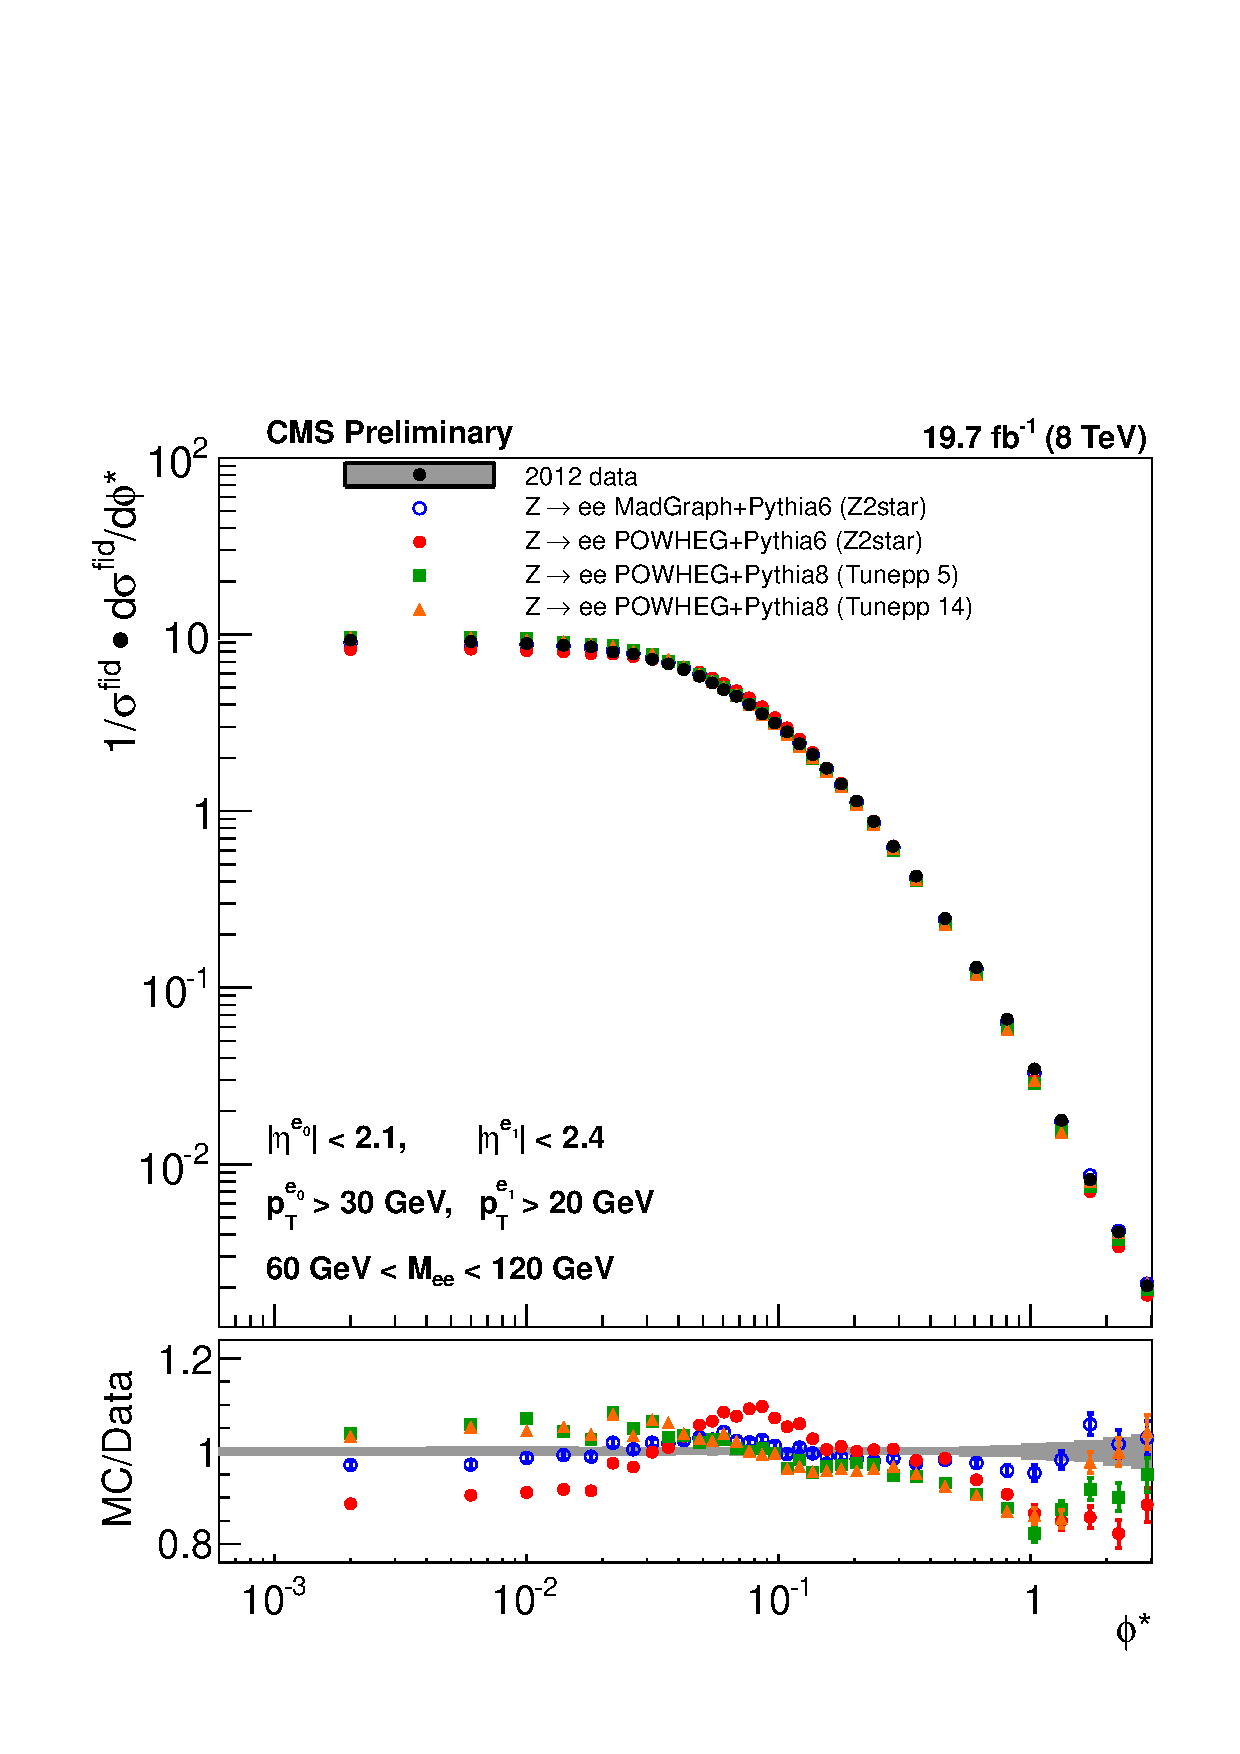
\includegraphics[width=\textwidth]{figures/ZShape_elec_PH_Norm_Dressed.pdf}
    \caption[
        The normalized differential cross section with respects to \phistar for
        \Ztoee events in our fiducial region from data and \MADGRAPH and
        \POWHEG unfolded with \POWHEG.
    ]{
        The normalized differential cross section with respects to \phistar for
        \Ztoee events in our fiducial region from data and \MADGRAPH and
        \POWHEG unfolded with \POWHEG. A close up of the lower plot is shown in
        \FIG~\ref{fig:results_ratio_norm_powheg}.
    }
    \label{fig:results_norm_powheg}
\end{figure}

\begin{figure}[!htbp]
    \centering
    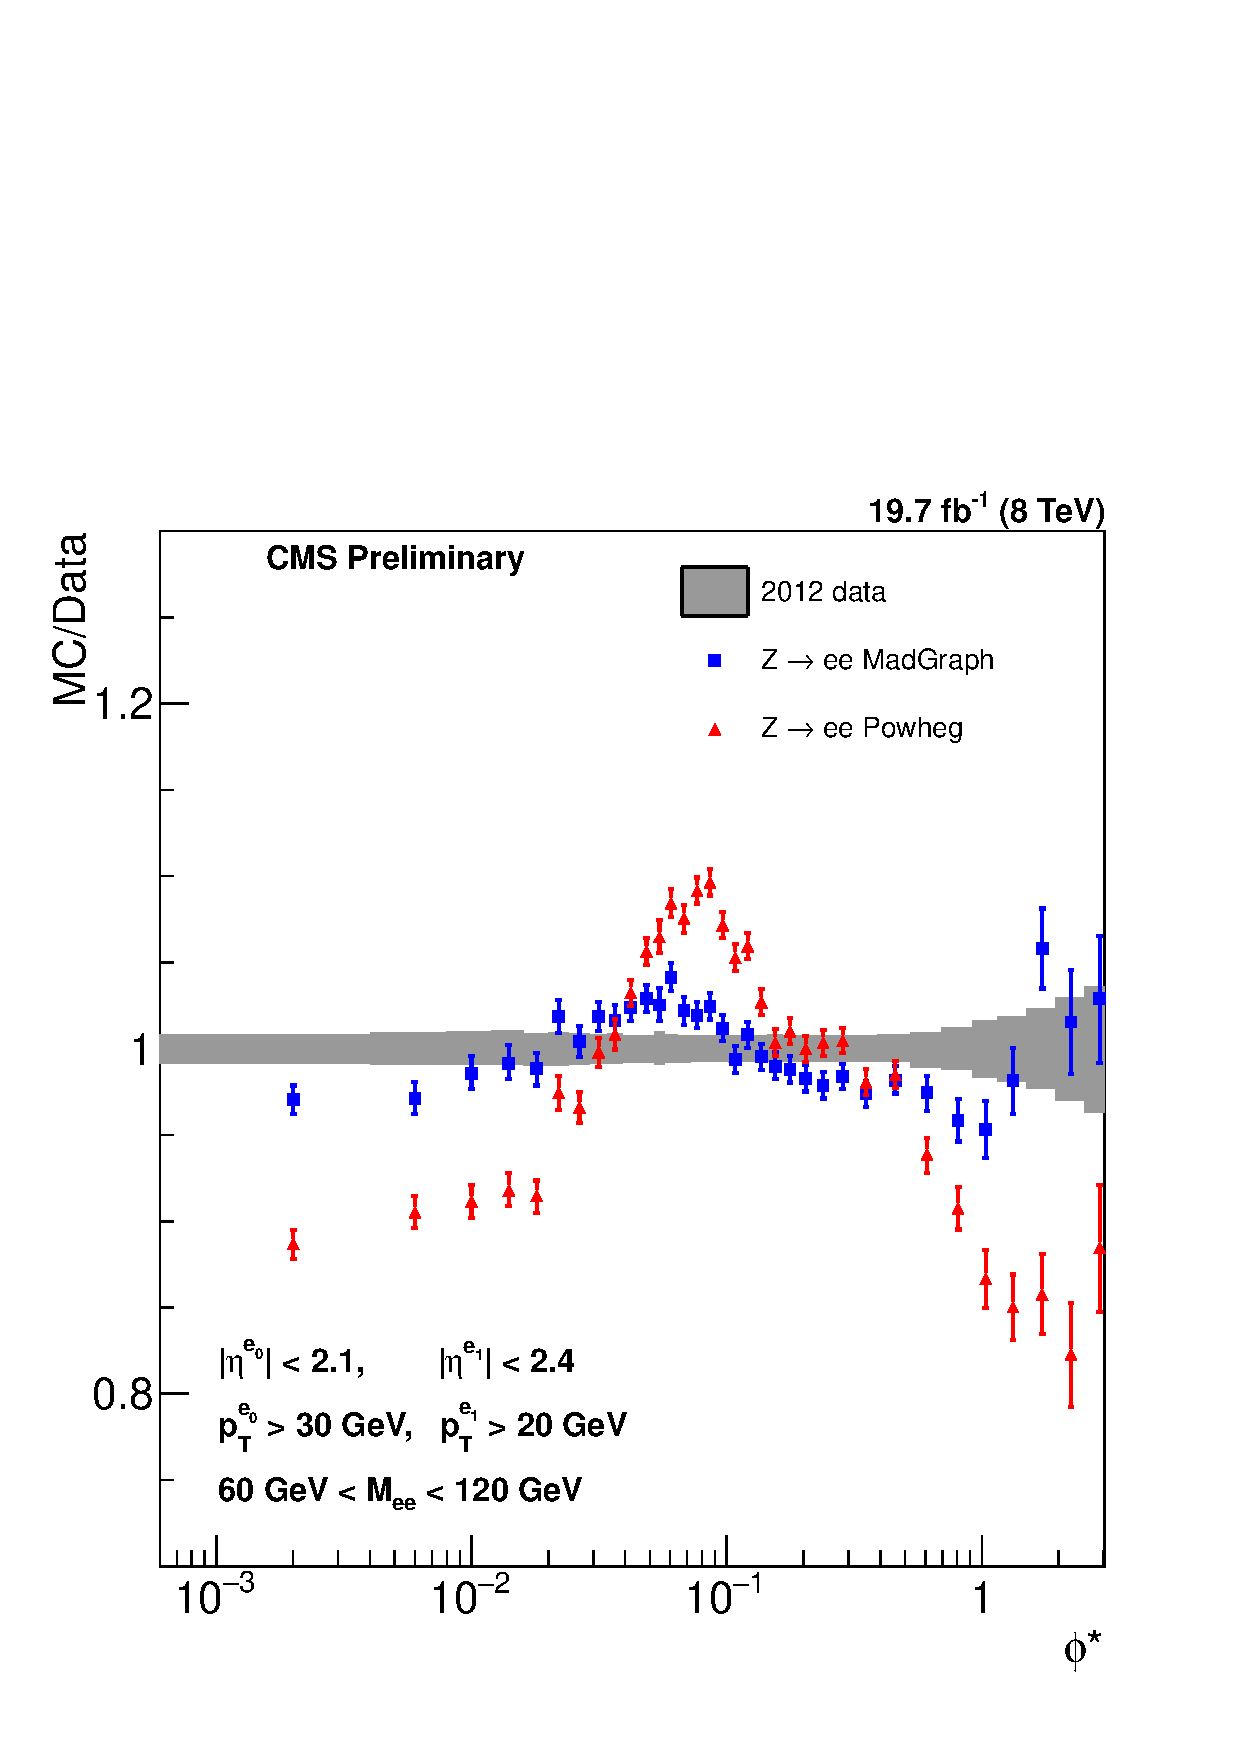
\includegraphics[width=\textwidth]{figures/ZShape_Ratioelec_PH_Norm_Dressed.pdf}
    \caption[
        Close up of the ratio plot from \FIG~\ref{fig:results_norm} for the
        normalized cross section measurement.
    ]{
        Close up of the ratio plot from \FIG~\ref{fig:results_norm} for the
        normalized cross section measurement unfolded with \POWHEG. The error
        band indicates the uncertainty in the data, while the square points
        show the ratio of \MADGRAPH over data, and the triangle points show the
        ratio of \POWHEG over data.
    }
    \label{fig:results_ratio_norm_powheg}
\end{figure}

% tab:results_norm_powheg
\begin{table}
    \spacerows{1.05}
    \begin{center}
        \begin{tabular}{@{}l r r r@{}}
            \toprule
            \phistar range & Data & \MADGRAPH & \POWHEG \\
            \midrule
            0.000--0.004  &  $9.29     \pm  0.08$     &  $9.01     \pm  0.02$     &  $8.24     \pm  0.05$     \\
            0.004--0.008  &  $9.12     \pm  0.08$     &  $8.86     \pm  0.02$     &  $8.26     \pm  0.05$     \\
            0.008--0.012  &  $8.89     \pm  0.09$     &  $8.76     \pm  0.02$     &  $8.10     \pm  0.05$     \\
            0.012--0.016  &  $8.68     \pm  0.09$     &  $8.61     \pm  0.02$     &  $7.97     \pm  0.05$     \\
            0.016--0.020  &  $8.51     \pm  0.08$     &  $8.42     \pm  0.02$     &  $7.79     \pm  0.05$     \\
            0.020--0.024  &  $7.95     \pm  0.08$     &  $8.10     \pm  0.02$     &  $7.75     \pm  0.05$     \\
            0.024--0.029  &  $7.75     \pm  0.07$     &  $7.78     \pm  0.02$     &  $7.48     \pm  0.04$     \\
            0.029--0.034  &  $7.23     \pm  0.06$     &  $7.37     \pm  0.02$     &  $7.22     \pm  0.04$     \\
            0.034--0.039  &  $6.81     \pm  0.06$     &  $6.93     \pm  0.02$     &  $6.87     \pm  0.04$     \\
            0.039--0.045  &  $6.33     \pm  0.05$     &  $6.48     \pm  0.02$     &  $6.53     \pm  0.04$     \\
            0.045--0.052  &  $5.80     \pm  0.04$     &  $5.97     \pm  0.01$     &  $6.12     \pm  0.03$     \\
            0.052--0.057  &  $5.32     \pm  0.05$     &  $5.45     \pm  0.02$     &  $5.66     \pm  0.04$     \\
            0.057--0.064  &  $4.87     \pm  0.04$     &  $5.07     \pm  0.01$     &  $5.28     \pm  0.03$     \\
            0.064--0.072  &  $4.47     \pm  0.04$     &  $4.57     \pm  0.01$     &  $4.80     \pm  0.03$     \\
            0.072--0.081  &  $4.01     \pm  0.03$     &  $4.09     \pm  0.01$     &  $4.38     \pm  0.02$     \\
            0.081--0.091  &  $3.55     \pm  0.03$     &  $3.640    \pm  0.010$    &  $3.90     \pm  0.02$     \\
            0.091--0.102  &  $3.15     \pm  0.02$     &  $3.192    \pm  0.009$    &  $3.38     \pm  0.02$     \\
            0.102--0.114  &  $2.81     \pm  0.02$     &  $2.795    \pm  0.008$    &  $2.96     \pm  0.02$     \\
            0.114--0.128  &  $2.41     \pm  0.02$     &  $2.426    \pm  0.007$    &  $2.55     \pm  0.02$     \\
            0.128--0.145  &  $2.09     \pm  0.02$     &  $2.079    \pm  0.006$    &  $2.14     \pm  0.01$     \\
            0.145--0.165  &  $1.75     \pm  0.01$     &  $1.730    \pm  0.005$    &  $1.75     \pm  0.01$     \\
            0.165--0.189  &  $1.42     \pm  0.01$     &  $1.406    \pm  0.004$    &  $1.438    \pm  0.009$    \\
            0.189--0.219  &  $1.141    \pm  0.009$    &  $1.121    \pm  0.003$    &  $1.140    \pm  0.007$    \\
            0.219--0.258  &  $0.874    \pm  0.007$    &  $0.855    \pm  0.002$    &  $0.877    \pm  0.006$    \\
            0.258--0.312  &  $0.632    \pm  0.005$    &  $0.622    \pm  0.002$    &  $0.635    \pm  0.004$    \\
            0.312--0.391  &  $0.428    \pm  0.003$    &  $0.417    \pm  0.001$    &  $0.420    \pm  0.003$    \\
            0.391--0.524  &  $0.247    \pm  0.002$    &  $0.2421   \pm  0.0007$   &  $0.243    \pm  0.002$    \\
            0.524--0.695  &  $0.130    \pm  0.001$    &  $0.1271   \pm  0.0004$   &  $0.1224   \pm  0.0010$   \\
            0.695--0.918  &  $0.0663   \pm  0.0008$   &  $0.0635   \pm  0.0003$   &  $0.0602   \pm  0.0006$   \\
            0.918--1.153  &  $0.0347   \pm  0.0006$   &  $0.0330   \pm  0.0002$   &  $0.0300   \pm  0.0004$   \\
            1.153--1.496  &  $0.0177   \pm  0.0003$   &  $0.0174   \pm  0.0001$   &  $0.0151   \pm  0.0003$   \\
            1.496--1.947  &  $0.0082   \pm  0.0002$   &  $0.00865  \pm  0.00007$  &  $0.0070   \pm  0.0002$   \\
            1.947--2.522  &  $0.0041   \pm  0.0001$   &  $0.00420  \pm  0.00004$  &  $0.00340  \pm  0.00009$  \\
            2.522--3.277  &  $0.00205  \pm  0.00007$  &  $0.00211  \pm  0.00003$  &  $0.00181  \pm  0.00006$  \\
            \bottomrule
        \end{tabular}
    \end{center}
    \caption[
        The normalized differential cross section in \pb with respects to
        \phistar for \Ztoee events in our fiducial region from data unfolded
        with \POWHEG.
    ]{
        The normalized differential cross section in \pb with respects to
        \phistar for \Ztoee events in our fiducial region from data unfolded
        with \POWHEG, and the same distributions in \MADGRAPH and \POWHEG.
        These results are shown graphically in \cref{fig:results_norm_powheg}.
    }
    \label{tab:results_norm_powheg}
\end{table}



% Bibliography
\bibliography{thesis}

% Appendices
\appendix
\chapter{Other Measurements Using \Dressed Electrons}
\label{app:dressed_measurements}

\section{Uncertainty Figures}

The values of the various uncertainties in each \phistar bin are presented in the
figures that follow. \Cref{fig:sys_uncert_norm} shows the uncertainties in the
normalized \phistar cross section in data unfolded with \MADGRAPH while
\cref{fig:sys_uncert_norm_powheg} shows the uncertainties in the data unfolded
with \PPsixZtwo. The uncertainties on the normalized \phistar cross section in
\MADGRAPH and \POWHEG are shown in
\cref{fig:madgraph_uncert_norm,fig:powheg_uncert_norm}, respectively. All of
these values are presented in tables in \cref{app:uncertainty_tables}.

% Absolute

% fig:sys_uncert_abs
\begin{figure}[!p]
    \centering
    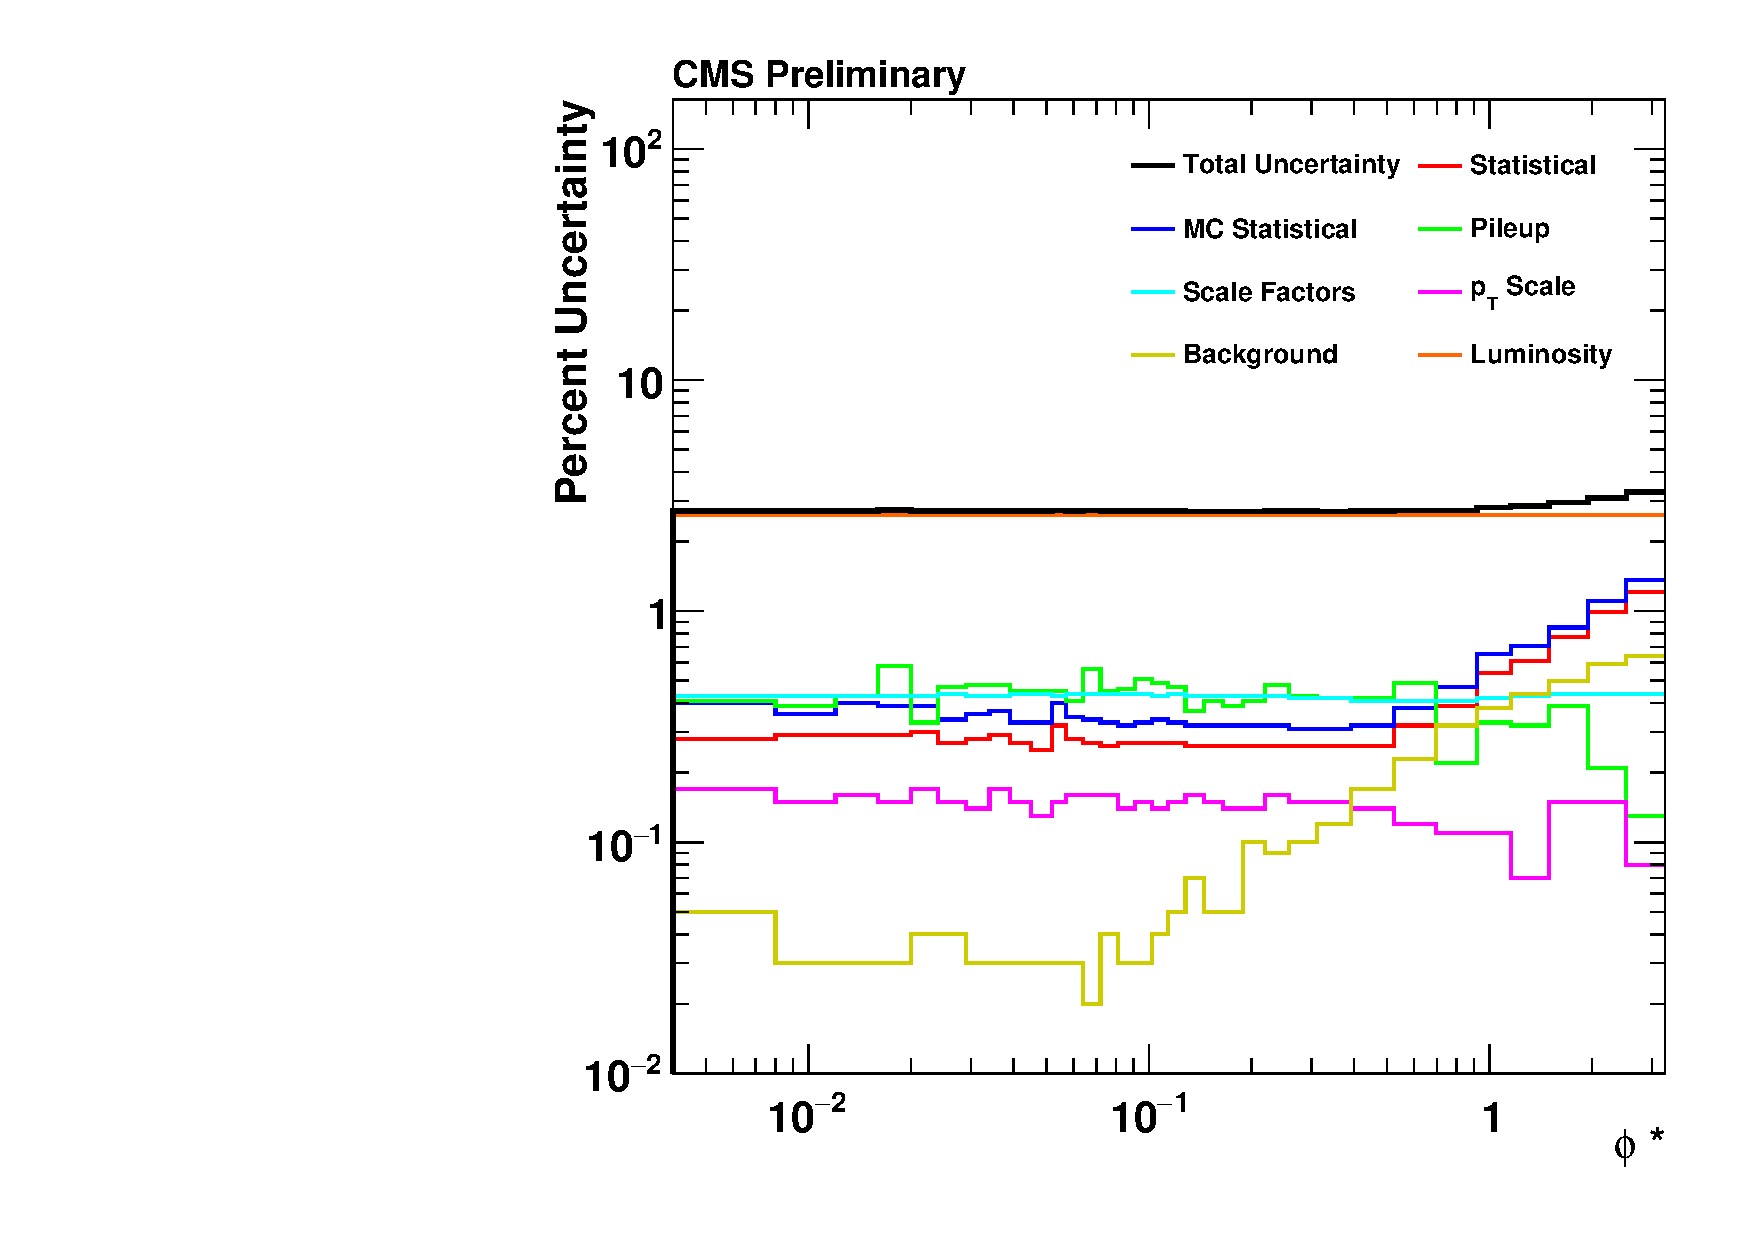
\includegraphics[width=\textwidth]{figures/data_uncertainty_absolute.pdf}
    \caption[
        Fractional errors (in \%) for the absolute cross section measurement
        made with data unfolded with \MADGRAPH.
    ]{
        Fractional errors (in \%) for the absolute cross section measurement
        made with data unfolded with \MADGRAPH. The total value is the sum in
        quadrature of all the other values. These uncertainties are also
        presented in tabular form in \cref{tab:sys_uncert_abs}.
    }
    \label{fig:sys_uncert_abs}
\end{figure}


% fig:sys_uncert_abs_powheg
\begin{figure}[!p]
    \centering
    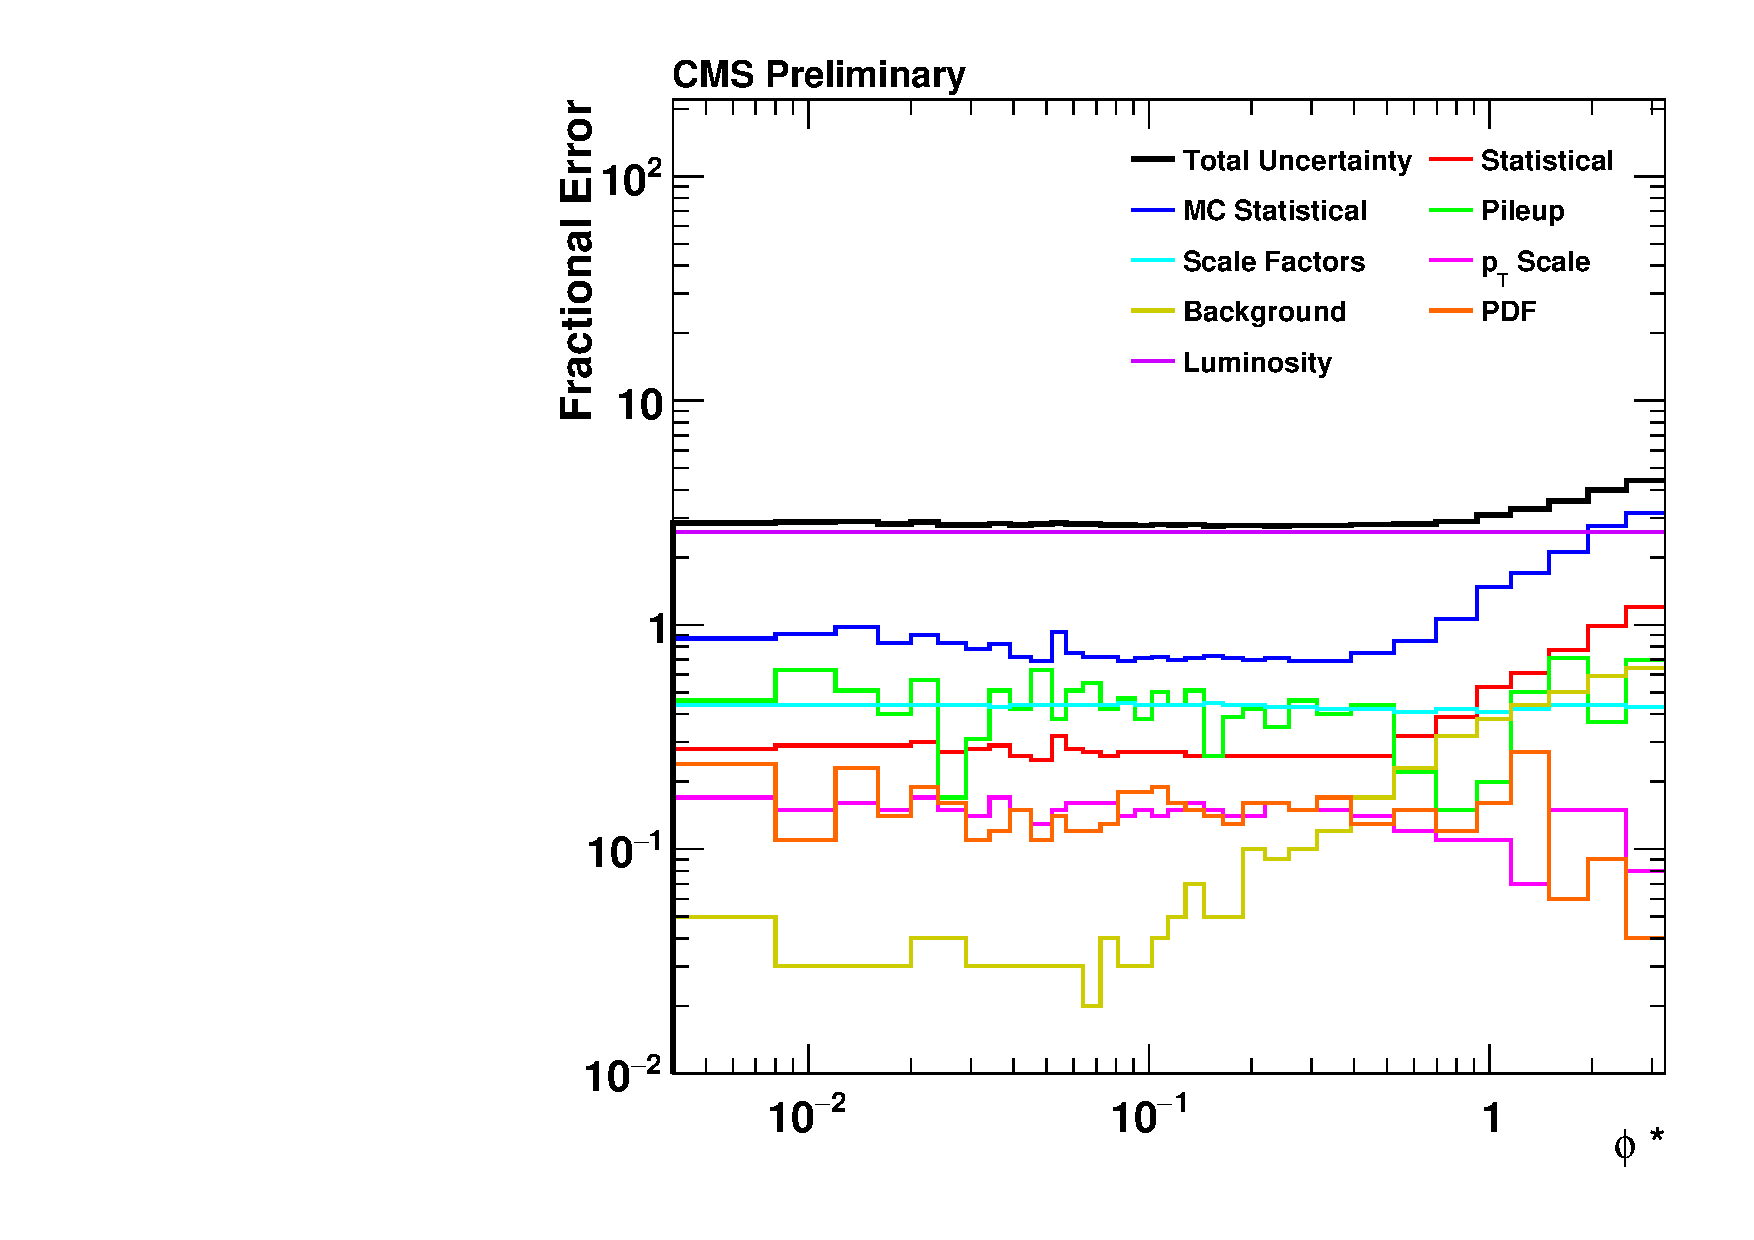
\includegraphics[width=\textwidth]{figures/data_uncertainty_absolute_powheg_unfolded.pdf}
    \caption[
        Fractional errors (in \%) for the absolute cross section measurement
        made with data unfolded with \POWHEG.
    ]{
        Fractional errors (in \%) for the absolute cross section measurement
        made with data unfolded with \POWHEG. The total value is the sum in
        quadrature of all the other values. These uncertainties are also
        presented in tabular form in \cref{tab:sys_uncert_abs_powheg}.
    }
    \label{fig:sys_uncert_abs_powheg}
\end{figure}


% fig:madgraph_uncert_abs
\begin{figure}[!htbp]
    \centering
    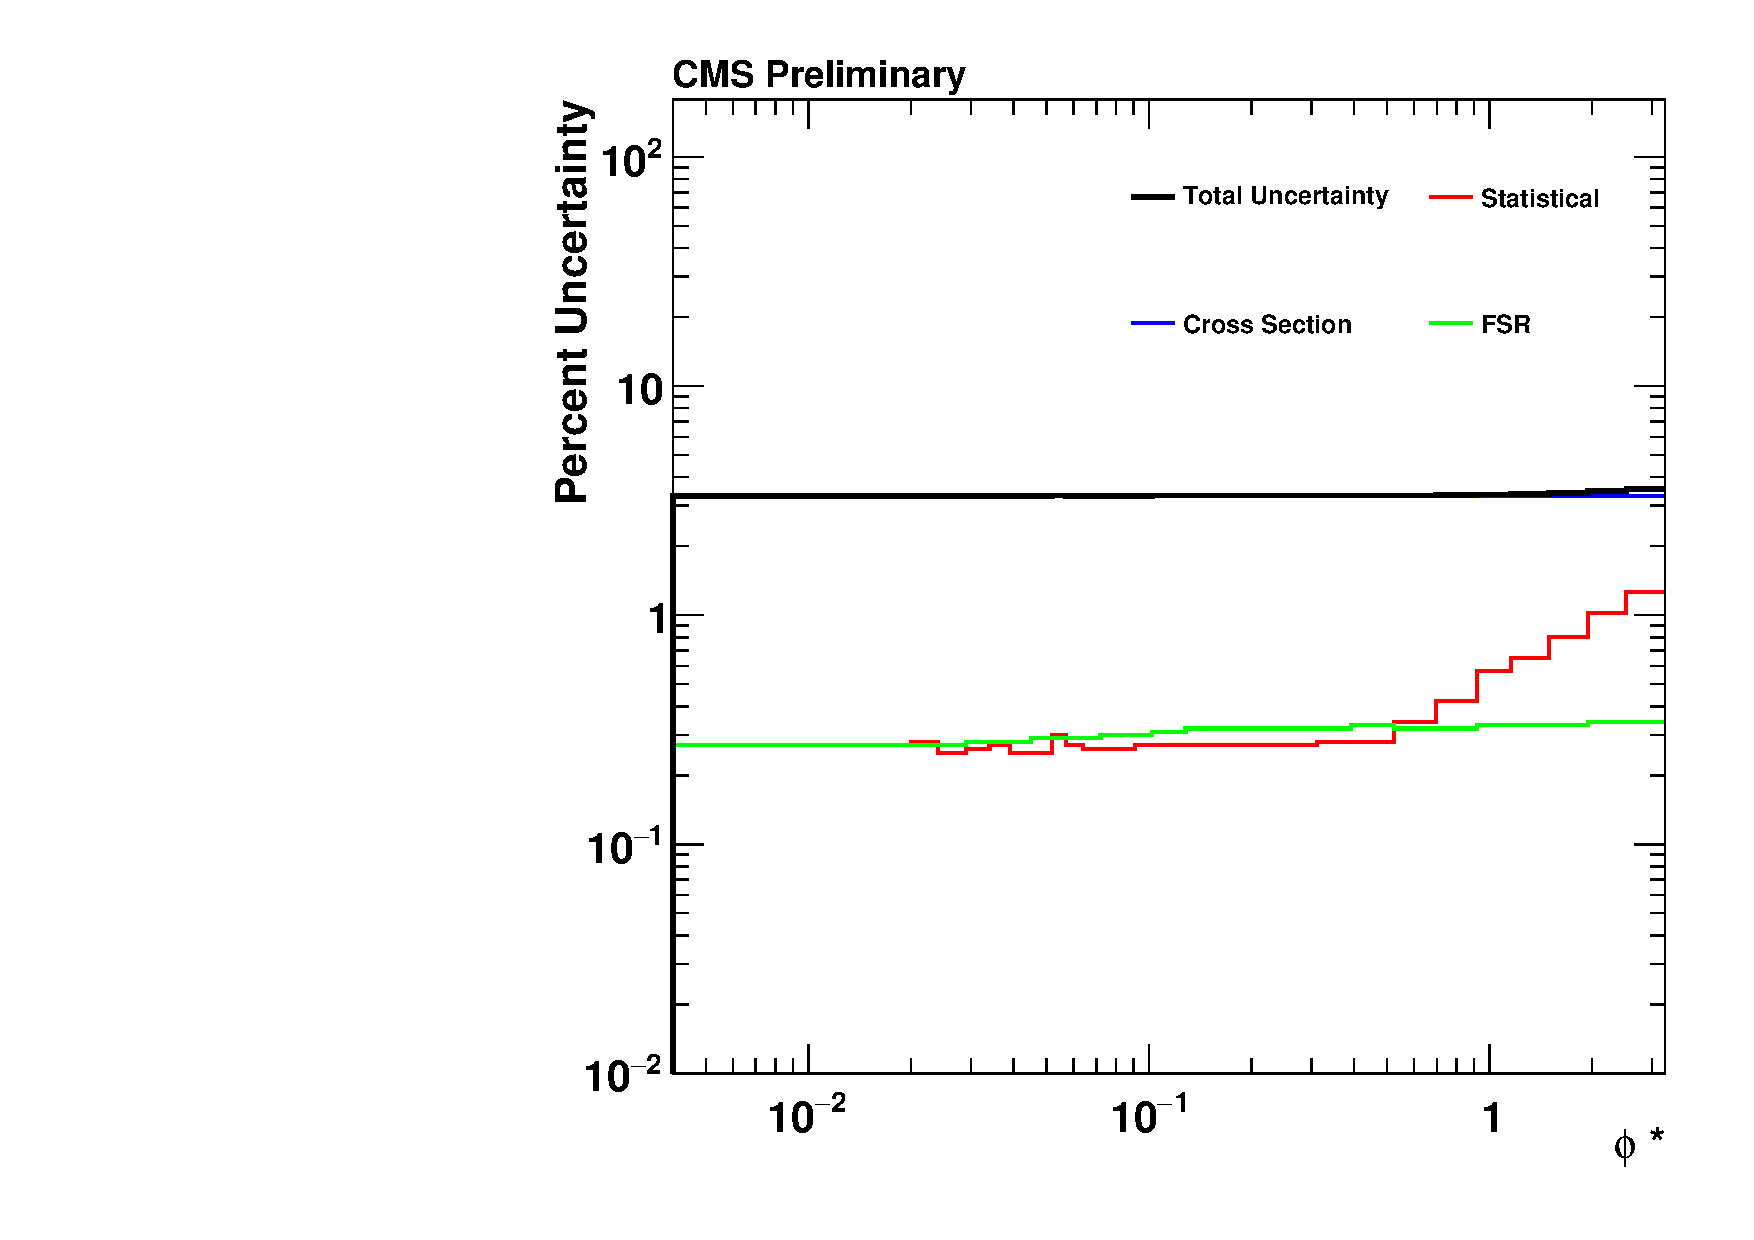
\includegraphics[width=\textwidth]{figures/madgraph_uncertainty_absolute.pdf}
    \caption[
        Fractional errors (in \%) for the absolute cross section from the
        \MADGRAPH MC sample.
    ]{
        Fractional errors (in \%) for the absolute cross section from the
        \MADGRAPH MC sample. These uncertainties are also presented in tabular
        form in \TAB~\ref{tab:madgraph_uncert_abs}.
    }
    \label{fig:madgraph_uncert_abs}
\end{figure}


% fig:powheg_uncert_abs
\begin{figure}[!p]
    \centering
    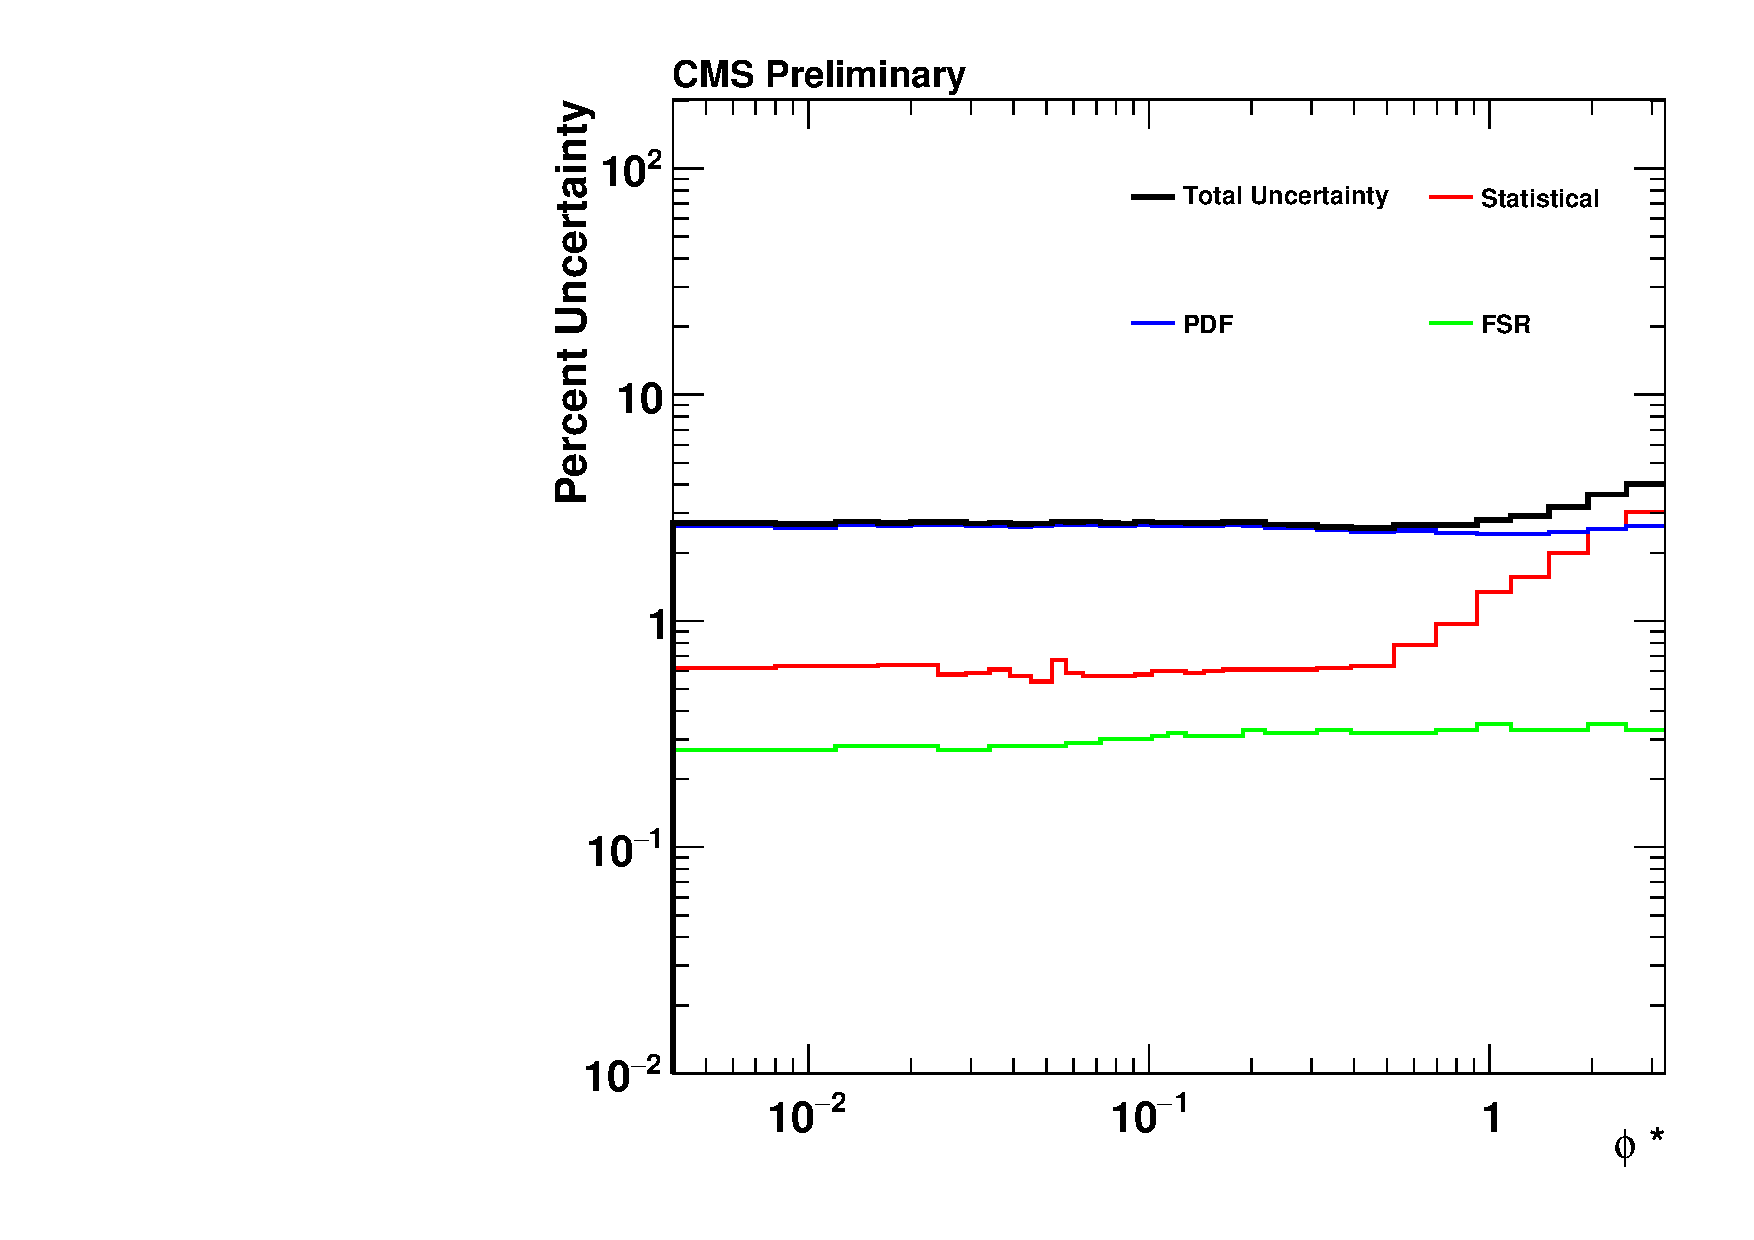
\includegraphics[width=\textwidth]{figures/powheg_uncertainty_absolute.pdf}
    \caption[
        The uncertainties for the absolute cross section from the \POWHEG MC
        sample.
    ]{
        The uncertainties (in \%) for the absolute cross section from the
        \POWHEG MC sample. These uncertainties are also presented in tabular
        form in \cref{tab:powheg_uncert_abs}.
    }
    \label{fig:powheg_uncert_abs}
\end{figure}



\section{Absolute Differential Cross Section}
\label{sec:results_abs}

The absolute differential cross section measurement using data unfolded with
\MADGRAPH is shown in \cref{fig:results_abs} and given in tabular form in
\cref{tab:results_abs}. The lower plot in \cref{fig:results_abs} is
shown in more detail in \cref{fig:results_ratio_abs}. As previously
discussed in this chapter, the primary uncertainty on the data distribution is
from the integrated luminosity. The primary uncertainty for the
\MADGRAPH sample is the \FEWZ calculated overall cross section used to scale
the distribution, while the primary uncertainty for the \POWHEG samples is the
uncertainty calculated by varying the \CTten PDF weights.

% fig:results_abs and fig:results_ratio_abs
\begin{figure}[!p]
    \centering
    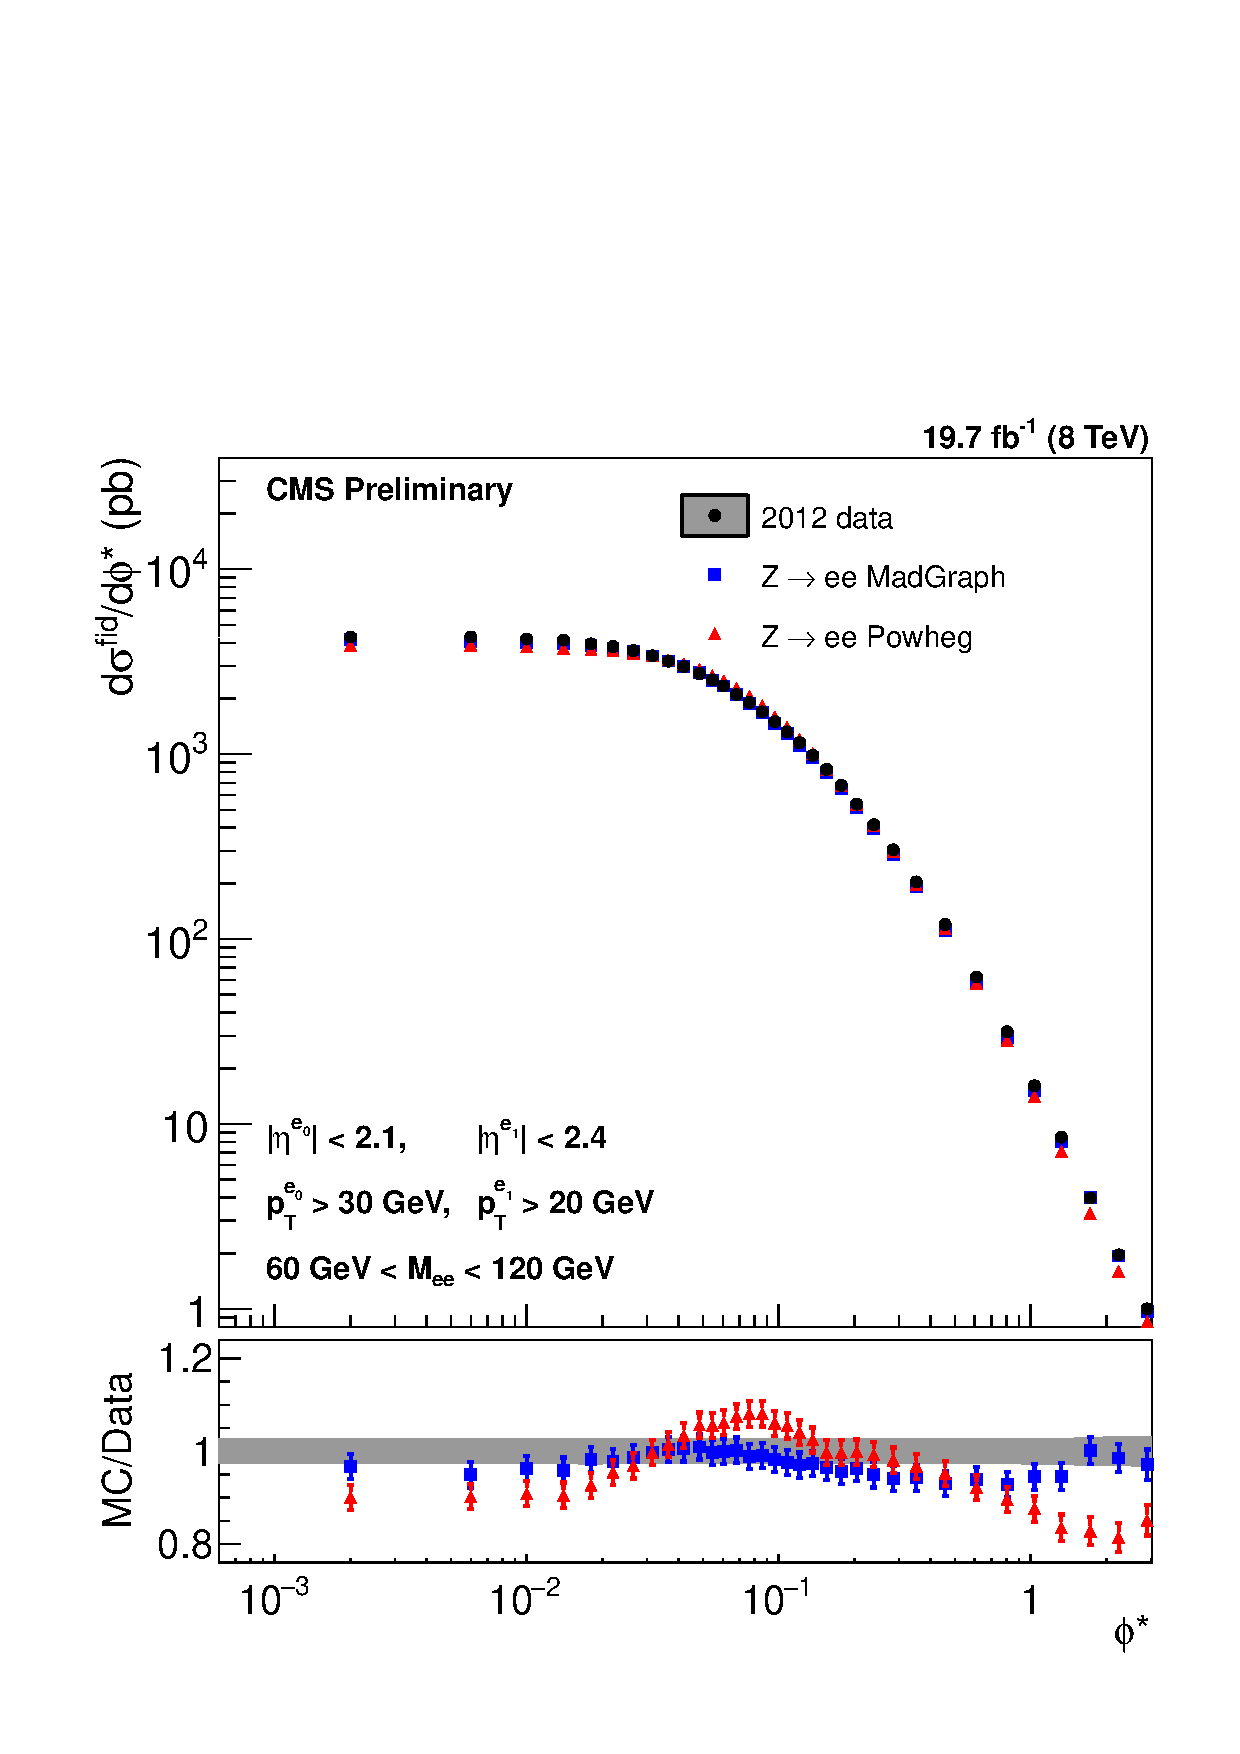
\includegraphics[width=\textwidth]{figures/ZShape_elec_Abs_Dressed.pdf}
    \caption[
        The absolute differential cross section with respects to \phistar for
        \Ztoee events in our fiducial region from data unfolded with \MADGRAPH,
        and the same distributions in \MADGRAPH and \POWHEG.
    ]{
        The absolute differential cross section with respects to \phistar for
        \Ztoee events in our fiducial region from data unfolded with \MADGRAPH,
        and the same distributions in \MADGRAPH and \POWHEG. A close up of the
        lower plot is shown in \cref{fig:results_ratio_abs}.
    }
    \label{fig:results_abs}
\end{figure}

\begin{figure}[!p]
    \centering
    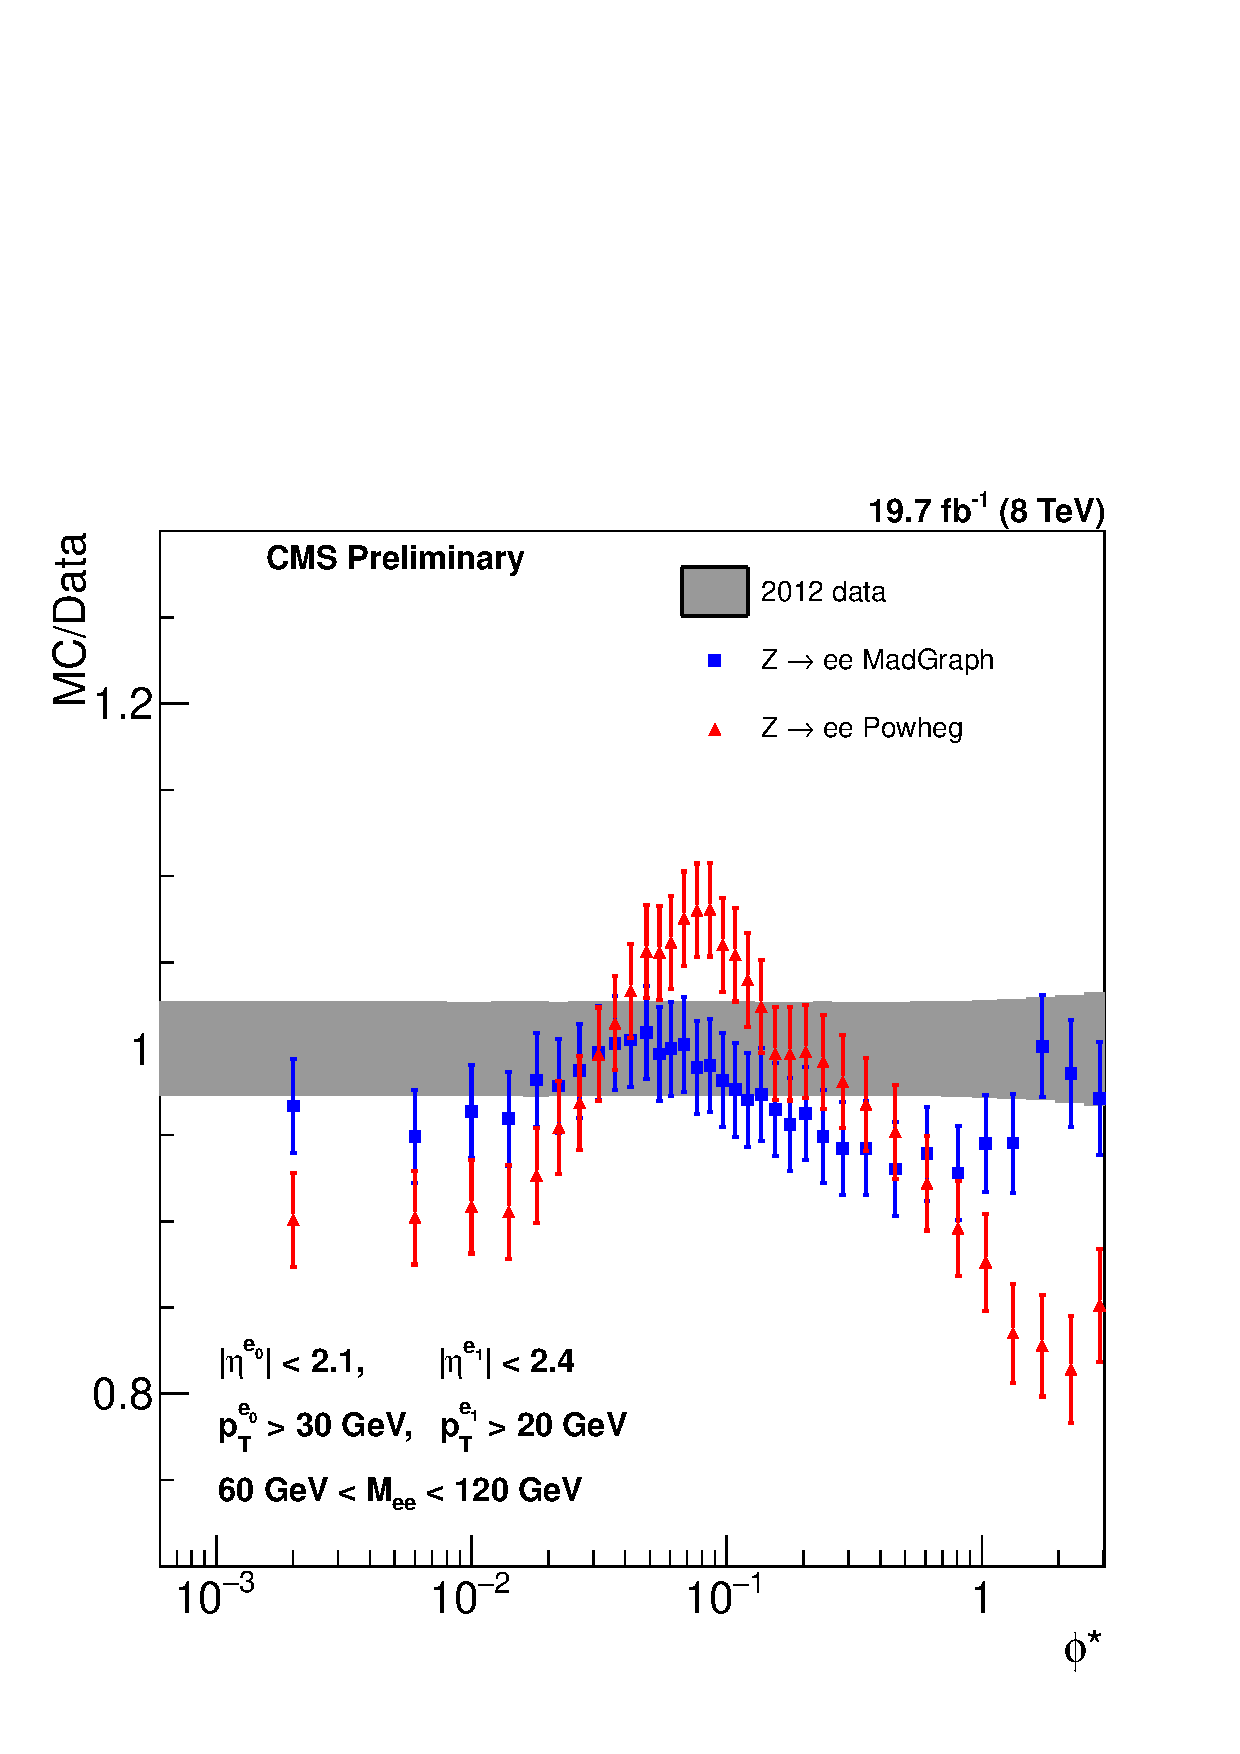
\includegraphics[width=\textwidth]{figures/ZShape_Ratioelec_Abs_Dressed.pdf}
    \caption[
        Close up of the ratio plot from \cref{fig:results_abs} for the
        absolute cross section measurement unfolded with \MADGRAPH.
    ]{
        Close up of the ratio plot from \cref{fig:results_abs} for the
        absolute cross section measurement unfolded with \MADGRAPH. The error
        band indicates the uncertainty in the data, while the square points
        show the ratio of \MADGRAPH over data, and the triangle points show the
        ratio of \POWHEG over data.
    }
    \label{fig:results_ratio_abs}
\end{figure}

% tab:results_abs
\begin{table}
    \spacerows{1.05}
    \begin{center}
        \begin{tabular}{@{}l r r r@{}}
            \toprule
            \phistar range & Data $(\pb)$ & \MADGRAPH $(\pb)$ & \POWHEG $(\pm)$ \\
            \midrule
            0.000--0.004  &  $4297  \pm  117$   &  $4155  \pm  138$   &  $3871  \pm  105$   \\
            0.004--0.008  &  $4302  \pm  117$   &  $4083  \pm  136$   &  $3881  \pm  105$   \\
            0.008--0.012  &  $4190  \pm  113$   &  $4037  \pm  134$   &  $3806  \pm  102$   \\
            0.012--0.016  &  $4137  \pm  113$   &  $3969  \pm  132$   &  $3746  \pm  103$   \\
            0.016--0.020  &  $3951  \pm  109$   &  $3879  \pm  129$   &  $3660  \pm  99$    \\
            0.020--0.024  &  $3816  \pm  103$   &  $3734  \pm  124$   &  $3642  \pm  100$   \\
            0.024--0.029  &  $3632  \pm  99$    &  $3586  \pm  119$   &  $3518  \pm  96$    \\
            0.029--0.034  &  $3404  \pm  93$    &  $3396  \pm  113$   &  $3393  \pm  92$    \\
            0.034--0.039  &  $3182  \pm  87$    &  $3192  \pm  106$   &  $3229  \pm  88$    \\
            0.039--0.045  &  $2971  \pm  81$    &  $2987  \pm  99$    &  $3071  \pm  83$    \\
            0.045--0.052  &  $2724  \pm  74$    &  $2750  \pm  91$    &  $2878  \pm  78$    \\
            0.052--0.057  &  $2521  \pm  69$    &  $2514  \pm  84$    &  $2662  \pm  73$    \\
            0.057--0.064  &  $2335  \pm  63$    &  $2335  \pm  78$    &  $2479  \pm  68$    \\
            0.064--0.072  &  $2099  \pm  57$    &  $2104  \pm  70$    &  $2257  \pm  62$    \\
            0.072--0.081  &  $1904  \pm  52$    &  $1883  \pm  63$    &  $2057  \pm  56$    \\
            0.081--0.091  &  $1694  \pm  46$    &  $1678  \pm  56$    &  $1831  \pm  49$    \\
            0.091--0.102  &  $1498  \pm  41$    &  $1471  \pm  49$    &  $1589  \pm  44$    \\
            0.102--0.114  &  $1320  \pm  36$    &  $1288  \pm  43$    &  $1392  \pm  38$    \\
            0.114--0.128  &  $1152  \pm  31$    &  $1118  \pm  37$    &  $1198  \pm  33$    \\
            0.128--0.145  &  $984   \pm  27$    &  $958   \pm  32$    &  $1008  \pm  27$    \\
            0.145--0.165  &  $827   \pm  22$    &  $797   \pm  27$    &  $824   \pm  22$    \\
            0.165--0.189  &  $678   \pm  18$    &  $648   \pm  22$    &  $676   \pm  18$    \\
            0.189--0.219  &  $537   \pm  15$    &  $517   \pm  17$    &  $536   \pm  15$    \\
            0.219--0.258  &  $415   \pm  11$    &  $394   \pm  13$    &  $412   \pm  11$    \\
            0.258--0.312  &  $304   \pm  8$     &  $287   \pm  10$    &  $298   \pm  8$     \\
            0.312--0.391  &  $204   \pm  6$     &  $192   \pm  6$     &  $197   \pm  5$     \\
            0.391--0.524  &  $120   \pm  3$     &  $112   \pm  4$     &  $114   \pm  3$     \\
            0.524--0.695  &  $62    \pm  2$     &  $59    \pm  2$     &  $58    \pm  2$     \\
            0.695--0.918  &  $31.6  \pm  0.9$   &  $29.3  \pm  1.0$   &  $28.3  \pm  0.7$   \\
            0.918--1.153  &  $16.1  \pm  0.5$   &  $15.2  \pm  0.5$   &  $14.1  \pm  0.4$   \\
            1.153--1.496  &  $8.5   \pm  0.2$   &  $8.0   \pm  0.3$   &  $7.1   \pm  0.2$   \\
            1.496--1.947  &  $4.0   \pm  0.1$   &  $4.0   \pm  0.1$   &  $3.3   \pm  0.1$   \\
            1.947--2.522  &  $1.96  \pm  0.06$  &  $1.93  \pm  0.07$  &  $1.60  \pm  0.06$  \\
            2.522--3.277  &  $1.00  \pm  0.03$  &  $0.97  \pm  0.03$  &  $0.85  \pm  0.03$  \\
            \bottomrule
        \end{tabular}
    \end{center}
    \caption[
        Differential cross-section in \pb with respect to \phistar of \Ztoee.
    ]{
        Differential cross-section in \pb with respect to \phistar of \Ztoee in
        our fiducial region in data and as generated by \MADGRAPH and \POWHEG.
        These results are shown graphically in figure~\ref{fig:result_abs}.
    }
    \label{tab:results_abs}
\end{table}


The absolute differential cross section measurement using data unfolded with
\PPsixZtwo is shown in \cref{fig:results_abs_powheg} and given in tabular form
in \cref{tab:results_abs_powheg}. The lower plot in
\cref{fig:results_abs_powheg} is shown in more detail in
\cref{fig:results_ratio_abs_powheg}. The primary uncertainty on the data
distribution is still from the integrated luminosity, although the MC
statistical uncertainty is larger in the highest \phistar bins.

% fig:results_abs_powheg and fig:results_ratio_abs_powheg
\begin{figure}[!p]
    \centering
    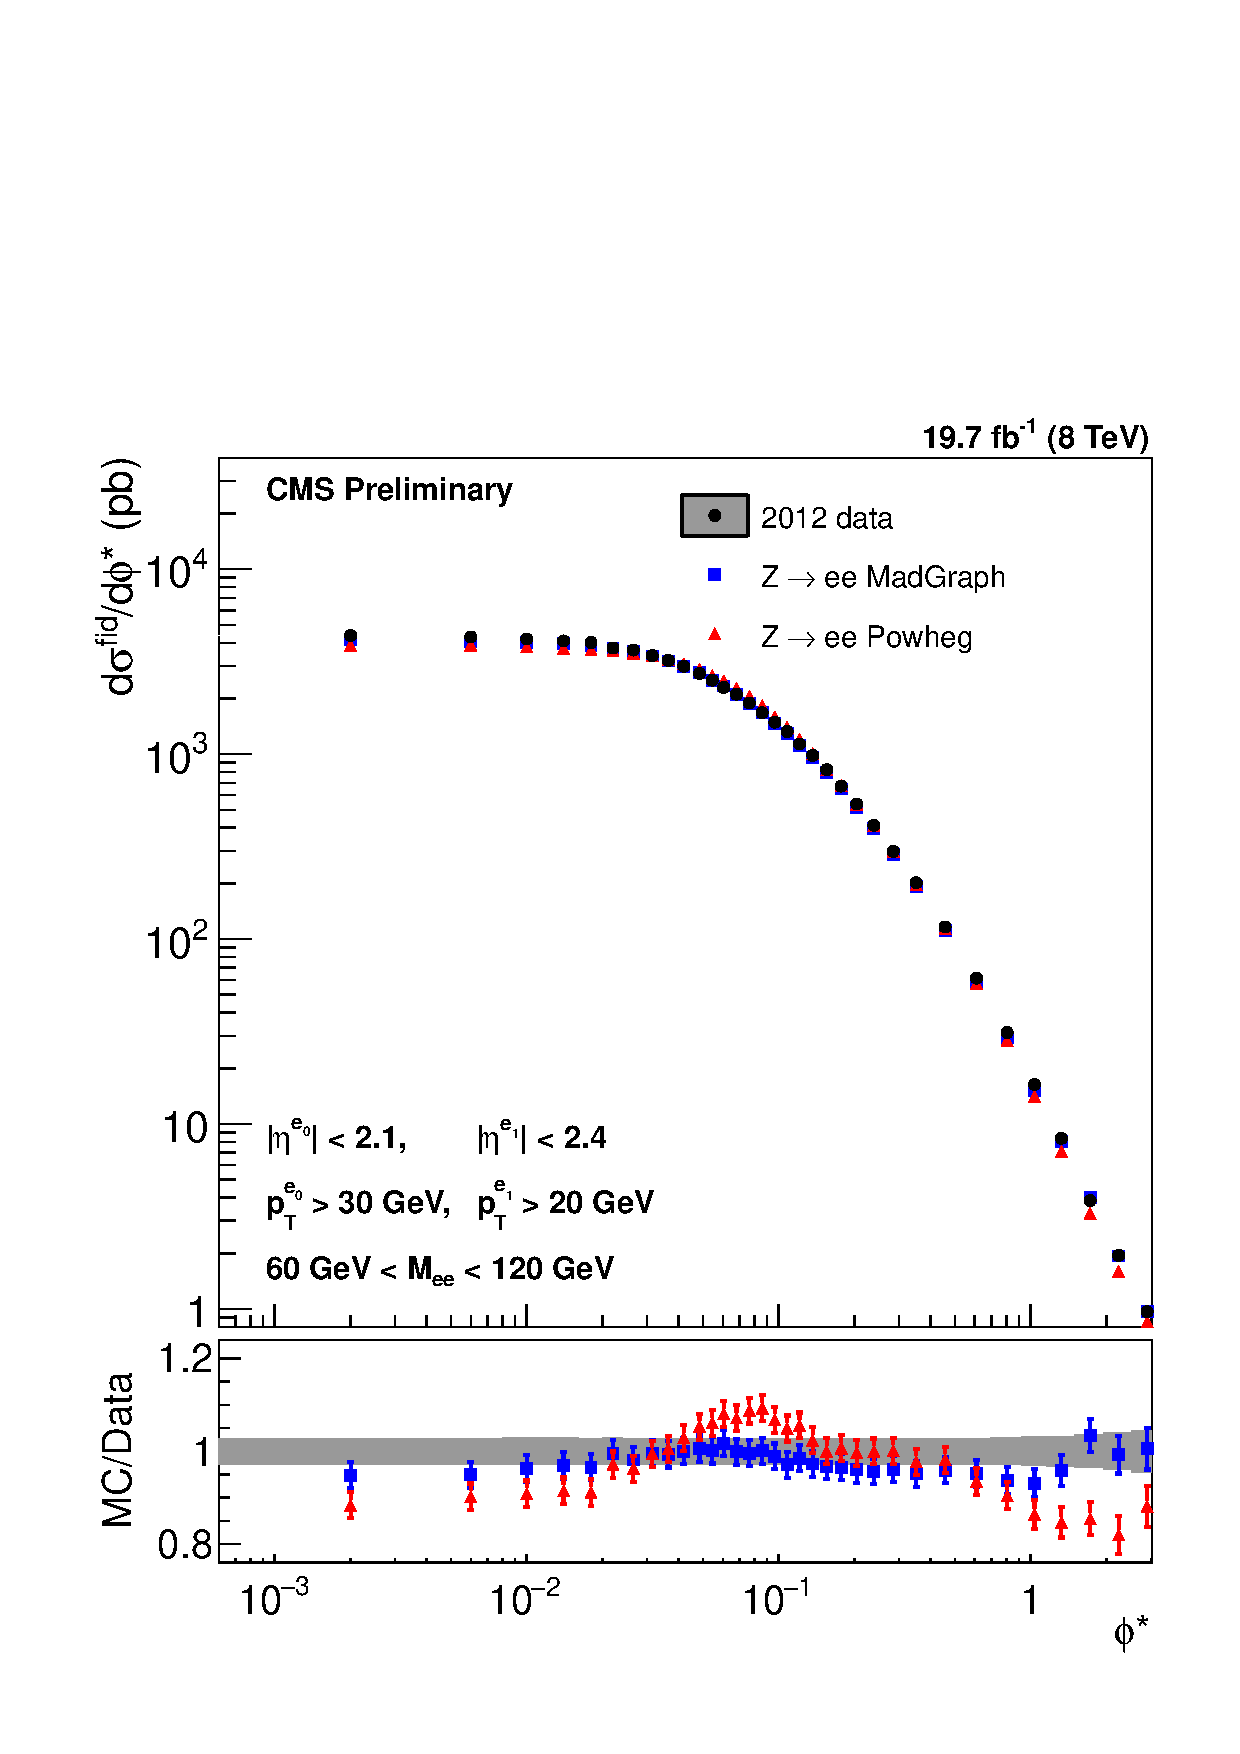
\includegraphics[width=\textwidth]{figures/ZShape_elec_PH_Abs_Dressed.pdf}
    \caption[
        The absolute differential cross section with respects to \phistar for
        \Ztoee events in our fiducial region from data unfolded with
        \PPsixZtwo.
    ]{
        The absolute differential cross section with respects to \phistar for
        \Ztoee events in our fiducial region from data unfolded with
        \PPsixZtwo, and the same distributions in \MADGRAPH and \PPsixZtwo. A
        close up of the lower plot is shown in
        \cref{fig:results_ratio_abs_powheg}.
    }
    \label{fig:results_abs_powheg}
\end{figure}

\begin{figure}[!p]
    \centering
    \includegraphics[width=\textwidth]{figures/ZShape_Ratioelec_PH_Abs_Dressed.pdf}
    \caption[
        Close up of the ratio plot from \cref{fig:results_abs_powheg} for the
        absolute cross section measurement unfolded with \PPsixZtwo.
    ]{
        Close up of the ratio plot from \cref{fig:results_abs_powheg} for the
        absolute cross section measurement unfolded with \PPsixZtwo. The error
        band indicates the uncertainty in the data, while the square points
        show the ratio of \MADGRAPH over data, and the triangle points show the
        ratio of \PPsixZtwo over data.
    }
    \label{fig:results_ratio_abs_powheg}
\end{figure}

% tab:results_abs_powheg
\begin{table}
    \spacerows{1.05}
    \begin{center}
        \begin{tabular}{@{}l r r r@{}}
            \toprule
            \phistar range & Data $(\pb)$ & \MADGRAPH $(\pb)$ & \POWHEG $(\pm)$ \\
            \midrule
            0.000--0.004  &  $4381  \pm  122$   &  $4155  \pm  138$   &  $3871  \pm  105$   \\
            0.004--0.008  &  $4302  \pm  122$   &  $4083  \pm  136$   &  $3881  \pm  105$   \\
            0.008--0.012  &  $4191  \pm  121$   &  $4037  \pm  134$   &  $3806  \pm  102$   \\
            0.012--0.016  &  $4096  \pm  118$   &  $3969  \pm  132$   &  $3746  \pm  103$   \\
            0.016--0.020  &  $4016  \pm  113$   &  $3879  \pm  129$   &  $3660  \pm  99$    \\
            0.020--0.024  &  $3751  \pm  108$   &  $3734  \pm  124$   &  $3642  \pm  100$   \\
            0.024--0.029  &  $3654  \pm  102$   &  $3586  \pm  119$   &  $3518  \pm  96$    \\
            0.029--0.034  &  $3412  \pm  95$    &  $3396  \pm  113$   &  $3393  \pm  92$    \\
            0.034--0.039  &  $3213  \pm  91$    &  $3192  \pm  106$   &  $3229  \pm  88$    \\
            0.039--0.045  &  $2985  \pm  83$    &  $2987  \pm  99$    &  $3071  \pm  83$    \\
            0.045--0.052  &  $2734  \pm  77$    &  $2750  \pm  91$    &  $2878  \pm  78$    \\
            0.052--0.057  &  $2509  \pm  71$    &  $2514  \pm  84$    &  $2662  \pm  73$    \\
            0.057--0.064  &  $2295  \pm  65$    &  $2335  \pm  78$    &  $2479  \pm  68$    \\
            0.064--0.072  &  $2107  \pm  59$    &  $2104  \pm  70$    &  $2257  \pm  62$    \\
            0.072--0.081  &  $1891  \pm  53$    &  $1883  \pm  63$    &  $2057  \pm  56$    \\
            0.081--0.091  &  $1676  \pm  47$    &  $1678  \pm  56$    &  $1831  \pm  49$    \\
            0.091--0.102  &  $1488  \pm  41$    &  $1471  \pm  49$    &  $1589  \pm  44$    \\
            0.102--0.114  &  $1327  \pm  37$    &  $1288  \pm  43$    &  $1392  \pm  38$    \\
            0.114--0.128  &  $1135  \pm  32$    &  $1118  \pm  37$    &  $1198  \pm  33$    \\
            0.128--0.145  &  $985   \pm  28$    &  $958   \pm  32$    &  $1008  \pm  27$    \\
            0.145--0.165  &  $824   \pm  23$    &  $797   \pm  27$    &  $824   \pm  22$    \\
            0.165--0.189  &  $671   \pm  19$    &  $648   \pm  22$    &  $676   \pm  18$    \\
            0.189--0.219  &  $538   \pm  15$    &  $517   \pm  17$    &  $536   \pm  15$    \\
            0.219--0.258  &  $412   \pm  11$    &  $394   \pm  13$    &  $412   \pm  11$    \\
            0.258--0.312  &  $298   \pm  8$     &  $287   \pm  10$    &  $298   \pm  8$     \\
            0.312--0.391  &  $202   \pm  6$     &  $192   \pm  6$     &  $197   \pm  5$     \\
            0.391--0.524  &  $116   \pm  3$     &  $112   \pm  4$     &  $114   \pm  3$     \\
            0.524--0.695  &  $61    \pm  2$     &  $59    \pm  2$     &  $58    \pm  2$     \\
            0.695--0.918  &  $31.3  \pm  0.9$   &  $29.3  \pm  1.0$   &  $28.3  \pm  0.7$   \\
            0.918--1.153  &  $16.4  \pm  0.5$   &  $15.2  \pm  0.5$   &  $14.1  \pm  0.4$   \\
            1.153--1.496  &  $8.4   \pm  0.3$   &  $8.0   \pm  0.3$   &  $7.1   \pm  0.2$   \\
            1.496--1.947  &  $3.9   \pm  0.1$   &  $4.0   \pm  0.1$   &  $3.3   \pm  0.1$   \\
            1.947--2.522  &  $1.95  \pm  0.08$  &  $1.93  \pm  0.07$  &  $1.60  \pm  0.06$  \\
            2.522--3.277  &  $0.97  \pm  0.04$  &  $0.97  \pm  0.03$  &  $0.85  \pm  0.03$  \\
            \bottomrule
        \end{tabular}
    \end{center}
    \caption[
        The absolute differential cross section in \pb with respects to
        \phistar for \Ztoee events in our fiducial region from data unfolded
        with \POWHEG.
    ]{
        The absolute differential cross section in \pb with respects to
        \phistar for \Ztoee events in our fiducial region from data unfolded
        with \POWHEG, and the same distributions in \MADGRAPH and \POWHEG.
        These results are shown graphically in
        figure~\ref{fig:results_abs_powheg}.
    }
    \label{tab:results_abs_powheg}
\end{table}


\chapter{Uncertainty Tables}
\label{app:uncertainty_tables}

The fractional uncertainty on the normalized cross section measurement in
\FIGS~\ref{fig:sys_uncert_norm}, \ref{fig:sys_uncert_norm_powheg},
\ref{fig:madgraph_uncert_norm}, and \ref{fig:powheg_uncert_norm}, and for the
absolute cross section measurement is shown in \FIGS~\ref{fig:sys_uncert_abs},
\ref{fig:sys_uncert_abs_powheg}, \ref{fig:madgraph_uncert_abs}, and
\ref{fig:powheg_uncert_abs}. In this appendix, the values of these
uncertainties are presented in tabular form.

\section{Explanation of the Columns}

The tables with information about the uncertainty on the data,
\TABS~\ref{tab:sys_uncert_norm}, \ref{tab:sys_uncert_norm_powheg},
\ref{tab:sys_uncert_abs}, and \ref{tab:sys_uncert_abs_powheg} contain the
following columns:

\begin{description}[noitemsep]

    \item[\phistar Range:] \hfill \\
        The range of \phistar values included in the bin.

    \item[Total Uncertainty (Total):] \hfill \\
        The sum in quadrature of the all of the uncertainties.

    \item[Statistical Uncertainty (Stat.):] \hfill \\
        The uncertainty due to the limited number of events in the data, as
        discussed in \SEC~\ref{ssec:stat_uncertainty}.

    \item[Total Systematic Uncertainty (Total Syst.):] \hfill \\
        The sum in quadrature of all of the systematic uncertainties including,
        for the absolute distribution, the luminosity uncertainty of
        \LumiUncertainty.

    \item[Monte Carlo Statistical Uncertainty (MC Stat.):] \hfill \\
        The uncertainty due to the limited number of events in the MC samples,
        as discussed in \SEC~\ref{ssec:mc_stat_uncertainty}.

    \item[Pileup Uncertainty (Pileup):] \hfill \\
        The uncertainty due to the pileup reweighting, as discussed in
        \SEC~\ref{ssec:pileup_uncertainty}.

    \item[Scale Factor Uncertainty (SF):] \hfill \\
        The uncertainty due to the scale factors, as discussed in
        \SEC~\ref{scale_factor_uncertainty}.

    \item[\pt Scale Uncertainty (\pt Scale):] \hfill \\
        The uncertainty due to \pt scale, as discussed in
        \SEC~\ref{ssec:pt_scale_uncertainty}.

    \item[Background Subtraction Uncertainty (Bkg.):] \hfill \\
        The uncertainty due to background subtraction, as discussed in
        \SEC~\ref{ssec:background_subtraction_uncertainty}.

\end{description}

The tables with information related to the uncertainty on the MC distributions,
\TABS~\ref{tab:madgraph_uncert_norm}, \ref{tab:powheg_uncert_norm},
\ref{tab:madgraph_uncert_abs}, and \ref{tab:powheg_uncert_abs}, have the
following columns:

\begin{description}[noitemsep]

    \item[\phistar Range:] \hfill \\
        The range of \phistar values included in the bin.

    \item[Total Uncertainty (Total):] \hfill \\
        The sum in quadrature of the all of the uncertainties.

    \item[Statistical Uncertainty (Stat.):] \hfill \\
        The uncertainty due to the limited number of events in the MC sample.

    \item[Parton Density Function (PDF):] \hfill \\
        The uncertainty due to choice of PDF used to generate the \POWHEG MC,
        as discussed in \SEC~\ref{ssec:pdf_uncertainties}.

    \item[Theoretical Cross Section Uncertainty (Cross Section):] \hfill \\
        The uncertainty in the theoretical cross section of the \MADGRAPH MC,
        as discussed in \SEC~\ref{ssec:pdf_uncertainties}.

    \item[Final State Radiation Uncertainty (FSR):] \hfill \\
        The uncertainty due to the modeling of FSR, as discussed in
        \SEC~\ref{ssec:fsr_uncertainties}.

\end{description}

\section{Tables}

The values of the various uncertainty in each \phistar bin are presented in the
tables that follow. Tables~\ref{tab:sys_uncert_norm} and
\ref{tab:sys_uncert_norm_powheg} present the fractional uncertainty in the
normalized \phistar cross section in data unfolded with \MADGRAPH and with
\POWHEG. Tables~\ref{tab:madgraph_uncert_norm} and \ref{tab:powheg_uncert_norm}
present the uncertainty on the normalized \phistar cross section in \MADGRAPH
and \POWHEG MC, respectively. Tables~\ref{tab:sys_uncert_abs} and
\ref{tab:sys_uncert_abs_powheg} presents the fractional uncertainty in the
absolute \phistar cross section in data unfolded with \MADGRAPH and with
\POWHEG. Tables~\ref{tab:madgraph_uncert_abs} and \ref{tab:powheg_uncert_abs}
present the uncertainty on the absolute \phistar cross section in \MADGRAPH and
\POWHEG MC, respectively.

% Normalized

% tab:sys_uncert_norm
\begin{table}
    \spacerows{1.05}
    \begin{center}
        \begin{tabular}{@{}l l l l l l l l l@{}}
            \toprule
            \phistar Range  &  Total  &  Stat.  &  Total Syst.  &  MC Stat.  &  Pileup  &  SF    &  \pt Scale  &  Bkg.  \\
            \midrule
            0.000--0.004    &  0.43   &  0.26   &  0.34         &  0.33      &  0.04    &  0.07  &  0.01       &  0.05  \\
            0.004--0.008    &  0.50   &  0.28   &  0.41         &  0.40      &  0.03    &  0.07  &  0.02       &  0.05  \\
            0.008--0.012    &  0.47   &  0.29   &  0.37         &  0.36      &  0.02    &  0.07  &  0.00       &  0.04  \\
            0.012--0.016    &  0.50   &  0.29   &  0.41         &  0.40      &  0.02    &  0.07  &  0.01       &  0.04  \\
            0.016--0.020    &  0.51   &  0.29   &  0.42         &  0.39      &  0.14    &  0.07  &  0.00       &  0.04  \\
            0.020--0.024    &  0.51   &  0.30   &  0.41         &  0.39      &  0.10    &  0.07  &  0.02       &  0.04  \\
            0.024--0.029    &  0.44   &  0.27   &  0.35         &  0.33      &  0.03    &  0.07  &  0.01       &  0.04  \\
            0.029--0.034    &  0.46   &  0.28   &  0.37         &  0.36      &  0.04    &  0.07  &  0.01       &  0.04  \\
            0.034--0.039    &  0.48   &  0.28   &  0.38         &  0.37      &  0.04    &  0.06  &  0.02       &  0.04  \\
            0.039--0.045    &  0.43   &  0.27   &  0.34         &  0.33      &  0.01    &  0.06  &  0.00       &  0.05  \\
            0.045--0.052    &  0.42   &  0.25   &  0.34         &  0.33      &  0.01    &  0.06  &  0.00       &  0.04  \\
            0.052--0.057    &  0.52   &  0.32   &  0.40         &  0.40      &  0.01    &  0.05  &  0.01       &  0.05  \\
            0.057--0.064    &  0.45   &  0.28   &  0.35         &  0.35      &  0.02    &  0.05  &  0.01       &  0.04  \\
            0.064--0.072    &  0.45   &  0.27   &  0.36         &  0.33      &  0.11    &  0.05  &  0.01       &  0.04  \\
            0.072--0.081    &  0.43   &  0.26   &  0.34         &  0.33      &  0.01    &  0.04  &  0.02       &  0.04  \\
            0.081--0.091    &  0.42   &  0.26   &  0.33         &  0.32      &  0.02    &  0.03  &  0.00       &  0.04  \\
            0.091--0.102    &  0.43   &  0.27   &  0.34         &  0.33      &  0.07    &  0.03  &  0.00       &  0.04  \\
            0.102--0.114    &  0.44   &  0.27   &  0.35         &  0.34      &  0.05    &  0.02  &  0.00       &  0.04  \\
            0.114--0.128    &  0.43   &  0.27   &  0.33         &  0.33      &  0.03    &  0.03  &  0.01       &  0.03  \\
            0.128--0.145    &  0.43   &  0.26   &  0.34         &  0.32      &  0.10    &  0.03  &  0.01       &  0.03  \\
            0.145--0.165    &  0.42   &  0.26   &  0.33         &  0.32      &  0.04    &  0.04  &  0.00       &  0.03  \\
            0.165--0.189    &  0.42   &  0.26   &  0.33         &  0.32      &  0.05    &  0.05  &  0.02       &  0.03  \\
            0.189--0.219    &  0.43   &  0.26   &  0.33         &  0.32      &  0.04    &  0.06  &  0.01       &  0.06  \\
            0.219--0.258    &  0.42   &  0.26   &  0.33         &  0.32      &  0.04    &  0.08  &  0.01       &  0.04  \\
            0.258--0.312    &  0.42   &  0.26   &  0.33         &  0.31      &  0.03    &  0.10  &  0.01       &  0.05  \\
            0.312--0.391    &  0.43   &  0.26   &  0.35         &  0.31      &  0.04    &  0.13  &  0.00       &  0.07  \\
            0.391--0.524    &  0.45   &  0.26   &  0.37         &  0.31      &  0.00    &  0.15  &  0.00       &  0.12  \\
            0.524--0.695    &  0.56   &  0.32   &  0.46         &  0.38      &  0.04    &  0.19  &  0.02       &  0.18  \\
            0.695--0.918    &  0.73   &  0.39   &  0.62         &  0.47      &  0.20    &  0.23  &  0.01       &  0.27  \\
            0.918--1.153    &  0.95   &  0.53   &  0.79         &  0.65      &  0.10    &  0.27  &  0.05       &  0.33  \\
            1.153--1.496    &  1.07   &  0.61   &  0.87         &  0.71      &  0.08    &  0.31  &  0.06       &  0.39  \\
            1.496--1.947    &  1.27   &  0.77   &  1.02         &  0.85      &  0.00    &  0.33  &  0.05       &  0.45  \\
            1.947--2.522    &  1.73   &  0.98   &  1.43         &  1.10      &  0.64    &  0.35  &  0.00       &  0.54  \\
            2.522--3.277    &  2.02   &  1.21   &  1.62         &  1.36      &  0.56    &  0.34  &  0.10       &  0.59  \\
            \bottomrule
        \end{tabular}
    \end{center}
    \caption[
        The uncertainties for the normalized cross section measurement made
        with data unfolded with \MADGRAPH.
    ]{
        The uncertainties (in \%) for the normalized cross section measurement
        made with data unfolded with \MADGRAPH.
    }
    \label{tab:sys_uncert_norm}
\end{table}


% tab:sys_uncert_norm_powheg
\begin{table}
    \spacerows{1.05}
    \begin{center}
        \begin{tabular}{@{}l l l l l l l l l l@{}}
            \toprule
            \phistar Range  &  Total  &  Stat.  &  Total Syst.  &  MC Stat.  &  Pileup  &  SF    &  \pt Scale  &  Bkg.  &  PDF   \\
            \midrule
            0.000--0.004     &  0.82   &  0.26   &  0.77         &  0.77      &  0.05    &  0.07  &  0.01       &  0.05  &  0.01  \\
            0.004--0.008     &  0.93   &  0.28   &  0.88         &  0.87      &  0.03    &  0.07  &  0.02       &  0.05  &  0.11  \\
            0.008--0.012     &  0.99   &  0.28   &  0.94         &  0.91      &  0.21    &  0.07  &  0.00       &  0.04  &  0.08  \\
            0.012--0.016     &  1.03   &  0.29   &  0.99         &  0.98      &  0.08    &  0.07  &  0.01       &  0.04  &  0.10  \\
            0.016--0.020     &  0.89   &  0.29   &  0.84         &  0.83      &  0.03    &  0.07  &  0.00       &  0.04  &  0.03  \\
            0.020--0.024     &  0.96   &  0.30   &  0.91         &  0.90      &  0.14    &  0.06  &  0.02       &  0.04  &  0.05  \\
            0.024--0.029     &  0.91   &  0.27   &  0.87         &  0.83      &  0.23    &  0.07  &  0.01       &  0.04  &  0.03  \\
            0.029--0.034     &  0.84   &  0.27   &  0.80         &  0.78      &  0.10    &  0.06  &  0.01       &  0.04  &  0.08  \\
            0.034--0.039     &  0.88   &  0.29   &  0.83         &  0.82      &  0.08    &  0.06  &  0.02       &  0.04  &  0.09  \\
            0.039--0.045     &  0.77   &  0.26   &  0.72         &  0.72      &  0.02    &  0.06  &  0.00       &  0.04  &  0.01  \\
            0.045--0.052     &  0.77   &  0.25   &  0.73         &  0.69      &  0.20    &  0.06  &  0.00       &  0.04  &  0.13  \\
            0.052--0.057     &  0.99   &  0.32   &  0.94         &  0.93      &  0.05    &  0.05  &  0.01       &  0.05  &  0.03  \\
            0.057--0.064     &  0.81   &  0.28   &  0.77         &  0.75      &  0.08    &  0.05  &  0.01       &  0.04  &  0.08  \\
            0.064--0.072     &  0.78   &  0.27   &  0.74         &  0.72      &  0.12    &  0.05  &  0.01       &  0.04  &  0.06  \\
            0.072--0.081     &  0.77   &  0.26   &  0.73         &  0.72      &  0.02    &  0.04  &  0.02       &  0.04  &  0.06  \\
            0.081--0.091     &  0.75   &  0.26   &  0.70         &  0.69      &  0.05    &  0.04  &  0.00       &  0.04  &  0.05  \\
            0.091--0.102     &  0.76   &  0.27   &  0.71         &  0.71      &  0.03    &  0.03  &  0.00       &  0.04  &  0.04  \\
            0.102--0.114     &  0.78   &  0.27   &  0.73         &  0.72      &  0.07    &  0.03  &  0.00       &  0.04  &  0.05  \\
            0.114--0.128     &  0.76   &  0.27   &  0.71         &  0.70      &  0.02    &  0.03  &  0.01       &  0.03  &  0.03  \\
            0.128--0.145     &  0.76   &  0.26   &  0.71         &  0.71      &  0.08    &  0.03  &  0.01       &  0.03  &  0.01  \\
            0.145--0.165     &  0.81   &  0.26   &  0.76         &  0.73      &  0.21    &  0.04  &  0.00       &  0.03  &  0.02  \\
            0.165--0.189     &  0.76   &  0.26   &  0.72         &  0.71      &  0.06    &  0.05  &  0.02       &  0.03  &  0.04  \\
            0.189--0.219     &  0.76   &  0.26   &  0.71         &  0.70      &  0.03    &  0.07  &  0.01       &  0.06  &  0.03  \\
            0.219--0.258     &  0.76   &  0.26   &  0.71         &  0.70      &  0.07    &  0.08  &  0.01       &  0.04  &  0.03  \\
            0.258--0.312     &  0.74   &  0.26   &  0.70         &  0.69      &  0.03    &  0.10  &  0.01       &  0.05  &  0.01  \\
            0.312--0.391     &  0.75   &  0.26   &  0.71         &  0.69      &  0.03    &  0.12  &  0.00       &  0.08  &  0.04  \\
            0.391--0.524     &  0.81   &  0.26   &  0.77         &  0.75      &  0.02    &  0.15  &  0.00       &  0.12  &  0.03  \\
            0.524--0.695     &  0.96   &  0.32   &  0.90         &  0.85      &  0.16    &  0.19  &  0.02       &  0.18  &  0.03  \\
            0.695--0.918     &  1.22   &  0.39   &  1.15         &  1.06      &  0.27    &  0.23  &  0.01       &  0.27  &  0.04  \\
            0.918--1.153     &  1.66   &  0.53   &  1.57         &  1.47      &  0.20    &  0.26  &  0.05       &  0.33  &  0.28  \\
            1.153--1.496     &  1.88   &  0.61   &  1.78         &  1.70      &  0.08    &  0.30  &  0.06       &  0.39  &  0.17  \\
            1.496--1.947     &  2.34   &  0.77   &  2.21         &  2.11      &  0.28    &  0.33  &  0.05       &  0.45  &  0.15  \\
            1.947--2.522     &  2.99   &  0.98   &  2.82         &  2.75      &  0.03    &  0.33  &  0.00       &  0.54  &  0.18  \\
            2.522--3.277     &  3.64   &  1.20   &  3.43         &  3.17      &  1.12    &  0.33  &  0.10       &  0.58  &  0.18  \\
            \bottomrule
        \end{tabular}
    \end{center}
    \caption[
        Total errors (in \%) for the normalized cross section normalized
        measurement with \POWHEG unfolding.
    ]{
        Total errors (in \%) for the normalized cross section normalized
        measurement in different \phistar bins due to various sources. The
        unfolding was done with \POWHEG.
    }
    \label{tab:sys_uncert_norm_powheg}
\end{table}


% tab:madgraph_uncert_norm
\begin{table}
    \spacerows{1.05}
    \begin{center}
        \begin{tabular}{@{}l l l l@{}}
            \toprule
            \phistar Range & Total & Stat. & FSR \\
            \midrule
            0.000--0.004 & 0.27 & 0.26 & 0.03  \\
            0.004--0.008 & 0.27 & 0.27 & 0.03  \\
            0.008--0.012 & 0.27 & 0.27 & 0.03  \\
            0.012--0.016 & 0.27 & 0.27 & 0.03  \\
            0.016--0.020 & 0.27 & 0.27 & 0.03  \\
            0.020--0.024 & 0.28 & 0.28 & 0.02  \\
            0.024--0.029 & 0.26 & 0.25 & 0.03  \\
            0.029--0.034 & 0.26 & 0.26 & 0.02  \\
            0.034--0.039 & 0.27 & 0.27 & 0.02  \\
            0.039--0.045 & 0.25 & 0.25 & 0.02  \\
            0.045--0.052 & 0.25 & 0.25 & 0.01  \\
            0.052--0.057 & 0.30 & 0.30 & 0.01  \\
            0.057--0.064 & 0.27 & 0.27 & 0.01  \\
            0.064--0.072 & 0.26 & 0.26 & 0.00  \\
            0.072--0.081 & 0.26 & 0.26 & 0.00  \\
            0.081--0.091 & 0.26 & 0.26 & 0.01  \\
            0.091--0.102 & 0.27 & 0.27 & 0.01  \\
            0.102--0.114 & 0.27 & 0.27 & 0.01  \\
            0.114--0.128 & 0.27 & 0.27 & 0.02  \\
            0.128--0.145 & 0.27 & 0.27 & 0.02  \\
            0.145--0.165 & 0.27 & 0.27 & 0.02  \\
            0.165--0.189 & 0.27 & 0.27 & 0.02  \\
            0.189--0.219 & 0.27 & 0.27 & 0.02  \\
            0.219--0.258 & 0.28 & 0.27 & 0.03  \\
            0.258--0.312 & 0.28 & 0.27 & 0.03  \\
            0.312--0.391 & 0.28 & 0.28 & 0.03  \\
            0.391--0.524 & 0.28 & 0.28 & 0.03  \\
            0.524--0.695 & 0.34 & 0.34 & 0.03  \\
            0.695--0.918 & 0.42 & 0.42 & 0.03  \\
            0.918--1.153 & 0.57 & 0.57 & 0.03  \\
            1.153--1.496 & 0.65 & 0.65 & 0.03  \\
            1.496--1.947 & 0.80 & 0.80 & 0.03  \\
            1.947--2.522 & 1.02 & 1.02 & 0.04  \\
            2.522--3.277 & 1.26 & 1.26 & 0.04  \\
            \bottomrule
        \end{tabular}
    \end{center}
    \caption{
        Total errors (in \%) for the normalized absolute cross section from the
        \MADGRAPH MC sample.
    }
    \label{tab:madgraph_uncert_norm}
\end{table}


% tab:powheg_uncert_norm
\begin{table}
    \spacerows{1.05}
    \begin{center}
        \begin{tabular}{@{}l l l l l@{}}
            \toprule
            \phistar Range & Total & Stat. & PDF & FSR \\
            \midrule
            0.000-0.004 & 0.63 & 0.62 & 0.13 & 0.02  \\
            0.004-0.008 & 0.63 & 0.62 & 0.13 & 0.02  \\
            0.008-0.012 & 0.65 & 0.63 & 0.15 & 0.02  \\
            0.012-0.016 & 0.65 & 0.63 & 0.15 & 0.02  \\
            0.016-0.020 & 0.65 & 0.64 & 0.13 & 0.02  \\
            0.020-0.024 & 0.65 & 0.64 & 0.13 & 0.02  \\
            0.024-0.029 & 0.60 & 0.58 & 0.12 & 0.03  \\
            0.029-0.034 & 0.60 & 0.59 & 0.09 & 0.02  \\
            0.034-0.039 & 0.62 & 0.61 & 0.10 & 0.01  \\
            0.039-0.045 & 0.58 & 0.57 & 0.09 & 0.02  \\
            0.045-0.052 & 0.55 & 0.54 & 0.08 & 0.02  \\
            0.052-0.057 & 0.68 & 0.67 & 0.11 & 0.02  \\
            0.057-0.064 & 0.60 & 0.59 & 0.11 & 0.01  \\
            0.064-0.072 & 0.59 & 0.57 & 0.14 & 0.01  \\
            0.072-0.081 & 0.57 & 0.57 & 0.06 & 0.00  \\
            0.081-0.091 & 0.57 & 0.57 & 0.04 & 0.00  \\
            0.091-0.102 & 0.61 & 0.58 & 0.18 & 0.00  \\
            0.102-0.114 & 0.60 & 0.60 & 0.09 & 0.01  \\
            0.114-0.128 & 0.61 & 0.60 & 0.12 & 0.02  \\
            0.128-0.145 & 0.60 & 0.59 & 0.11 & 0.02  \\
            0.145-0.165 & 0.62 & 0.60 & 0.16 & 0.02  \\
            0.165-0.189 & 0.64 & 0.61 & 0.19 & 0.01  \\
            0.189-0.219 & 0.65 & 0.61 & 0.23 & 0.03  \\
            0.219-0.258 & 0.63 & 0.61 & 0.16 & 0.02  \\
            0.258-0.312 & 0.63 & 0.61 & 0.15 & 0.03  \\
            0.312-0.391 & 0.65 & 0.62 & 0.20 & 0.03  \\
            0.391-0.524 & 0.67 & 0.63 & 0.24 & 0.03  \\
            0.524-0.695 & 0.81 & 0.78 & 0.23 & 0.02  \\
            0.695-0.918 & 1.05 & 0.97 & 0.41 & 0.03  \\
            0.918-1.153 & 1.47 & 1.34 & 0.60 & 0.05  \\
            1.153-1.496 & 1.74 & 1.57 & 0.76 & 0.03  \\
            1.496-1.947 & 2.15 & 2.00 & 0.78 & 0.04  \\
            1.947-2.522 & 2.76 & 2.55 & 1.07 & 0.06  \\
            2.522-3.277 & 3.26 & 3.04 & 1.17 & 0.03  \\
            \bottomrule
        \end{tabular}
    \end{center}
    \caption{
        Total errors (in \%) for the normalized cross section from the
        \POWHEG MC sample.
    }
    \label{tab:powheg_uncert_norm}
\end{table}


% Absolute

% tab:sys_uncert_abs
\begin{table}
    \spacerows{1.05}
    \begin{center}
        \begin{tabular}{@{}l l l l l l l l l@{}}
            \toprule
            \phistar Range  &  Total  &  Stat.  &  Total Syst.  &  MC Stat.  &  Pileup  &  SF    &  \pt Scale  &  Bkg.  \\
            \midrule
            0.000--0.004    &  2.72   &  0.26   &  2.70         &  0.33      &  0.48    &  0.43  &  0.16       &  0.02  \\
            0.004--0.008    &  2.72   &  0.28   &  2.70         &  0.40      &  0.41    &  0.43  &  0.17       &  0.05  \\
            0.008--0.012    &  2.71   &  0.29   &  2.69         &  0.36      &  0.39    &  0.43  &  0.15       &  0.03  \\
            0.012--0.016    &  2.72   &  0.29   &  2.71         &  0.40      &  0.43    &  0.43  &  0.16       &  0.03  \\
            0.016--0.020    &  2.75   &  0.29   &  2.73         &  0.39      &  0.58    &  0.43  &  0.15       &  0.03  \\
            0.020--0.024    &  2.71   &  0.30   &  2.69         &  0.39      &  0.33    &  0.43  &  0.17       &  0.04  \\
            0.024--0.029    &  2.72   &  0.27   &  2.70         &  0.34      &  0.47    &  0.44  &  0.15       &  0.04  \\
            0.029--0.034    &  2.72   &  0.28   &  2.71         &  0.36      &  0.48    &  0.43  &  0.14       &  0.03  \\
            0.034--0.039    &  2.72   &  0.29   &  2.71         &  0.37      &  0.48    &  0.43  &  0.17       &  0.03  \\
            0.039--0.045    &  2.71   &  0.27   &  2.70         &  0.33      &  0.45    &  0.44  &  0.15       &  0.03  \\
            0.045--0.052    &  2.71   &  0.25   &  2.70         &  0.33      &  0.45    &  0.44  &  0.13       &  0.03  \\
            0.052--0.057    &  2.73   &  0.32   &  2.71         &  0.40      &  0.45    &  0.43  &  0.15       &  0.03  \\
            0.057--0.064    &  2.71   &  0.28   &  2.70         &  0.35      &  0.41    &  0.44  &  0.16       &  0.03  \\
            0.064--0.072    &  2.73   &  0.27   &  2.72         &  0.34      &  0.56    &  0.44  &  0.16       &  0.02  \\
            0.072--0.081    &  2.71   &  0.26   &  2.70         &  0.33      &  0.45    &  0.44  &  0.16       &  0.04  \\
            0.081--0.091    &  2.71   &  0.27   &  2.70         &  0.32      &  0.46    &  0.44  &  0.14       &  0.03  \\
            0.091--0.102    &  2.72   &  0.27   &  2.71         &  0.33      &  0.51    &  0.44  &  0.15       &  0.03  \\
            0.102--0.114    &  2.72   &  0.27   &  2.71         &  0.34      &  0.49    &  0.43  &  0.14       &  0.04  \\
            0.114--0.128    &  2.72   &  0.27   &  2.70         &  0.33      &  0.47    &  0.44  &  0.15       &  0.05  \\
            0.128--0.145    &  2.70   &  0.26   &  2.69         &  0.32      &  0.37    &  0.43  &  0.16       &  0.07  \\
            0.145--0.165    &  2.70   &  0.26   &  2.69         &  0.32      &  0.41    &  0.43  &  0.15       &  0.05  \\
            0.165--0.189    &  2.70   &  0.26   &  2.69         &  0.32      &  0.39    &  0.43  &  0.14       &  0.05  \\
            0.189--0.219    &  2.70   &  0.26   &  2.69         &  0.32      &  0.41    &  0.43  &  0.14       &  0.10  \\
            0.219--0.258    &  2.72   &  0.26   &  2.70         &  0.32      &  0.48    &  0.43  &  0.16       &  0.09  \\
            0.258--0.312    &  2.71   &  0.26   &  2.69         &  0.31      &  0.43    &  0.42  &  0.15       &  0.10  \\
            0.312--0.391    &  2.70   &  0.26   &  2.69         &  0.31      &  0.42    &  0.42  &  0.15       &  0.12  \\
            0.391--0.524    &  2.71   &  0.26   &  2.69         &  0.32      &  0.42    &  0.41  &  0.14       &  0.17  \\
            0.524--0.695    &  2.73   &  0.32   &  2.72         &  0.38      &  0.49    &  0.41  &  0.12       &  0.23  \\
            0.695--0.918    &  2.73   &  0.39   &  2.70         &  0.47      &  0.22    &  0.41  &  0.11       &  0.32  \\
            0.918--1.153    &  2.81   &  0.54   &  2.76         &  0.65      &  0.33    &  0.42  &  0.11       &  0.38  \\
            1.153--1.496    &  2.85   &  0.61   &  2.79         &  0.71      &  0.32    &  0.43  &  0.07       &  0.44  \\
            1.496--1.947    &  2.95   &  0.77   &  2.84         &  0.85      &  0.39    &  0.44  &  0.15       &  0.50  \\
            1.947--2.522    &  3.09   &  0.99   &  2.93         &  1.11      &  0.21    &  0.44  &  0.15       &  0.59  \\
            2.522--3.277    &  3.27   &  1.21   &  3.04         &  1.36      &  0.13    &  0.44  &  0.08       &  0.64  \\
            \bottomrule
        \end{tabular}
    \end{center}
    \caption[
        Fractional errors for the absolute cross section measurement
        made with data unfolded with \MADGRAPH.
    ]{
        Fractional errors (in \%) for the absolute cross section measurement
        made with data unfolded with \MADGRAPH. The total value and the total
        systematic value includes the uncertainty of 2.6\% due to luminosity.
    }
    \label{tab:sys_uncert_abs}
\end{table}


% tab:sys_uncert_abs_powheg
\begin{table}
    \spacerows{1.05}
    \begin{center}
        \begin{tabular}{@{}l l l l l l l l l l@{}}
            \toprule
            \phistar Range  &  Total  &  Stat.  &  Total Syst.  &  MC Stat.  &  Pileup  &  SF    &  \pt Scale  &  Bkg.  &  PDF   \\
            \midrule
            0.000--0.004     &  2.79   &  0.26   &  2.78         &  0.77      &  0.36    &  0.44  &  0.16       &  0.03  &  0.16  \\
            0.004--0.008     &  2.85   &  0.28   &  2.83         &  0.87      &  0.46    &  0.44  &  0.17       &  0.05  &  0.24  \\
            0.008--0.012     &  2.88   &  0.29   &  2.87         &  0.91      &  0.63    &  0.44  &  0.15       &  0.03  &  0.11  \\
            0.012--0.016     &  2.89   &  0.29   &  2.87         &  0.98      &  0.51    &  0.44  &  0.16       &  0.03  &  0.23  \\
            0.016--0.020     &  2.82   &  0.29   &  2.80         &  0.83      &  0.40    &  0.44  &  0.15       &  0.03  &  0.14  \\
            0.020--0.024     &  2.87   &  0.30   &  2.85         &  0.90      &  0.57    &  0.44  &  0.17       &  0.04  &  0.19  \\
            0.024--0.029     &  2.79   &  0.27   &  2.78         &  0.83      &  0.17    &  0.44  &  0.15       &  0.04  &  0.16  \\
            0.029--0.034     &  2.79   &  0.28   &  2.77         &  0.78      &  0.31    &  0.44  &  0.14       &  0.03  &  0.11  \\
            0.034--0.039     &  2.83   &  0.29   &  2.81         &  0.82      &  0.51    &  0.43  &  0.17       &  0.03  &  0.12  \\
            0.039--0.045     &  2.79   &  0.26   &  2.77         &  0.72      &  0.42    &  0.44  &  0.15       &  0.03  &  0.15  \\
            0.045--0.052     &  2.81   &  0.25   &  2.80         &  0.69      &  0.63    &  0.44  &  0.13       &  0.03  &  0.11  \\
            0.052--0.057     &  2.85   &  0.32   &  2.83         &  0.93      &  0.38    &  0.44  &  0.15       &  0.03  &  0.14  \\
            0.057--0.064     &  2.81   &  0.28   &  2.80         &  0.75      &  0.51    &  0.44  &  0.16       &  0.03  &  0.12  \\
            0.064--0.072     &  2.81   &  0.27   &  2.80         &  0.72      &  0.55    &  0.44  &  0.16       &  0.02  &  0.12  \\
            0.072--0.081     &  2.79   &  0.26   &  2.77         &  0.72      &  0.42    &  0.44  &  0.16       &  0.04  &  0.13  \\
            0.081--0.091     &  2.79   &  0.27   &  2.78         &  0.69      &  0.47    &  0.45  &  0.14       &  0.03  &  0.18  \\
            0.091--0.102     &  2.78   &  0.27   &  2.77         &  0.71      &  0.38    &  0.44  &  0.15       &  0.03  &  0.18  \\
            0.102--0.114     &  2.80   &  0.27   &  2.79         &  0.72      &  0.50    &  0.44  &  0.14       &  0.04  &  0.19  \\
            0.114--0.128     &  2.79   &  0.27   &  2.77         &  0.70      &  0.44    &  0.44  &  0.15       &  0.05  &  0.16  \\
            0.128--0.145     &  2.80   &  0.26   &  2.79         &  0.71      &  0.51    &  0.44  &  0.16       &  0.07  &  0.15  \\
            0.145--0.165     &  2.77   &  0.26   &  2.76         &  0.73      &  0.26    &  0.45  &  0.15       &  0.05  &  0.14  \\
            0.165--0.189     &  2.78   &  0.26   &  2.77         &  0.71      &  0.39    &  0.44  &  0.14       &  0.05  &  0.13  \\
            0.189--0.219     &  2.78   &  0.26   &  2.77         &  0.70      &  0.42    &  0.44  &  0.14       &  0.10  &  0.16  \\
            0.219--0.258     &  2.77   &  0.26   &  2.76         &  0.71      &  0.35    &  0.43  &  0.16       &  0.09  &  0.16  \\
            0.258--0.312     &  2.78   &  0.26   &  2.77         &  0.69      &  0.46    &  0.43  &  0.15       &  0.10  &  0.15  \\
            0.312--0.391     &  2.78   &  0.26   &  2.77         &  0.69      &  0.40    &  0.42  &  0.15       &  0.12  &  0.17  \\
            0.391--0.524     &  2.80   &  0.26   &  2.78         &  0.75      &  0.44    &  0.42  &  0.14       &  0.17  &  0.13  \\
            0.524--0.695     &  2.81   &  0.32   &  2.79         &  0.85      &  0.22    &  0.41  &  0.12       &  0.23  &  0.15  \\
            0.695--0.918     &  2.89   &  0.39   &  2.87         &  1.06      &  0.15    &  0.42  &  0.11       &  0.32  &  0.12  \\
            0.918--1.153     &  3.10   &  0.53   &  3.06         &  1.48      &  0.20    &  0.41  &  0.11       &  0.38  &  0.16  \\
            1.153--1.496     &  3.28   &  0.61   &  3.22         &  1.70      &  0.50    &  0.42  &  0.07       &  0.44  &  0.27  \\
            1.496--1.947     &  3.58   &  0.77   &  3.49         &  2.12      &  0.71    &  0.44  &  0.15       &  0.50  &  0.06  \\
            1.947--2.522     &  4.00   &  0.99   &  3.88         &  2.75      &  0.37    &  0.44  &  0.15       &  0.59  &  0.09  \\
            2.522--3.277     &  4.40   &  1.20   &  4.23         &  3.17      &  0.70    &  0.43  &  0.08       &  0.64  &  0.04  \\
            \bottomrule
        \end{tabular}
    \end{center}
    \caption[
        Total errors (in \%) for the absolute cross section measurement with
        \POWHEG unfolding.
    ]{
        Total errors (in \%) for the absolute cross section measurement in
        different \phistar bins due to various sources. The total value and the
        total systematic value includes the uncertainty of 2.6\% due to
        luminosity. The unfolding was done with \POWHEG.
    }
    \label{tab:sys_uncert_abs_powheg}
\end{table}


% tab:madgraph_uncert_abs
\begin{table}
    \spacerows{1.05}
    \begin{center}
        \begin{tabular}{@{}l l l l l@{}}
            \toprule
            \phistar Range & Total & Stat. & Cross Section & FSR \\
            \midrule
            0.000--0.004 & 3.32 & 0.26 & 3.30 & 0.27  \\
            0.004--0.008 & 3.32 & 0.27 & 3.30 & 0.27  \\
            0.008--0.012 & 3.32 & 0.27 & 3.30 & 0.27  \\
            0.012--0.016 & 3.32 & 0.27 & 3.30 & 0.27  \\
            0.016--0.020 & 3.32 & 0.27 & 3.30 & 0.27  \\
            0.020--0.024 & 3.32 & 0.28 & 3.30 & 0.27  \\
            0.024--0.029 & 3.32 & 0.25 & 3.30 & 0.27  \\
            0.029--0.034 & 3.32 & 0.26 & 3.30 & 0.28  \\
            0.034--0.039 & 3.32 & 0.27 & 3.30 & 0.28  \\
            0.039--0.045 & 3.32 & 0.25 & 3.30 & 0.28  \\
            0.045--0.052 & 3.32 & 0.25 & 3.30 & 0.29  \\
            0.052--0.057 & 3.33 & 0.30 & 3.30 & 0.29  \\
            0.057--0.064 & 3.32 & 0.27 & 3.30 & 0.29  \\
            0.064--0.072 & 3.32 & 0.26 & 3.30 & 0.29  \\
            0.072--0.081 & 3.32 & 0.26 & 3.30 & 0.30  \\
            0.081--0.091 & 3.32 & 0.26 & 3.30 & 0.30  \\
            0.091--0.102 & 3.32 & 0.27 & 3.30 & 0.30  \\
            0.102--0.114 & 3.33 & 0.27 & 3.30 & 0.31  \\
            0.114--0.128 & 3.33 & 0.27 & 3.30 & 0.31  \\
            0.128--0.145 & 3.33 & 0.27 & 3.30 & 0.32  \\
            0.145--0.165 & 3.33 & 0.27 & 3.30 & 0.32  \\
            0.165--0.189 & 3.33 & 0.27 & 3.30 & 0.32  \\
            0.189--0.219 & 3.33 & 0.27 & 3.30 & 0.32  \\
            0.219--0.258 & 3.33 & 0.27 & 3.30 & 0.32  \\
            0.258--0.312 & 3.33 & 0.27 & 3.30 & 0.32  \\
            0.312--0.391 & 3.33 & 0.28 & 3.30 & 0.32  \\
            0.391--0.524 & 3.33 & 0.28 & 3.30 & 0.33  \\
            0.524--0.695 & 3.33 & 0.34 & 3.30 & 0.32  \\
            0.695--0.918 & 3.34 & 0.42 & 3.30 & 0.32  \\
            0.918--1.153 & 3.36 & 0.57 & 3.30 & 0.33  \\
            1.153--1.496 & 3.38 & 0.65 & 3.30 & 0.33  \\
            1.496--1.947 & 3.41 & 0.80 & 3.30 & 0.33  \\
            1.947--2.522 & 3.47 & 1.02 & 3.30 & 0.34  \\
            2.522--3.277 & 3.55 & 1.26 & 3.30 & 0.34  \\
            \bottomrule
        \end{tabular}
    \end{center}
    \caption{
        Fractional errors (in \%) for the absolute cross section from the
        \MADGRAPH MC sample.
    }
    \label{tab:madgraph_uncert_abs}
\end{table}


% tab:powheg_uncert_abs
\begin{table}
    \spacerows{1.05}
    \begin{center}
        \begin{tabular}{@{}l l l l l@{}}
            \toprule
            \phistar Range & Total & Stat. & PDF & FSR \\
            \midrule
            0.000--0.004 & 2.72 & 0.62 & 2.63 & 0.27  \\
            0.004--0.008 & 2.71 & 0.62 & 2.63 & 0.27  \\
            0.008--0.012 & 2.68 & 0.63 & 2.59 & 0.27  \\
            0.012--0.016 & 2.75 & 0.63 & 2.66 & 0.28  \\
            0.016--0.020 & 2.71 & 0.64 & 2.62 & 0.28  \\
            0.020--0.024 & 2.74 & 0.64 & 2.65 & 0.28  \\
            0.024--0.029 & 2.73 & 0.58 & 2.65 & 0.27  \\
            0.029--0.034 & 2.70 & 0.59 & 2.62 & 0.27  \\
            0.034--0.039 & 2.72 & 0.61 & 2.64 & 0.28  \\
            0.039--0.045 & 2.69 & 0.57 & 2.61 & 0.28  \\
            0.045--0.052 & 2.70 & 0.54 & 2.63 & 0.28  \\
            0.052--0.057 & 2.75 & 0.67 & 2.66 & 0.28  \\
            0.057--0.064 & 2.74 & 0.59 & 2.66 & 0.29  \\
            0.064--0.072 & 2.75 & 0.57 & 2.67 & 0.29  \\
            0.072--0.081 & 2.71 & 0.57 & 2.63 & 0.30  \\
            0.081--0.091 & 2.70 & 0.57 & 2.62 & 0.30  \\
            0.091--0.102 & 2.75 & 0.58 & 2.67 & 0.30  \\
            0.102--0.114 & 2.72 & 0.60 & 2.63 & 0.31  \\
            0.114--0.128 & 2.72 & 0.60 & 2.64 & 0.32  \\
            0.128--0.145 & 2.71 & 0.59 & 2.63 & 0.31  \\
            0.145--0.165 & 2.71 & 0.60 & 2.62 & 0.31  \\
            0.165--0.189 & 2.73 & 0.61 & 2.65 & 0.31  \\
            0.189--0.219 & 2.73 & 0.61 & 2.64 & 0.33  \\
            0.219--0.258 & 2.67 & 0.61 & 2.58 & 0.32  \\
            0.258--0.312 & 2.66 & 0.61 & 2.57 & 0.32  \\
            0.312--0.391 & 2.61 & 0.62 & 2.52 & 0.33  \\
            0.391--0.524 & 2.57 & 0.63 & 2.47 & 0.32  \\
            0.524--0.695 & 2.65 & 0.78 & 2.51 & 0.32  \\
            0.695--0.918 & 2.65 & 0.97 & 2.44 & 0.33  \\
            0.918--1.153 & 2.79 & 1.34 & 2.42 & 0.35  \\
            1.153--1.496 & 2.91 & 1.57 & 2.43 & 0.33  \\
            1.496--1.947 & 3.20 & 2.00 & 2.47 & 0.33  \\
            1.947--2.522 & 3.62 & 2.55 & 2.55 & 0.35  \\
            2.522--3.277 & 4.03 & 3.04 & 2.62 & 0.33  \\
            \bottomrule
        \end{tabular}
    \end{center}
    \caption{
        Total errors (in \%) for the absolute cross section from the \POWHEG
        MC sample.
    }
    \label{tab:powheg_uncert_abs}
\end{table}


\chapter{\texorpdfstring{\QCDjets and \wjets}{QCD multi-jet and W+Jets} Background Fits}
\label{app:qcd_fits}

The results of the fits in each \phistar bin to determine the \QCDjets and
\wjets background contributions, as discussed in
\SEC~\ref{ssec:qcd_background}, are presented below.

\begin{figure}[!htbp]
    \centering
    \begin{subfigure}[b]{\SideBySidePlotWidth}
        \includegraphics[width=\linewidth]{figures/qcd_fits/qcd_fit_plot_for_01.pdf}
        \label{fig:qcd_fit_01}
    \end{subfigure}%
    % The comment right after suppresses white space that would push the images
    % to new lines
    \begin{subfigure}[b]{\SideBySidePlotWidth}
        \includegraphics[width=\linewidth]{figures/qcd_fits/qcd_fit_plot_for_02.pdf}
        \label{fig:qcd_fit_02}
    \end{subfigure}
    % New line
    \begin{subfigure}[b]{\SideBySidePlotWidth}
        \includegraphics[width=\linewidth]{figures/qcd_fits/qcd_fit_plot_for_03.pdf}
        \label{fig:qcd_fit_03}
    \end{subfigure}%
    \begin{subfigure}[b]{\SideBySidePlotWidth}
        \includegraphics[width=\linewidth]{figures/qcd_fits/qcd_fit_plot_for_04.pdf}
        \label{fig:qcd_fit_04}
    \end{subfigure}
    \caption[
        The \QCDjets and \wjets data-driven background fits for the first set of
        four \phistar bins.
    ]{
        The \QCDjets and \wjets data-driven background fits for the first set of
        four \phistar bins. The data are shown as points with error bars, MC
        template as a dashed histogram, the analytic background function as the
        dashed line, and the sum of the template and function as a solid
        histogram.
    }
    \label{fig:qcd_many_1}
\end{figure}

\begin{figure}[!htbp]
    \centering
    \begin{subfigure}[b]{\SideBySidePlotWidth}
        \includegraphics[width=\linewidth]{figures/qcd_fits/qcd_fit_plot_for_05.pdf}
        \label{fig:qcd_fit_05}
    \end{subfigure}%
    % The comment right after suppresses white space that would push the images
    % to new lines
    \begin{subfigure}[b]{\SideBySidePlotWidth}
        \includegraphics[width=\linewidth]{figures/qcd_fits/qcd_fit_plot_for_06.pdf}
        \label{fig:qcd_fit_06}
    \end{subfigure}
    % New line
    \begin{subfigure}[b]{\SideBySidePlotWidth}
        \includegraphics[width=\linewidth]{figures/qcd_fits/qcd_fit_plot_for_07.pdf}
        \label{fig:qcd_fit_07}
    \end{subfigure}%
    \begin{subfigure}[b]{\SideBySidePlotWidth}
        \includegraphics[width=\linewidth]{figures/qcd_fits/qcd_fit_plot_for_08.pdf}
        \label{fig:qcd_fit_08}
    \end{subfigure}
    \caption[
        The \QCDjets and \wjets data-driven background fits for the second set
        of four \phistar bins.
    ]{
        The \QCDjets and \wjets data-driven background fits for the second set
        of four \phistar bins. The data are shown as points with error bars, MC
        template as a dashed histogram, the analytic background function as the
        dashed line, and the sum of the template and function as a solid
        histogram.
    }
    \label{fig:qcd_many_2}
\end{figure}


\begin{figure}[!htbp]
    \centering
    \begin{subfigure}[b]{\SideBySidePlotWidth}
        \includegraphics[width=\linewidth]{figures/qcd_fits/qcd_fit_plot_for_09.pdf}
        \label{fig:qcd_fit_09}
    \end{subfigure}%
    % The comment right after suppresses white space that would push the images
    % to new lines
    \begin{subfigure}[b]{\SideBySidePlotWidth}
        \includegraphics[width=\linewidth]{figures/qcd_fits/qcd_fit_plot_for_10.pdf}
        \label{fig:qcd_fit_10}
    \end{subfigure}
    % New line
    \begin{subfigure}[b]{\SideBySidePlotWidth}
        \includegraphics[width=\linewidth]{figures/qcd_fits/qcd_fit_plot_for_11.pdf}
        \label{fig:qcd_fit_11}
    \end{subfigure}%
    \begin{subfigure}[b]{\SideBySidePlotWidth}
        \includegraphics[width=\linewidth]{figures/qcd_fits/qcd_fit_plot_for_12.pdf}
        \label{fig:qcd_fit_12}
    \end{subfigure}
    \caption[
        The \QCDjets and \wjets data-driven background fits for the third set of
        four \phistar bins.
    ]{
        The \QCDjets and \wjets data-driven background fits for the third set of
        four \phistar bins. The data are shown as points with error bars, MC
        template as a dashed histogram, the analytic background function as the
        dashed line, and the sum of the template and function as a solid
        histogram.
    }
    \label{fig:qcd_many_3}
\end{figure}


\begin{figure}[!htbp]
    \centering
    \begin{subfigure}[b]{\SideBySidePlotWidth}
        \includegraphics[width=\linewidth]{figures/qcd_fits/qcd_fit_plot_for_13.pdf}
        \label{fig:qcd_fit_13}
    \end{subfigure}%
    % The comment right after suppresses white space that would push the images
    % to new lines
    \begin{subfigure}[b]{\SideBySidePlotWidth}
        \includegraphics[width=\linewidth]{figures/qcd_fits/qcd_fit_plot_for_14.pdf}
        \label{fig:qcd_fit_14}
    \end{subfigure}
    % New line
    \begin{subfigure}[b]{\SideBySidePlotWidth}
        \includegraphics[width=\linewidth]{figures/qcd_fits/qcd_fit_plot_for_15.pdf}
        \label{fig:qcd_fit_15}
    \end{subfigure}%
    \begin{subfigure}[b]{\SideBySidePlotWidth}
        \includegraphics[width=\linewidth]{figures/qcd_fits/qcd_fit_plot_for_16.pdf}
        \label{fig:qcd_fit_16}
    \end{subfigure}
    \caption[
        The \QCDjets and \wjets data-driven background fits for the forth set of
        four \phistar bins.
    ]{
        The \QCDjets and \wjets data-driven background fits for the forth set of
        four \phistar bins. The data are shown as points with error bars, MC
        template as a dashed histogram, the analytic background function as the
        dashed line, and the sum of the template and function as a solid
        histogram.
    }
    \label{fig:qcd_many_4}
\end{figure}

\begin{figure}[!htbp]
    \centering
    \begin{subfigure}[b]{\SideBySidePlotWidth}
        \includegraphics[width=\linewidth]{figures/qcd_fits/qcd_fit_plot_for_17.pdf}
        \label{fig:qcd_fit_17}
    \end{subfigure}%
    % The comment right after suppresses white space that would push the images
    % to new lines
    \begin{subfigure}[b]{\SideBySidePlotWidth}
        \includegraphics[width=\linewidth]{figures/qcd_fits/qcd_fit_plot_for_18.pdf}
        \label{fig:qcd_fit_18}
    \end{subfigure}
    % New line
    \begin{subfigure}[b]{\SideBySidePlotWidth}
        \includegraphics[width=\linewidth]{figures/qcd_fits/qcd_fit_plot_for_19.pdf}
        \label{fig:qcd_fit_19}
    \end{subfigure}%
    \begin{subfigure}[b]{\SideBySidePlotWidth}
        \includegraphics[width=\linewidth]{figures/qcd_fits/qcd_fit_plot_for_20.pdf}
        \label{fig:qcd_fit_20}
    \end{subfigure}
    \caption[
        The \QCDjets and \wjets data-driven background fits for the fifth set of
        four \phistar bins.
    ]{
        The \QCDjets and \wjets data-driven background fits for the fifth set of
        four \phistar bins. The data are shown as points with error bars, MC
        template as a dashed histogram, the analytic background function as the
        dashed line, and the sum of the template and function as a solid
        histogram.
    }
    \label{fig:qcd_many_5}
\end{figure}

\begin{figure}[!htbp]
    \centering
    \begin{subfigure}[b]{\SideBySidePlotWidth}
        \includegraphics[width=\linewidth]{figures/qcd_fits/qcd_fit_plot_for_21.pdf}
        \label{fig:qcd_fit_21}
    \end{subfigure}%
    % The comment right after suppresses white space that would push the images
    % to new lines
    \begin{subfigure}[b]{\SideBySidePlotWidth}
        \includegraphics[width=\linewidth]{figures/qcd_fits/qcd_fit_plot_for_22.pdf}
        \label{fig:qcd_fit_22}
    \end{subfigure}
    % New line
    \begin{subfigure}[b]{\SideBySidePlotWidth}
        \includegraphics[width=\linewidth]{figures/qcd_fits/qcd_fit_plot_for_23.pdf}
        \label{fig:qcd_fit_23}
    \end{subfigure}%
    \begin{subfigure}[b]{\SideBySidePlotWidth}
        \includegraphics[width=\linewidth]{figures/qcd_fits/qcd_fit_plot_for_24.pdf}
        \label{fig:qcd_fit_24}
    \end{subfigure}
    \caption[
        The \QCDjets and \wjets data-driven background fits for the sixth set of
        four \phistar bins.
    ]{
        The \QCDjets and \wjets data-driven background fits for the sixth set of
        four \phistar bins. The data are shown as points with error bars, MC
        template as a dashed histogram, the analytic background function as the
        dashed line, and the sum of the template and function as a solid
        histogram.
    }
    \label{fig:qcd_many_6}
\end{figure}

\begin{figure}[!htbp]
    \centering
    \begin{subfigure}[b]{\SideBySidePlotWidth}
        \includegraphics[width=\linewidth]{figures/qcd_fits/qcd_fit_plot_for_25.pdf}
        \label{fig:qcd_fit_25}
    \end{subfigure}%
    % The comment right after suppresses white space that would push the images
    % to new lines
    \begin{subfigure}[b]{\SideBySidePlotWidth}
        \includegraphics[width=\linewidth]{figures/qcd_fits/qcd_fit_plot_for_26.pdf}
        \label{fig:qcd_fit_26}
    \end{subfigure}
    % New line
    \begin{subfigure}[b]{\SideBySidePlotWidth}
        \includegraphics[width=\linewidth]{figures/qcd_fits/qcd_fit_plot_for_27.pdf}
        \label{fig:qcd_fit_27}
    \end{subfigure}%
    \begin{subfigure}[b]{\SideBySidePlotWidth}
        \includegraphics[width=\linewidth]{figures/qcd_fits/qcd_fit_plot_for_28.pdf}
        \label{fig:qcd_fit_28}
    \end{subfigure}
    \caption[
        The \QCDjets and \wjets data-driven background fits for the seventh set
        of four \phistar bins.
    ]{
        The \QCDjets and \wjets data-driven background fits for the seventh set
        of four \phistar bins. The data are shown as points with error bars, MC
        template as a dashed histogram, the analytic background function as the
        dashed line, and the sum of the template and function as a solid
        histogram.
    }
    \label{fig:qcd_many_7}
\end{figure}

\begin{figure}[!htbp]
    \centering
    \begin{subfigure}[b]{\SideBySidePlotWidth}
        \includegraphics[width=\linewidth]{figures/qcd_fits/qcd_fit_plot_for_29.pdf}
        \label{fig:qcd_fit_29}
    \end{subfigure}%
    % The comment right after suppresses white space that would push the images
    % to new lines
    \begin{subfigure}[b]{\SideBySidePlotWidth}
        \includegraphics[width=\linewidth]{figures/qcd_fits/qcd_fit_plot_for_30.pdf}
        \label{fig:qcd_fit_30}
    \end{subfigure}
    % New line
    \begin{subfigure}[b]{\SideBySidePlotWidth}
        \includegraphics[width=\linewidth]{figures/qcd_fits/qcd_fit_plot_for_31.pdf}
        \label{fig:qcd_fit_31}
    \end{subfigure}%
    \begin{subfigure}[b]{\SideBySidePlotWidth}
        \includegraphics[width=\linewidth]{figures/qcd_fits/qcd_fit_plot_for_32.pdf}
        \label{fig:qcd_fit_32}
    \end{subfigure}
    \caption[
        The \QCDjets and \wjets data-driven background fits for the eighth set
        of four \phistar bins.
    ]{
        The \QCDjets and \wjets data-driven background fits for the eighth set
        of four \phistar bins. The data are shown as points with error bars, MC
        template as a dashed histogram, the analytic background function as the
        dashed line, and the sum of the template and function as a solid
        histogram.
    }
    \label{fig:qcd_many_8}
\end{figure}

\begin{figure}[!htbp]
    \centering
    \begin{subfigure}[b]{\SideBySidePlotWidth}
        \includegraphics[width=\linewidth]{figures/qcd_fits/qcd_fit_plot_for_33.pdf}
        \label{fig:qcd_fit_33}
    \end{subfigure}%
    % The comment right after suppresses white space that would push the images
    % to new lines
    \begin{subfigure}[b]{\SideBySidePlotWidth}
        \includegraphics[width=\linewidth]{figures/qcd_fits/qcd_fit_plot_for_34.pdf}
        \label{fig:qcd_fit_34}
    \end{subfigure}
    \caption[
        The \QCDjets and \wjets data-driven background fits for the last two
        \phistar bins.
    ]{
        The \QCDjets and \wjets data-driven background fits for the last two
        \phistar bins. The data are shown as points with error bars, MC template
        as a dashed histogram, the analytic background function as the dashed
        line, and the sum of the template and function as a solid histogram.
    }
    \label{fig:qcd_many_9}
\end{figure}

\chapter{Glossary and Acronyms}
\label{app:glossary}

Every occupation develops its own jargon, and while this aides in communication
between members of the group, it often hinders the understanding of those
unfamiliar with it. Where possible, jargon has been minimized, but as with any
technical publication, some is unavoidable. To aid the understanding of the
reader, commonly used terms and acronyms have been defined below.

% Glossary
\section{Glossary}
\label{sec:gloassary}

\begin{itemize}

\GlossaryEntry{Barrel}{The central region in $\eta$ of the detector.}
\GlossaryEntry{Compact Muon Solenoid (CMS)}{The detector that collected the data used in this thesis. See \cref{sec:cms}.}
\GlossaryEntry{Endcap}{The portion of each subdetector that is flat and covers the high $|\eta|$ regions.}
\GlossaryEntry{Generator Level}{The information about an MC event as determined by the MC generator, before the event is passed through a detector simulation.}
\GlossaryEntry{Hadronization}{The process by which color charge is hidden from observation by producing colorless hadrons.}
\GlossaryEntry{Hadron}{Color neutral combinations of three quarks, for example protons and neutrons.}
\GlossaryEntry{Interaction Point}{The region at the center of the detector where proton-proton collisions occur.}
\GlossaryEntry{Jet}{A spray of high energy particles that originate from a colored object as it tries to maintain its colorless state.}
\GlossaryEntry{Large Hadron Collider (LHC)}{The collider used to produce the data used in this thesis. See \cref{sec:lhc}.}
\GlossaryEntry{\Moliere Radius}{The radius in which \SI{90}{\percent} of the energy of an electromagnetic shower is contained within for a given material.}
\GlossaryEntry{Monte Calro (MC)}{Simulated data. See \cref{sec:mc}.}
\GlossaryEntry{Particle Flow}{An algorithm for reconstruction particles using information from multiple subdetectors. See \cref{ssec:iso}.}
\GlossaryEntry{Parton}{The individual constituents of a proton including the valence quarks, gluons, and sea quarks. See \cref{ssec:parton_model}.}
\GlossaryEntry{Pileup}{Additional proton-proton interactions which occur during an event.}
\GlossaryEntry{Prescaled}{To reduce the rate of a trigger by randomly throwing out events the trigger accepted.}
\GlossaryEntry{Primary Vertex}{The reconstructed location of the proton-proton interaction.}
\GlossaryEntry{Reconstructed Level}{The information about an event determined from the detector (for data) or the simulation of the detector response (in MC).}
\GlossaryEntry{Reconstruction}{The process of taking raw data from the detector and creating objects useful for physics. See \cref{chapter:reconstruction}.}
\GlossaryEntry{Sea Quarks}{Pairs of quarks and antiquarks from gluon splitting that exist within each hadron.}
\GlossaryEntry{Simulation}{See \textit{Monte Carlo}.}
\GlossaryEntry{Transverse Momentum}{Momentum transverse to the beamline. In general denoted \pt, but \bosonpt is used specifically to mean the transverse momentum of the \Z or \W boson.}
\GlossaryEntry{Trigger}{A system that analyses events as they are happening and decides which ones to keep. See \cref{ssec:trigger}.}
\GlossaryEntry{Truth Level}{See \textit{Generator Level}.}
\GlossaryEntry{Valence Quark}{The quarks which give rise to the quantum numbers of the proton, specifically the two up quarks and the down quark.}

\end{itemize}

% Acronyms
\section{Acronyms}
\label{sec:acronyms}

% Table formatting

% Heading for the first page
\begin{longtable}{p{0.25\textwidth} p{0.75\textwidth}}
\caption{Acronyms} \label{tab:acronyms} \\

\toprule
Acronym & Meaning \\
\midrule
\endfirsthead

% Heading for all subsequent pages
\multicolumn{2}{l}{\textit{\tablename\ \thetable{} -- Continued from previous page}} \\
\toprule
Acronym & Meaning \\
\midrule
\endhead

% Footer for each page that wraps over to the next
\multicolumn{2}{r}{\textit{Continued on next page}} \\
\bottomrule
\endfoot

% Footer for the end of the table
\bottomrule
\endlastfoot

% End table formatting

\AcronymEntry{CB}{Crystal ball}
\AcronymEntry{CERN}{Originally from \textit{Conseil Europ\'{e}en pour la Recherche Nucl\'{e}aire}, now the European Organization for Nuclear Research}
\AcronymEntry{CMS}{Compact Muon Solenoid}
\AcronymEntry{CSC}{Cathode stripe chambers}
\AcronymEntry{DAQ}{Data acquisition}
\AcronymEntry{DT}{Drift tubes}
\AcronymEntry{DY}{\DrellYan}
\AcronymEntry{EB}{Electromagnetic calorimeter barrel}
\AcronymEntry{ECAL}{Electromagnetic calorimeter}
\AcronymEntry{EE}{Electromagnetic calorimeter endcap}
\AcronymEntry{ES}{Electromagnetic calorimeter preshower}
\AcronymEntry{FNAL}{Fermi National Accelerator Laboratory}
\AcronymEntry{FSR}{Final state radiation}
\AcronymEntry{GSF}{Gaussian-sum filter}
\AcronymEntry{HB}{Hadronic calorimeter barrel}
\AcronymEntry{HB}{Hadronic calorimeter endcap}
\AcronymEntry{HCAL}{Hadronic calorimeter}
\AcronymEntry{HF}{Forward hadronic calorimeter}
\AcronymEntry{HLT}{High-level trigger}
\AcronymEntry{HO}{Hadronic calorimeter outer}
\AcronymEntry{ID}{Electron identification}
\AcronymEntry{ISR}{Initial state radiation}
\AcronymEntry{L1}{\Lone trigger}
\AcronymEntry{LHC}{Large Hadron Collider}
\AcronymEntry{LO}{Leading order}
\AcronymEntry{MC}{Monte Carlo}
\AcronymEntry{NLO}{Next-to-leading order}
\AcronymEntry{NNLO}{Next-to-next-to-leading order}
\AcronymEntry{PDF}{Parton distribution function}
\AcronymEntry{PSB}{Proton synchrotron booster}
\AcronymEntry{PS}{Proton synchrotron}
\AcronymEntry{QCD}{Quantum Chromodynamics}
\AcronymEntry{QED}{Quantum Electrodynamics}
\AcronymEntry{RPC}{Resistive place chambers}
\AcronymEntry{SPS}{Super Proton Synchrotron}
\AcronymEntry{\TnP}{Tag and probe}
\AcronymEntry{TEC}{Tracker endcap}
\AcronymEntry{TIB}{Tracker inner barrel}
\AcronymEntry{TID}{Tracker inner disk}
\AcronymEntry{TOB}{Tracker outer barrel}

\end{longtable}


% End of the Document
\end{document}
